\documentclass[12pt,oneside]{report}
\usepackage[utf8]{inputenc}
\usepackage{graphicx}
\usepackage{placeins}
\usepackage{caption}
\usepackage{subcaption}
\usepackage[a4paper,width=150mm,top=25mm,bottom=25mm,bindingoffset=6mm]{geometry}
\usepackage{fancyhdr}
\usepackage[english]{babel}

\pagestyle{fancy}
\fancyhf{}
\fancyhead[LE,RO]{Zuliani Riccardo}
\fancyhead[RE,LO]{Advanced Data Management}
\fancyfoot[CE,CO]{\leftmark}
\fancyfoot[LE,RO]{\thepage}

\usepackage{biblatex}
\addbibresource{references.bib}
\usepackage{comment}
\usepackage{amsfonts}
\usepackage{tcolorbox}
\usepackage{amsmath}
\usepackage{wrapfig}
\usepackage{tabularx}
\usepackage{csquotes}
\usepackage{adjustbox}
\usepackage{graphicx}
\usepackage{makecell}
\usepackage{footnote}
\usepackage{lscape}
\usepackage{graphicx}
\graphicspath{{figures/}}
\usepackage{array}
\usepackage{threeparttable}
\usepackage{rotating}
\usepackage[titletoc]{appendix}
\DeclareMathOperator*{\argmax}{arg\,max}
\DeclareMathOperator*{\argmin}{arg\,min}
\usepackage{soul}
%\usepackage{afterpage}


\usepackage{mathtools}
\usepackage{enumitem}


\newcommand{\newblanckpage}{
    \newpage
    \thispagestyle{plain} % empty
    \mbox{}
}

\begin{document}
\newgeometry{margin=1in}
\begin{titlepage}
    \vspace*{1 cm}
    \begin{center}
         {\LARGE \textbf{Formulario Probabilità e Statistica}\\}
        \vspace{2 cm}
        \textsc{Università Ca' Foscari di Venezia}\\
        Dipartimento di scienze ambientali, informatica e statistica\\
        \vspace{0.2 cm}
        \begin{figure}[h!]
        	\centering
        	
\includegraphics[width=0.6\textwidth]{logo} 
        \end{figure}
        \vspace{0.0 cm} [CT0111] PROBABILITA' E STATISTICA\\
        %\vspace{0.0 cm} Thesis notes\\
        Anno Accademico 2023 - 2024\\
        \vspace{3.0 cm}
        	
        \begin{flushleft}
        	\begin{tabular}{l l}
        		\textbf{Tutor} & Zuliani Riccardo \\
                \textbf{Contatti} & 875532@stud.unive.it
        	\end{tabular}
        \end{flushleft}
    \end{center}
\end{titlepage}

\restoregeometry

%\newblanckpage

\pagenumbering{roman}

%\newblanckpage

\tableofcontents
\listoffigures

%\newblanckpage

%\listoftables
%\newblanckpage
\clearpage

\pagenumbering{arabic}

\setcounter{page}{1}

\part{Advanced Data Management Book}

\chapter{Introduction to Distributed System}
\subsection{Distributed System Definition}
The definition of Distributed System can be given in two ways:
\begin{itemize}
    \item A \textbf{distributed system} is a system in which components located as \textit{networking computers} communicate and coordinate their actions only by passing messages. It is a set of \textbf{autonomous nodes} that interact and collaborate in order to reach a particular goal. Computers that are connected by a network may be spatially separated by any distance, and they communicate by exchanging information through a communication network.
    \item A \textbf{distributed system} is composed of \textit{more than one autonomous computer system} that interacts to \textbf{reach a given goal}. Nodes are autonomous since they can work alone, maintaining processes and data. The distributed systems are different from parallel systems, in which the main focus is the execution of a single application using several cores.
\end{itemize}

\subsection{Cloud Computing Definition}
Moreover we can define also \textbf{Cloud Computing,} it is a specialized form of distributed computing that introduces \textit{utilization models} for remotely provisioning scalable and \textit{measured resources}. Further we can define its five essential characteristics, its three service models ad its four deployment models.
\begin{itemize}
    \item \textbf{Characteristics:}
    \begin{itemize}
        \item On-demand self service
        \item Measured service
        \item Broad network access
        \item Rapid elasticity
        \item Resource pooling
    \end{itemize}
    \item \textbf{Service models:}
    \begin{itemize}
        \item Software as a service
        \item Platform as a service
        \item Infrastructure as a service
    \end{itemize}
    \item \textbf{Deployment modules:}
    \begin{itemize}
        \item Public Clouds
        \item Private Clouds
        \item Hybrid Clouds
        \item Community Clouds
    \end{itemize}
\end{itemize}

\section{Advantages}
Distributed System has lots of advantages:
\begin{itemize}
    \item \textbf{Resource sharing:} sharing of hardware and software resources
    \item \textbf{Heterogeneity:} it can be composed of different components
    \item \textbf{Reliability:} if there is a crash the system is still alive
    \item \textbf{Extendibility / Scalability}:
        \begin{itemize}
            \item \textit{Extendibility:} possibility to include another node in the system
            \item \textit{Scalability:} possibility of including a new node of the same type
        \end{itemize}
    \item \textbf{Performance:} they offer results in an efficient way and optimum values of throughput and response time.
    \item \textbf{Transparency:} is defined as \textit{hiding} the separation of components in a distribution system from the user and the application program. In a way such that the system is \textit{perceived as a whole} rather than as a \textit{collection of independent components}.
\end{itemize}

\section{Features}
Distributed System has lots of features:
\begin{itemize}
    \item \textbf{Concurrency:} nodes can work in parallel
    \item \textbf{Autonomous and asynchronous:} a node can survive alone and each machine has its own clock
    \item \textbf{Resource sharing:} access to resources can be shared, so a DS implements a strategy to manage them
    \item \textbf{Lack of global time:} when a process need to cooperate they coordinate their actions by exchanging messages. Since each machine is composed of its own clock, they are not able to coordinate synchronously.
    \item \textbf{Faults independent:} all computer system can fail, and it is their responsibility to design a plan for the consequences of possible failures. Possible faults of nodes do not affect other nodes in the network.
\end{itemize}
\begin{figure}
    \centering
    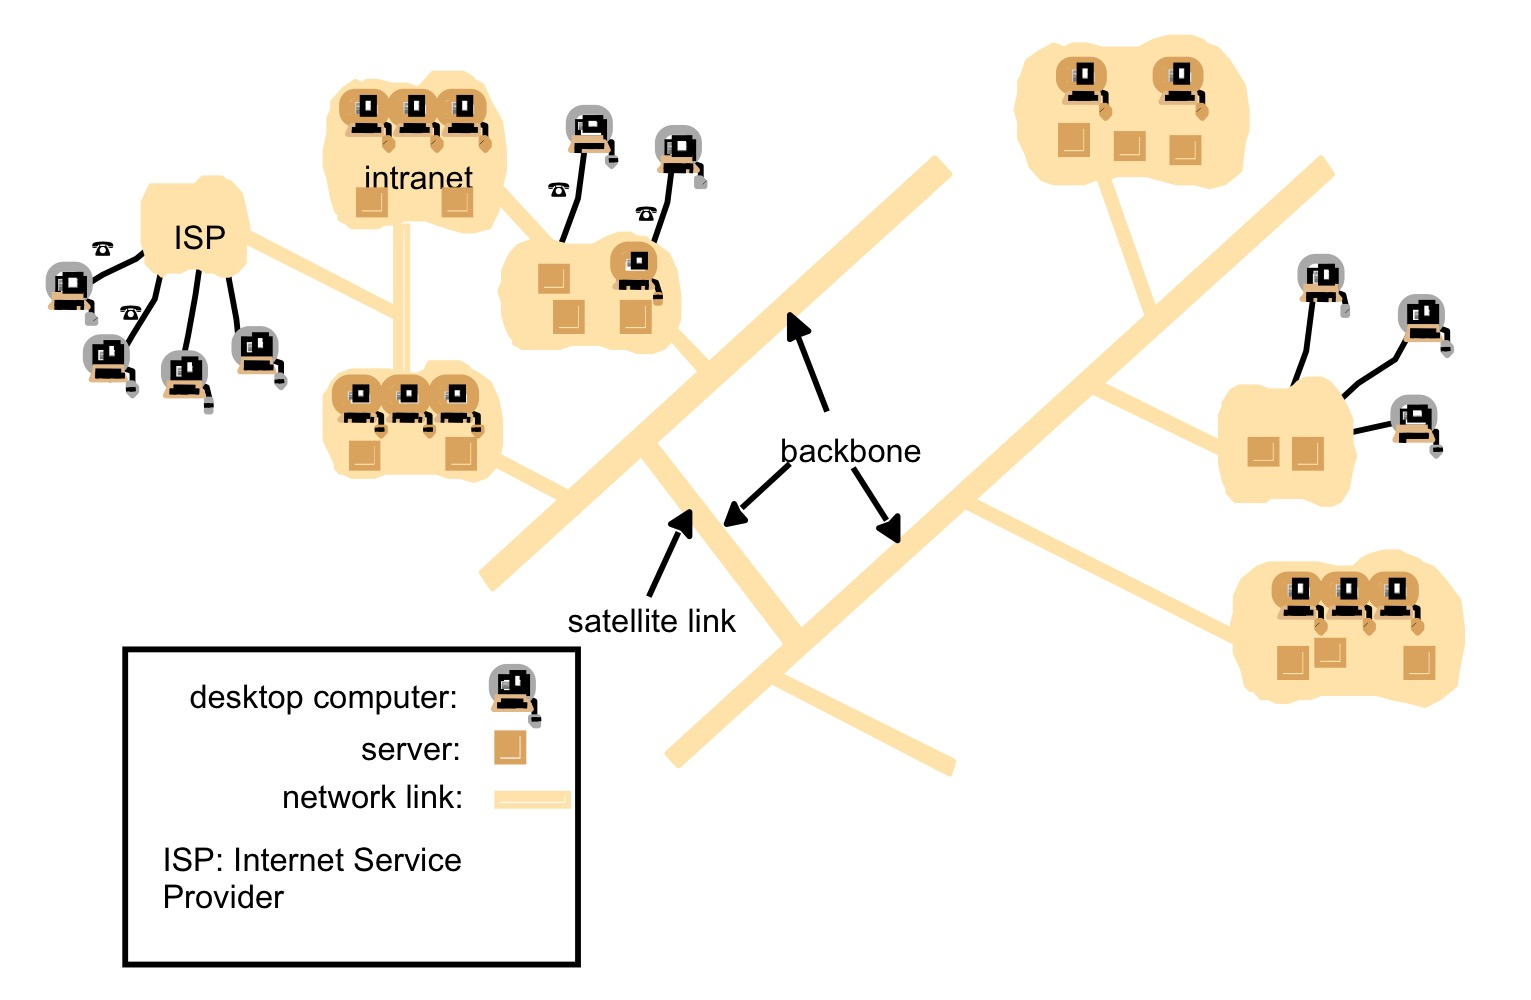
\includegraphics[width=.7\linewidth]{images/introduction/InternetAsDistributedSystem.jpeg}
    \caption{Internet as Distributed System}
\end{figure}

\section{Goals}
\begin{itemize}
    \item \textbf{Economy:} since data can be shared is not necessary to replicate it
    \item \textbf{Software:} the implementation follows particular standards
    \item \textbf{Flexibility:} gives a clear interface to use the system
    \item \textbf{Availability:} the system detects faults and applies recovery operations
    \item \textbf{Performance:} optimal performance in term of:
        \begin{itemize}
            \item Response time
            \item Throughput
            \item Parallelism
            \item Bottleneck reduction
        \end{itemize}
    \item \textbf{Locality and control distribution, security and efficiency} 
    \item \textbf{Transparency}
\end{itemize}

\section{Computer System vs Distributed System}
\begin{itemize}
    \item A \textit{Computer System} is characterised by \textit{single hardware}, system software and application software for data or control
    \item A \textbf{Distributed System} is composed of \textbf{distributed hardware} that can have or not \textbf{distribute software / application} to manage data and control
        \begin{itemize}
            \item \textbf{Distributed hardware:} system composed of \textit{more than two computer systems}, interconnected by a communication network and each \textit{computer is independent} from the others but can \textit{interact with them}
        \end{itemize}
\end{itemize}

\subsection{Control}
Control is essential to manage physical or logical resource on the system, it can be:
\begin{itemize}
    \item \textbf{Centralized:} there is a unique responsible entity
    \item \textbf{Distributed:} computer system on the net cooperate to reach the solution
    \item \textbf{Hierarchical:} system is more scalable since all the functions are subdivided in different modules
\end{itemize}

\section{Open Problems}
\begin{itemize}
    \item \textbf{Data Sharing:} understands how and what resources must be shared and it provides a \textit{system to retrieve them} efficiently
    \item \textbf{Heterogeneity:} enables users to access services and run applications over a heterogeneous collection of computers and networks
    \item \textbf{Concurrency}: several clients could attempt to access a \textit{shared resources} at the same time. The process that administrates shared resources could take one client request at a time.
    \item \textbf{Openness:} \textit{the system is not completely defined}, but it is possible to extend it, for instance \textit{including a new machine}. Open distributed system can be constructed from heterogeneous hardware and software, possibly from different vendors
    \item \textbf{Middleware:} is an intermediate layer that provides an unique public interface
    \item \textbf{Mobility:} it refers to \textit{program code} that can be \textit{transferred} from one computer to another and run at the destination
    \item \textbf{Security:} it is necessary to develop a secure system that \textit{does not allow unauthorized} users to read / write data:
        \begin{itemize}
            \item \textit{Confidentiality:} protection against revelation to unauthorized individuals
            \item \textit{Integrity:} protection against alteration or corruption
            \item \textit{Availability:} protection against interference
        \end{itemize}
    \item \textbf{Scalability:} if it remains stable even if there is a significant increase in the number of resources and users
    \item \textbf{Quality of Services (QoS):} reliability, security and performance of the entire system
    \item \textbf{Fault management:} faults need o be \textit{transparent to the user}. One of the most common recovery algorithm is \textbf{"checkpoint and rollback"} in which we go back the last checkpoint to recover the last consistent state
    \item \textbf{Transparency:} system is perceived as a \textit{set} instead of a \textit{collection of independent components}. Moreover we can analyse different type of transparency:
        \begin{itemize}
            \item \textit{Access:} enables local and remote resources using identical operations
            \item \textit{Location:} enables resources to be accessed without knowledge of their location
            \item \textit{Concurrency:} enables several processes to operate concurrently using shared resources without interface between them
            \item \textit{Replication:} enables multiple instances of resources to be used ti increase reliability and performance without knowledge of the replicas
            \item \textit{Failure:} enable the hiding of faults. Allowing users and application programs to complete their tasks despite the failure of hardware or software components
            \item \textit{Mobility:} allows the movement of resources and clients within a system without affecting the operation of users or programs
            \item \textit{Performance:} allows the system to be reconfigured to improve performance as loads vary
            \item \textit{Scaling:} the system and applications can expand in scale without change to the system structure
        \end{itemize}
\end{itemize}

\section{WWW as Example}
World Wide Web can be seen as a large distributed system based on Internet and its characteristics are:
\begin{itemize}
    \item \textbf{Open System:} it can be \textit{extended and implemented} in new ways without distributing its existing functionality 
    \item \textbf{Client-server architecture}
    \item \textbf{Transparency:}  using DNS it reaches the \textit{location transparency}. With the usage of symbolic server names it is not necessary for the client to know the exact physical address IP of the server
\end{itemize}

\chapter{RDBMS}
The relational data model is based on the concept of storing records of data as rows inside tables.
\begin{itemize}
    \item Each \textbf{row} represents an entity of the real world
    \item And each \textbf{column} is an attribute of interest of these entities
\end{itemize}

\section{Relational Data Model}
\subsection{Database and Relation Schemas}
A relational database consists of a set of tables. Each table has
\begin{itemize}
    \item Predefined name: \textbf{relation symbol}
    \item Set of predefined column names \textbf{the attribute names}
    \begin{itemize}
        \item  Each attribute \(A_i\) ranges over a predefined domain \(dom(A_i)\) such that the values in the column can only come from this domain.
    \end{itemize}
\end{itemize}
A table is then filled row-wise like a tuple with values that represent the state of an entity.

The definition of the attribute names \(A_i\) for the relation symbol \(R\) is called a \textbf{relation schema}; the set of the relation schemas of all relation symbols in the database is then called a \textbf{database schema}.

%relational_database_1 AND relational_database_2
\begin{figure}[!hbp]
    \centering
    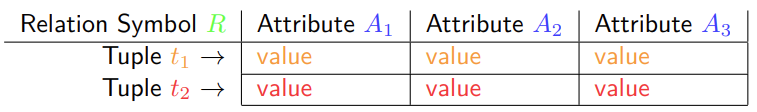
\includegraphics[width=0.90\linewidth]{images/AdvancedDataManagment/rdbms/relational_database_1.png}
    \caption{General example}
\end{figure}
\newpage

\begin{figure}[!hbp]
    \centering
    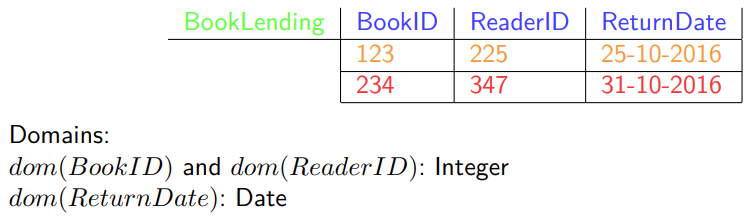
\includegraphics[width=0.90\linewidth]{images/AdvancedDataManagment/rdbms/relational_database_2.png}
    \caption{BookLending example}
\end{figure}

In addition each relation schema can have some type of \textit{constraints} to describe which dependencies between the stored data exist:
\begin{itemize}
    \item \textbf{INTRA relational constraints (local dependencies):} describe dependencies inside a single table, for example be \textit{functional dependencies} – and in particular \textbf{key} constraints
    \item \textbf{INTER relational constraints (global dependencies):} describe dependencies between different tables, for example be \textit{inclusion dependencies} – and in particular \textit{foreign keyindex}
constraints
\end{itemize}

\begin{tcolorbox}
We define a \textbf{Relational Schema} given its
\begin{itemize}
    \item Relation Symbol \(R_i\)
    \item Set of attributes \(A_{i1},...,A_{im}\)
    \item Set of intrarelational/local constraints \(\Sigma_i\)
\end{itemize}
\[R_i = (\{A_{i1},...,A_{im}\}, \Sigma_i)\]
\end{tcolorbox}

\begin{tcolorbox}
We define a \textbf{Database Schema} given its
\begin{itemize}
    \item Database Symbol \(D\)
    \item Set of relation schemas  \(R_1,...,R_m\)
    \item Set of interrelational/global dependencies \(\Sigma\)
\end{itemize}
\[R_i = (\{A_{i1},...,A_{im}\}, \Sigma_i)\]
\end{tcolorbox}

\newpage
\subsubsection{Example Database: Library}
\begin{figure}[!hbp]
    \centering
    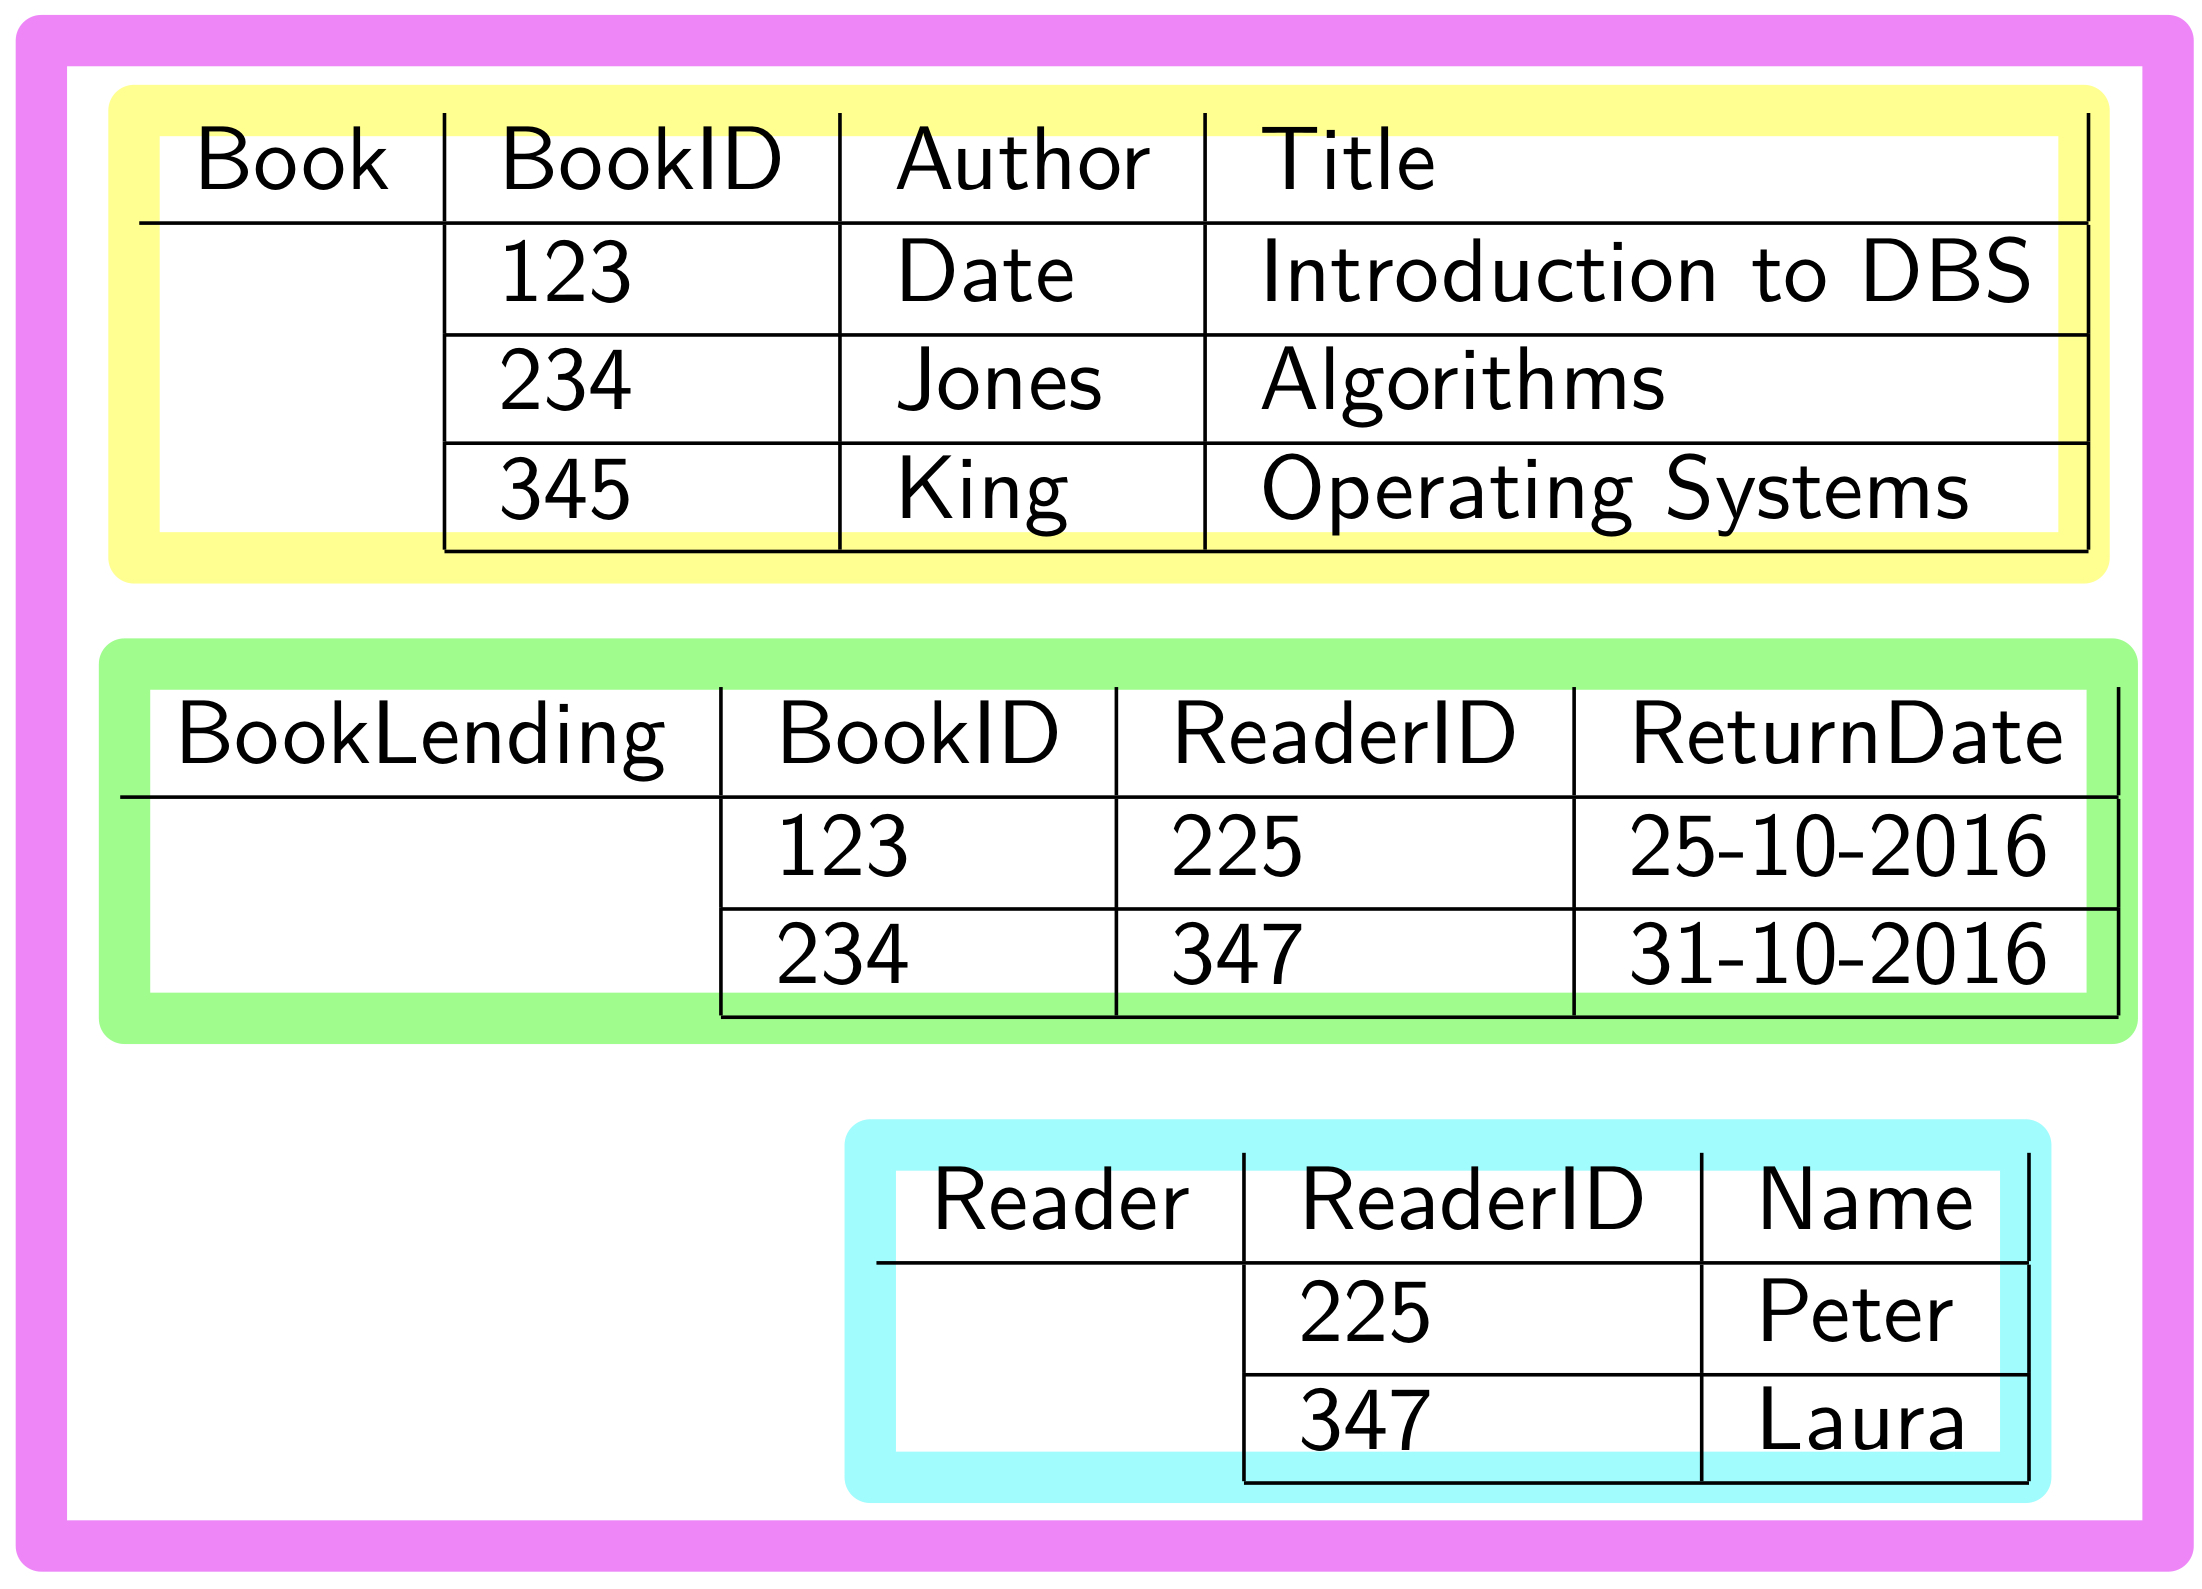
\includegraphics[width=0.60\linewidth]{images/AdvancedDataManagment/rdbms/library_schema_1.jpeg}
    \caption{Library schema example}
\end{figure}

\begin{figure}[!hbp]
    \centering
    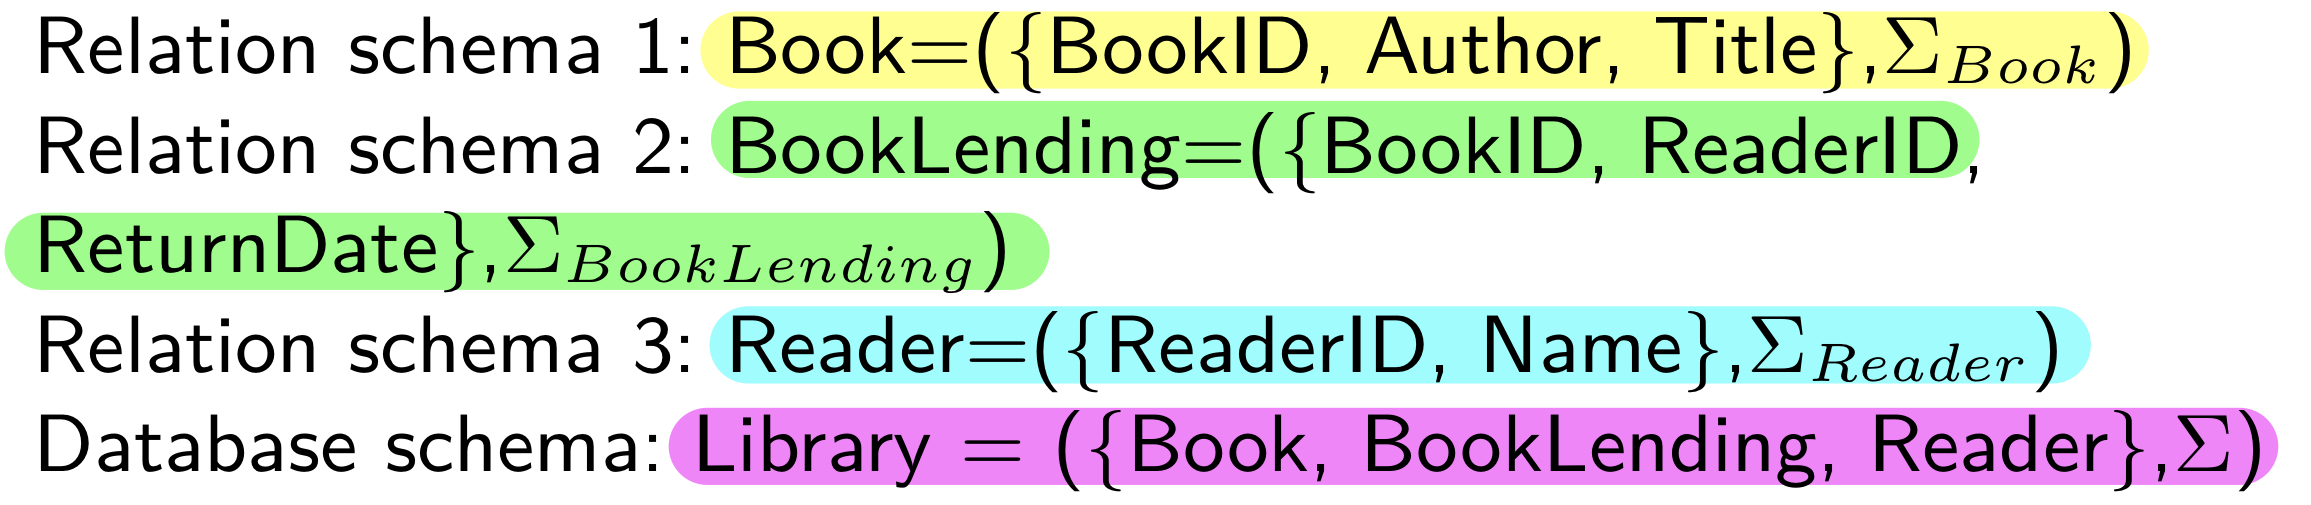
\includegraphics[width=0.70\linewidth]{images/AdvancedDataManagment/rdbms/library_schema2.jpeg}
    \caption{Library schema definition}
\end{figure}

\subsubsection{Example Database: Dependencies}
\begin{figure}[!hbp]
    \centering
    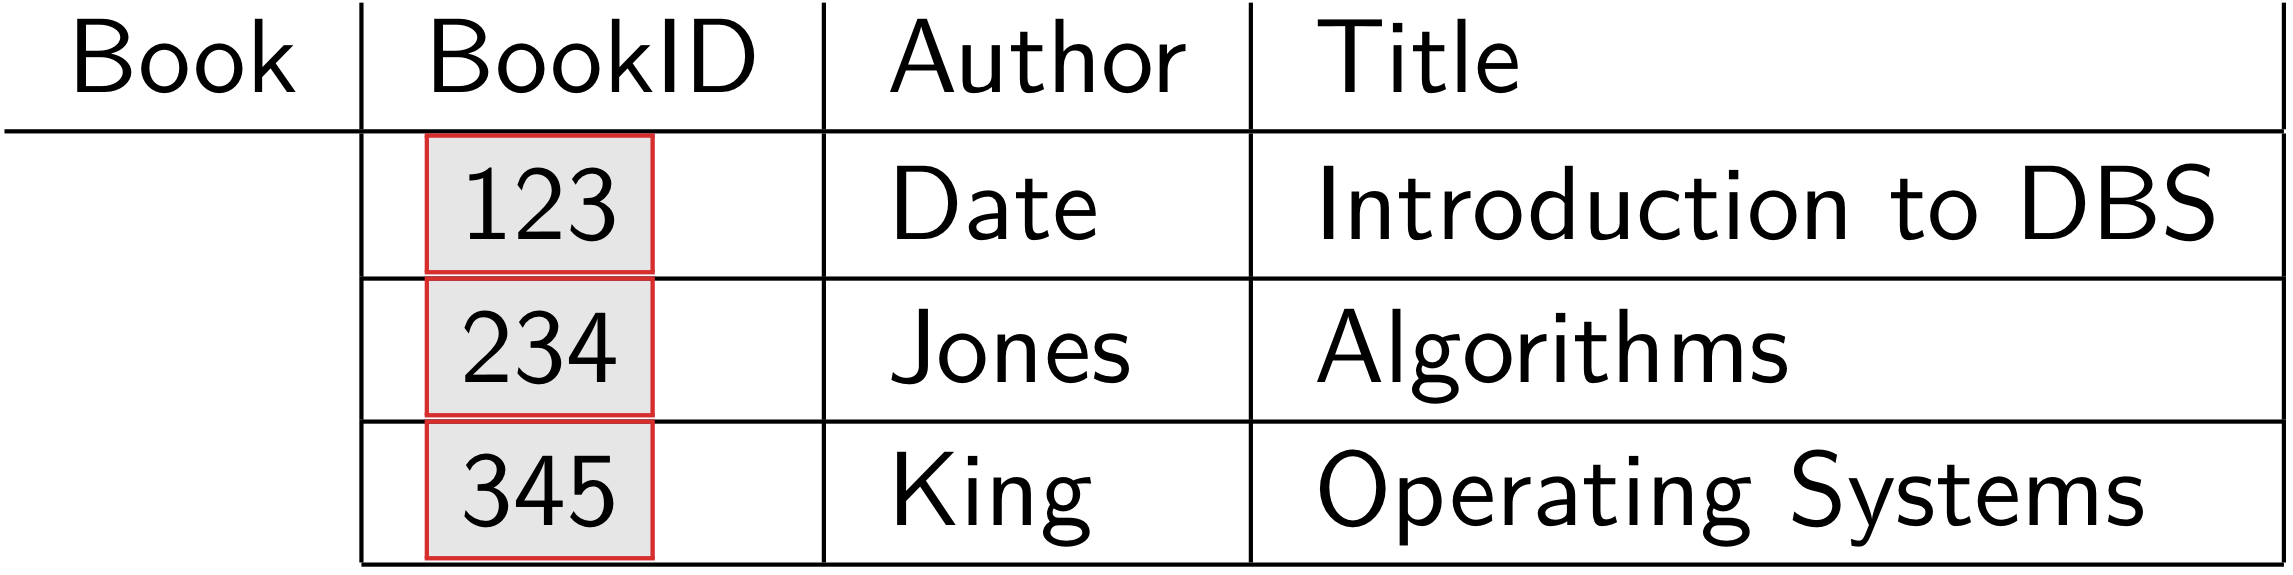
\includegraphics[width=0.50\linewidth]{images/AdvancedDataManagment/rdbms/local_dependencies.jpeg}
    \caption{Book local dependency}
\end{figure}

\begin{figure}[!hbp]
    \centering
    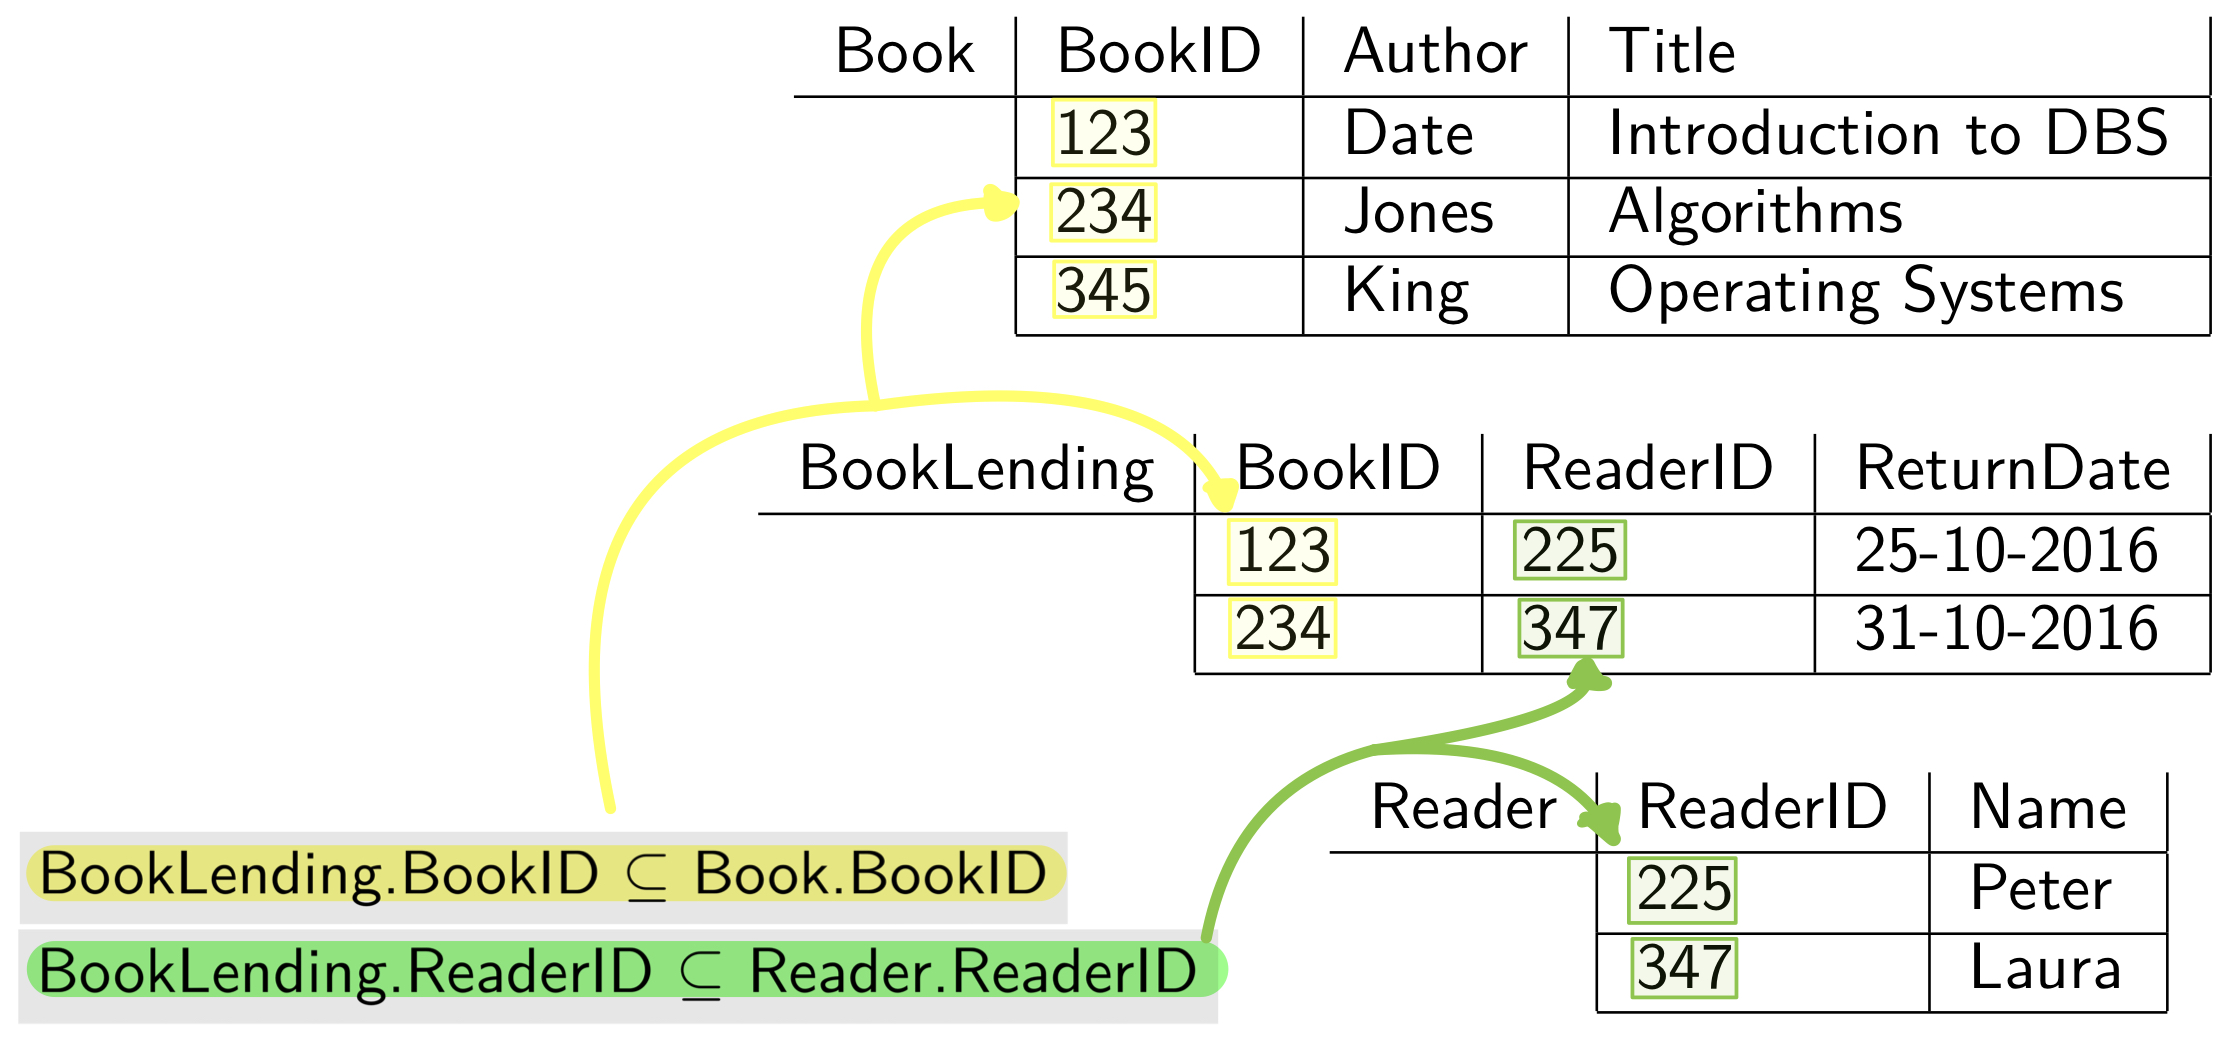
\includegraphics[width=0.70\linewidth]{images/AdvancedDataManagment/rdbms/global_dependencies.jpeg}
    \caption{Library global dependencies}
\end{figure}

\subsection{Mapping ER Models to Schemas}
An ER diagram can be translated into a database schema:
\begin{itemize}
    \item Each \textbf{entity name} corresponds to a relation symbol
    \item Each \textbf{entity attributes} correspond to relation attributes
    \begin{itemize}
        \item Relational data model does not allow multi-valued ad composite attributes
        \item In the case of multi-valued attributes, a new relation schema for each multi-valued attribute created containing additional foreign keys 
    \end{itemize}
    \item \textbf{Composite attributes} should usually be treated as single-valued attributes
    \item \textbf{Relationship} are also translated into a relation schema. In order to be able to map the values from the entities connected by the relationship together, the relation also contains the key attributes of the entities participating in the relationship
\end{itemize}

\subsection{Normalization}
Some database designs are problematic, they contain too many attributes, or tables combine the “wrong” attributes, or tables store data duplicates. These problem cause problem when \textit{inserting}, \textit{deleting} or \textit{updating values}: they are called \textbf{anomalies}, and there are many types like:
\begin{itemize}
    \item \textbf{Insertion anomaly:} we need all attribute values before inserting a tuple
    \item \textbf{Deletion anomaly:} when deleting a tuple, information is lost that we still need in the database
    \item \textbf{Update anomaly:} when data are stored redundantly, values have to be changed in more than one tuple
\end{itemize}
\begin{tcolorbox}
Normalization results in a good distribution of the attributes among the tables and hence normalization helps reduce anomalies. Moreover it depends on the functional dependencies of the relative data table.
\end{tcolorbox}

We have seen 3 main types of Normal form:
\begin{enumerate}
    \item \textbf{First Normal Form (1NF)} that erase the multi-valued and allow composite attributes
    \item \textbf{Second Normal Form (2NF)} in which all non-key attributes are fully dependent on the key attributes
    \item \textbf{Third Normal From (3NF)} in which all non-key attributes are directly dependent on the key attributes
\end{enumerate}

\newpage
\subsubsection{Example of Normalization}
\begin{figure}[!hbp]
    \centering
    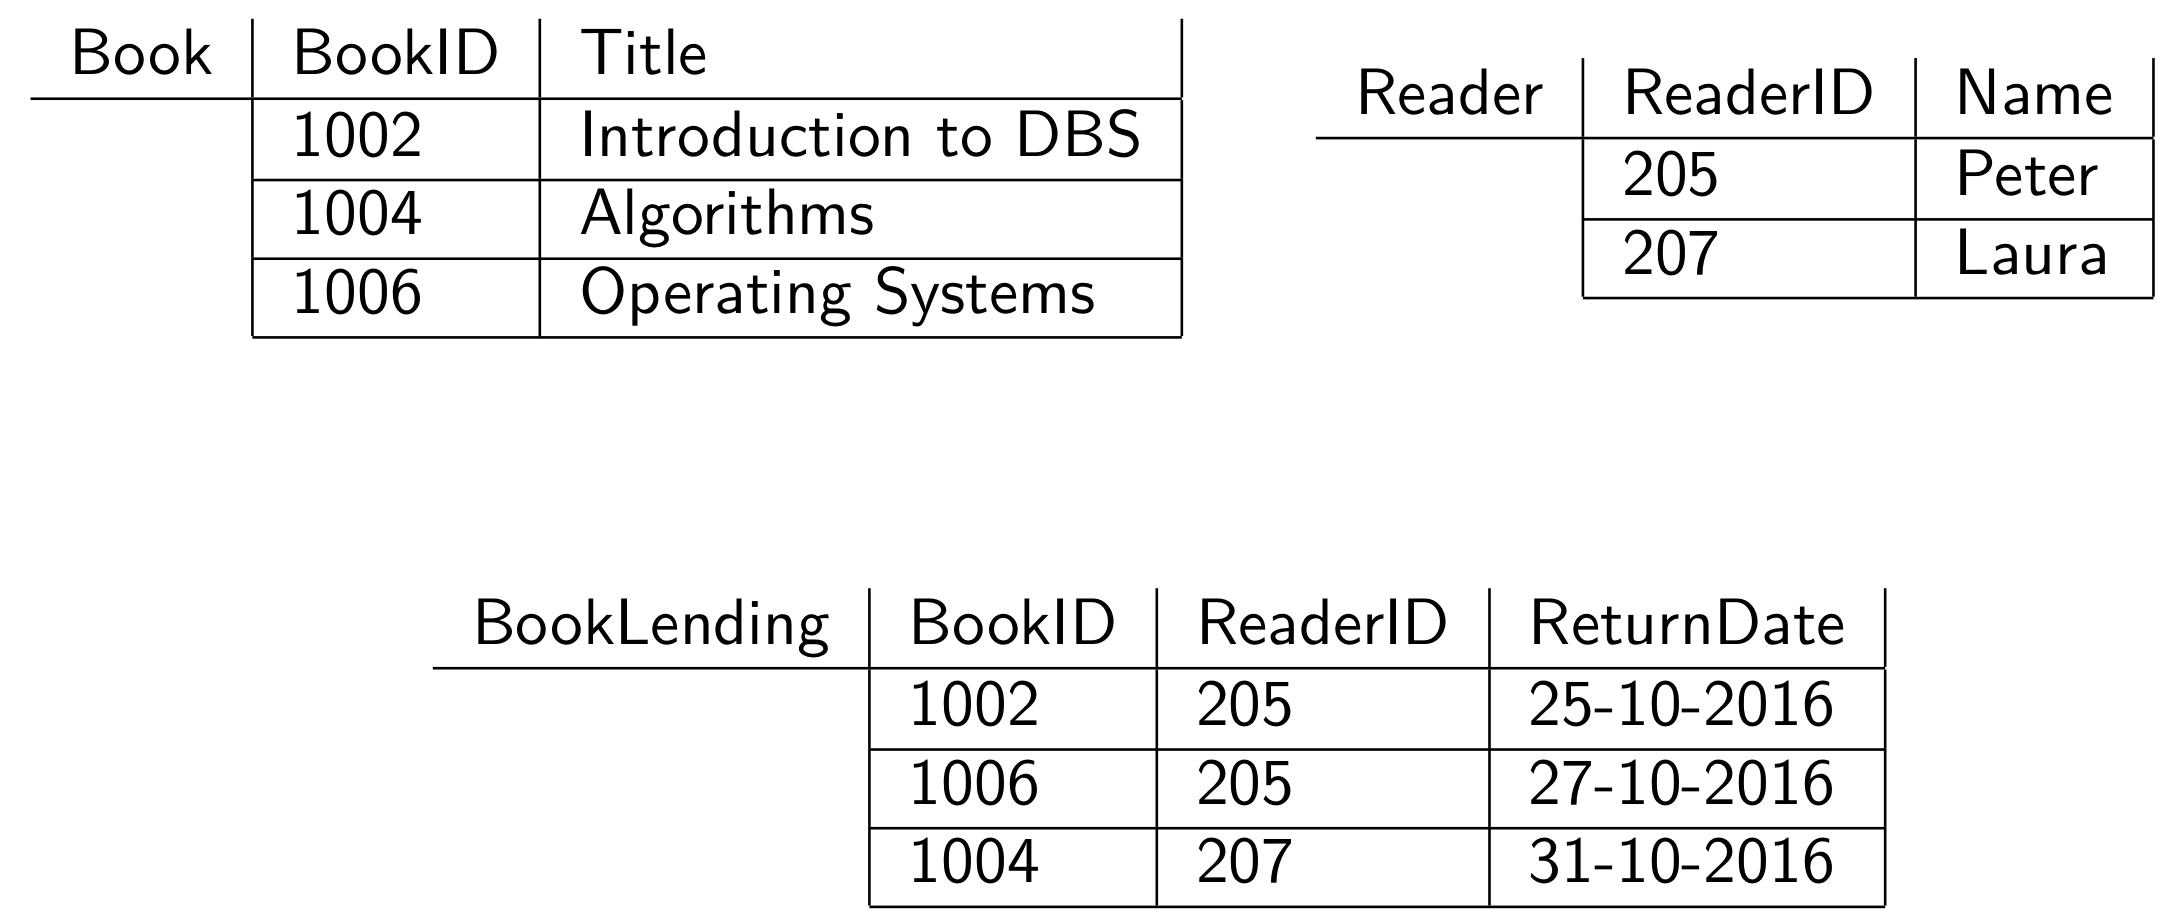
\includegraphics[width=0.70\linewidth]{images/AdvancedDataManagment/rdbms/normalization.jpeg}
    \caption{Library schema normalized}
\end{figure}

\section{Relational Query Languages}
After having design the relational database the next point is to define a strategy to retrieve some information, update and insert additional data in our just born database. We can choose on different strategy, for example taking into account the previous Library example, there is:
\begin{itemize}
    \item \textbf{Natural Language:} "Find all lent books that must be returned before 29-10-2016"
    \item \textbf{Relational Calculus:} Logical formula with variables \(x, y, z:\)
    \[Q(x,y,z) = \{(x,y,z)|\text{BookLending}(x,y,z)\ \land z < \text{29-10-2016}\}\]
    \item \textbf{Relational Algebra} \(\sigma_{ReturnDate<29-10-2016}(BookLending)\)
\end{itemize}

\subsection{Relational Algebra Operators}
\begin{itemize}
    \item \textbf{Projection \(\pi\)} to make some attribute restriction. IDs of readers currently reading a book: \(\pi_{ReaderID}(BookLending)\)
    \item \textbf{Selection \(\sigma\)} with condition on answer tuples. All books to be returned before 29-10-2016: \(\sigma_{ReturnDate<29-10-2016}(BookLending)\)
    \item \textbf{Renaming \(\rho\)} to assign a new attribute name. Rename ReturnDate to DueDate \(\rho_{DueDate\leftarrow ReturnDate}(BookLending)\)
    \item \textbf{Union, Difference and Intersection}
    \item \textbf{Natural Join \(\Join\)} to combine two tables on attributes with same name. All information on Books currently lent: \(\text{Book} \Join \text{BookLending}\)
\end{itemize}
One more thing to note about relational algebra is that an algebra query can be illustrated by a tree:
\begin{itemize}
    \item \textit{Inner nodes} are the algebra operators
    \item \textit{Leaf nodes} are the relation symbol
\end{itemize}

\section{Transaction}
A transaction can be characterized as a sequence of read and write operations on a database; this sequence of operations must be treated as a whole and cannot be interrupted. A transaction moves our system state from one into an other. The following propriety are ensured:
\begin{itemize}
    \item \textbf{Logical data integrity:} are the written values correct and final results of a computation?
    \item \textbf{Physical data integrity \& Recovery:} how can correct values be restored after a system crash?
    \item \textbf{Multi-user support:} how can users concurrently operate on the same database without interfering?
\end{itemize}
To achieve physical data integrity and as part of the recovery management, the database system maintains a \textbf{transaction log}. It stores which operation of which transaction is currently being executed. After a system restart all operations of uncommitted transactions have to be undone. The transaction log also has to take care of committed transactions: If all results of a transaction have been computed but disk writing is interrupted, after a system restart all affected computations of the transaction have to be redone and then stored to disk.


Most RDBMS manage transactions according to the following properties:
\begin{itemize}
    \item \textbf{A}tomicity: either execute all operations or none of them
    \item \textbf{C}onsistency: after the transaction, all values in the database are correct
    \item \textbf{I}solation: concurrent transactions of different users do not interfere
    \item \textbf{D}urability: all transaction results persist in the database even after a system crash
\end{itemize}


\chapter{New Requirements, NOSQL}
\section{Weaknesses of the RDM}
The following weaknesses can become an issue when using the relational data model
\begin{itemize}
    \item \textbf{Inadequate Representation of Data:} 
    \begin{itemize}
        \item Translating arbitrary data into the \textit{relational table} format is not an easy task, since there are complex formats like XML and unstructured text documents, so squeezing data into row and columns need some additional attention
        \item The efficiency of retrieval is associated also to the data representation since it might have to be recombined from several tables
        \item Due to normalization data belonging to a single entity might end up in several different tables
    \end{itemize}
    \item \textbf{Semantic Overloading:} entities as well as relationships between entities are both mapped to relations in a database schema. In our final database schema, both the entities and the relationships were contained as relation schemas.
    \item \textbf{Weak Support for Recursion:} in the relational data model it is diffcult to execute recursive queries that need to join. The purpose of a recursive query is to compute the \textit{transitive closure} of some table attributes. Costly to compute in a real RDBMS.
    \item \textbf{Homogeneous data structure:} the relational data model requires both \textit{horizontal} and \textit{vertical} homogeneity:
    \begin{itemize}
        \item \textit{Horizontal homogeneity:} all tuples have to range over the same set of attributes
        \item \textit{Vertical homogeneity:} values in one column have to come from the same predefined attribute domain
    \end{itemize}
    Mixing values from different domains in one column is not allowed
\end{itemize}

\section{Weaknesses of RDBMSs}
\begin{itemize}
    \item \textbf{Infrequent updates:} RDBMSs are designed for frequent queries but very infrequent updates 
    \item \textbf{SQL dialects:} not all RDBMSs fully support the standard and some deliberately use their own syntax
    \item \textbf{Restricted data types:} RDBMS can be considered quite inflexible regarding the support of modern data types or formats
    \item \textbf{Declarative access:} SQL is that queries are usually \textit{declaratively} expressed based on the (expected) content in the database tables. However, other data formats might require a non-declarative access
    \item \textbf{Short-lived transactions:} the typical RDBMS transaction is however very short-lived. The implemented transaction management mechanisms are usually not suited for long-term transactions. However, the support for long-term transactions is in particular important for data stream processing where queries are periodically executed on continuous streams of data
    \item \textbf{Lower throughput:} handling massive amounts of data, achieving a suffciently high data throughput might not be possible as good as one would require with an RDBMS
    \item \textbf{Rigid schema:} schema evolution is poorly supported: Changes in the relation schemas are diffcult and costly
    \item \textbf{Non-versioned data:} versioning of data is disregarded by conventional RDBMSs
\end{itemize}

\section{New Data Management Challenges}
Some of the new challenges for database management are the
following:
\begin{itemize}
    \item \textbf{Complexity:} data are organized in complex structures like social network and thus graph structure
    \item \textbf{Schema independence:} documents can be processed without a given schema definition, so data can be structured in an arbitrary way without complying with any prescribed format
    \item \textbf{Sparseness:} if there is an (optional) schema for a data set, it may happen that a lot of data items are not available
    \item \textbf{Self-descriptiveness:} As a consequence on schema independence and sparseness, metadata are attached to individual values in order to enable data processing
    \item \textbf{Variability:} data are \textit{constantly changing}, DBMS has to handle frequent data modifications in the form of insertions, updates and deletions
    \item \textbf{Scalability:} data are distributed on a huge number of interconnected servers. Moreover, the database system has to support flexible horizontal scaling : servers can leave the network and new servers can enter the network on demand.
    \item \textbf{Volume:} large data volumes have to be processed
\end{itemize}

\section{NOSQL}
Non-relational databases have been developed as a reaction to these challenges and new requirements. Historically the term “NoSQL” applied to database systems that offered query languages and access methods other than the standard SQL. NOSQL covers database systems that:
\begin{itemize}
    \item Have data models other than the conventional relational tables
    \item Support programmatic access to the database system or query languages other than SQL
    \item Can cope with schema evolution
    \item Support data distribution
    \item Do not strictly adhere to the ACID properties
\end{itemize}

\chapter{Key-value Stores}
Key-value stores are specialized for the efficient storage of simple key value pairs. Parallel processing of key-value pairs has been popularized with the \textbf{Map-Reduce paradigm}.

\section{Key-Value Storage}
A key-value pair is a tuple of two strings $\langle key, value \rangle$. 
\begin{itemize}
    \item The key is the identifier and has to be unique.
    \item You can retrieve a value from the store by simply specifying the key; and you can delete a key-value pair by specifying the key.
    \item  A key-value store is the prototype of a \textbf{schemaless} database system: you can put arbitrary key-value pairs into the store and no restrictions are enforced on the format or structure of the value.
\end{itemize} 

Key-value store basically only offers three operations:
\begin{itemize}
    \item \textit{reading:} value = store.get(key)
    \item \textit{writing:} store.put(key, value)
    \item \textit{deleting:} store.delete(key)
\end{itemize}
It is \textbf{“simple but quick”}, indeed data are stored in a simple key-value structure and the key-value store is ignorant of the content of the value part. Here some characteristics:
\begin{itemize}
    \item Simple format is that data can easily be distributed among several database servers
    \item Key-value stores are good for “data-intensive” applications, like session management or shopping carts
    \item Most key-value stores, values are allowed to have other data types than just strings
    \item Some key-value stores also support data formats like XML or JSON
\end{itemize}

\subsection{Map-Reduce}
\begin{itemize}
    \item \textbf{Map:} transform a given list into an other with all the elements passed to a given function
    \item \textbf{Reduce:} given a list and a function they produce a single value using all list elements
\end{itemize}
The basic elements of map-reduce are four functions that operate on key-value pairs split, map, shuffle and reduce.
While \textit{split} and \textit{shuffle} are more or less generic functions that can have the same implementation for all applications, the other two – \textit{map} and \textit{reduce} – are \textbf{highly application-dependent} and have to be implemented by the user of the map-reduce framework.

Map and reduce are executed by \textit{several worker processes} running on several servers; one of the workers is the \textbf{master} who \textit{assigns} new map or reduce tasks to idle workers.
\begin{itemize}
    \item \textbf{Split} input key-value pairs into disjunct subsets and assign each subset to a worker process 
    \item Let workers compute the \textbf{map} function on each of its input splits that outputs intermediate key-value pairs
    \item The \textbf{shuffle} groups all intermediate values by key and assign each group to a worker
    \item Finally \textbf{reduce} values of each group and return the result
\end{itemize}

\subsubsection{Example, counting occurrences of words in a document}
\begin{figure}[!hbp]
    \centering
    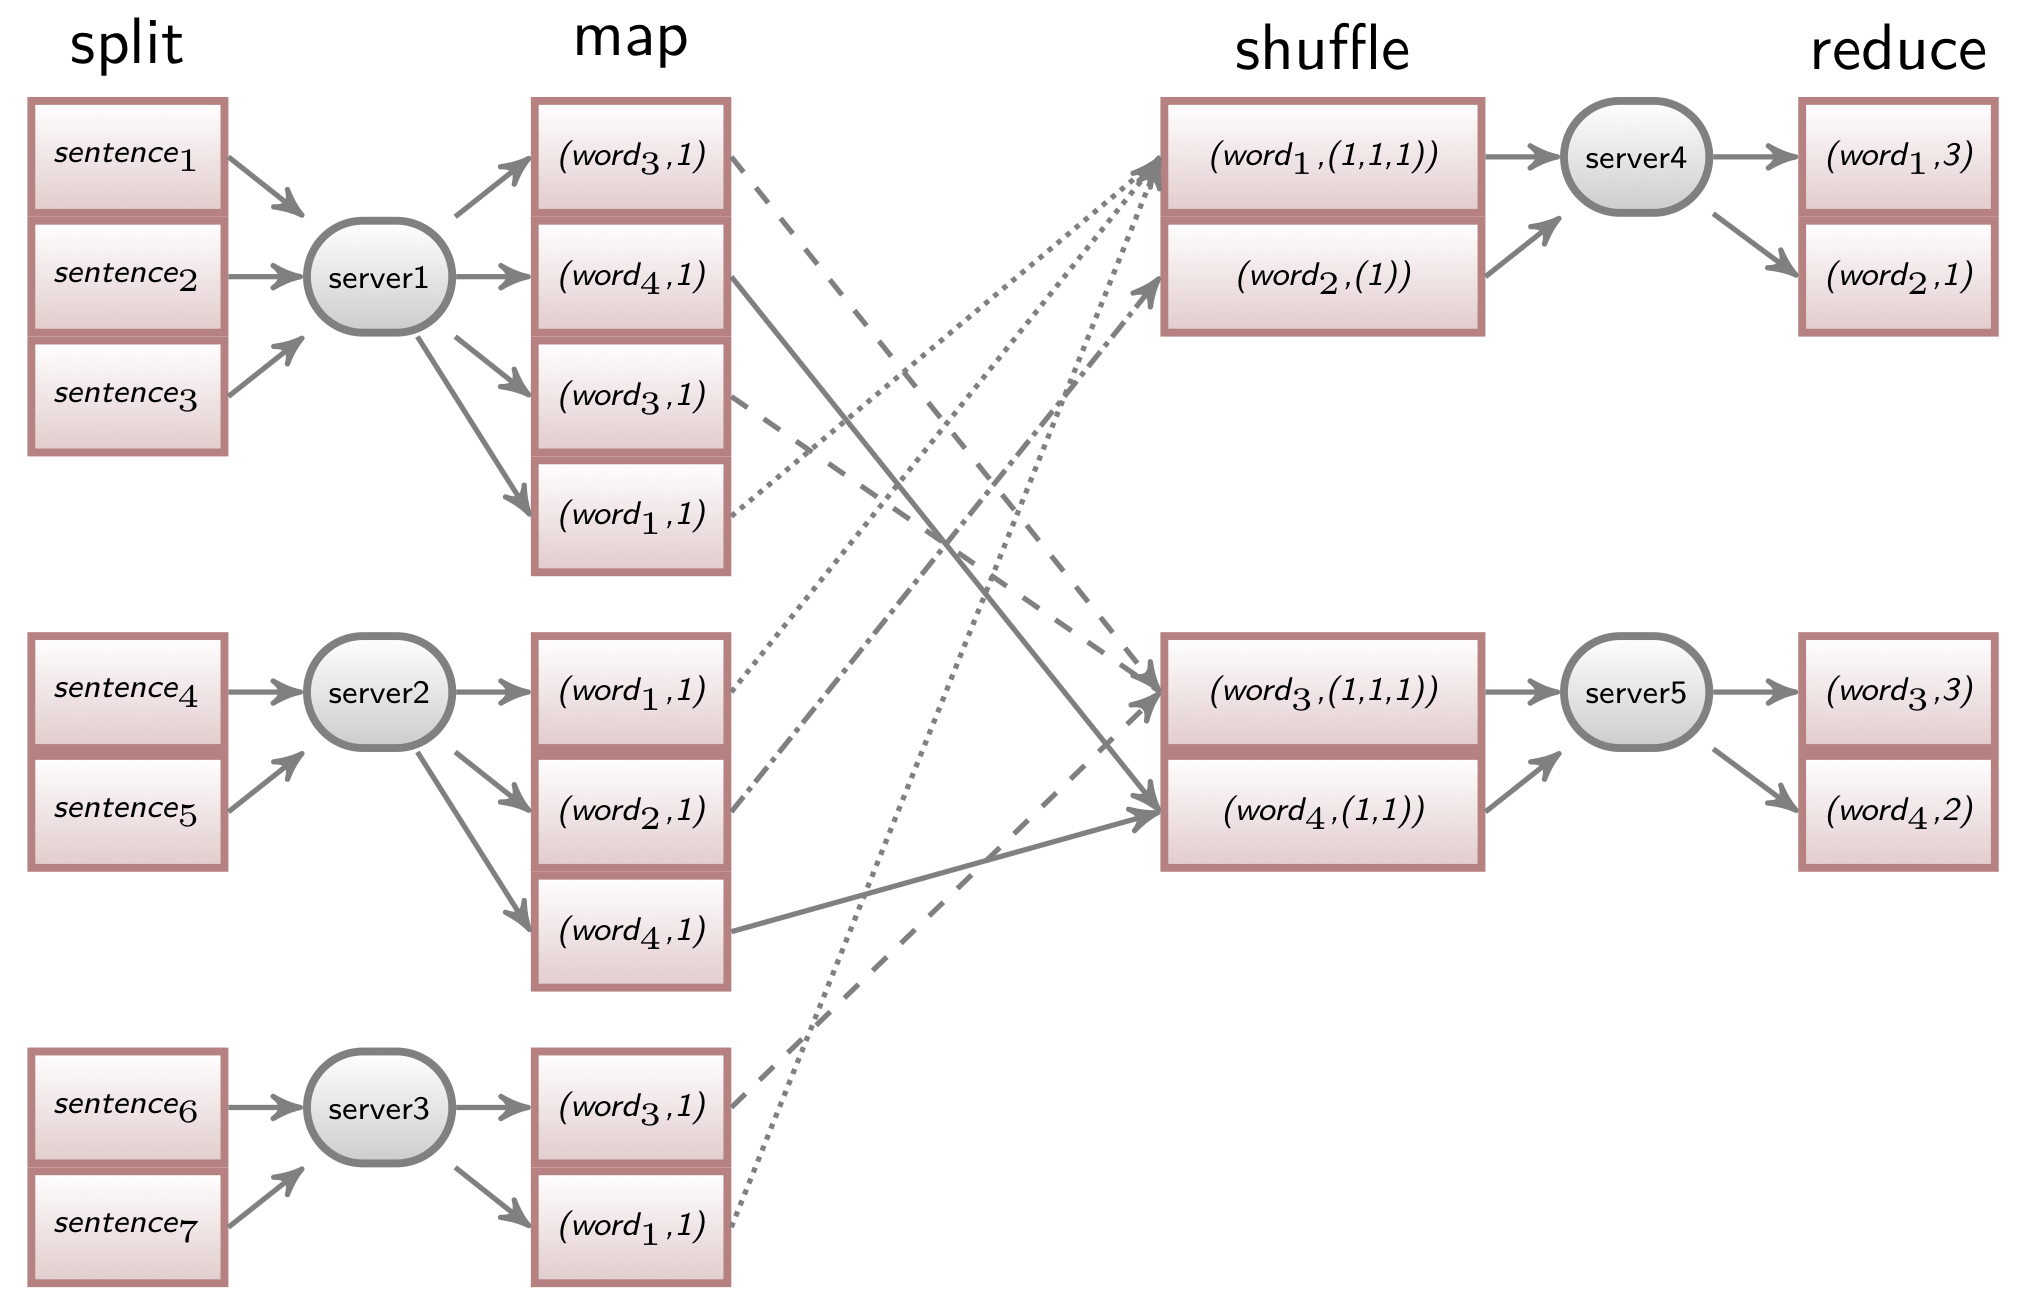
\includegraphics[width=0.70\linewidth]{images/AdvancedDataManagment/key_value_store/map_reduce.jpeg}
    \caption{Example of Map Reduce}
\end{figure}

\newpage
\begin{enumerate}
    \item \textbf{Split function} splits the document into sentences; each sentence is assigned to a worker process
    \item Worker thread starts a \textbf{map function} for each sentence. 
    \begin{itemize}
        \item It \textit{parses} a sentence and for \textit{each word} \(word_i\), the worker thread emits a \textit{key-value pair} \((word_i, 1)\) to indicate it encountered \(word_i\) once
        \item Intermediate result stored locally
    \end{itemize}
    \item In the \textbf{suffle phase} local intermediate results are read and grouped by words
    \begin{itemize}
        \item The 1-values for each word are concatenated into a list
        \item Key-value pair where the word \(word_i\) is the \textbf{key} and the \textbf{value} is a \textit{list of 1s} corresponding to individual occurrences of the word in all sentences
        \item Each word is assigned to a worker process
    \end{itemize}
    \item The \textbf{reduce function} calculates the total number of occurrences by \textit{summing the 1s}. The final results will look like a sequence of key-value pair \((word_i, sum_i)\)
\end{enumerate}

More formally:
\begin{itemize}
    \item \textbf{Split:} \textit{list ! list\((key_1, value_1)\)}:  split maps some input text to a list of key-value pairs
    \item \textbf{Map:} \((key_1, value_1)\) ! \(list(key_2, value_2)\): map processes one key-value pair and maps it to a list of key-value pairs
    \item \textbf{Shuffle:} \(list(key_2, value_2)\) ! (\(key_2\), \(list(value_2)\)): shuffle groups the individual key-value pairs by key and appends to each key a list that is a concatenation of the values of the individual pairs
    \item \textbf{Reduce:} (\(key_2, list(value_2)\)) ! (\(key_3, value_3\)): reduce aggregates a list of values into a single one
\end{itemize}

\subsubsection{Possible optimizations}
\begin{itemize}
    \item \textbf{Parallelization:} the map and as well as the reduce task can be run in parallel by different concurrent worker processes and even on multiple servers
    \item \textbf{Partitioning:} usually there are more reduce tasks to be executed than workers available. That is, each worker has to execute several reduce task on a set of different keys
    
    \newpage
    
    \item \textbf{Combination:} instead of locally storing lots of intermediate results of the map processes which later on have to be shuffled to other workers over the network. \textit{Combine} task can be run locally on each worker after the map phase, it  is similar to the reduce function as it groups the intermediate results by key and combines their values
    
    \begin{figure}[!hbp]
        \centering
        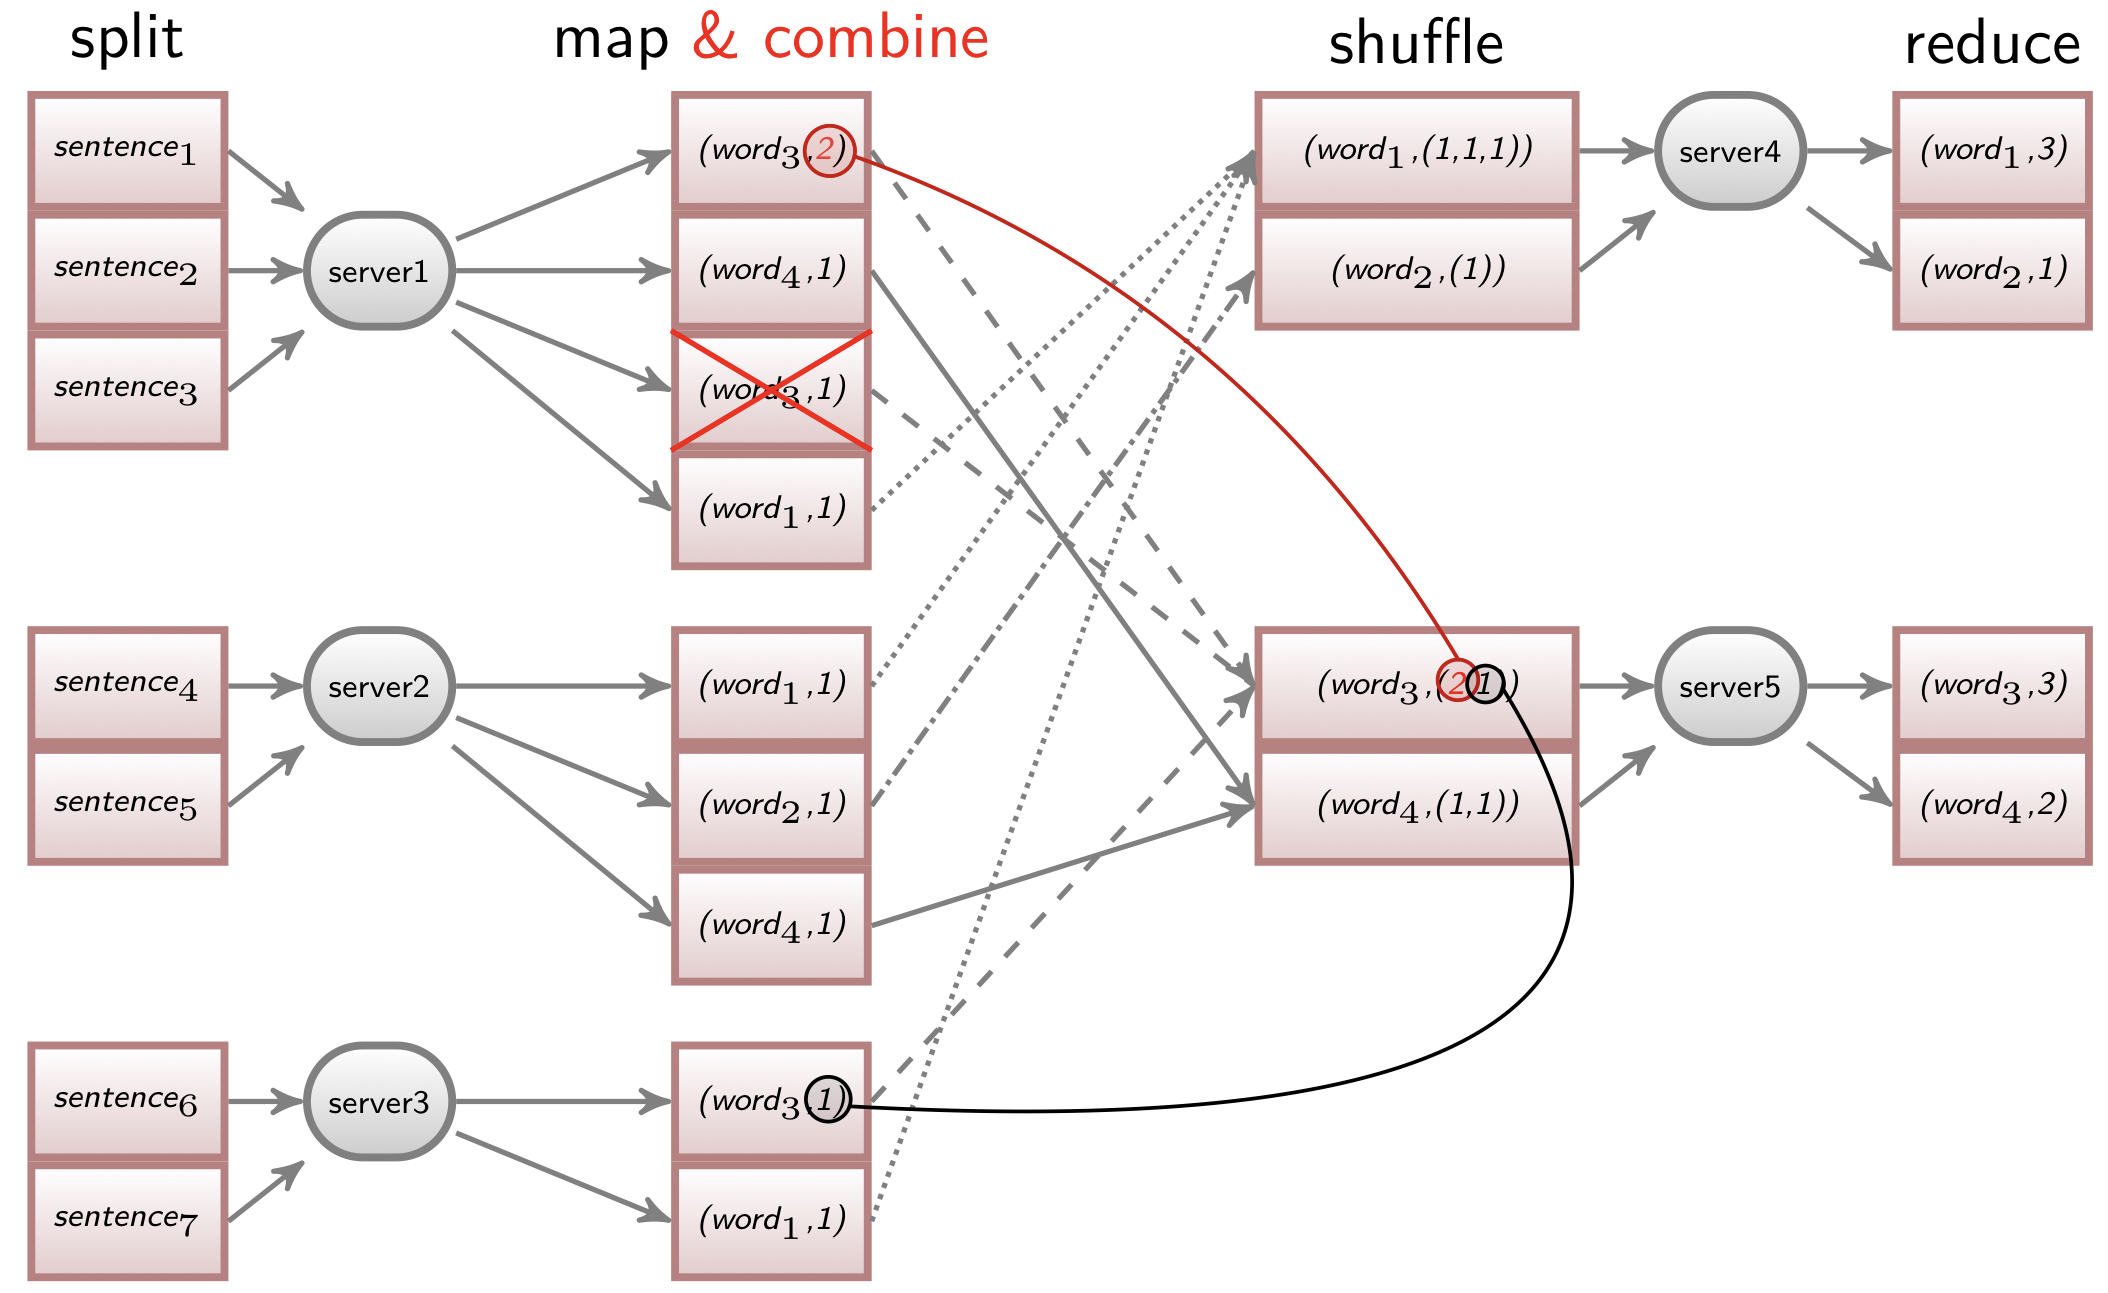
\includegraphics[width=0.70\linewidth]{images/AdvancedDataManagment/key_value_store/combination.jpeg}
        \caption{Example of Combination Map Reduce}
    \end{figure}
    
    \item \textbf{Data Locality:} transmitting data to a worker over the network is costly, thus the \textit{master} can take the location of data into account before assigning a task to a worker
    \item \textbf{Incremental Map-Reduce:} input data might be generated dynamically over a longer period of time. To improve evaluation of such data, the four steps can be interleaved and final results be obtained incrementally
\end{itemize}

\chapter{Column Stores}
\textbf{Row Store:}
\begin{itemize}
    \item Data are stored in tables and on disk
    \item Stored consecutively
    \item Used in most RDBMs
\end{itemize}
\textbf{Column Store:}
\begin{itemize}
    \item Column oriented relational database
    \item Data are stored in tables but on disk
    \item Stored consecutively
\end{itemize}
Column store work very well for certain queries type like queries that can be executed on compressed data, indeed columns stores have the advantage of both a \textit{compact storage} as well as \textit{efficient query execution}.

\section{Column-Wise Storage}
We take up our tiny library example to illustrate the differences:
\begin{figure}[!hbp]
    \centering
    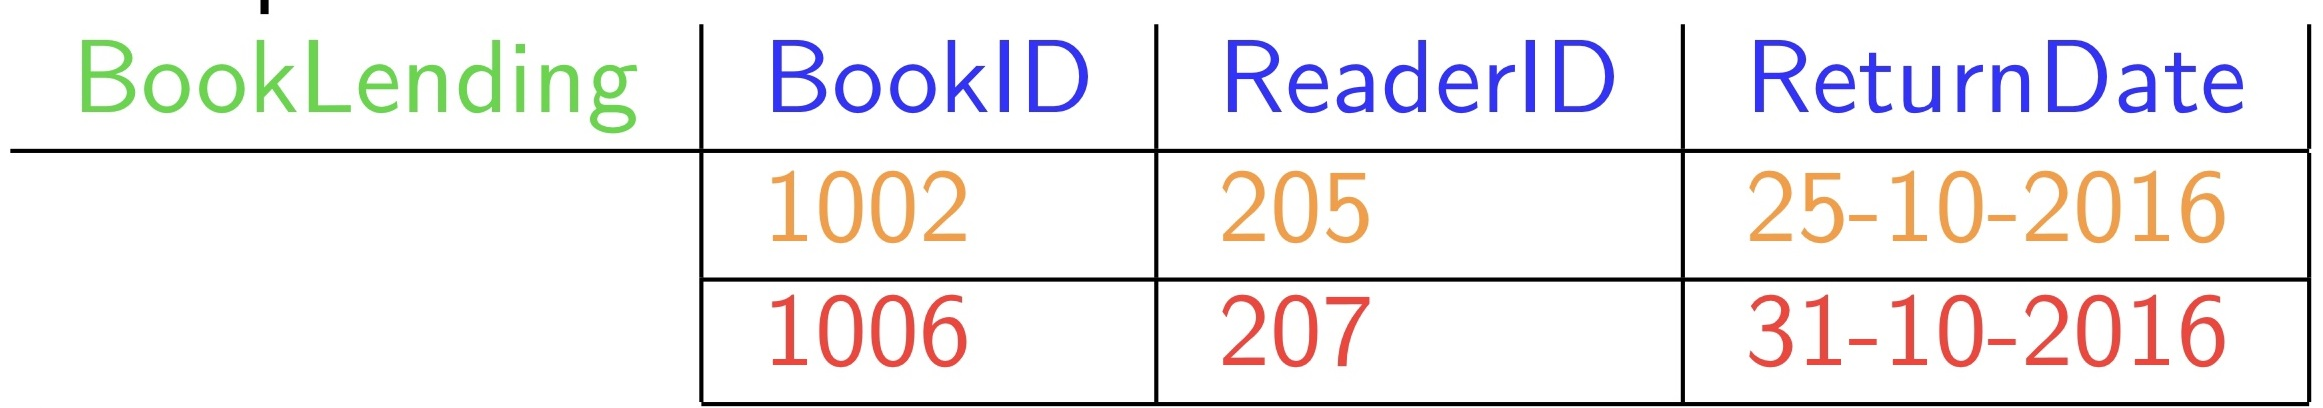
\includegraphics[width=0.60\linewidth]{images/AdvancedDataManagment/column_stores/library_example.jpeg}
    \caption{BookLending example}
\end{figure}

Storage order in row store:

\centerline{\textcolor{orange}{1002, 205, 25-10-2016}, \textcolor{red}{1006, 207, 31-10-2016}}

Storage order in column store:

\centerline{
\textcolor{orange}{1002}, \textcolor{red}{1006},
\textcolor{orange}{205}, \textcolor{red}{207},
\textcolor{orange}{25-10-2016}, \textcolor{red}{31-10-2016}
}
\textbf{Advantages} of column stores are for example:
\begin{itemize}
    \item \textbf{Buffer management:} only columns (attributes) that are needed are read from disk into main memory, because a single memory page ideally contains all values of a column.
    \begin{itemize}
        \item In row stores memory page might contain also other attributes, so data is fetched unnecessarily
    \end{itemize}
    \item \textbf{Homogeneity:} values in a column have the same type. This is why they can be compressed better when stored consecutively.
    \begin{itemize}
        \item In row stores values from different attribute domains are mixed in a row, so compression is not as good
    \end{itemize}
    \item \textbf{Data locality:} iterating or aggregating over values in a column can be done quickly.
    \begin{itemize}
        \item In row stores values have to be read and picked out from different tuples
    \end{itemize}
    \item \textbf{Column insertion:} adding new columns to a table is easy because they just can be appended to the existing ones
    \begin{itemize}
        \item  In row store, storage reorganization it necessary to append a new column value to each tuple
    \end{itemize}
\end{itemize}

\textbf{Disadvantages} of column stores are:
\begin{itemize}
    \item \textbf{Tuple reconstruction:} combining values from several columns is costly because “tuple reconstruction” has to be performed
    \begin{itemize}
        \item In row store, tuple reconstruction is not necessary because values of a tuple are stored consecutively
    \end{itemize}
    \item \textbf{Tuple insertion:} inserting a new tuple is costly
    \begin{itemize}
        \item In row store, the new tuple is appended to the existing ones and the new values are stored consecutively
    \end{itemize}
\end{itemize}

\subsection{Column Compression}
\begin{itemize}
    \item Values in a column range over the same attribute domain; that is, the have the same data type.
    \item Columns may contain lots of repetitions of individual values or sequences of values.
    \item These are two reasons why compression can be more effective on columns.
    \item Storage space needed in a column store may be less than storage space needed in a row store with the same data.
\end{itemize}
\newpage
 Having said that we can introduce five option for column data compression: 
\begin{itemize}
    \item \textbf{Run-length encoding:}
    \begin{itemize}
        \item The run-length of a value denotes how many repetitions of the value are stored consecutively
        \item We will store the value together with its starting row and its run-length
        \item This encoding is most efficient for long runs of repetitive values
    \end{itemize}
    \begin{figure}[!hbp]
        \centering
        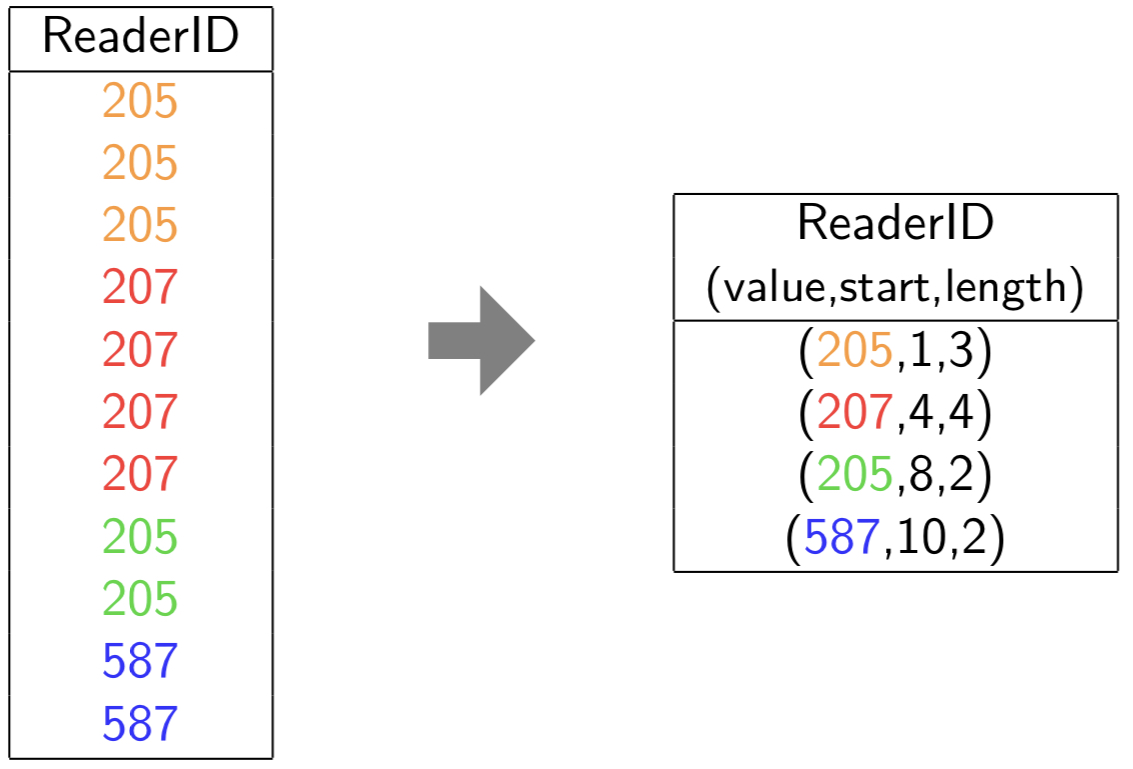
\includegraphics[width=0.60\linewidth]{images/AdvancedDataManagment/column_stores/run-length_encoding.jpeg}
        \caption{Run-length encoding example}
    \end{figure}
        
    
    \item \textbf{Bit-vector encoding:} 
    \begin{itemize}
        \item For each value in the column we create a bit vector with one bit for each row
        \item In each vector cell if the value is 1, it means the presence of the value in the column
        \item This encoding is most efficient for relatively few distinct values and hence relatively few bit vectors
    \end{itemize}
    
    
    \begin{figure}[!hbp]
        \centering
        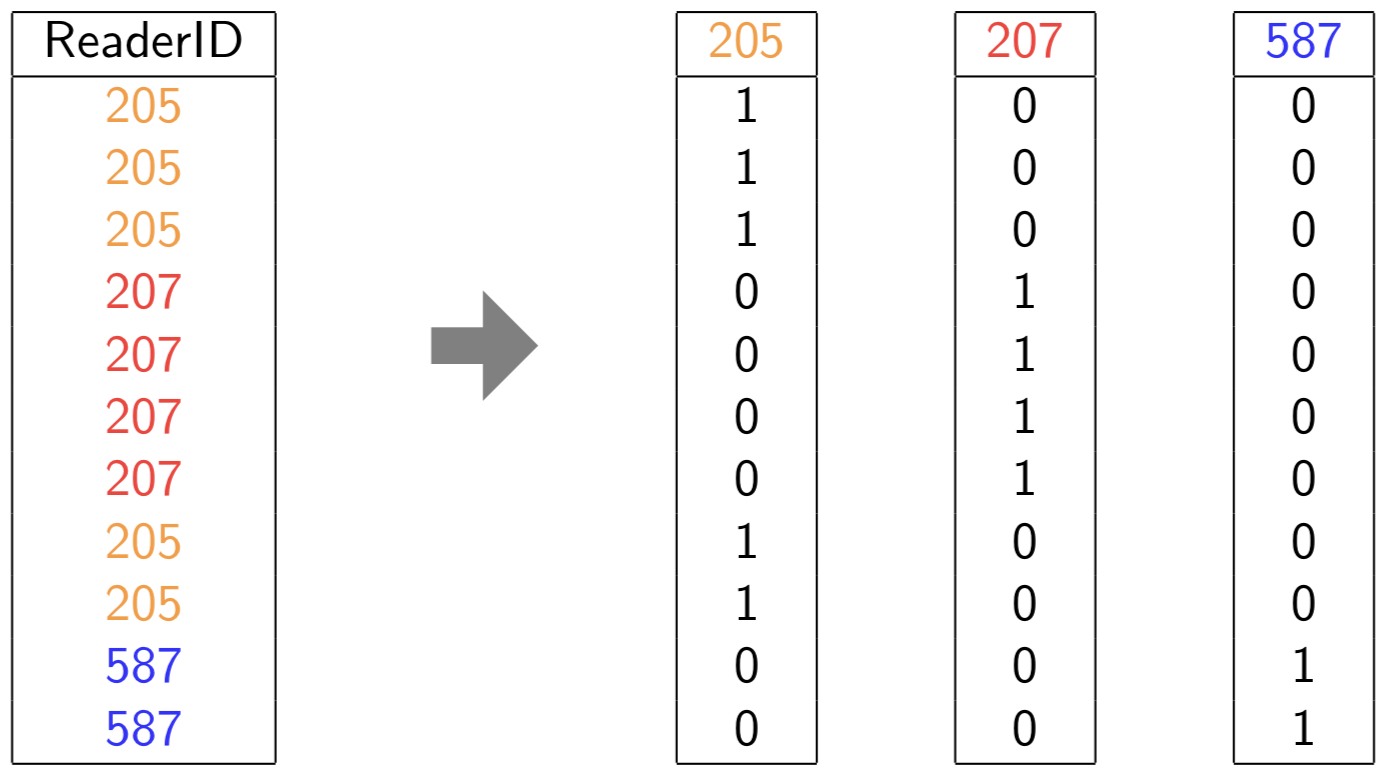
\includegraphics[width=0.60\linewidth]{images/AdvancedDataManagment/column_stores/bit_vector_encoding.jpeg}
        \caption{Bit vector encoding example}
    \end{figure}
    
    \newpage
    \item \textbf{Dictionary encoding:} 
    \begin{itemize}
        \item We replace long values by shorter placeholders and maintain a dictionary to map the placeholders back to the original values
        \begin{figure}[!hbp]
            \centering
            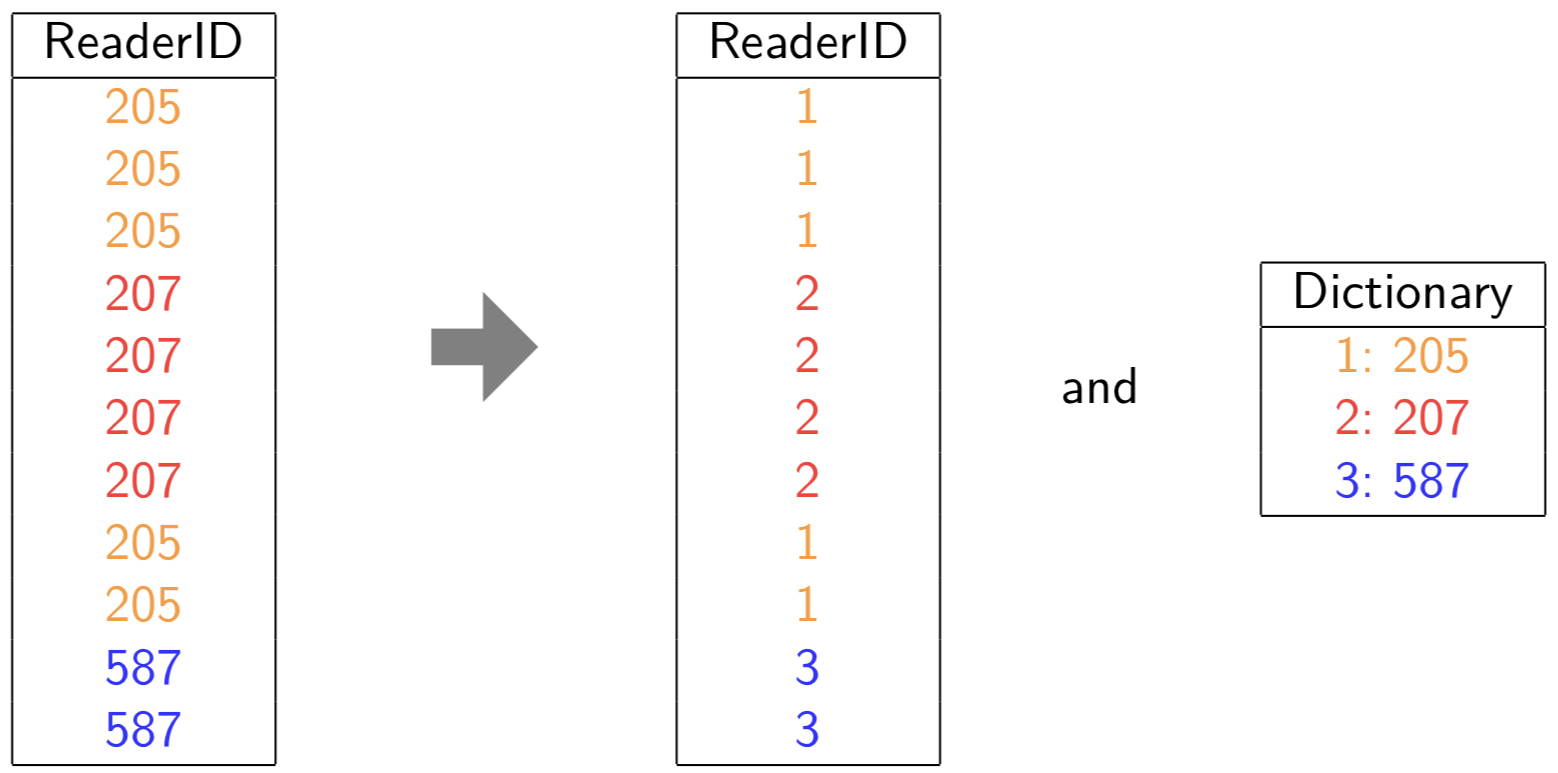
\includegraphics[width=0.50\linewidth]{images/AdvancedDataManagment/column_stores/dictionary_encoding.jpeg}
            \caption{Dictionary encoding example}
        \end{figure}
        \item In some cases, we could not only create a dictionary for single values but even for frequent sequences of values
        \begin{figure}[!hbp]
            \centering
            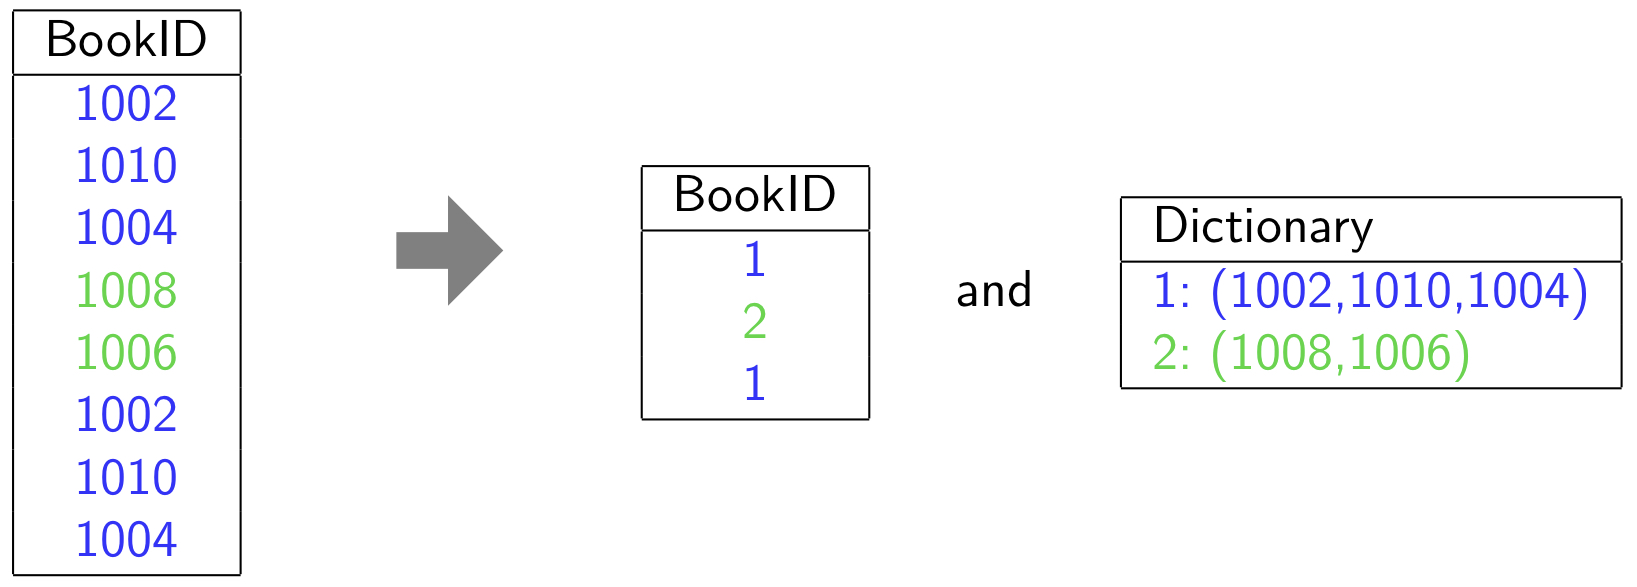
\includegraphics[width=0.40\linewidth]{images/AdvancedDataManagment/column_stores/dictionary_encoding_sequence.jpeg}
            \caption{Dictionary sequence encoding example}
        \end{figure}
    \end{itemize}
    
    
    \item \textbf{Frame of reference encoding:}
    \begin{itemize}
        \item For the range of values stored in a column, one value that lies in the middle of this range is chosen as the reference value
        \item For all other values we only store the off-set from the reference value, (smaller than the original value)
        \item \(3\) bit to store all. Interval \((-4, 4)\) so 2 bit plus the sign bit
    \end{itemize}
    
    
    \begin{figure}[!hbp]
        \centering
        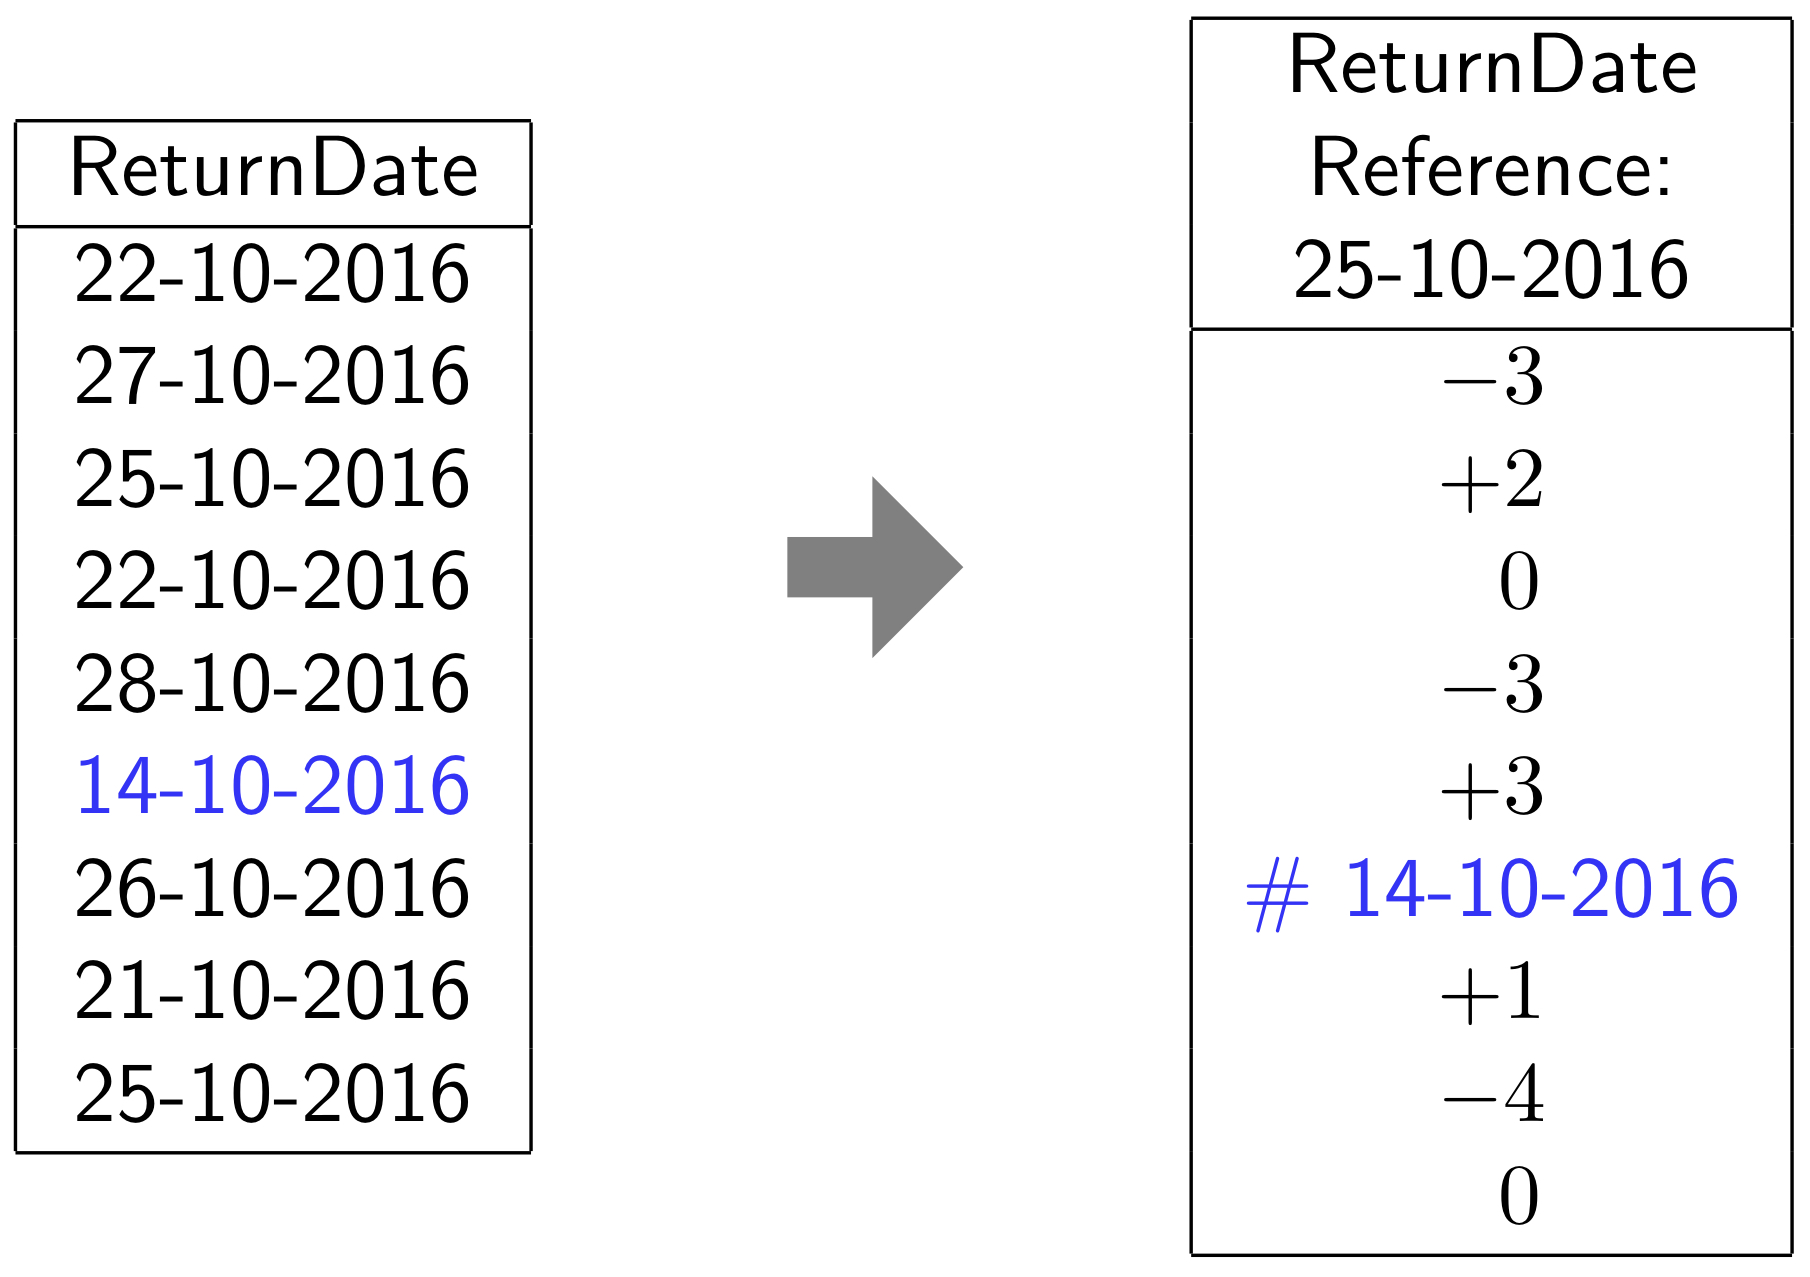
\includegraphics[width=0.60\linewidth]{images/AdvancedDataManagment/column_stores/frame_reference_encoding.jpeg}
        \caption{Frame reference encoding example}
    \end{figure}
    
    
    \item \textbf{Differential encoding:}
    \begin{itemize}
        \item An offset is stored instead of the entire value
        \item The offset is the difference between the value itself and the value in the preceding row
        \item Again the offset should not exceed a fixed size
        \item As soon as the offset gets too large, the current value is stored as an \textit{exception}
        \item This encoding is only applicable to numerical data
        \item It works best if data are stored in a sorted way
        \item In addition with each encoding we have to maintain the order inside the column as otherwise tuple reconstruction would be impossible
        
        \begin{figure}[!hbp]
            \centering
            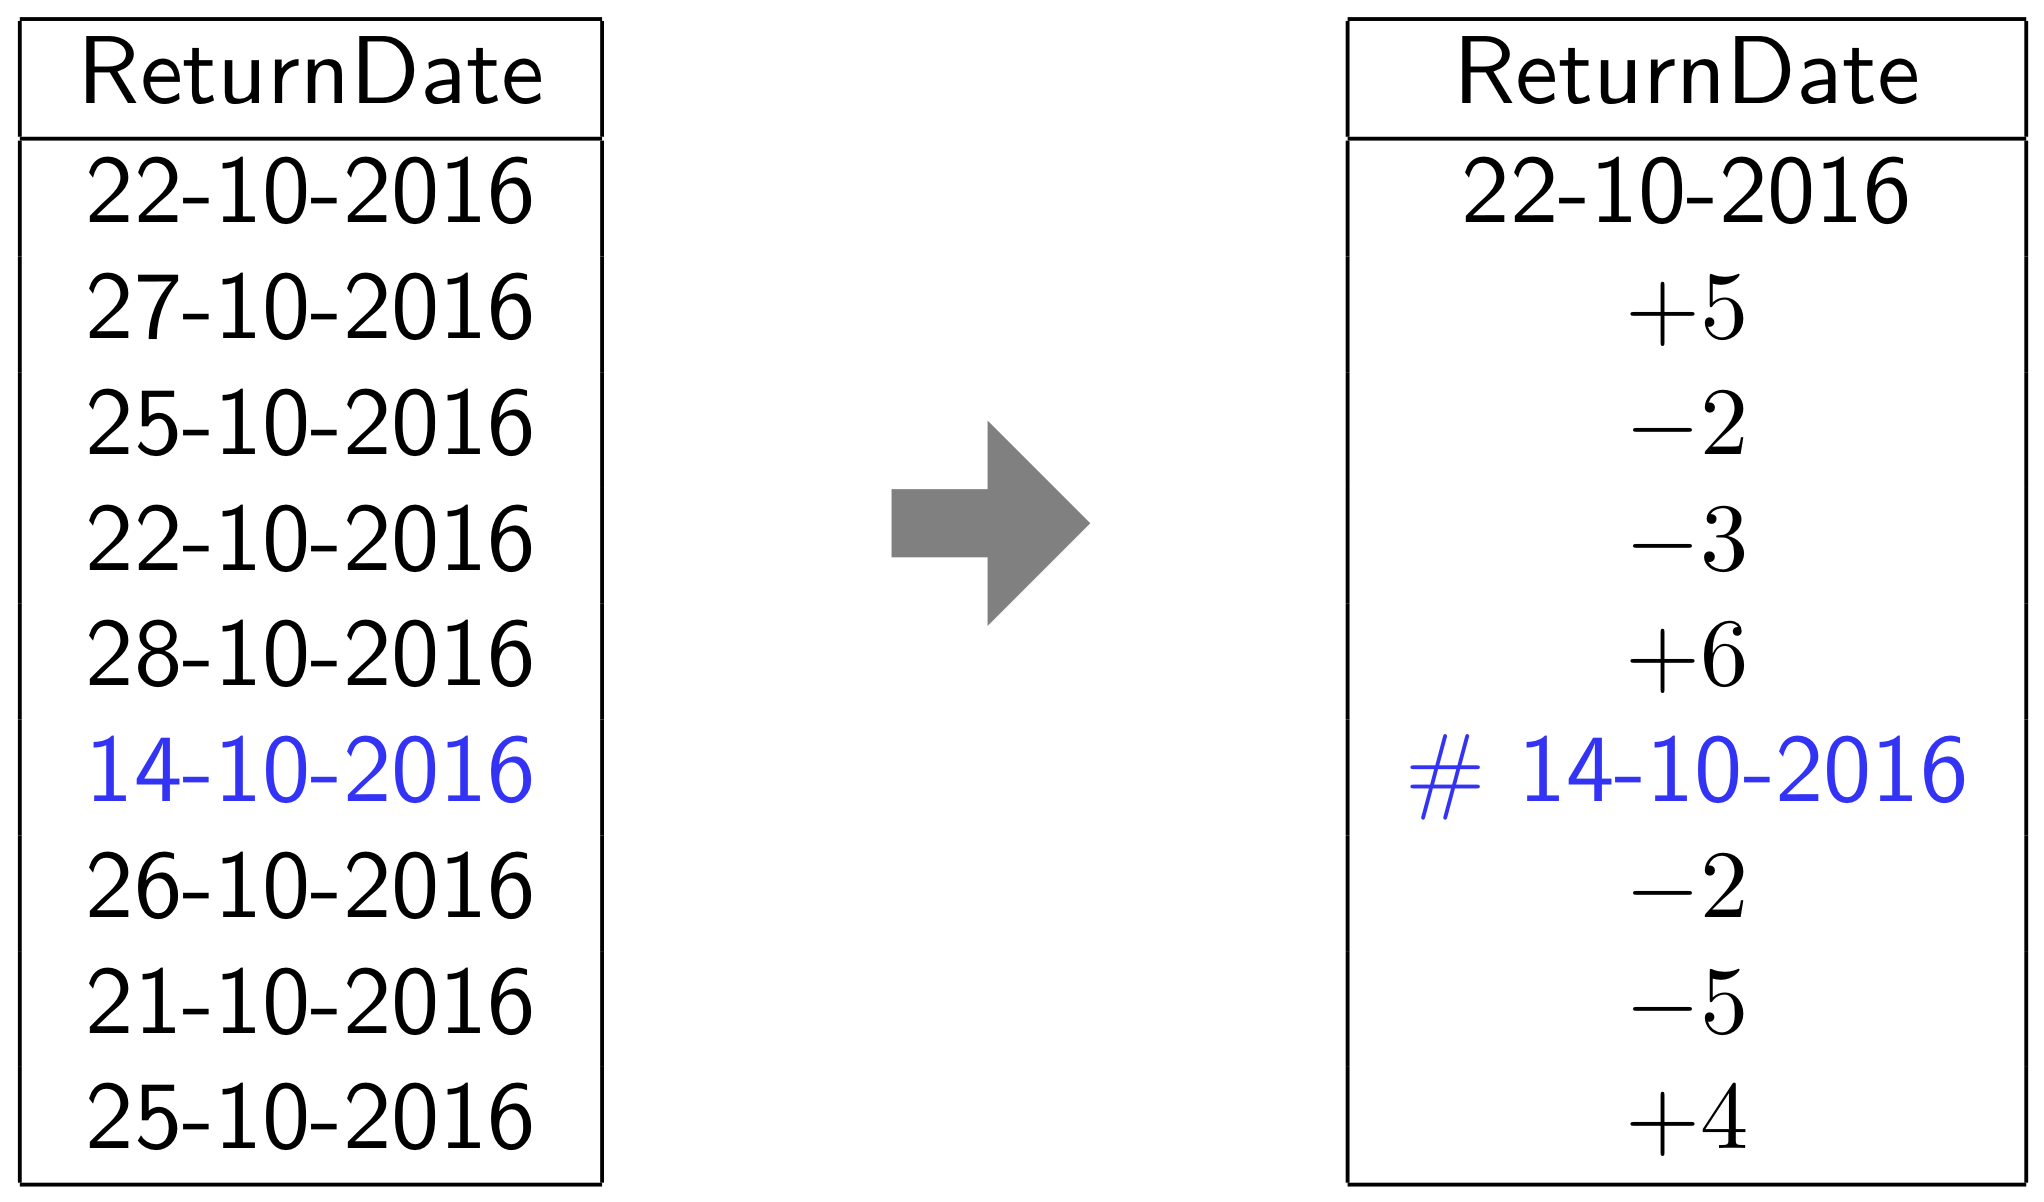
\includegraphics[width=0.60\linewidth]{images/AdvancedDataManagment/column_stores/differential_encoding.jpeg}
            \caption{Differential encoding example}
        \end{figure}
        
        \item \textbf{Disadvantages:}
        \begin{itemize}
            \item Extra runtime needed to compute the encoding
            \item Extra runtime needed to decode the data whenever we want to execute a query on them
        \end{itemize}
        \item Fortunately some queries can actually be executed on the compressed data so that no decompression step is needed. Like the following example:
        \vspace{0.3cm}
        We have that the ReaderID is encoded as a sequence as follows:
        \vspace{0.3cm}
        
        \centerline{((\textcolor{red}{205}, 1, 3), (\textcolor{orange}{207}, 4, 2), (\textcolor{red}{205}, 6, 1))}
        \vspace{0.3cm}
        Query: "How many books does each reader have?"
        \vspace{0.3cm}
        
        \centerline{SELECT ReaderID, COUNT(*) FROM BookLending GROUP BY ReaderID}
        \vspace{0.3cm}
        Now the column store does not have to decompress the column into the entire original column with 6 rows. It just returns (the sum of) the run-lengths for each ReaderID value.
        \begin{itemize}
            \item \textit{Reader 205} is 3 + 1 = 4
            \item \textit{Reader 207} is 2
        \end{itemize}
        
        \centerline{Result: \{(205, 4), (207, 2)\}}
    \end{itemize}
 \end{itemize}
 
\subsection{Null Suppression}
Sparse columns are columns that contain many NULL values. A more compact format of a sparse column can be achieved by \textbf{not storing these null values}, but some additional information is needed to distinguish the non-null columns from the null columns

\begin{itemize}
    \item \textbf{Position list:}
    \begin{itemize}
        \item List that stores only the non-null positions but discards any null values
        \item As metadata the total number of rows and the number of non-null positions are stored
    \end{itemize}
    
    
    %IMAGE
    
    
    \item \textbf{Position bit-string:}
    \begin{itemize}
        \item Bit-string for the column where non-null positions are set to 1 but null positions are set to 0
        \item Accompanied by a list of the non-null values in the order of their appearance in the column
    \end{itemize}

    %IAMGE

    \item \textbf{Position range:}
    \begin{itemize}
        \item If there are \textit{sequences of non-null values} in a column, the range of this sequence can be stored together with the list of values in the sequence
        \item As metadata the total number of rows and the number of non-null positions are stored
    \end{itemize}
\end{itemize}

\begin{tcolorbox}
These three encodings \textit{suppress nulls} and hence \textit{reduce the size of the data set}. However, internally, \textit{query evaluation} in the column store must be \textit{adapted to the null suppression} technique applied
\end{tcolorbox}

\section{Column striping}
The process of column striping decomposes a document into a set of columns:
\begin{itemize}
    \item One column for each unique path in the document
    \item For each unique path, the values coming from different documents are written to the same column in order to be able to answer analytical and aggregation queries over all documents efficiently
    \item  However we need some metadata to recombine an entire document as well as to be able to query it. These \textit{metadata} are called:
    \begin{itemize}
        \item \textit{Repetition level} to handle repetitions of paths and it denotes at which level in the path the last repetition occurred. Moreover it can range from \textbf{0} to the \textbf{path length}:
        \begin{itemize}
            \item \textbf{0:} no repetition has occurred so far
            \item \textbf{Path length:} denotes that the entire path occurred for the previous field
        \end{itemize}
        \item \textbf{Definition level} to handle non-existent paths of optional or repeated fields and it denotes the maximum level in the path for which a value exist. Only non-required fields are counted for the definition level
    \end{itemize}
\end{itemize}

\chapter{Extensible Record Stores}
%from age 285 to 313
Extensible record stores are database systems akin to \textbf{Google’s
BigTable system}.
\begin{itemize}
    \item A "Bigtable" is a sparse, distributed, persistent multi-dimensional stored map
    \item It is indexed by \textbf{row key, column key and timestamp}
    \item A \textbf{value} in the map is an uninterpreted array of bytes, also called string
    \item MAP: (row:string, column:string, time:int64) \(\leftarrow\) string
\end{itemize}
These databases have tables as their basic data structure although with a highly flexible column management; they implement the concept of \textbf{column families} that act as containers for subsets of columns.

\section{Logical Data Model}
Extensible record stores do not use the normalization paradigm from RDBMSs. Instead they encourage a certain amount of \textbf{data duplication} for the sake of \textit{better query locality} and more \textit{efficient query execution}.

While the design in the relational model is centered around entities and later on normalization, an extensible record store first of all a typical query workload should be identified and data modeled around this workload accordingly. 

What extensible record stores do to organize these key-value pairs is adding another structural dimension the \textbf{column family}:
\begin{itemize}
    \item It groups columns that are often accessed simultaneously in a typical query
    \item The columns inside are called \textbf{column qualifier}
    \item The full \textbf{column name} consists of the column family name and the column qualifier
    \item \textbf{Value} for each column in a row
    \item \textbf{Row keys} link column of the same entity. However, there is no way of specifying foreign key constraints between different column families and no referential integrity is ensured
\end{itemize}

The \textbf{advantages} of column families are the following:
\begin{itemize}
    \item They provide data locality by storing data inside a column family together on disk
    \item They provide dynamic addition of new columns (at run time)
\end{itemize}
And the following \textbf{characteristics}:
\begin{itemize}
    \item They have to be created before used
    \item Columns families are fixed for a table
    \item There can be infinitely many columns in each column family
\end{itemize}

\begin{figure}[!hbp]
    \centering
    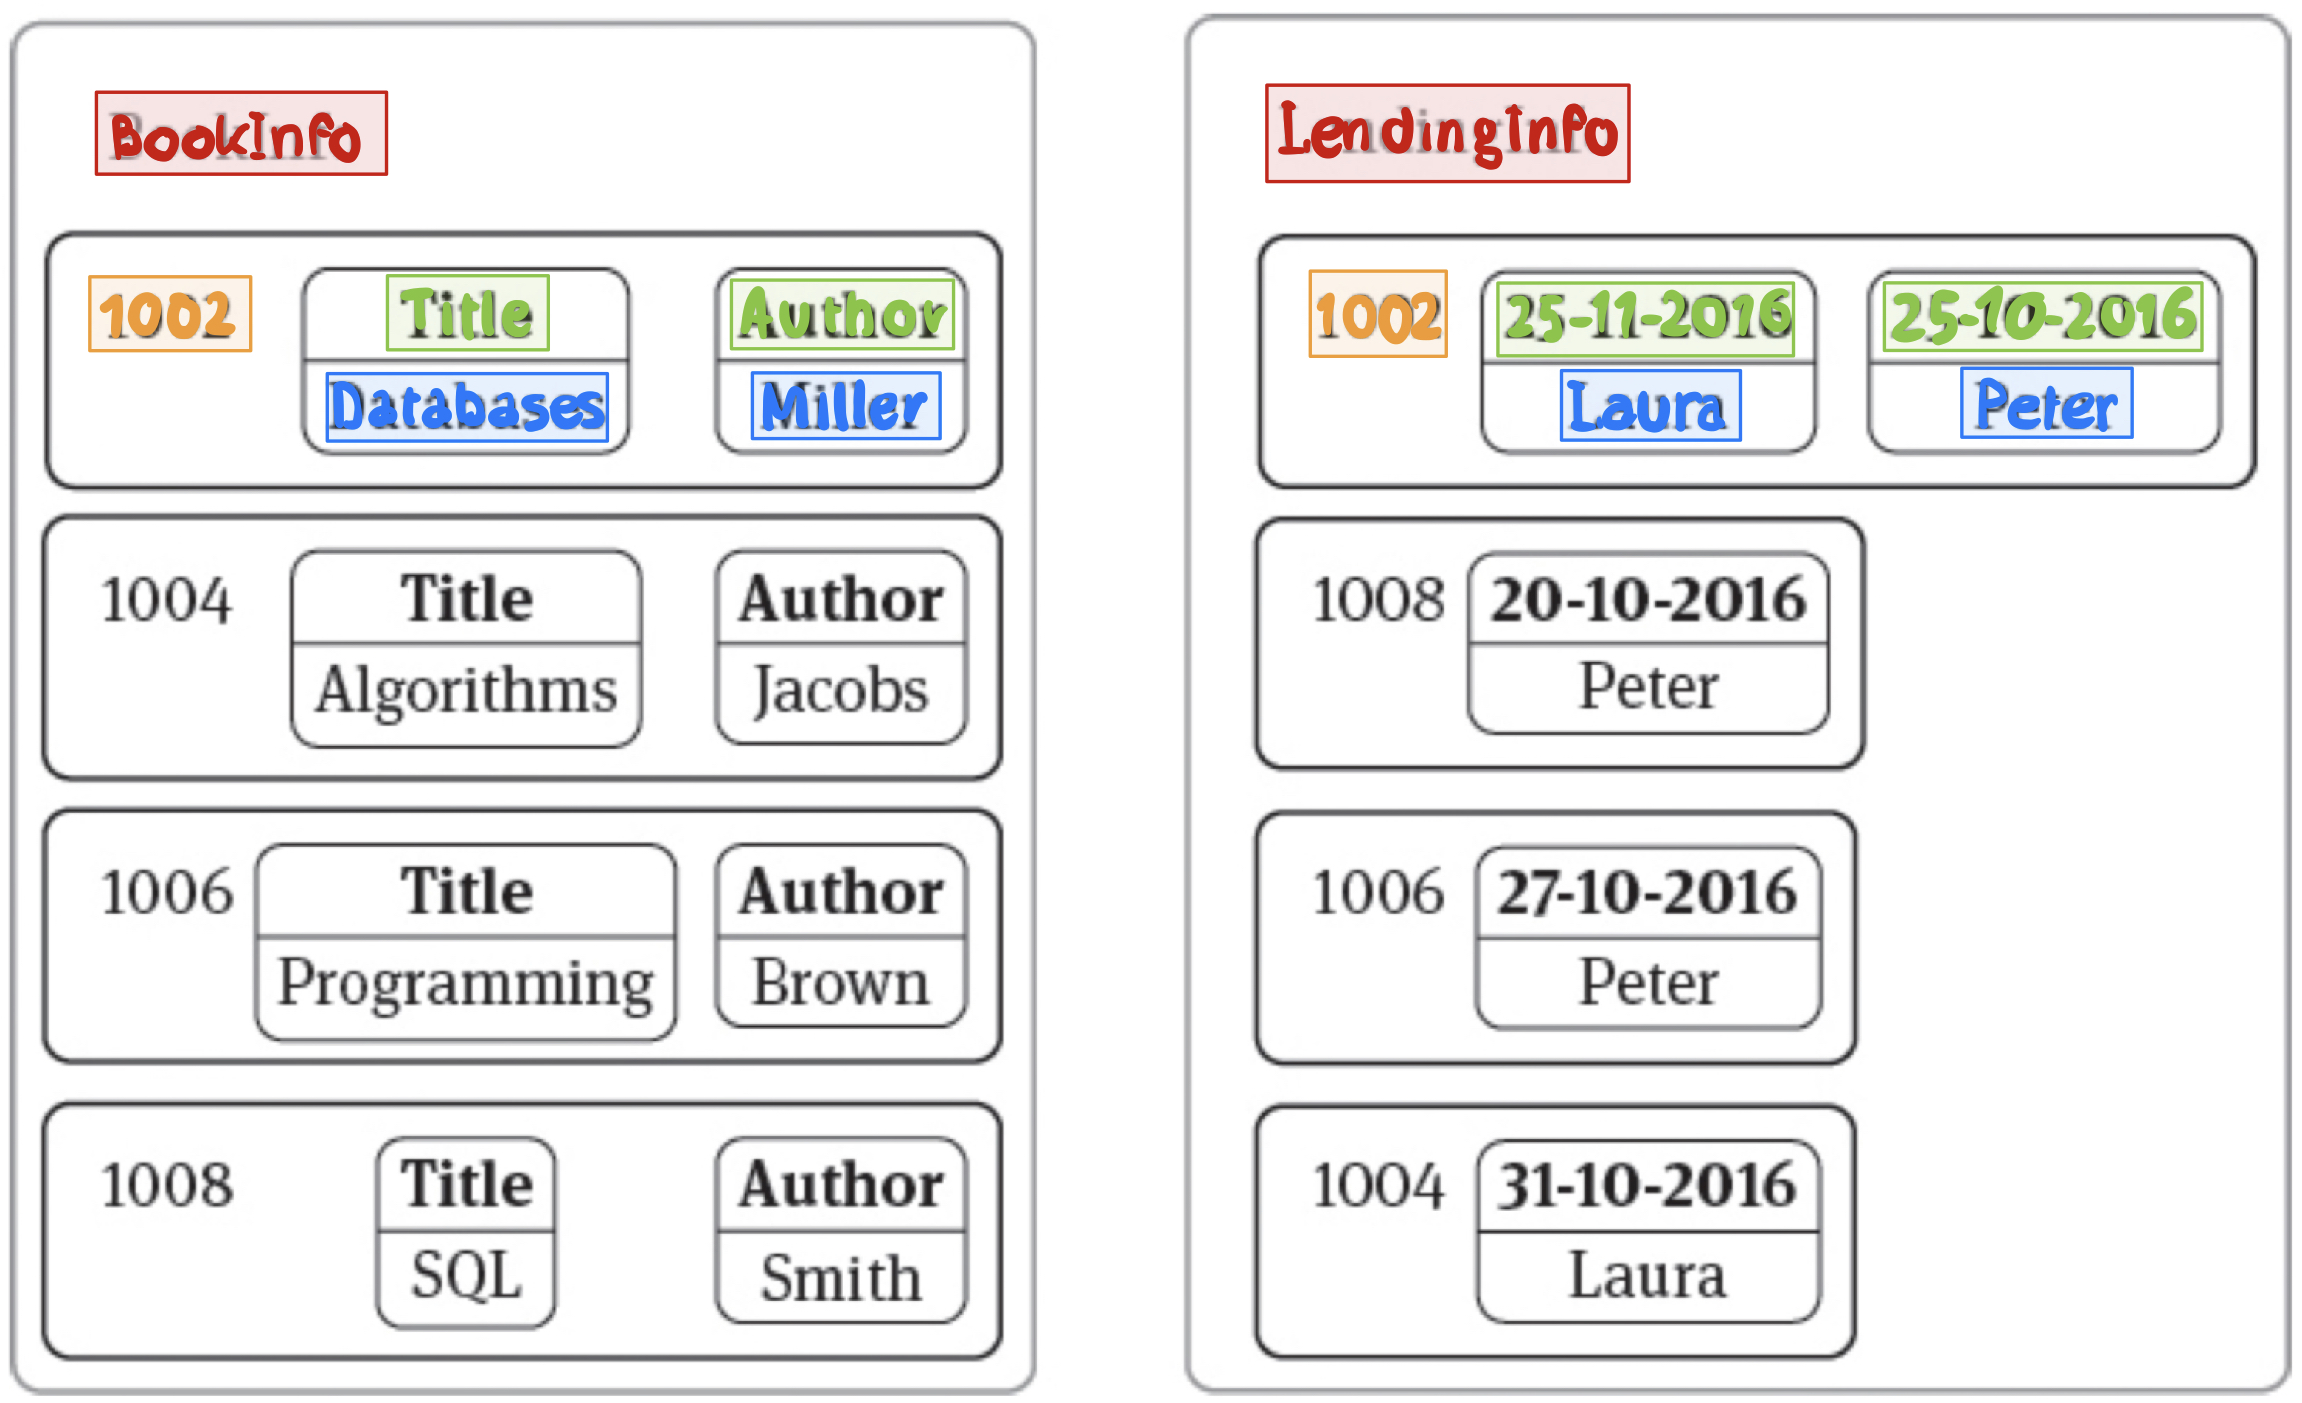
\includegraphics[width=0.90\linewidth]{images/AdvancedDataManagment/extensible_record_store/names_definition.jpeg}
    \caption{\textcolor{red}{Column Families}, \textcolor{green}{Column Qualifiers}, \textcolor{blue}{Values}, \textcolor{orange}{Row Keys}}
\end{figure}

At this point we also see the \textit{flexibility} of how columns can be added to rows, indeed one row can have different columns than other rows inside the same column family. This is why extensible record stores are good at storing \textbf{sparse data:} 
\begin{itemize}
    \item An extensible record store just \textit{ignores} values that are not present and \textit{no null values} are included in rows.
    \item The \textbf{concatenation} of \textit{row key}, \textit{column family name} and \textit{column qualifier} identifies a \textbf{cell} in the extensible record store
    \item The \textbf{full key} in order to access to a specific cell is in the form of:
    \[rowkey:columnfamily:columnqualifier\]
\end{itemize}

Extensible record stores offer the convenient feature of \textbf{ordered storage:}
\begin{itemize}
    \item While the relational data model is set-based and the order of the output basically depends on the DBMS
    \item Extensible record stores sort the data internally
    \begin{itemize}
        \item Inside a \textit{column family}, the rows are sorted by their \textbf{row keys}
        \item Inside a \textit{row} the columns are sorted by their \textbf{qualifiers}
    \end{itemize}
\end{itemize}

Other extensible record stores (like Cassandra) offer data types for row keys and column qualifiers and hence sorting can be done according to the data type and may differ from the binary order.

\begin{figure}[!hbp]
    \centering
    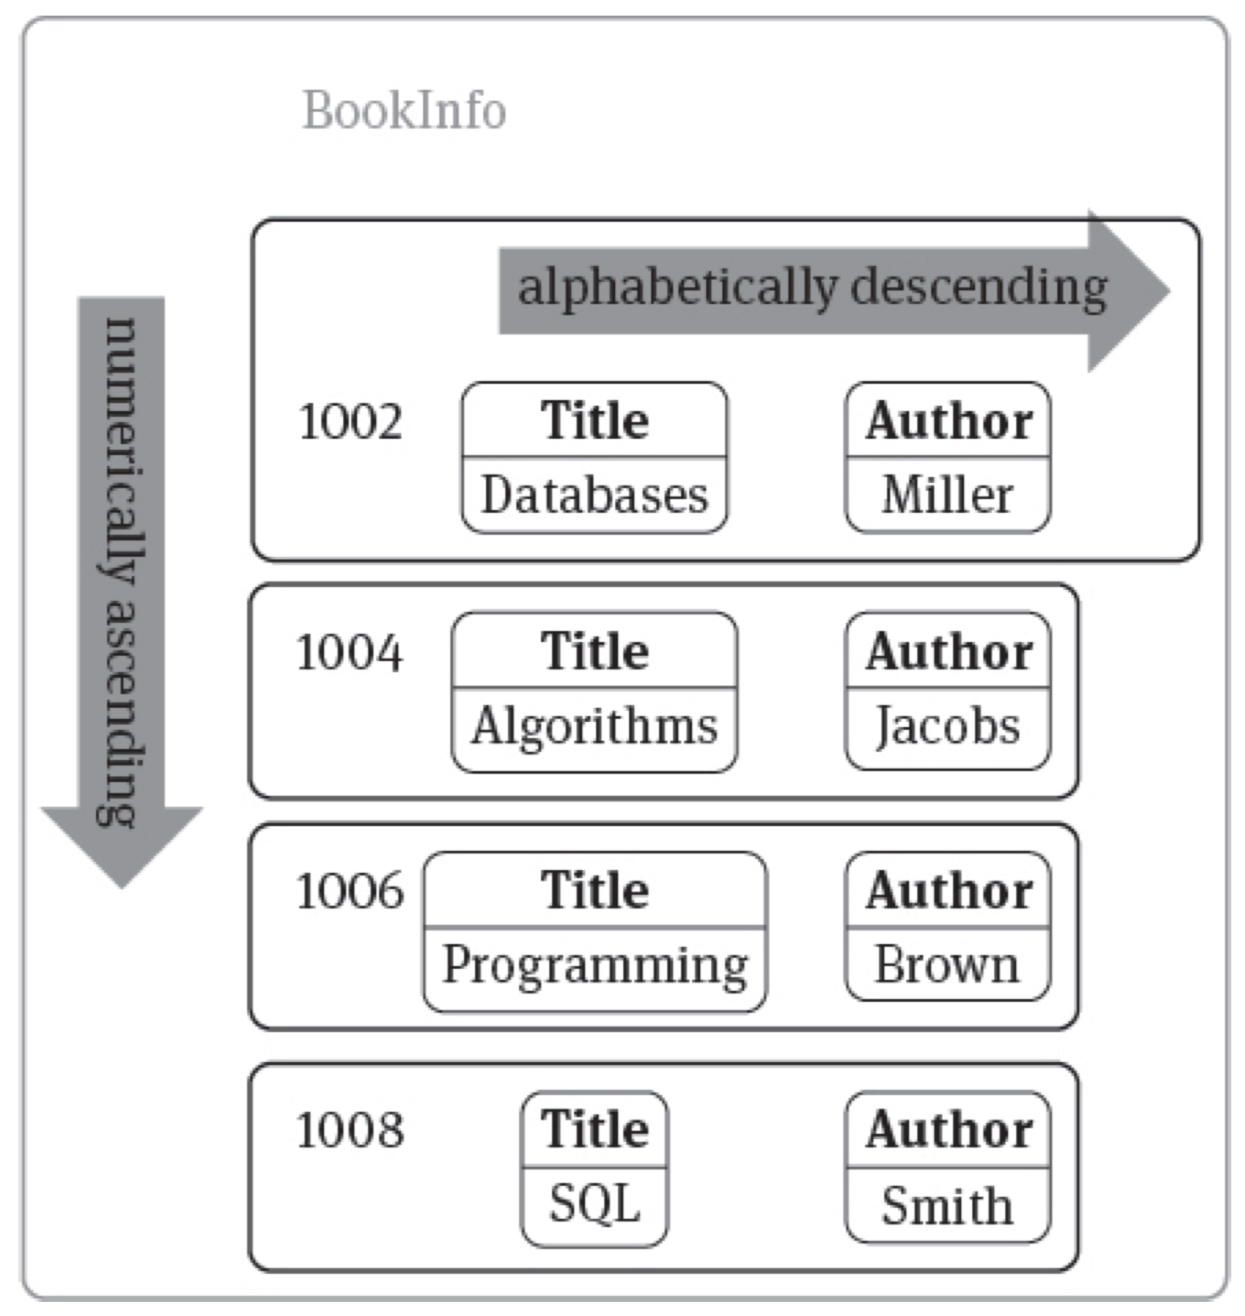
\includegraphics[width=0.50\linewidth]{images/AdvancedDataManagment/extensible_record_store/BookInfo.jpeg}
    \caption{Ordering features of BookInfo}
\end{figure}

\begin{figure}[!hbp]
    \centering
    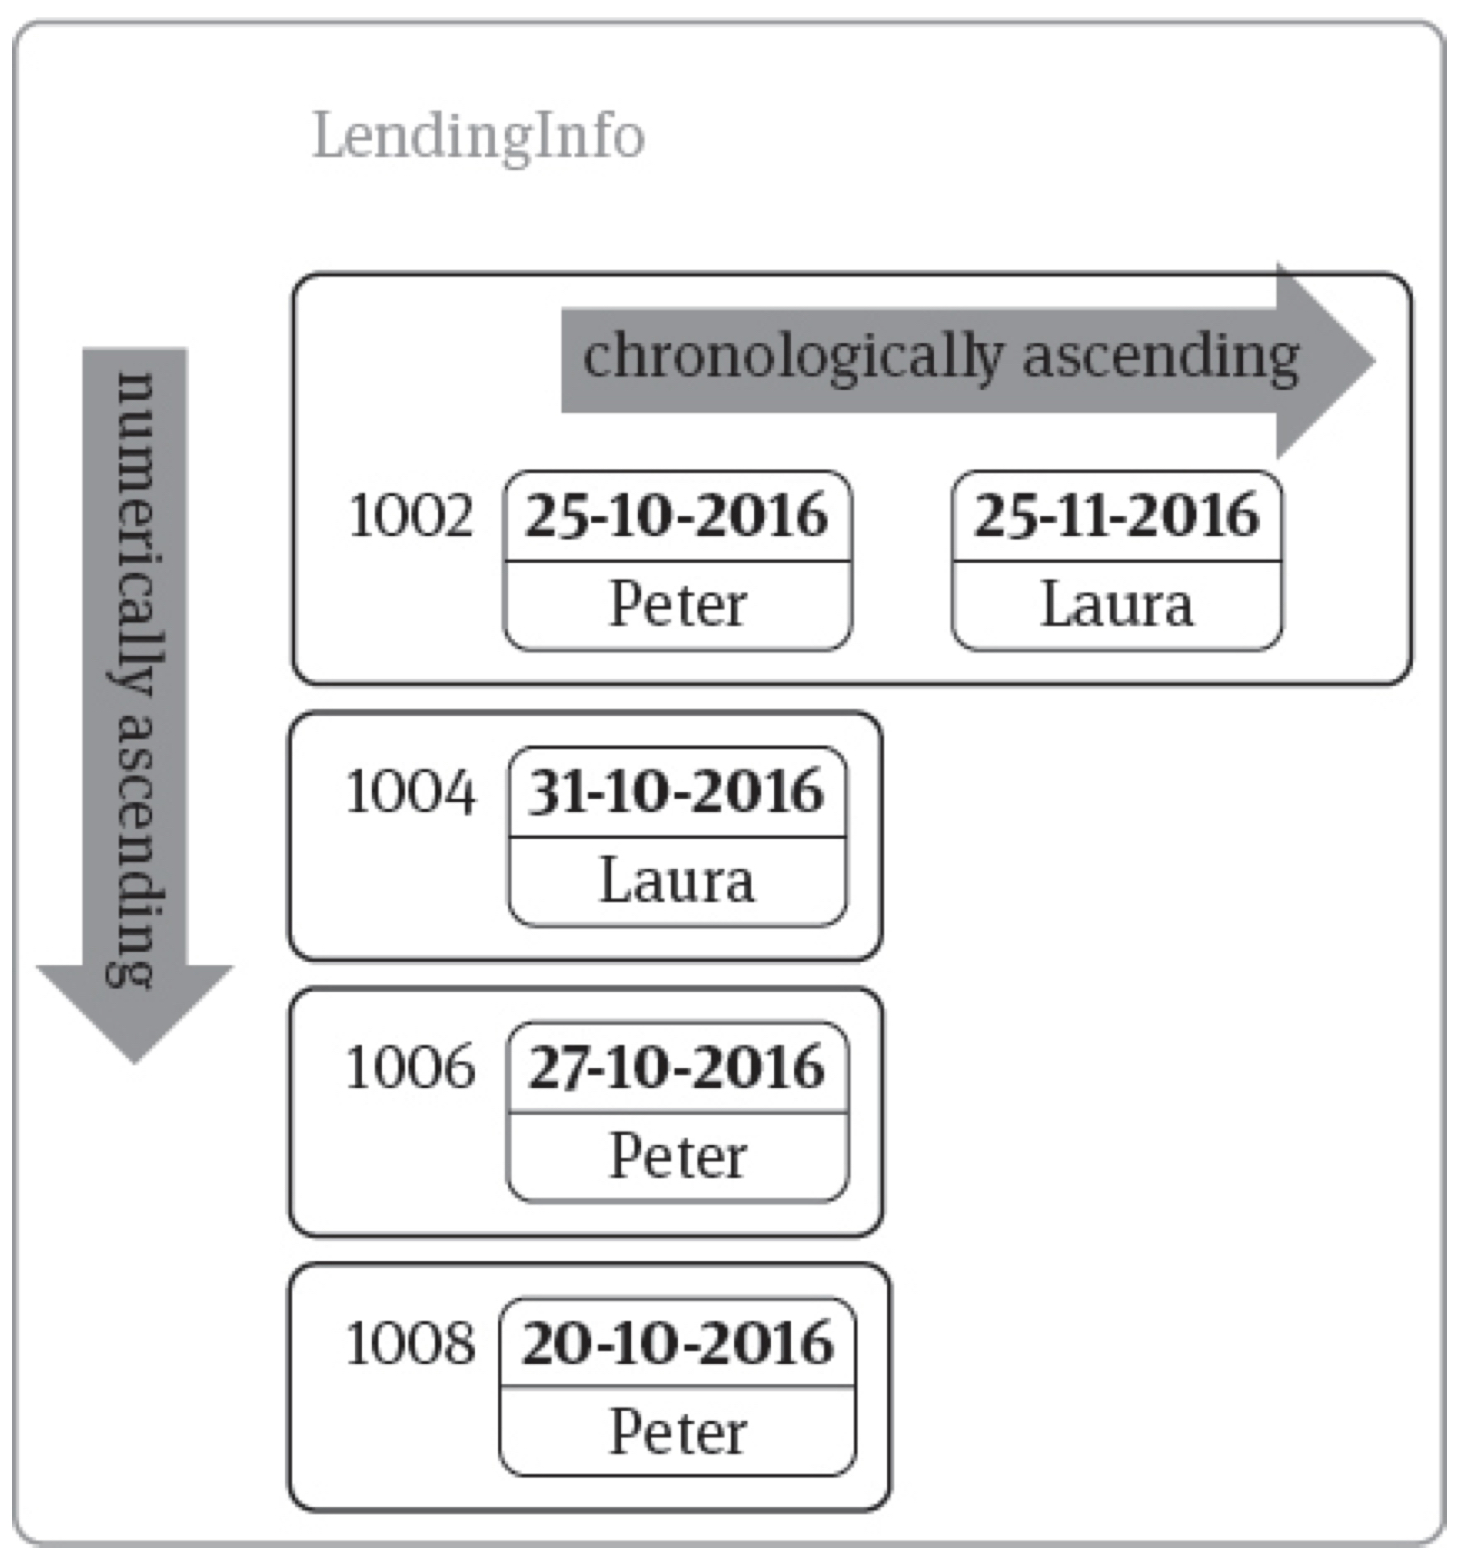
\includegraphics[width=0.50\linewidth]{images/AdvancedDataManagment/extensible_record_store/LendingInfo.jpeg}
    \caption{Ordering features of LendingInfo}
\end{figure}

\newpage
With these ordering features, extensible record stores are particularly well-suited for identifying \textbf{contiguous sequences of columns}.

\vspace{0.5cm}
\centerline{"What are the names of those readers who have to return
books on or before 31-10-2016?"}
\vspace{0.5cm}

To answer this query we have to find out what is following. The columns with column qualifiers less than or equal to 31-10-2016. But \textbf{due to the ordering} the matching columns are stored in a \textit{consecutive range} and that we do not have to search further once we have reached a column qualifier greater than 31-10-2016.

Last but not least, some extensible record stores add \textit{one more dimension} to the row-column family-column space: \textbf{time}.
\begin{itemize}
    \item Each insert or update is accompanied by a \textbf{timestamp} and it can be specified by the user
    \item Extensible record stores provide an \textbf{automatic versioning} of column values
    \item When a read command \textit{without an explicit timestamp} is issued on a cell, the \textit{most recent} version is returned
    \item Versioning can further be configured by specifying a \textit{maximum threshold} for the amount of stored version. 
    \begin{itemize}
        \item The \textbf{oldest version} will \textit{automatically be discarded} once a new version is stored and the maximum value is exceeded
    \end{itemize}
    \item Another option for \textbf{automatic discarding} is to specify a \textbf{time-to-live value} for each cell:
    \begin{itemize}
        \item When the specified time span has \textit{elapsed}, the corresponding \textit{version} of the cell is \textbf{deleted}
    \end{itemize}
\end{itemize}

Furthermore, extensible record stores usually do not make a distinction between inserts and updates. Instead, a
\textbf{put command} is provided that checks whether there is an existing cell for the given key:
\begin{itemize}
    \item If there is, the \textit{value} for the key will be \textbf{updated}
    \item Otherwise a \textit{new cell} is \textbf{inserted}
\end{itemize}
This is why this operation is sometimes called an \textbf{upsert}.

\section{Physical storage}
Extensible record stores use several techniques for \textbf{efficient query answering and recovery.}

\subsection{Memtables and immutable sorted data files}
\subsubsection{Writing to memory tables and data files}
Extensible record stores implement a \textit{write-optimized storage model}
\begin{itemize}
    \item All data records written to the on-disk store will only be appended to the existing records
    \item Once written, these records are read-only and cannot be modified, they are \textbf{immutable}
    \item Any modification must be simulated by appending a new record in the store
\end{itemize}


\begin{figure}[!h]
    \centering
    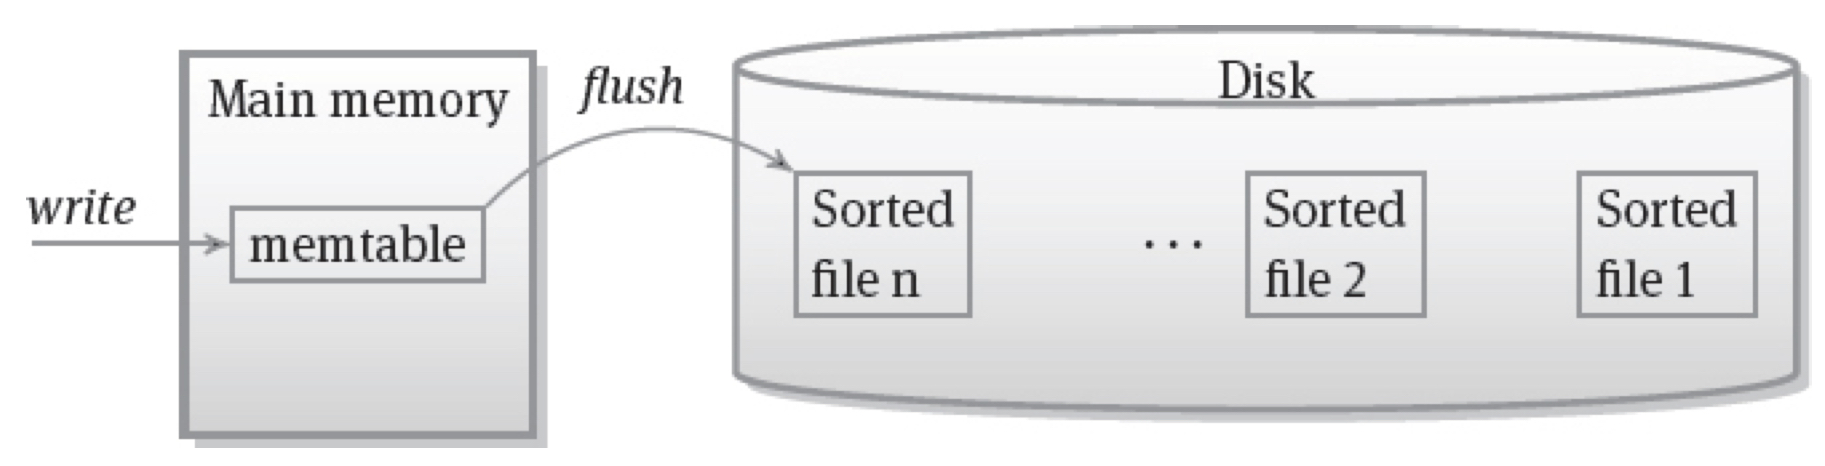
\includegraphics[width=0.70\linewidth]{images/AdvancedDataManagment/extensible_record_store/writing.jpeg}
    \caption{Writing to memory tables and data files}
\end{figure}

\subsubsection{Reading to memory tables and data files}
There are two types of read requests:
\begin{itemize}
    \item \textit{Get} also called \textbf{point query}. It accesses a particular row (identified by its row key).
    \item \textit{Scan} also called \textbf{range query}. It iterates over a contiguous range of rows depending on some condition on the row key.
\end{itemize}
\begin{figure}[!h]
    \centering
    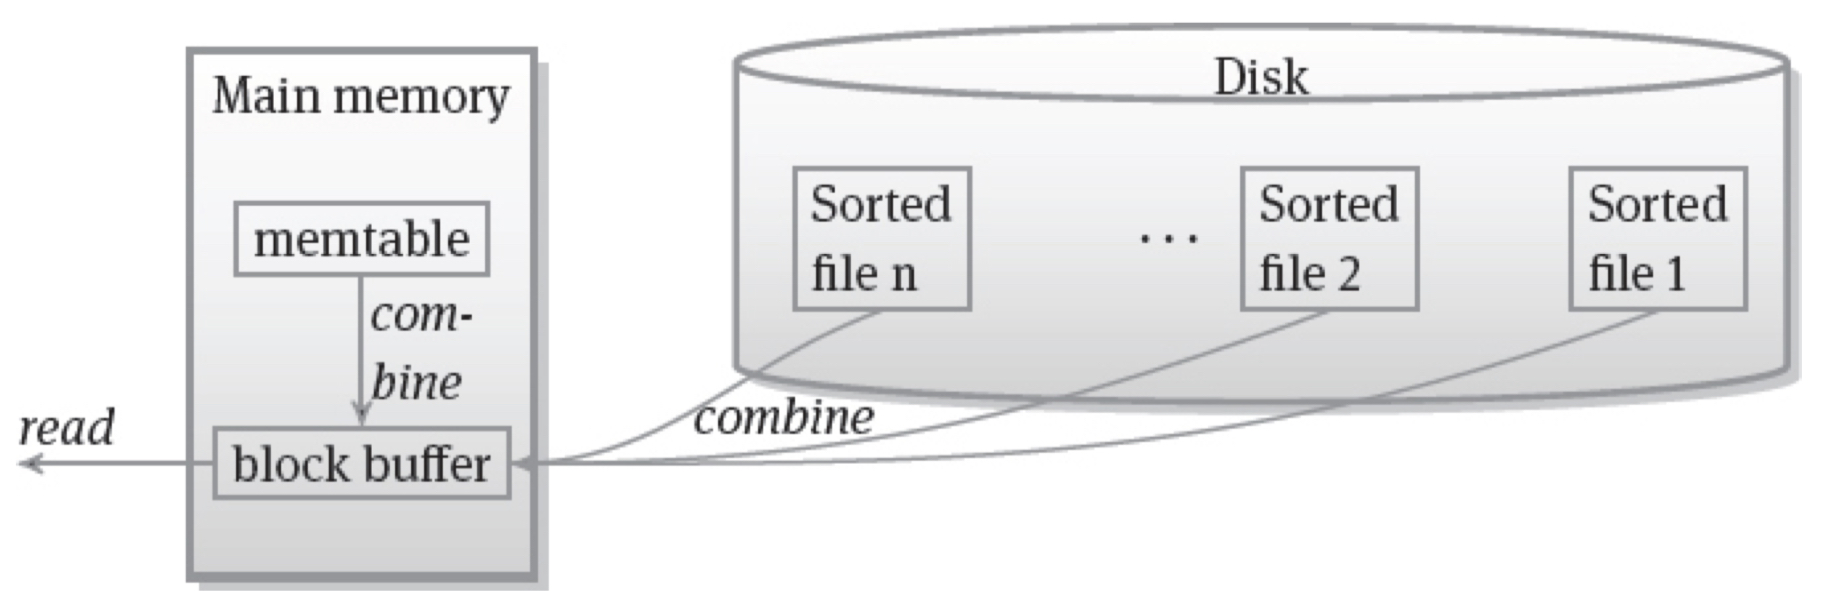
\includegraphics[width=0.70\linewidth]{images/AdvancedDataManagment/extensible_record_store/reading.jpeg}
    \caption{Reading to memory tables and data files}
\end{figure}


\newpage
\subsubsection{Consideration of both Reading and Writing operations}
More specifically, \textit{writing to} and \textit{reading from} an extensible record store comprises the following steps:
\begin{itemize}
    \item \textbf{Memtable:} 
    \begin{itemize}
        \item The most recent writes are collected in a main memory table of fixed size
        \item Usually there is one memtable per column family
        \item A record in the memtable is identified by its key (row key, column family, column qualifier and timestamp in milliseconds)
        \item Timestamp can be chosen by the user
        \item If no particular timestamp is specified in the put request, the current system time is used by default
    \end{itemize}
    \item \textbf{Tombstones:} 
    \begin{itemize}
        \item Deletions are treated by writing a new record for a key
        \item This record has no value assigned to it; instead a \textit{delete marker} (called \textbf{tombstone}) is attached to the record
        \item The tombstone masks all previous versions which will then be \textit{invisible to the user}
        \item A tombstone can for example \textbf{mark as deleted} either a \textit{single version of a column} or an \textit{entire column family}
    \end{itemize}
    \item \textbf{Sorted data files:} 
    \begin{itemize}
        \item Once the memtable is filled, it is written to disk (\textbf{flushed}) and an entirely new memtable is started. With this action its records are sorted by key
        \item The flushed sorted data files on disk are \textbf{immutable}
        \item The \textbf{advantage of immutable data files} is that \textit{buffer management} is a lot \textit{easier}: no dirty pages
    \end{itemize}
    \item \textbf{Combine upon read:} 
    \begin{itemize}
        \item The \textbf{downside} of immutable data files is that they \textbf{complicate the read process}
        \item Retrieving all the relevant data that match a user query requires combining records from several on-disk data files and the memtable
    \end{itemize}
\end{itemize}


Once the row keys to be accessed are identified, the result can be restricted to a subset of the columns inside each row. In some extensible record stores a set of versions of a cell can also be accessed. Usually, a \textit{range of timestamps} can also be specified in a per-query basis;

Combining records from various on-disk data files and the memtable and identifying the most recent version of a column is \textit{not trivial}, there may be a clash of timestamps.
\begin{itemize}
    \item If the user specifies a key that already exists in a data file, a new record with the same key is appended to the memtable and later on flushed to a new data file
    \item When reading this key, several values for exactly the same key could be returned from different data files
    \item Desirable to determine a unique most recent value for each key
    \item \textbf{Unique sequence number} of the stored data files:
    \begin{itemize}
        \item The record for a key that is contained in the data file with the highest sequence number is the most recently written one
    \end{itemize}
    \item Additional difficulty comes since the extensible record store has to \textit{interpret} the \textbf{time-to-live (TTL)} values of records as well as \textbf{tombstones} when retrieving and combining data from multiple sorted data files
\end{itemize}
Some \textit{extra information} can be maintained for each data file to speed up the combine process; for example, the \textbf{range of row keys} in the file or the \textbf{minimum and maximum timestamp} can be stored as metadata of the file.


\subsection{File format}
Extensible records stores store the data in the on-disk data files in a certain format with the following properties:
\begin{itemize}
    \item \textbf{Data blocks:}
    \begin{itemize}
        \item An on-disk data file is composed of several data blocks
        \item In some extensible record stores, a different block size can be used in each column family and hence the block size can be specified by the user when creating the column family
        \item A block may also span multiple conventional memory pages (fixed size by the memory buffer and the OS)
        \item Memory management is even more flexible in extensible record stores
    \end{itemize}
    \item \textbf{Key-value pairs:}
    \begin{itemize}
        \item A data block may contain one or more key-value pairs
        \item Each key-value pair contains the entire key
        \item This format hence is the foundation for the flexibility of extensible record stores because no fixed database schema is needed to interpret the data
        \item This flexibility however comes at the price of \textit{repetitious occurrences} of portions of keys
        \begin{itemize}
            \item Row consists of several columns
            \item Row key is contained in every record for each of these columns
            \item Column families and column qualifiers are usually parts of keys in several different records
        \end{itemize}
        \item The \textbf{key} is followed by the \textbf{type} information, it determines if the record is a put (\textit{upsert}) in which case a new value is appended or if it is a \textit{deletion}
    \end{itemize}
    \item \textbf{Index:}
    \begin{itemize}
        \item Data files usually contain records for several keys and may become quite large
        \item \textit{Reading} records in a data file sequentially is a very inefficient method when searching for a single record for a given key in such a large data file
        \item To \textbf{speed up} the process an index structure is maintained at the end of each file
        \item The first row key on each block is inserted in the index
        \item When searching for a given key in a data file, first of all the entire index of the data file is loaded into main memory
        \item As not all row keys are maintained in the index, the index has to return either the entry for the exact search, or the index entry for the largest row key preceding the search key
        \item In the later case the exact search key is not found in the index and we hence cannot be sure whether a record for the search key is contained in the data file or not
    \end{itemize}
    \item \textbf{Trailer:} as the last component of a data file, a trailer contains management information, like where the index starts
    
    \begin{figure}[!hbp]
    \centering
    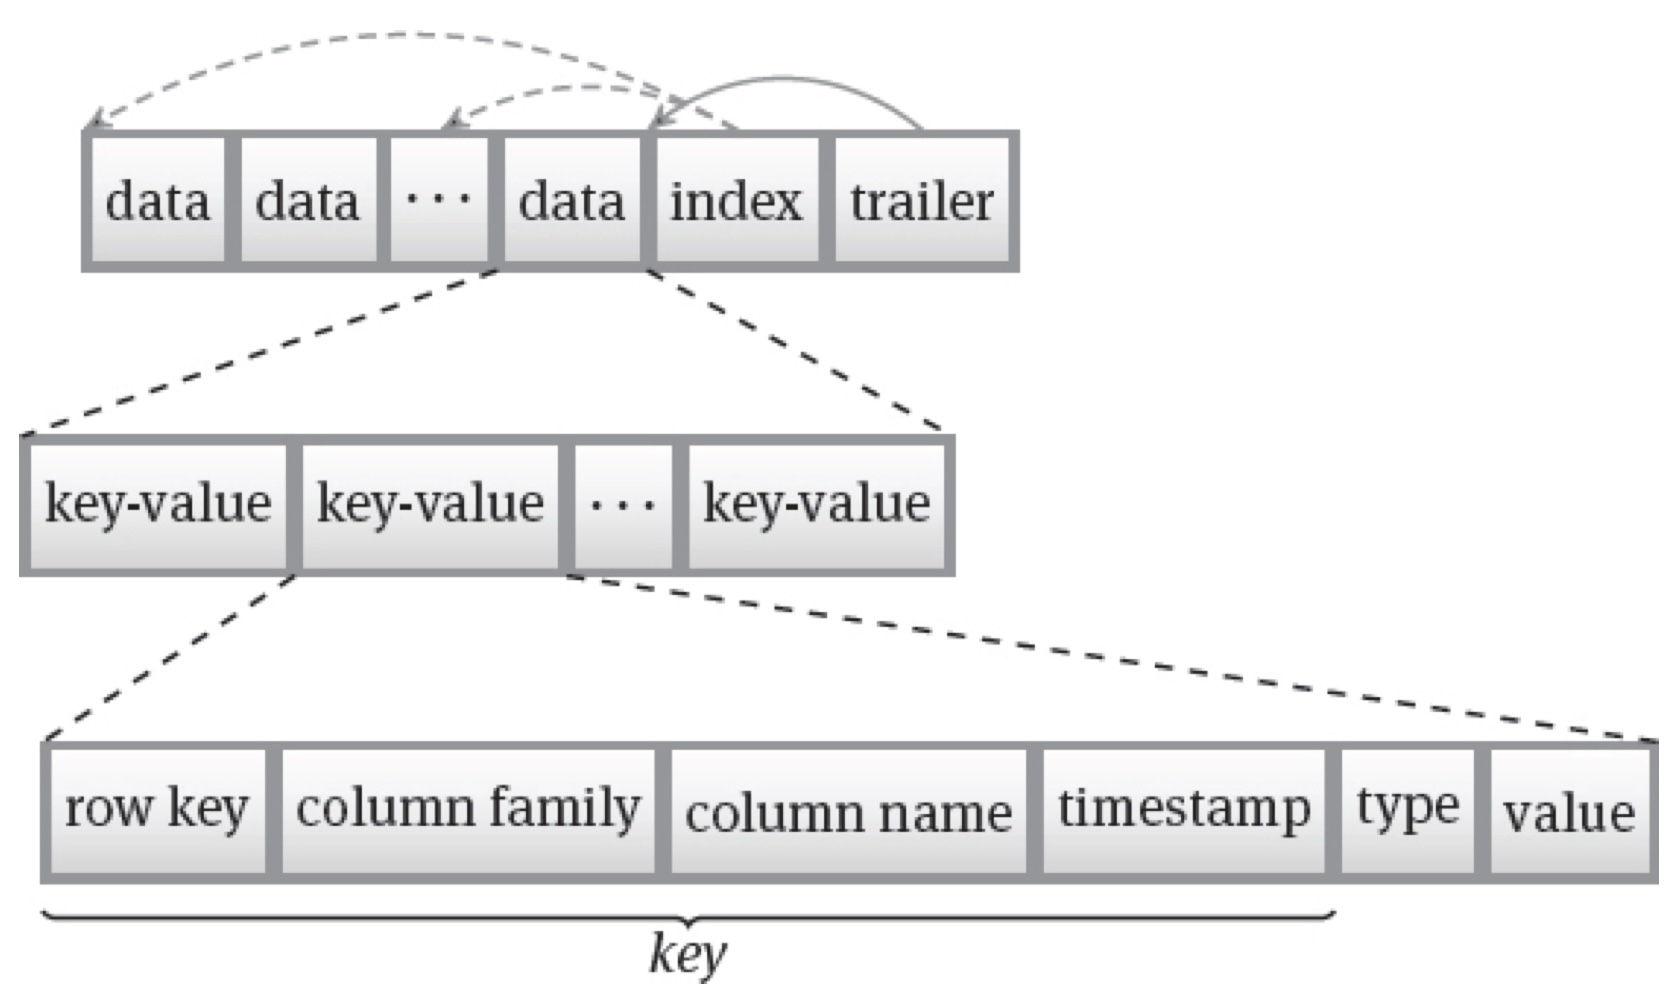
\includegraphics[width=0.50\linewidth]{images/AdvancedDataManagment/extensible_record_store/file_format.jpeg}
    \caption{File format of data files}
\end{figure}
    
    \item \textbf{Multi-level index:}
    \begin{itemize}
        \item Even though indexing is done at the block level and hence not all row keys are maintained in the index, the single index at the end of each data file might become quite large
        \item Might slow down the read process because the entire index has to be loaded into main memory before accessing any key-value pairs
        \item A multilevel index \textbf{splits the single index} into several \textit{sub-indexes}:
        \begin{itemize}
            \item One sub-index (\textit{leaf index}) is stored at the end of each block
            \item Only a small super-index (\textit{root index})  pointing to the sub-indexes is stored at the end of the data file
        \end{itemize}
    \end{itemize}
\end{itemize}

\section{Redo Logging}
\begin{itemize}
    \item The memtable is kept in volatile memory until it is eventually flushed to disk
    \item Data are only durable when stored in the on-disk data files and hence data that are contained in the memtable are vulnerable to failures of the database server
    \item \textbf{For example:} a crash of the server may wipe out the entire memory, or write errors may occur when flushing the memtable to disk
    \item When restarting the server the data in the memtable have to be recovered
\end{itemize}
\textbf{Recovery} is achieved with the help of an on-disk log file that keeps track of all records that are appended to the memtable but have not yet been flushed to the disk. This means that all data have be \textit{written twice} (log file and memtable).
\begin{itemize}
    \item Inside the log file, each record received a log sequence number (\textbf{LSN}) that maintains the \textit{chronological order} of write operations
    \item Since the data is stored to the \textit{on-disk log file} before appending them to the memtable, this process is called \textbf{write-ahead logging}
\end{itemize}

\begin{figure}[!hbp]
    \centering
    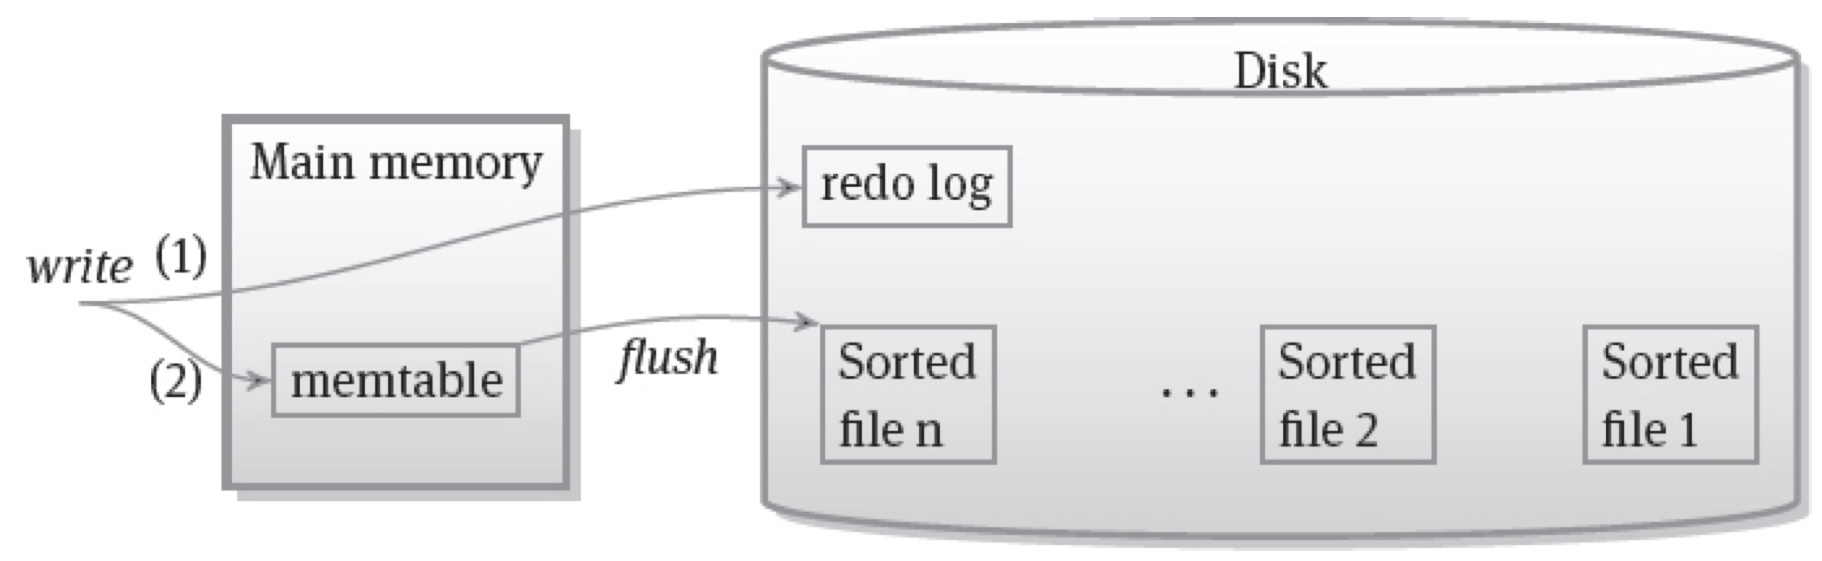
\includegraphics[width=0.70\linewidth]{images/AdvancedDataManagment/extensible_record_store/write_ahead_logging.jpeg}
    \caption{Write ahead log on disk}
\end{figure}

One peculiarity of extensible record stores is that they assume \textbf{redo-logging} to be \textit{sufficient}:
\begin{itemize}
    \item  When restarting the database server after a failure the memtable is reconstructed from the log file by re-executing all the operations in the log as ordered by their LSNs.
    \item Remarking the fact that extensible record stores do not support transactions and long-lived transaction
\end{itemize}
Although the logging mechanism \textbf{adds an additional overhead} to the write process, it in fact \textbf{improves overall write performance}: while appending a record to the log file in \textit{chronological order} is fast, sorting the records by key is \textit{slower} and can be deferred until flushing the memtable.

Last but not least, writes to the same key can be melted (fuso) and only the most recent record has to be flushed to disk. In particular, \textbf{no record} for a key must be \textbf{written} to disk at all if an \textit{upsert} for the key is \textit{masked} by a \textbf{tombstone} for the key in the memtable.


\subsection{Compaction}
After some time, several flushes of memtables will have occurred and hence there will be quite a lot of data files stored on disk, in which probably contain some outdated records:
\begin{itemize}
    \item Records whose time-to-live value has passed
    \item Records for which more recent versions exist
    \item Records for which the maximum numbe r of stored versions is exceeded
    \item Records which are masked by a tombstone
\end{itemize}
All this kind of data \textit{slow down read} processes because they have to be loaded and compared with other records in the combine process of data retrieval. This is why a process called \textbf{compaction} was devised to remove any unwanted records and merge a set of data files into a new one.

\begin{figure}[!hbp]
    \centering
    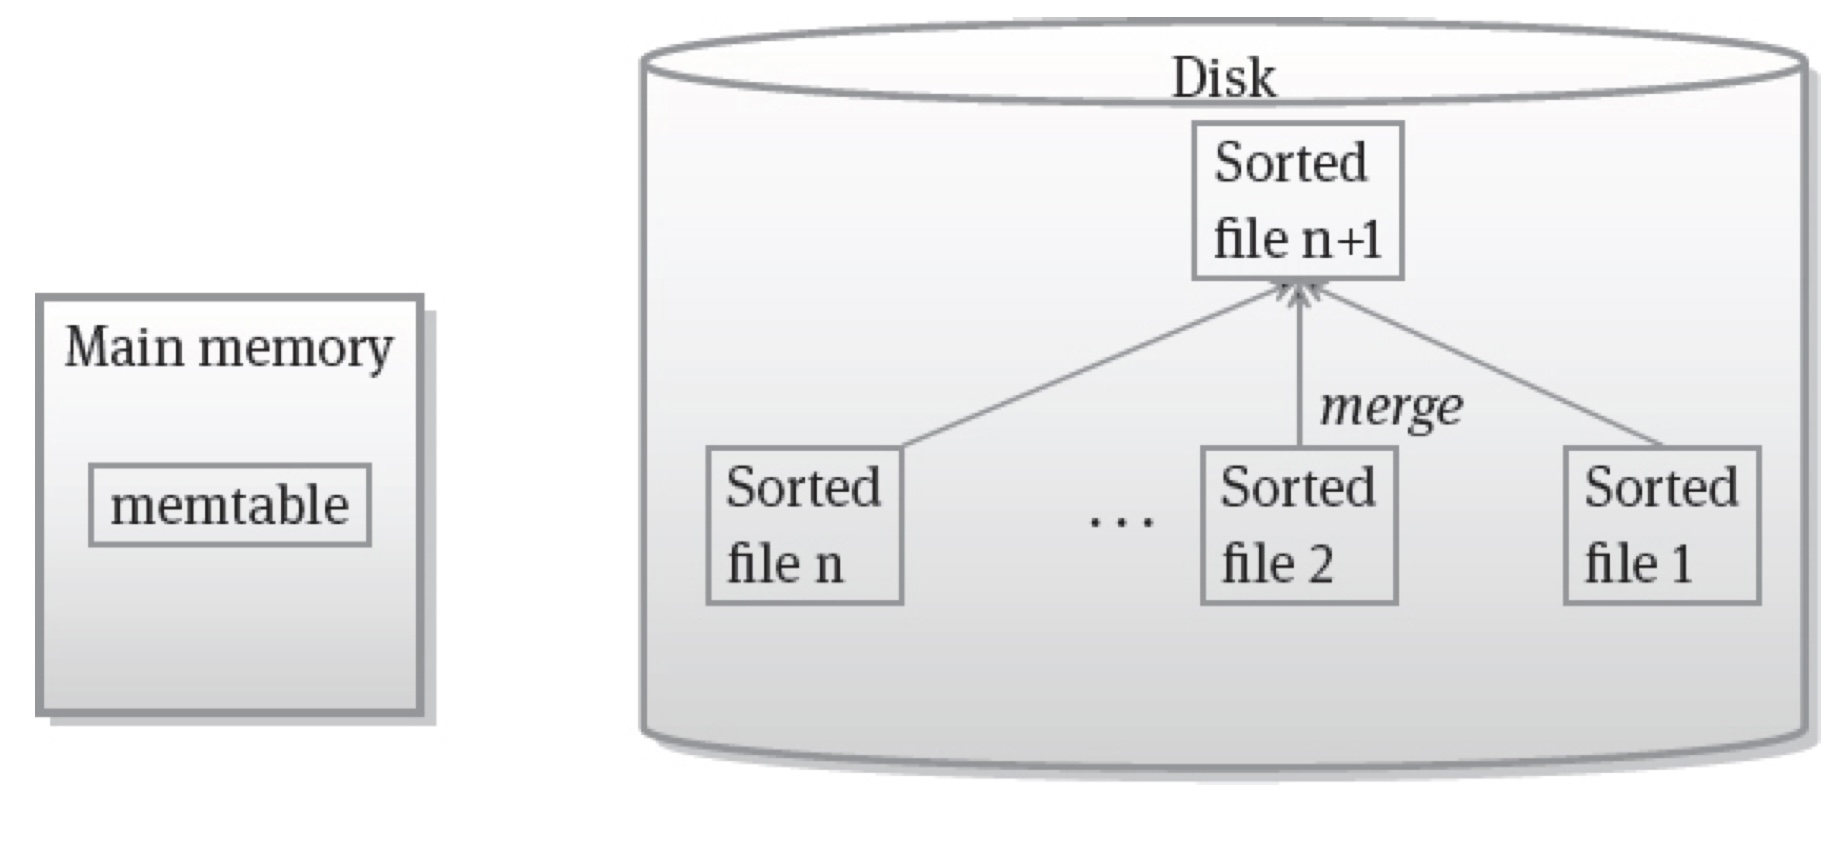
\includegraphics[width=0.70\linewidth]{images/AdvancedDataManagment/extensible_record_store/comapct.jpeg}
    \caption{Compaction on disk}
\end{figure}

In this example image a set of data file is chosen for compaction, so their records are merged and the result is written to a new larger data file.
\begin{itemize}
    \item \textbf{Minor compaction:} merges only a small subset of all data files
    \item \textbf{Major compaction:} merges all data files into a single new one
\end{itemize}
Several things have to be considered during compaction:
\begin{itemize}
    \item Records have to be sorted by key thus the index have to be reconstructed
    \item Time-to-live values have to be interpreted to ignore invalid records
    \item If a tombstone is in a data file, all file marked by it and those written before the arrival of the tombstone can be ignored
    \begin{itemize}
        \item Records that are masked by the tombstone but have been \textit{written after} the insertion of the tombstone are \textit{handled differently}: they are merged into the new data file but they still be masked by the tombstone if it is a \textit{minor compaction}
        \item \textbf{Tombstones} themselves can only be \textit{deleted} during \textbf{major compaction}
        \item So only after a major compaction more recent records for a key will be visible because they would previously be masked by the tombstone
    \end{itemize}
    \item In some extensible record stores, \textit{versioning settings} are also enforced during compaction: only a specified amount of versions for each key is kept at the maximum
    \item \textbf{Changing column family} settings can be done during \textit{major compaction}
\end{itemize}
Compaction is demanding with respect to disk space. While the compaction process is running twice the disk space as occupied by the smaller data files. However they will be discarded after compaction effectively releasing the disk space.

Several \textbf{heuristics} can be applied when choosing data files \textbf{for minor compaction:}
\begin{itemize}
    \item \textbf{Oldest files first:} chronologically ordered data file in which the oldest files with the lowest sequence number are chosen for compaction
    \item \textbf{Small files first:} to obtain a \textit{homogeneous set} of data files, several similar sized smaller files are merged into one larger file
    \item \textbf{Compaction threshold:} the user can configure a minimum number of files for which a compaction is run
\end{itemize}
Note that with these heuristics, the same record may be chosen for minor compaction several times and the records unnecessarily often migrates from smaller files into larger files.

Furthermore, the \textbf{size of the resulting compacted} files \textit{cannot be controlled}. To avoid this, \textbf{leveled compaction} has been developed:
\begin{itemize}
    \item Data files are organized into levels
    \item Data files in lower levels are smaller than data files in higher levels
    \item A \textbf{flush} always moves the memtable to a data file in the \textit{lowest level L0}
    \item \textit{Subsequent compaction} steps move a record only from one level to the next, so amount of merges for each record is bounded by the number of levels
\end{itemize}

\begin{figure}[!hbp]
    \centering
    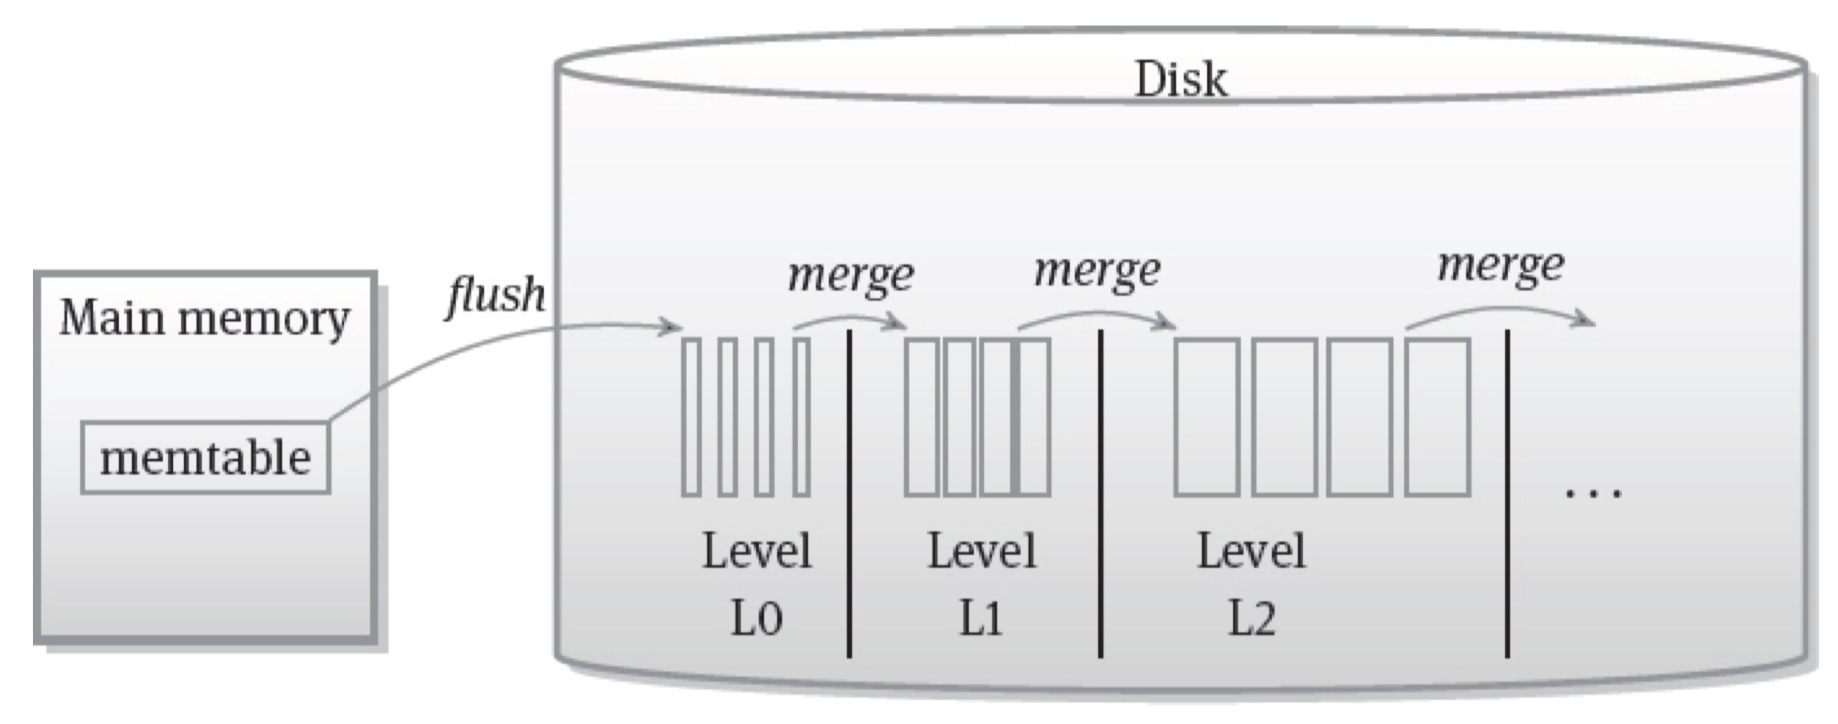
\includegraphics[width=0.70\linewidth]{images/AdvancedDataManagment/extensible_record_store/leveled_compaction.jpeg}
    \caption{Level compaction}
\end{figure}

\subsection{Bloom filters}
A Bloom filter is a probabilistic method to determine set membership for a given value.
\begin{tcolorbox}
For a given value \(c\) and a set \(S\) of values, the \textbf{Bloom filter} is a \textbf{small bit vector} with which we can decide whether \(c\) is \textit{included} in \(S\) without actually searching for \(c\) in \(S\). Of course it comes with a small probability of error.
\end{tcolorbox}

\begin{itemize}
    \item \textbf{True positive:} Bloom filter \textbf{correctly} reports a \textbf{match} and confirms that \(c\) is an element of \(S\). So \(c \in S\) holds
    \item \textbf{False positive:} Bloom filter \textbf{wrongly} reports a \textbf{match}, so it though that\(c \in S\) but actually \(c \notin S\)
    \item \textbf{True negative:} Bloom filter \textbf{correctly} reports a \textbf{miss}, so \(c \notin S\) holds;
    \item \textbf{False negative:} Bloom filter \textbf{erroneously} reports a \textbf{miss}, so it though that\(c \notin S\) but actually \(c \in S\)
\end{itemize}
The only kind of error that could arises are \textbf{False positives}:
\begin{itemize}
    \item When the Bloom filter reports a match we cannot be sure if this is true
    \item We have to actually search for \(c\) in \(S\) to verify whether \(c \in S\) holds
    \item Or whether the Bloom filter wrongly believed \(c\) to be an element of \(S\) although in fact \(c \notin S\) holds
\end{itemize}

For extensible record stores, Bloom filters \textit{can be maintained} for all the row keys in a data file with the following positive effect:
When searching for a given query key in the file, first the Bloom filter is accessed with the query key. If the Bloom filter reports a
\begin{itemize}
    \item \textbf{Miss:} \textit{true negative}, so we do not have to access any data
    \item \textbf{Match:} we have to load the index and search it for the query key to check whether the match was a \textit{true positive} or a \textit{false positive} (which means the record is not found in the data file)
\end{itemize}
Moreover for
\begin{itemize}
    \item \textbf{Small data files:} a single Bloom filter can be appended at the end of the data file
    \item \textbf{Large data file} with lots of keys: a single Bloom filter will be too large. So this will result in performance delays when searching for a row key in the data file.
\end{itemize}
Bloom filter can be broken into pieces, a small Bloom filter “chunk” is maintained for the keys in each block; the Bloom filter chunk is then queried for the existence of a key before actually accessing data in the corresponding block.

\begin{tcolorbox}
A \textbf{Bloom filter} is a bit vector of a chosen length \(m\)
with every position initialized to 0. The bit vector is accompanied by
\(k\) different hash functions \((h_1,...,h_k)\) where each hash function is
assumed to map an arbitrary value \(c\) randomly to a number between
1 and \(m\) – that is, \((h_i(c) \in {1,...,m})\).
\end{tcolorbox}

For each number \(d\) between 1 and \(m\), the probability that an input value \(c\) is mapped to \(d\) should be equal to \(\frac{1}{m}\) this ca be written as \textit{Prob}\((h_i(c) = d) = \frac{1}{m}\)

The case that \textbf{two different input values} \(c\) and \(c'\) are mapped to the same value, so \(h_i(c) = h_i(c')\) we will have a so called \textbf{collision}. Collisions are the reason why false positives can occur with Bloom filter.
\newpage
\begin{figure}[!h]
    \centering
    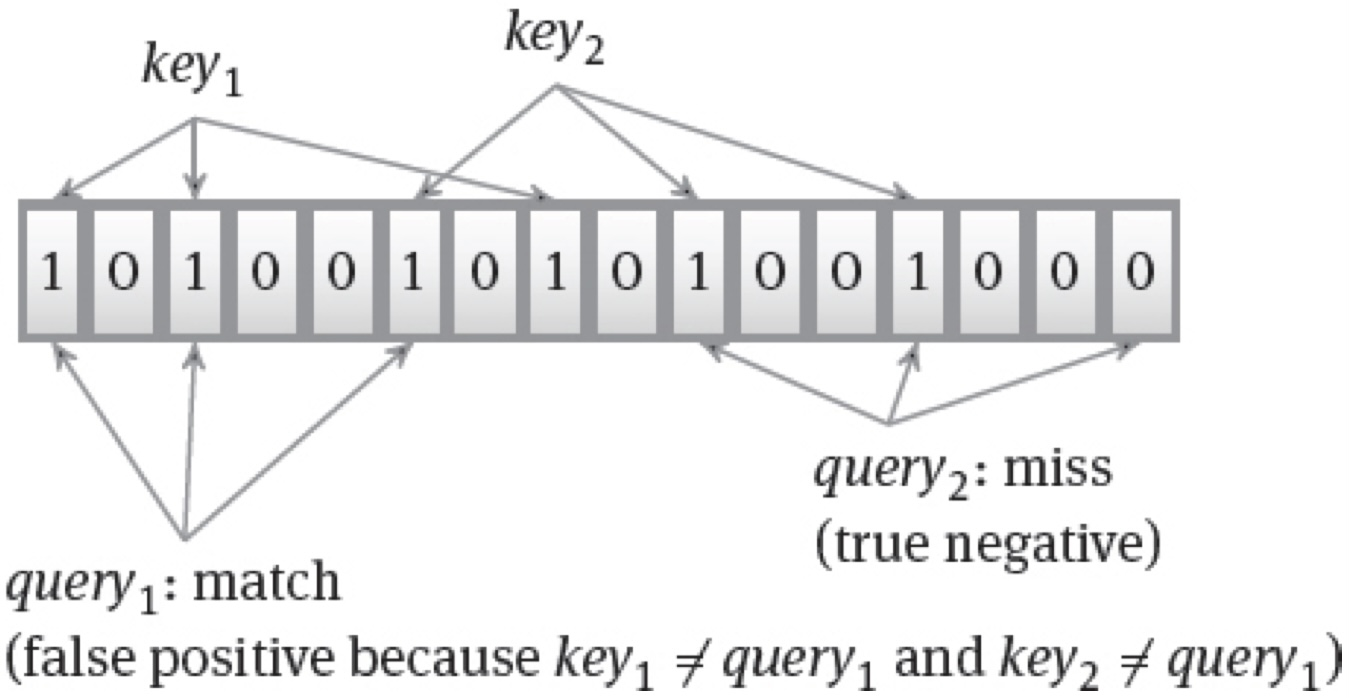
\includegraphics[width=0.50\linewidth]{images/AdvancedDataManagment/extensible_record_store/bloom_filter.jpeg}
    \caption{Bloom filter}
\end{figure}

The rate of false positive is approxiamted as:
\begin{tcolorbox}
\[\biggl(1 - \biggl(1 - \frac{1}{m}\biggl)^{k \cdot n}\biggl)^k \approx (1 - e^{\frac{-k \cdot n}{m}})^k\]
\end{tcolorbox}
With \(k\) as the number of hash functions, \(m\) as the Bloom Filter length and \(n\) as the number of input keys.

\chapter{Graph Databases}
A graph is a structure that not only can represent data but also connections between them; in particular, links between data items are explicitly represented in graphs.

\section{Graphs and Graph Structures}
Graphs structure data into a set of data objects and a set of links between these objects. The \textit{data objects} are the \textbf{nodes} (vertices) and \textit{links} are the \textbf{edges} (arcs).

\begin{tcolorbox}
Graphs can store information in the nodes as well as on the edges.
\end{tcolorbox}

In a social network the \textbf{nodes} of a graph can store \textit{information on people} and \textbf{edges} can store their \textit{acquaintance} or express \textit{sympathy} or \textit{antipathy}.

Or in a geographic information systems \textbf{nodes} store information on \textit{geographical locations} like cities and \textbf{edges} store for example the \textit{distances} between the locations

\begin{figure}
     \centering
     \begin{subfigure}[b]{0.45\textwidth}
         \centering
         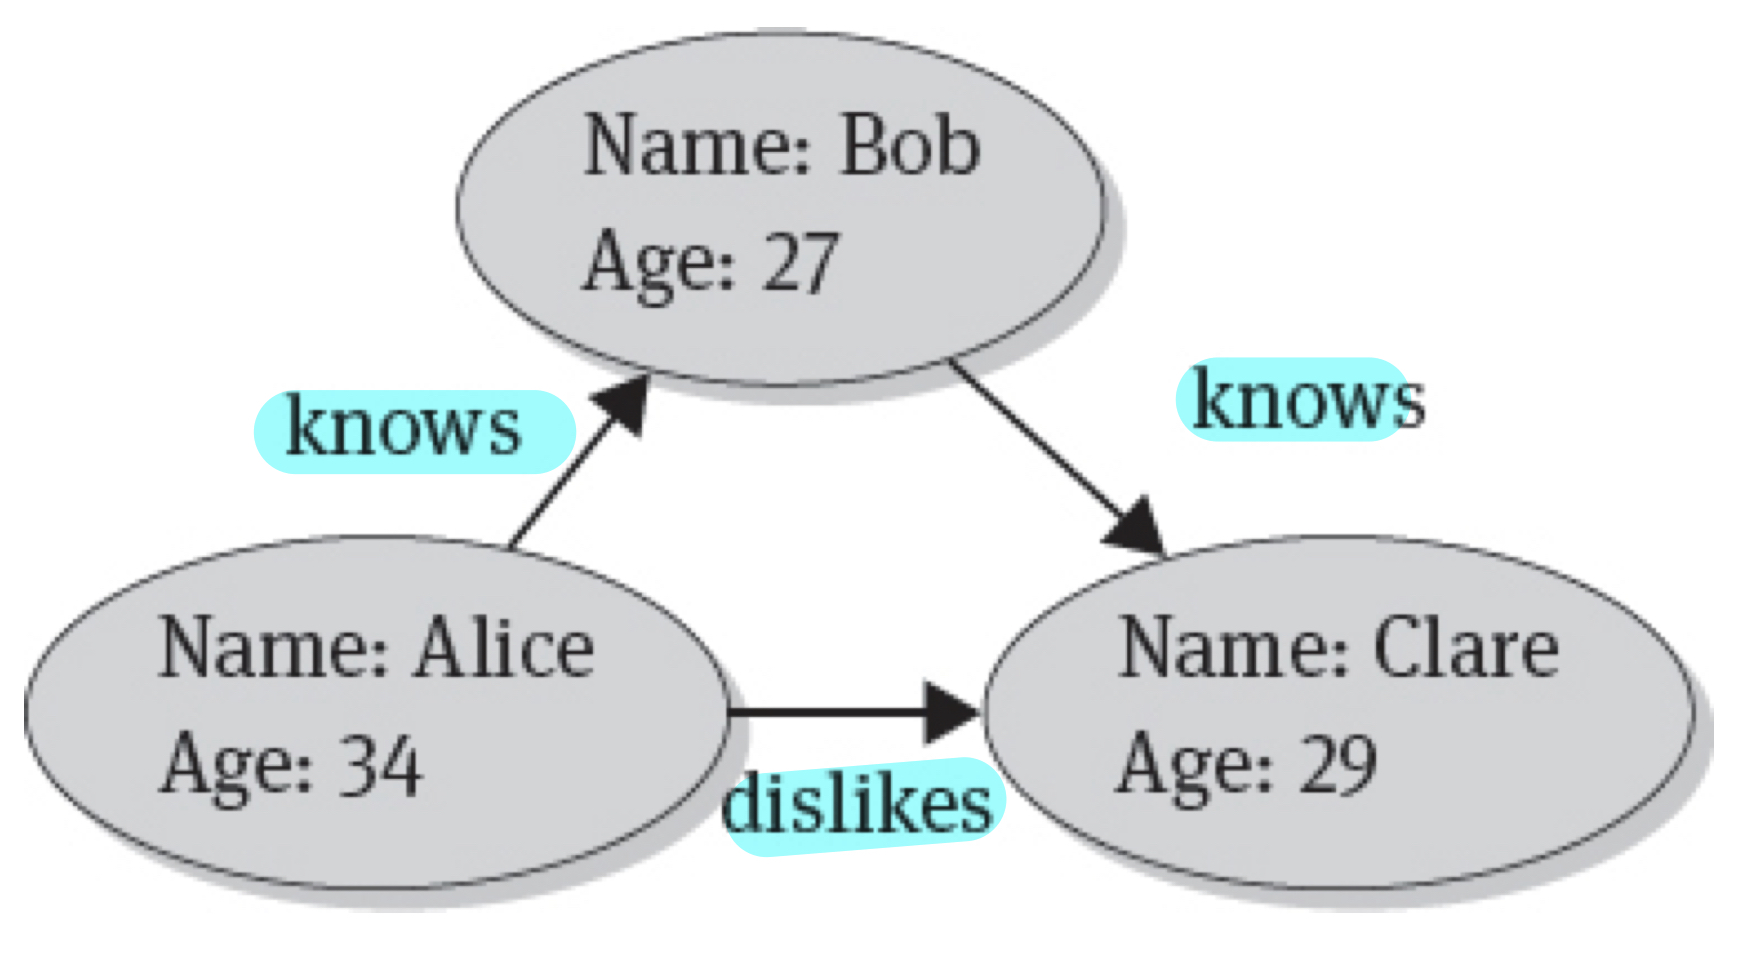
\includegraphics[width=\textwidth]{images/AdvancedDataManagment/graph_databases/social_network_example.jpeg}
         \caption{A social network as a graph}
     \end{subfigure}
     \hfill
     \begin{subfigure}[b]{0.45\textwidth}
         \centering
         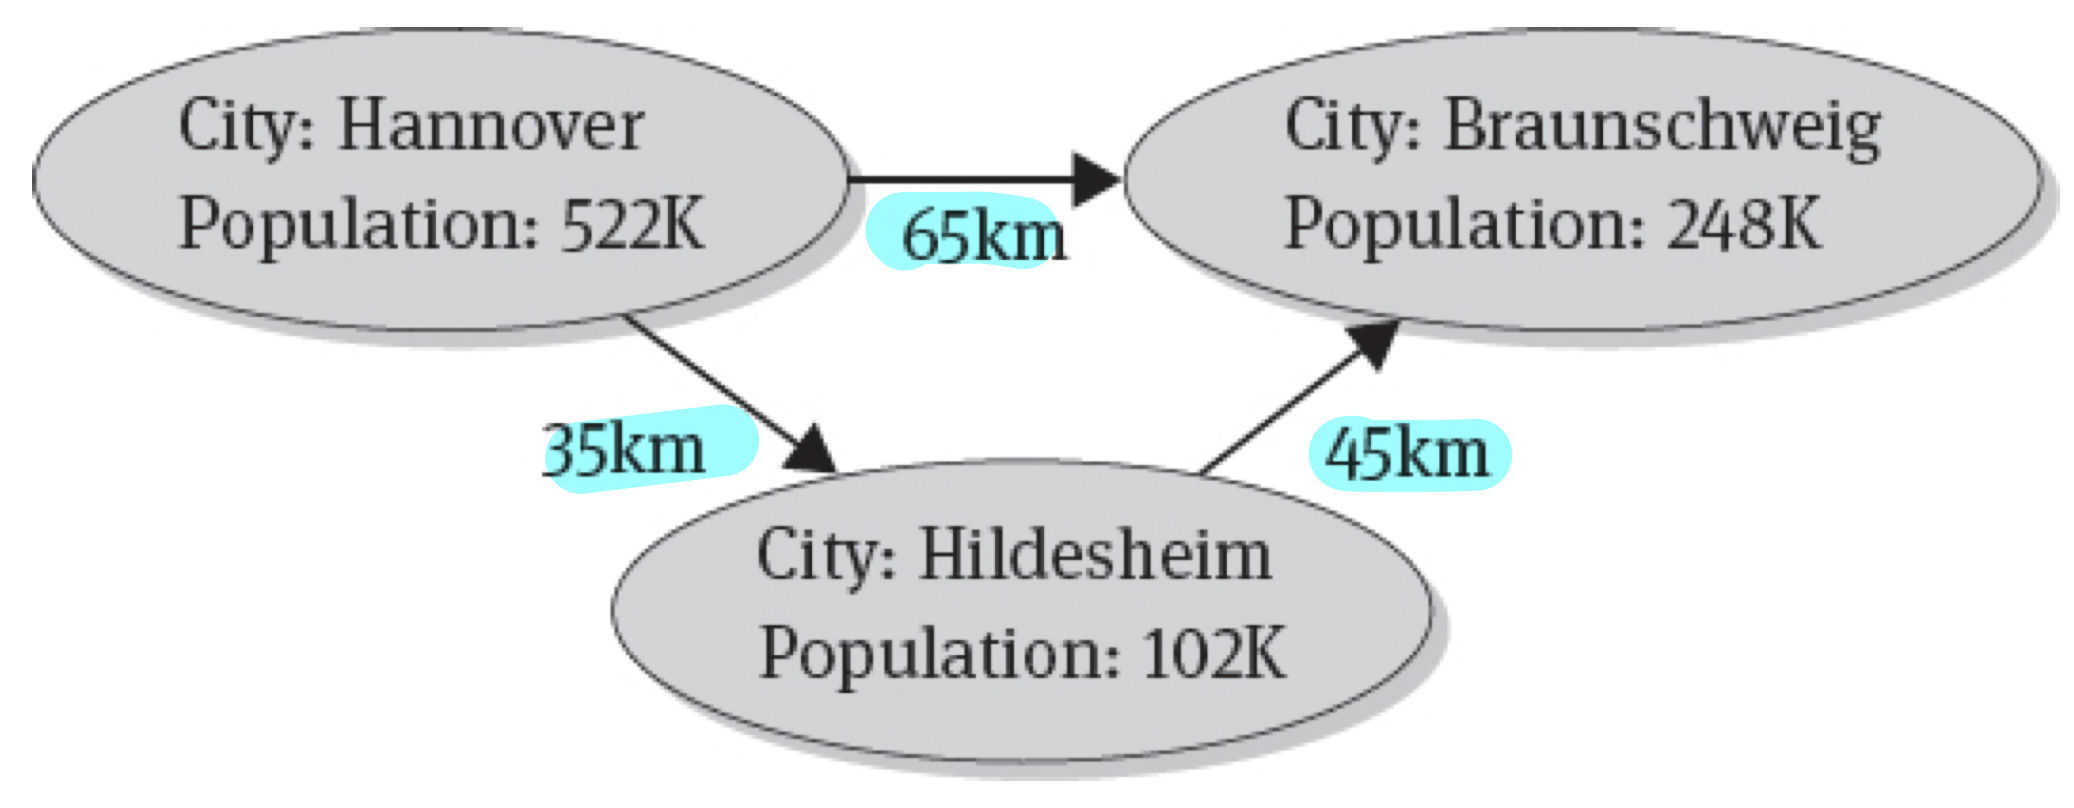
\includegraphics[width=\textwidth]{images/AdvancedDataManagment/graph_databases/geographical_example.jpeg}
         \caption{Geographical data as a graph}
     \end{subfigure}
\end{figure}

\subsection{A Glimpse on Graph Theory}
Mathematically speaking a graph \(G = (V, E)\) consists on a set of nodes \(V\) and a set of edges \(E\).
\begin{itemize}
    \item The edge set \(E\) is a set of pairs of nodes and represents vertices that are connected by the edge
    \item The edge can be \textit{directed} or \textit{undirected}:
    \begin{itemize}
        \item In a \textit{directed} edge the pair of nodes is ordered where the first node is the \textbf{source} node of the edge and the last node is the \textbf{target} node
        \item In the \textit{undirected} case, order of the pair of nodes does not matter 
    \end{itemize}
\end{itemize}
Moreover, a graph is called \textit{multigraph} if it has a pair of nodes that is connected by more than one edge. Now we have a look on a short summary on the graph types:

\begin{itemize}
    \item \textbf{Simple undirected graph:}
    \begin{figure}[!h]
        \centering
        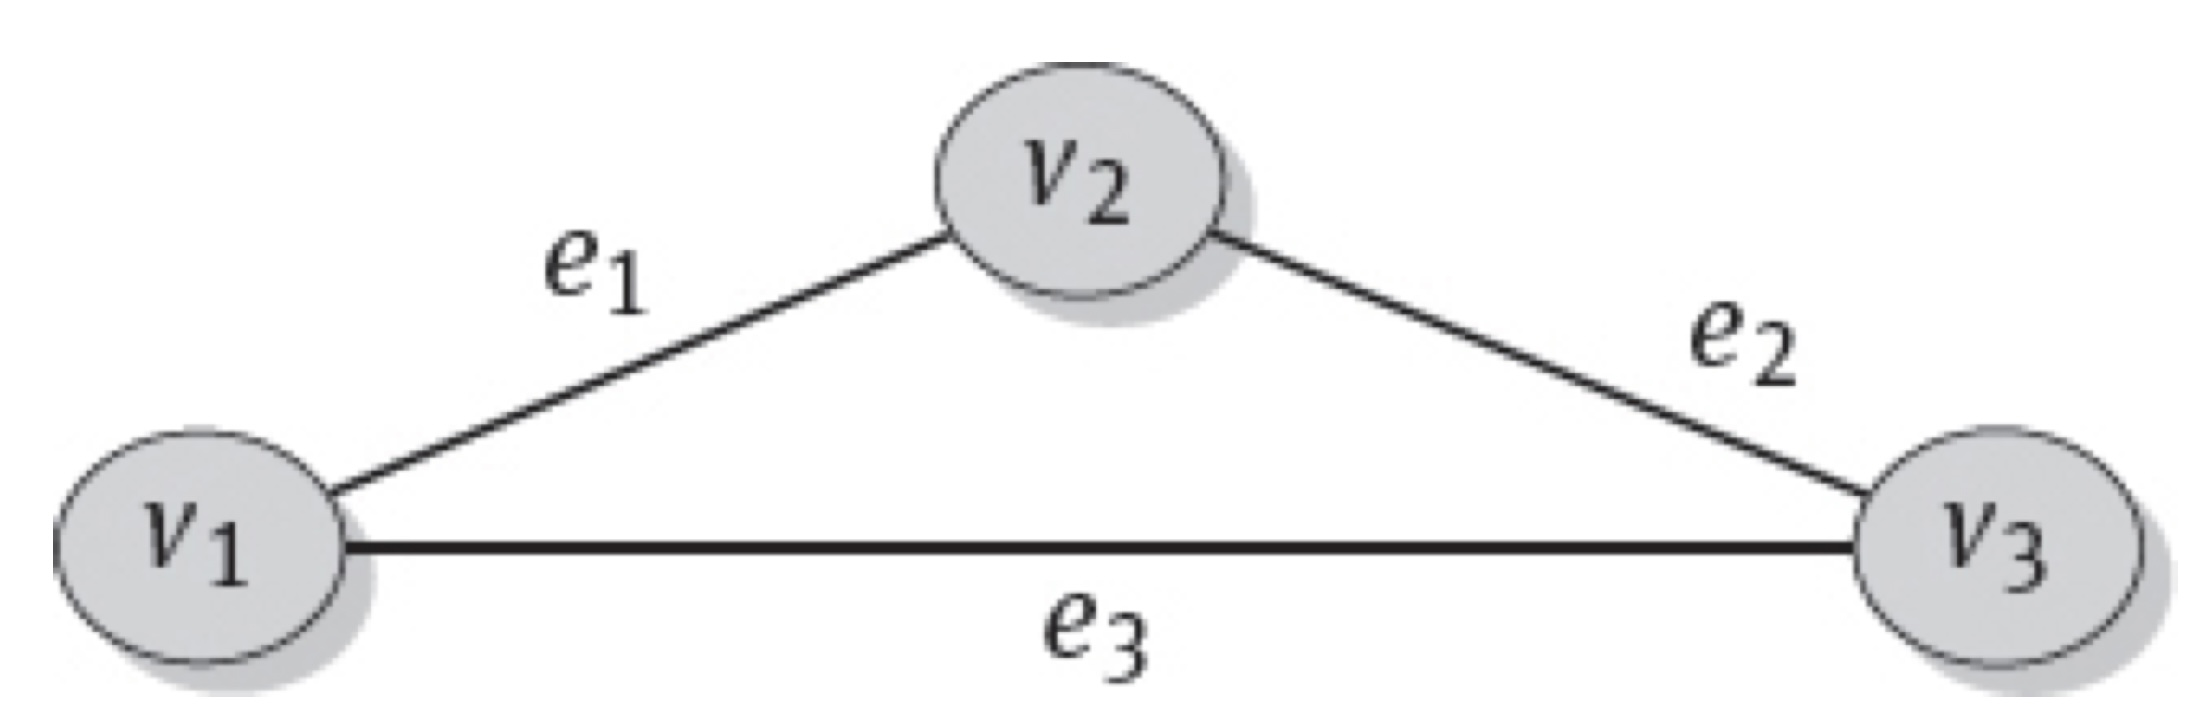
\includegraphics[width=0.35\linewidth]{images/AdvancedDataManagment/graph_databases/simple_undirected_graph.jpeg}
    \end{figure}
    
    \item \textbf{Simple directed graph:}
    \begin{figure}[!h]
        \centering
        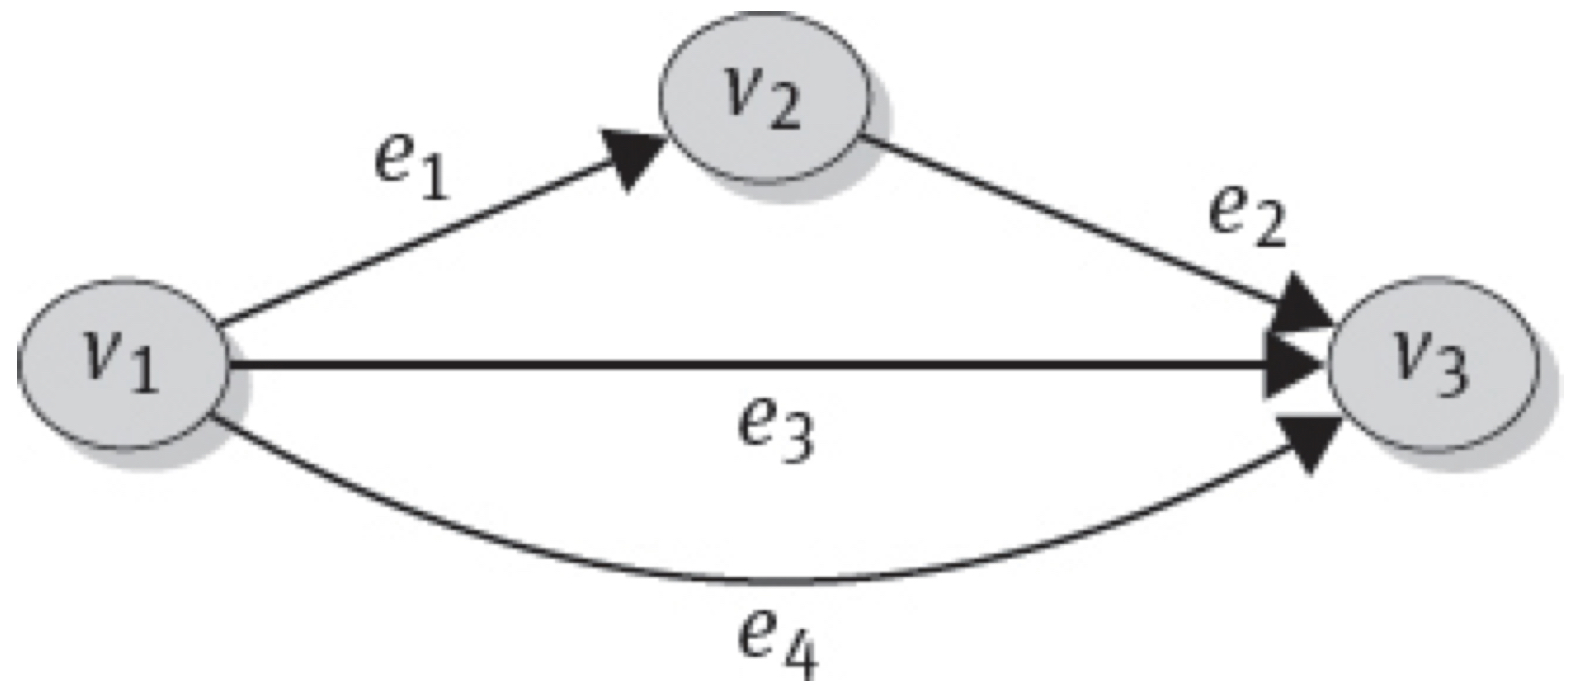
\includegraphics[width=0.35\linewidth]{images/AdvancedDataManagment/graph_databases/directed_multigraph.jpeg}
    \end{figure}
    
    \item \textbf{Undirected Multigraph:}
    \begin{figure}[!h]
        \centering
        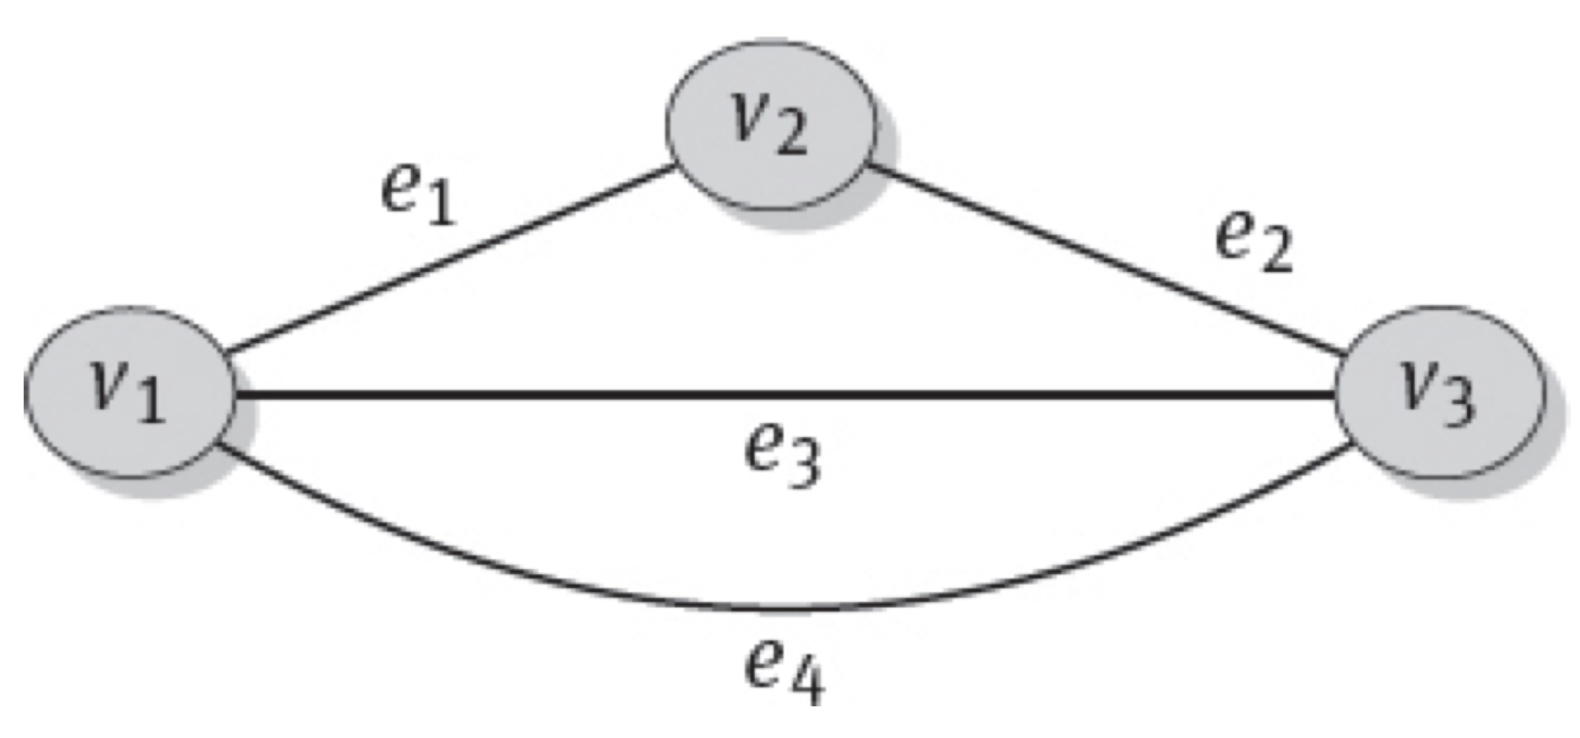
\includegraphics[width=0.35\linewidth]{images/AdvancedDataManagment/graph_databases/undirected_multigraph.jpeg}
    \end{figure}
    
    \item \textbf{Directed Multigraph:}
    \begin{figure}[!h]
        \centering
        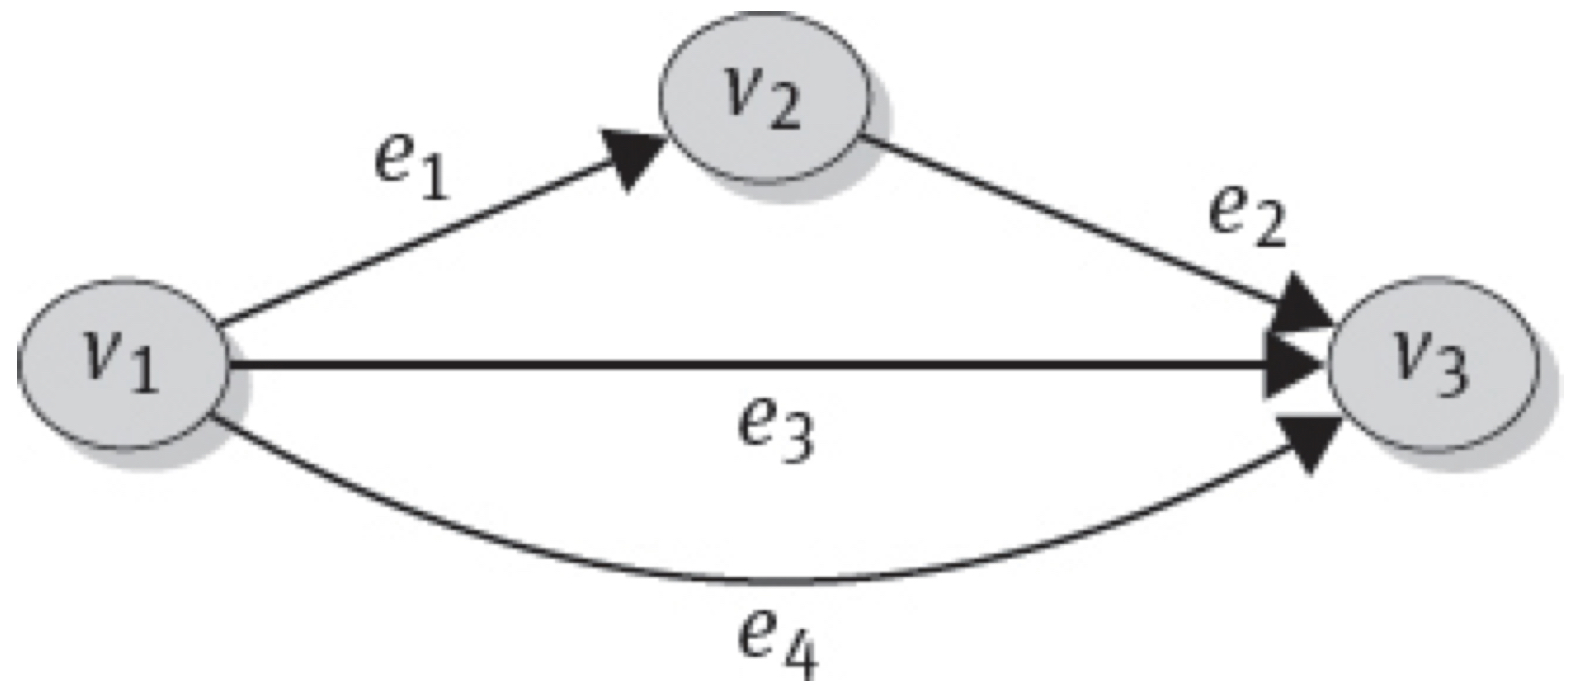
\includegraphics[width=0.35\linewidth]{images/AdvancedDataManagment/graph_databases/directed_multigraph.jpeg}
    \end{figure}
    
    \item \textbf{Weighted graphs:}
    \begin{figure}[!h]
        \centering
        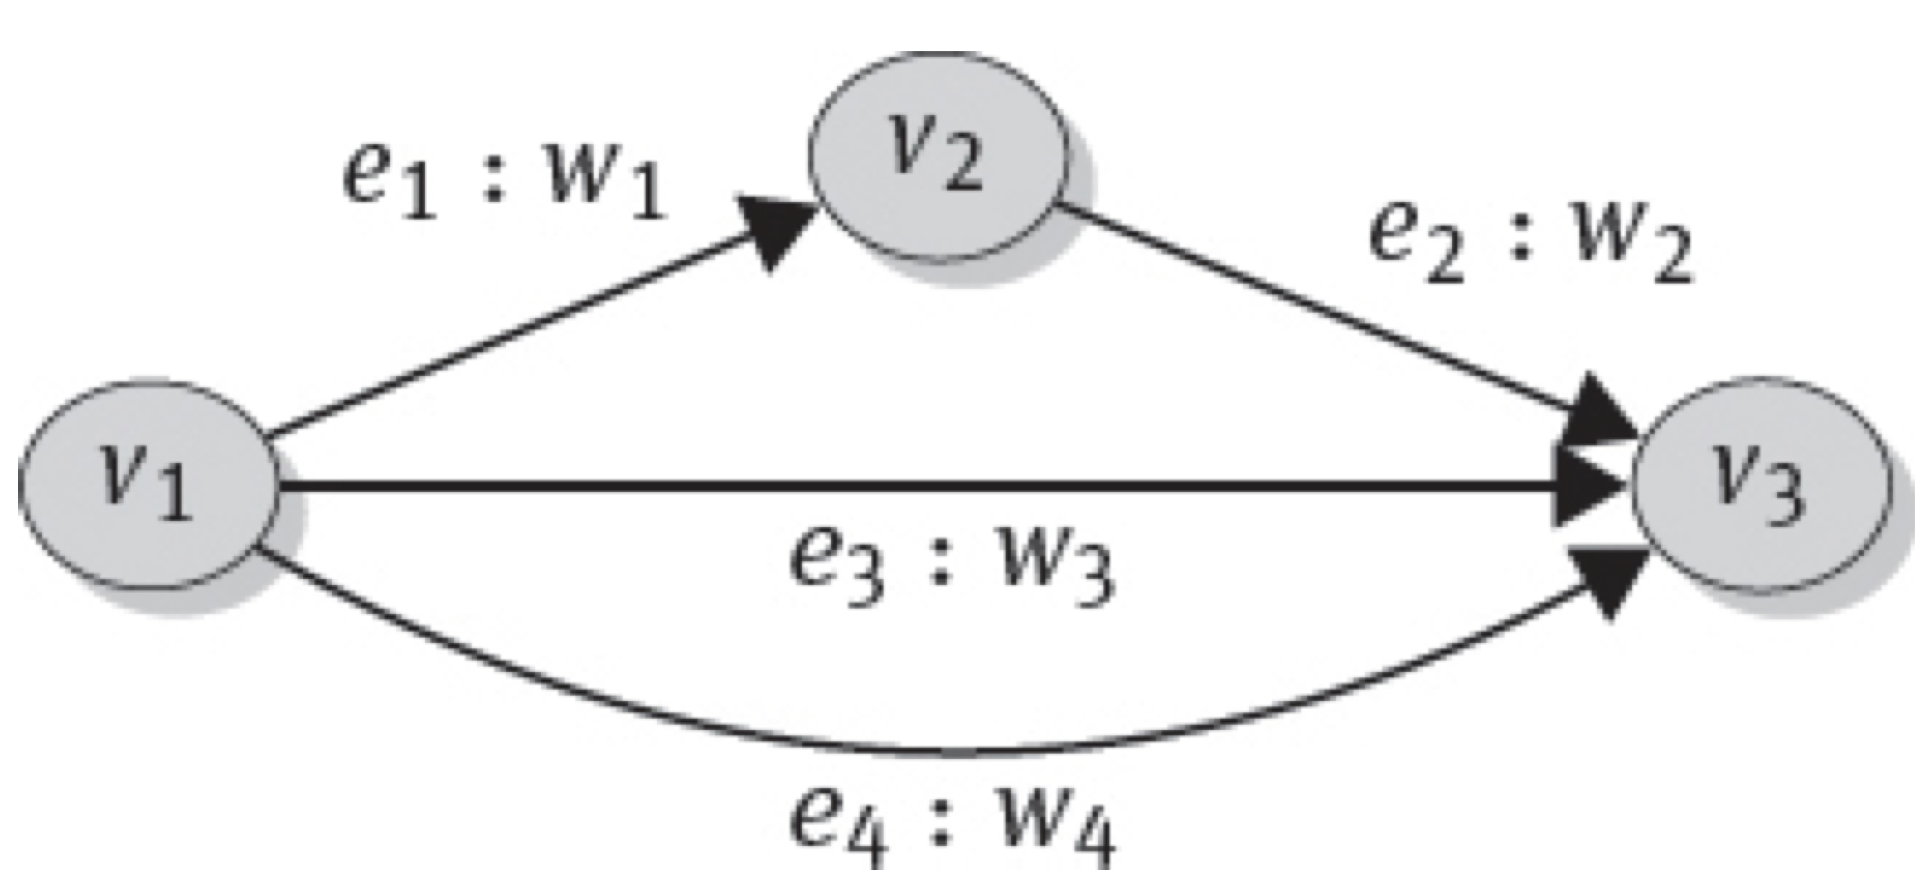
\includegraphics[width=0.35\linewidth]{images/AdvancedDataManagment/graph_databases/weighted_graph.jpeg}
    \end{figure}
\end{itemize}

\subsection{Graph Traversal and Graph Problems}
\begin{itemize}
    \item A connection between to nodes consisting of intermediary nodes and the edges between them is called a \textbf{path}
    \item A path where starting node and end node are the same is called a \textbf{cycle}
    \item A \textbf{traversal} is a sort of navigation from a starting node to a specific destination nodes towards adjacent nodes. It could be:
    \begin{itemize}
        \item \textit{full} visiting each and every node in a graph
        \item \textit{partial} in which navigation may be restricted by a certain depth of paths to be followed
    \end{itemize}
\end{itemize}
When traversing a graph, restrictions may be applied that have come to known as \textbf{graph problems}:
\begin{itemize}
    \item \textbf{Eulerian Path:} a path that visits each edge exactly once;
    \item \textbf{Eulerian Cycle:} a cycle that visits each edge exactly once;
    \item \textbf{Hamiltonian Path:} a path that visits each vertex exactly once
    \item \textbf{Hamiltonian Cycle:} a cycle that visits each vertex exactly once
    \item \textbf{Spanning Tree:} a subset of the edge set V that forms a tree and visits each node of the tree
\end{itemize}

\section{Graph Data Structures}
When computing with graphs, the information on nodes and their connecting edges has to be represented and stored in an appropriate data structure. Two important terms in this field are \textbf{adjacency} and \textbf{incidence}
\begin{tcolorbox}
Two nodes are \textbf{adjacent} if they are neighbors (that is, there is an edge between them)
\end{tcolorbox}

\begin{tcolorbox}
An edge is \textbf{incident} to a node, if it is connected to the node. Moreover if the edge is \textit{directed}:
\begin{itemize}
    \item It is \textbf{positively incident} to its \textit{source} node
    \item And \textbf{negatively incident} to its \textit{target} node
\end{itemize}
A node is incident to an edge, if it is connected to the edge.
\end{tcolorbox}

\subsection{Edge List}
The graph can be stored according to the mathematical definition as a set of nodes \(V\) and a set (or list) of edges \(E\). Edges could be represented as:
\begin{itemize}
    \item \textit{A set of sets} for \textbf{undirected graphs}
    \item \textit{A multiset set} for \textbf{multigraphs}
\end{itemize}
We can compute the classical operation:
\begin{itemize}
    \item \textbf{Addition} of an edge or nodes in which we simply add the element in the respective set
    \item \textbf{Deletion} by simply deleting the removed node or edge from the respective set
    \item \textbf{Search} the edge set performs well when one wants to retrieve all edges of the graph at once
\end{itemize}
However, the edge list representation is ineffcient in most use cases, like: looking for one particular edge or getting all neighbors of a given node requires \textit{iterating over the entire edge list}

\subsection{Adjacency Matrix}
\begin{itemize}
    \item For cardinality \(|V| = n\) the adjacent matrix is \(n \times n\) matrix
    \item Rows and columns denoted by \(v_1,...,v_n\)
    \item \textbf{Simple undirected graphs}
    \begin{itemize}
        \item If between \(v_i\) and \(v_j\) there is an edge we put a \(1\) in the corresponding cells \((v_i, v_j)\) and \((v_j, v_i)\) since \textit{symmetry}
        \item In case of \textit{loops} \(v_i, v_i\) we write \(2\) in the diagonal cell  \(v_i, v_i\)
        
        \begin{figure}[!h]
        \centering
        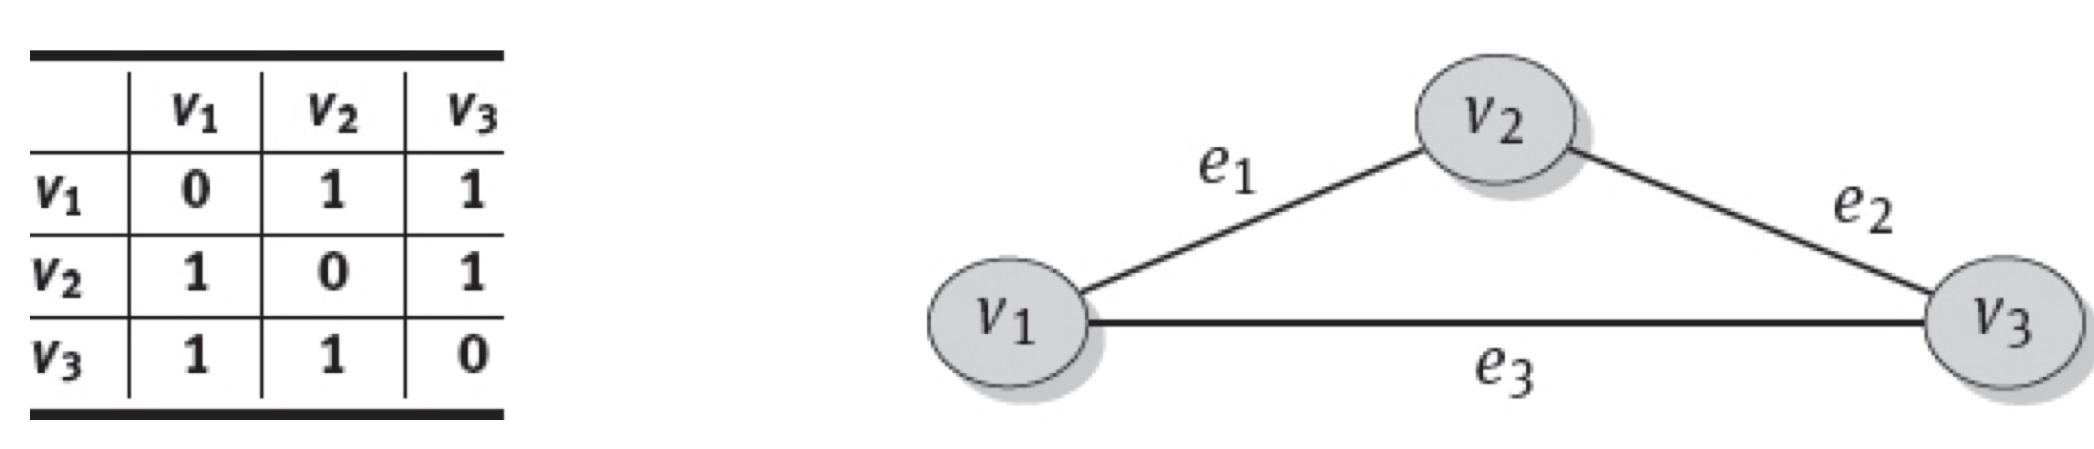
\includegraphics[width=0.7\linewidth]{images/AdvancedDataManagment/graph_databases/adj_matrix_simple_undirected.jpeg}
        \end{figure}
        
    \end{itemize}
    \item \textbf{Simple directed graph}
    \begin{itemize}
        \item If between \(v_i\) and \(v_j\) there is an edge we put a \(1\) in the corresponding cell \((v_i, v_j)\) since \textit{asymmetry}
        \item In case of \textit{loops} \(v_i, v_i\) we write \(1\) in the diagonal cell \(v_i, v_i\)
    
        \begin{figure}[!h]
        \centering
        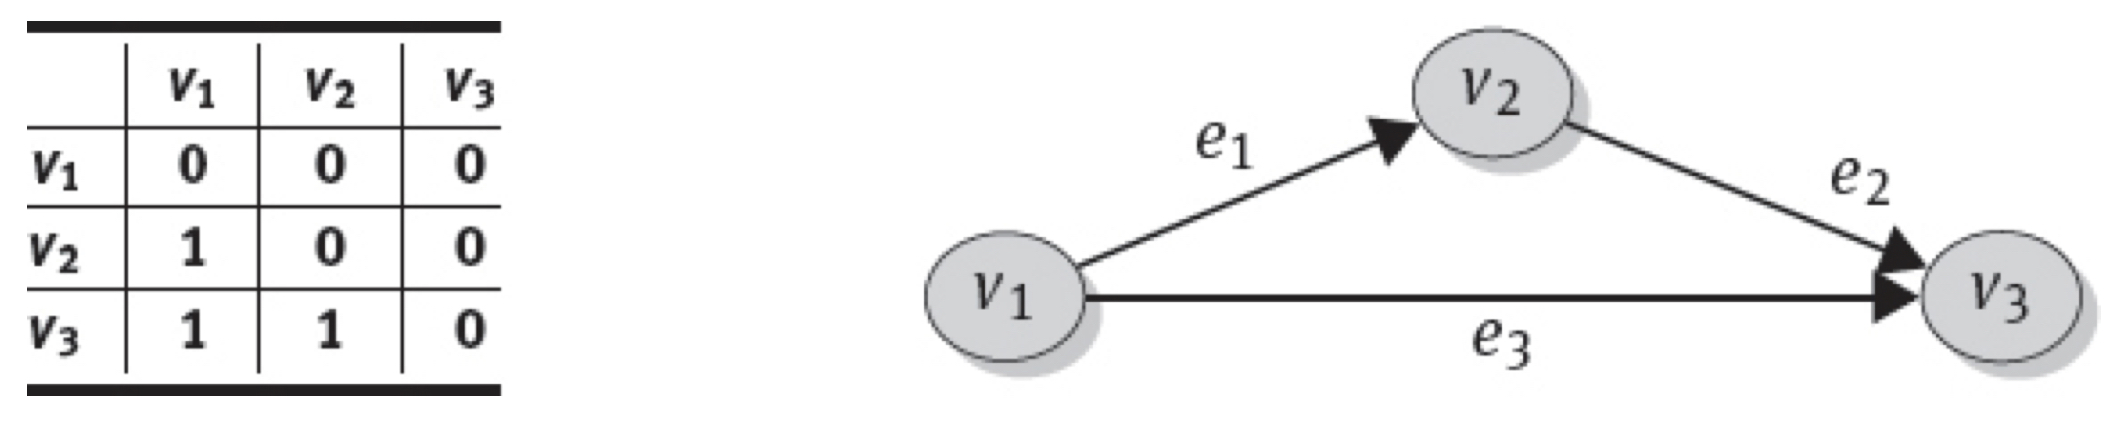
\includegraphics[width=0.7\linewidth]{images/AdvancedDataManagment/graph_databases/adj_matrix_simple_directed.jpeg}
        \end{figure}
        
    \end{itemize}
    \item \textbf{Undirected multigraph}
    \begin{itemize}
        \item If there are \(k\) edges between \(v_i\) and \(v_j\) we put a \(k\) in the corresponding cells \((v_i, v_j)\) and \((v_j, v_i)\) since \textit{symmetry}
        \item In case of \(k\) \textit{loops} \(v_i, v_i\) we write \(2 \cdot k\) in the diagonal cell \(v_i, v_i\)
    
        \begin{figure}[!h]
        \centering
        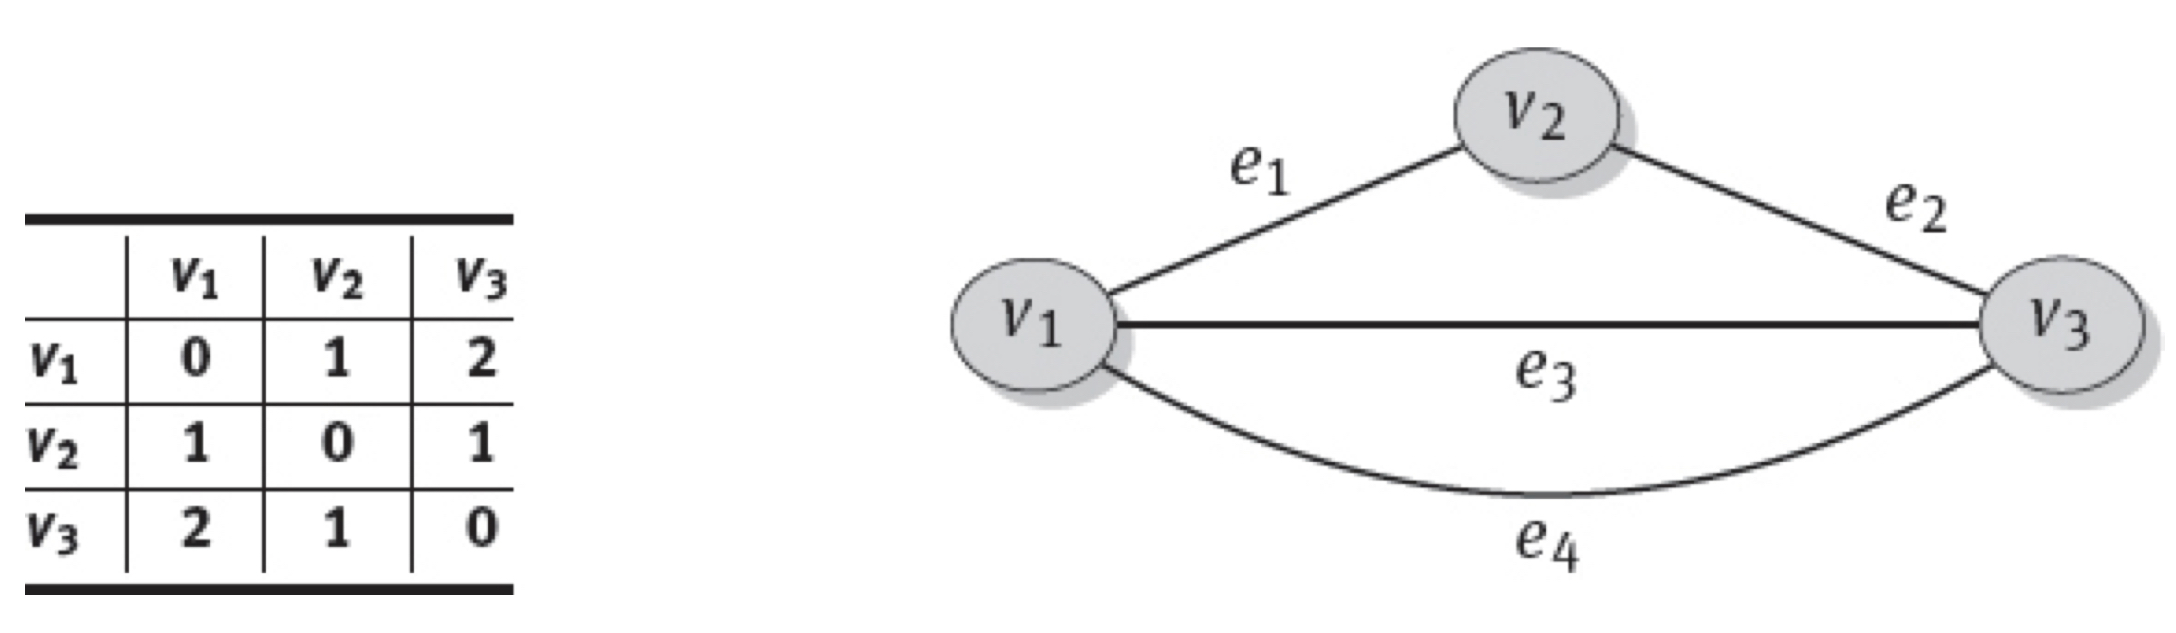
\includegraphics[width=0.7\linewidth]{images/AdvancedDataManagment/graph_databases/adj_matrix_multi_undirected.jpeg}
        \end{figure}
        
    \end{itemize}
    \item \textbf{Directed multigraph}
    \begin{itemize}
        \item If there are \(k\) edges between \(v_i\) and \(v_j\) we put a \(k\) in the corresponding cell \((v_i, v_j)\) since \textit{asymmetry}
        \item In case of \(k\) \textit{loops} \(v_i, v_i\) we write \(k\) in the diagonal cell \(v_i, v_i\)
    
        \begin{figure}[!h]
        \centering
        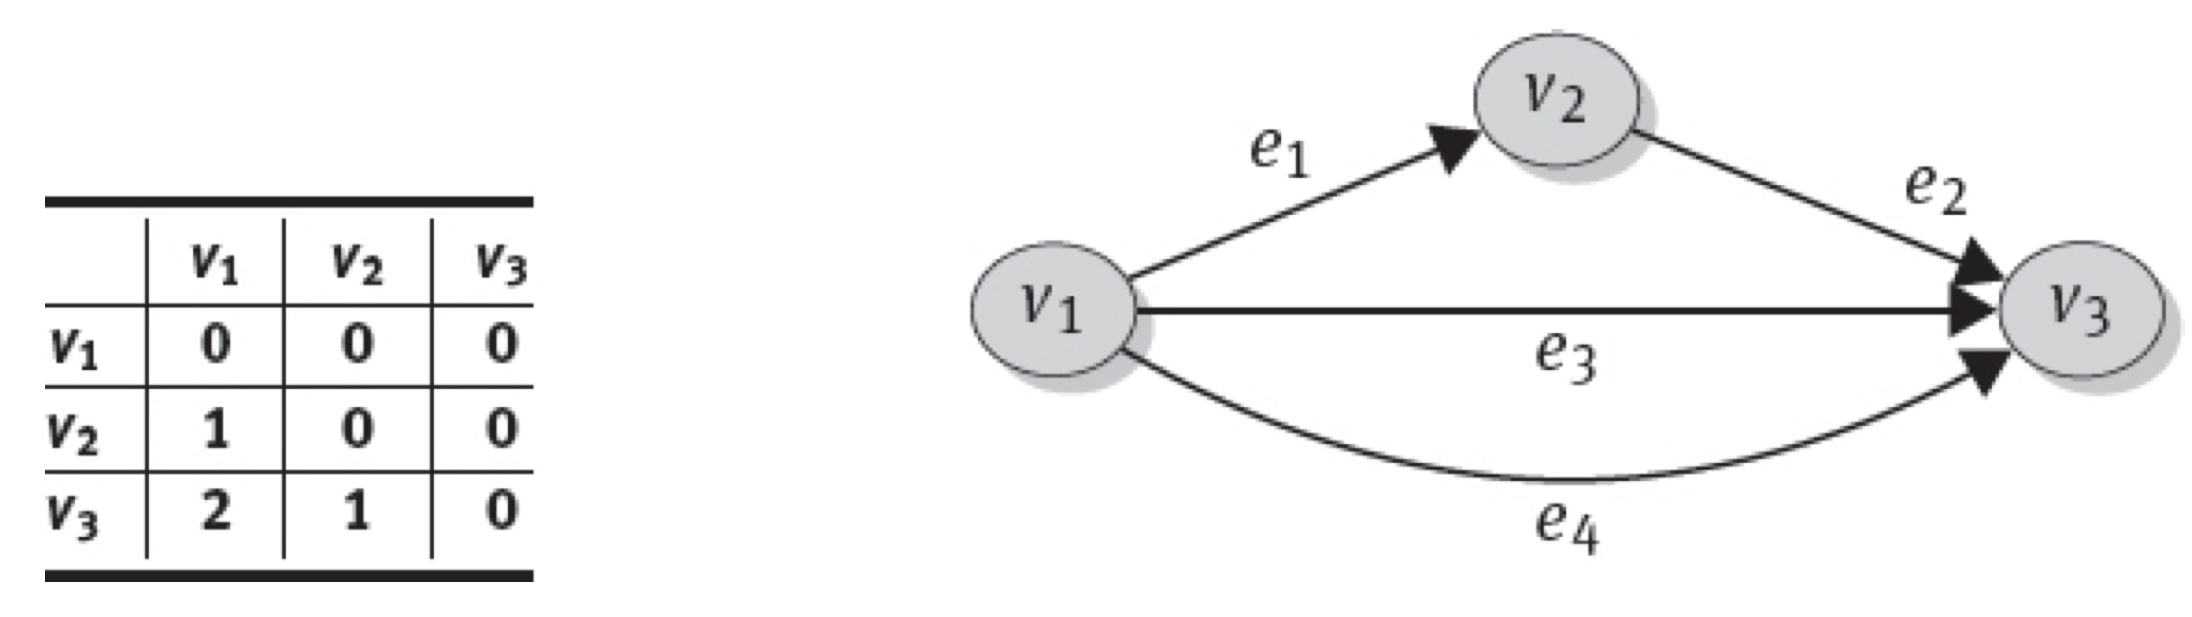
\includegraphics[width=0.7\linewidth]{images/AdvancedDataManagment/graph_databases/adj_matrix_multi_directed.jpeg}
        \end{figure}
        
    \end{itemize}
\end{itemize}
\subsubsection{Advantages}
\begin{itemize}
    \item Quick lookup of existence of a single edge by looking at the bit value of the matrix
    \item Quick insertion of new edge by incrementing the bit in the matrix cell
\end{itemize}

\subsubsection{Disadvantages}
\begin{itemize}
    \item Adding a new node requires insertion of a new row and a new column and finding all neighbors results in a scan of the entire column
    \item \(n \times n\) matrices are heavy
    \item Unnecessary information, indeed lots of 0s in the rows
    \item No hyperedges can be stored (edges that connects a set of nodes)
\end{itemize}

\subsection{Incidence Matrix}
\begin{itemize}
    \item For cardinality \(|V| = n\) and \(|E| = m\) the incidence matrix is \(n \times m\) matrix
    \item Rows denote vertices \(v_1,...,v_n\) and columns denote edges \(e_1,...,e_m\)
    \item \textbf{Simple undirected graph}
    \begin{itemize}
        \item If vertices \(v_i\) is connected to edge \(e_j\) we write \(1\) in the corresponding cell \((v_i, e_j)\)
        \item In case of \textit{loop} \(e_j = \{v_i, v_i\}\) we write \(2\) in the corresponding cell \((v_i, e_j)\)
    \end{itemize}
    
    \begin{figure}[!h]
        \centering
        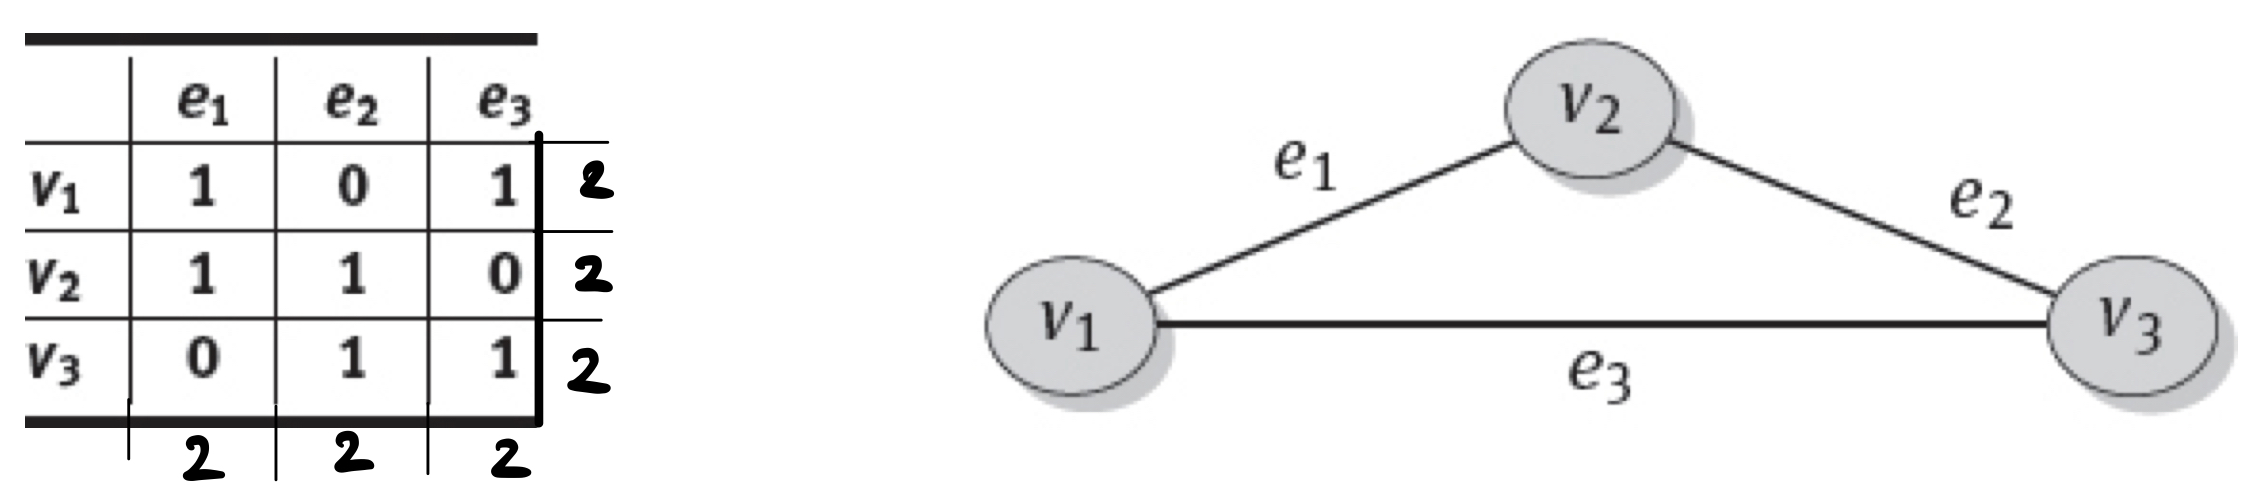
\includegraphics[width=0.7\linewidth]{images/AdvancedDataManagment/graph_databases/inc_matrix_simple_undirected.jpeg}
        \end{figure}
    
    \item \textbf{Simple directed graph}
    \begin{itemize}
        \item For edge \(e_k = (v_i, v_j)\) we write \(-1\) in cell \((v_i, e_k)\) and \(1\) in cell \((v_j, e_k)\)
        \item In case of \textit{loop} \(e_k = \{v_i, v_i\}\) we write \(2\) in the corresponding cell \((v_i, e_k)\)
    \end{itemize}
    
    \begin{figure}[!h]
        \centering
        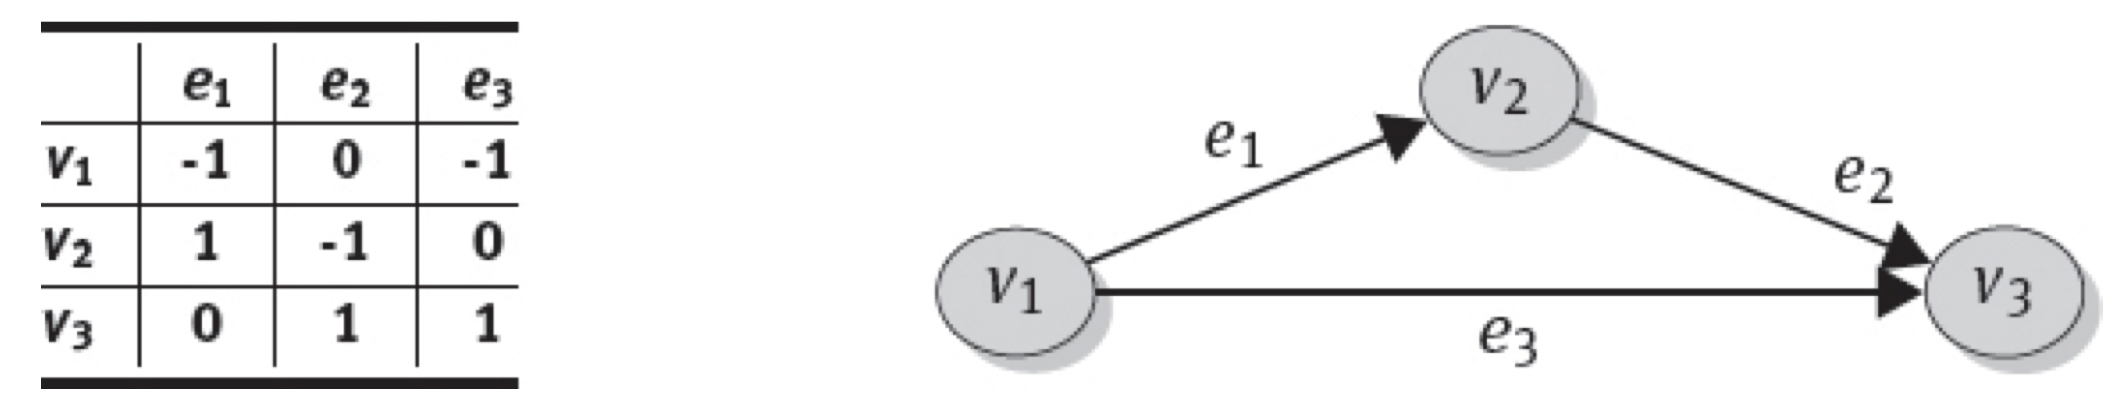
\includegraphics[width=0.7\linewidth]{images/AdvancedDataManagment/graph_databases/inc_matrix_simple_directed.jpeg}
        \end{figure}
    
    \item \textbf{Undirected multigraph}
    \begin{itemize}
        \item If vertices \(v_i\) is connected to edge \(e_j\) we write \(1\) in the corresponding cell \((v_i, e_j)\)
        \item In case of \textit{loop} \(e_j = \{v_i, v_i\}\) we write \(2\) in the corresponding cell \((v_i, e_j)\)
    \end{itemize}
    
    \begin{figure}[!h]
        \centering
        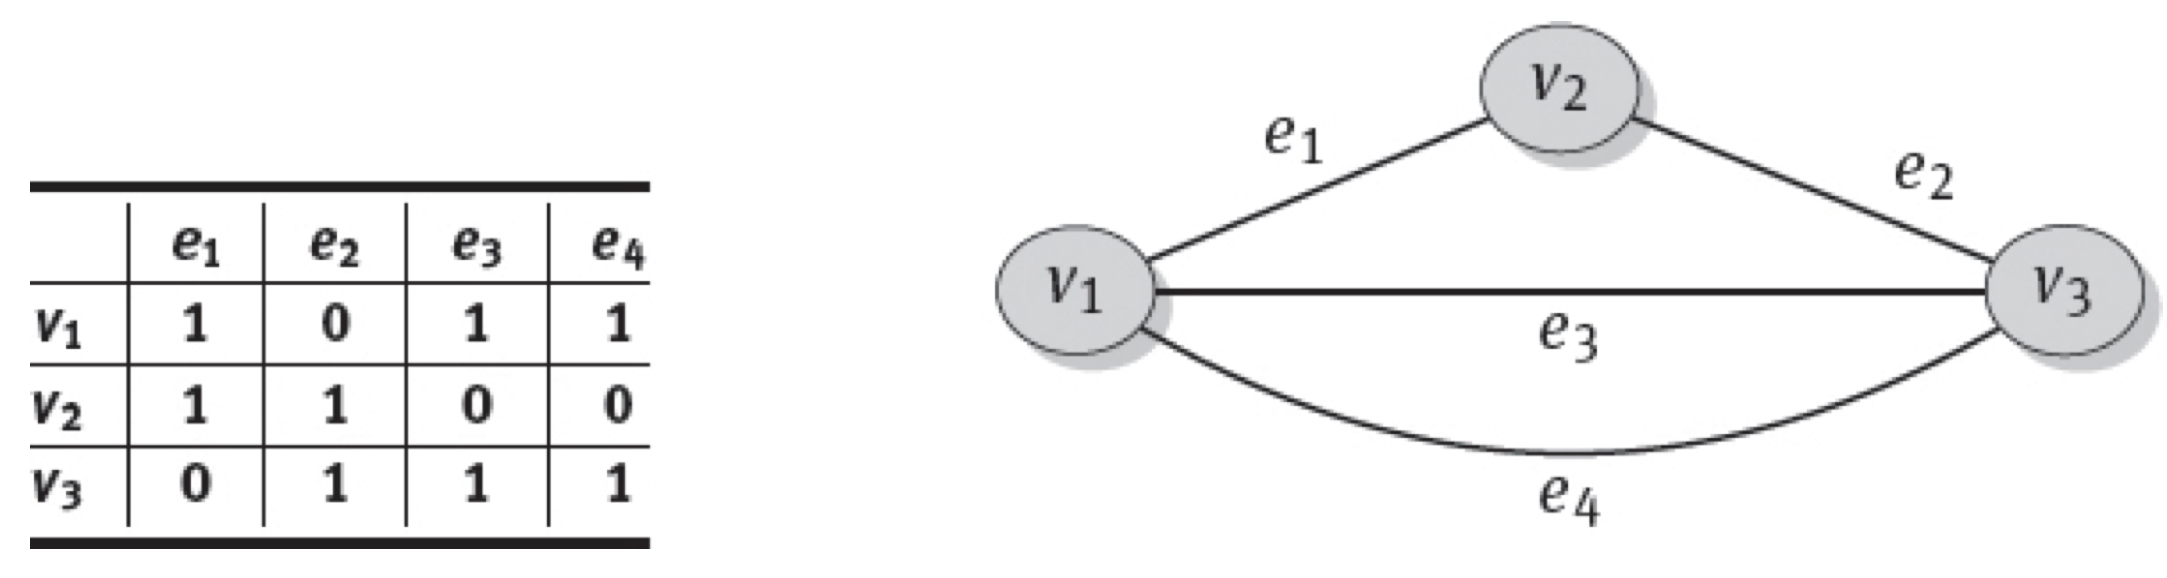
\includegraphics[width=0.7\linewidth]{images/AdvancedDataManagment/graph_databases/inc_matrix_multi_undirected.jpeg}
        \end{figure}
    \newpage
    \item \textbf{Directed multigraph}
    \begin{itemize}
        \item For edge \(e_k = (v_i, v_j)\) we write \(-1\) in cell \((v_i, e_k)\) and \(1\) in cell \((v_j, e_k)\)
        \item In case of \textit{loop} \(e_k = \{v_i, v_i\}\) we write \(2\) in the corresponding cell \((v_i, e_k)\)
    \end{itemize}
    
    \begin{figure}[!h]
        \centering
        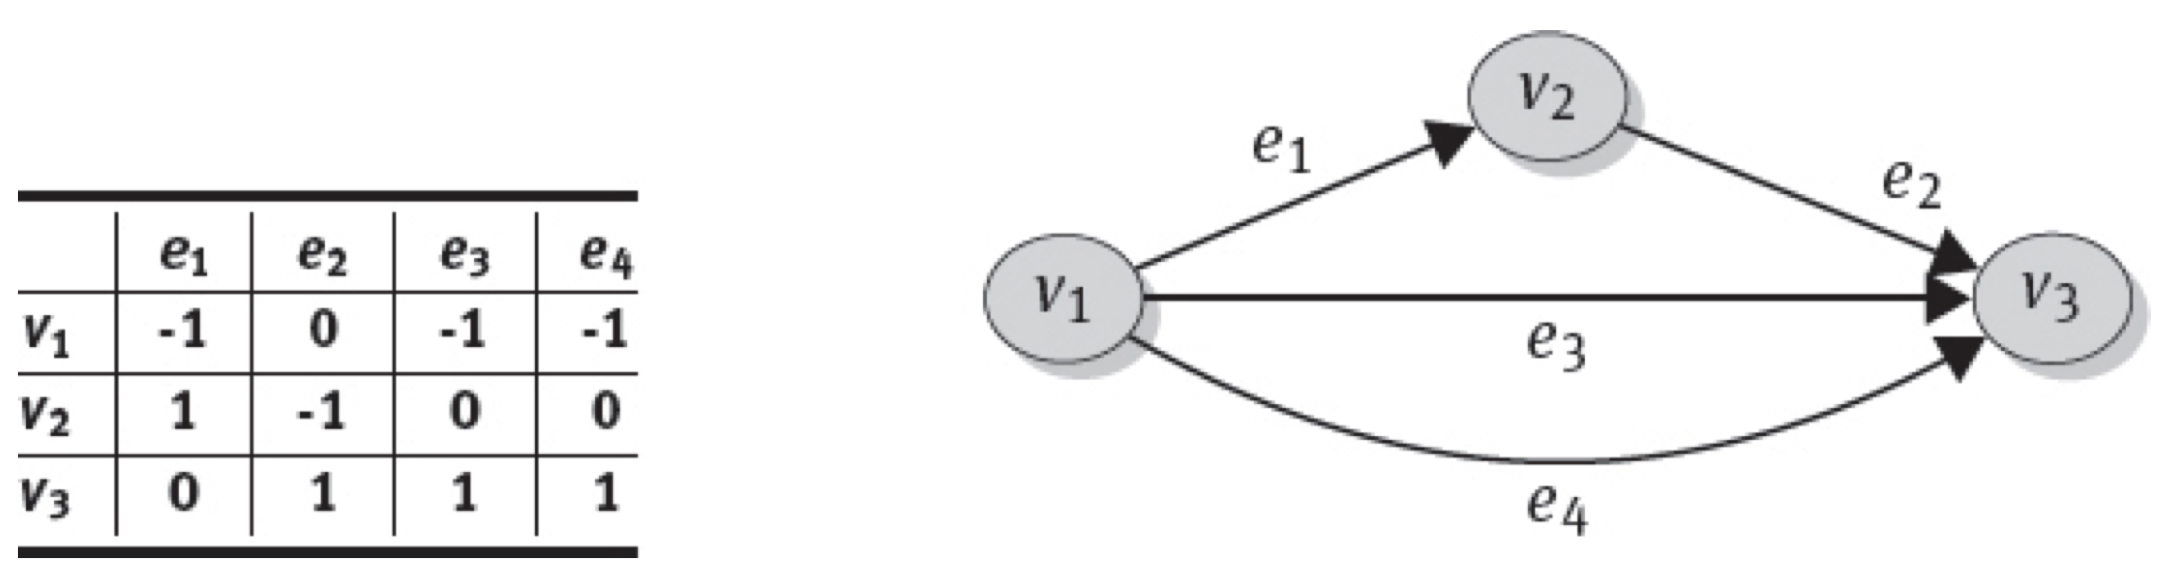
\includegraphics[width=0.7\linewidth]{images/AdvancedDataManagment/graph_databases/inc_matrix_multi_directed.jpeg}
        \end{figure}
    
    
\end{itemize}
\subsubsection{Advantages}
\begin{itemize}
    \item Only existing edges are stored, there is no column with only 0 entries
    \item Hyperedges can be stored
\end{itemize}

\subsubsection{Disadvantages}
\begin{itemize}
    \item Insertions of new vertices and edges are costly, since the addition of a row or a column
    \item Determining all neighbors for one vertex requires scanning the entire row and for each non-zero entry
    \item \(n \times n\) matrices are heavy
    \item Unnecessary information, indeed lots of 0s in the columns 
\end{itemize}

Note that \textbf{checking the existence of an edge} is more involved for the \textit{incidence matrix} than for the adjacency matrix: we have to check whether there is a column with appropriate non-zero entries for the source node’s row and the target node’s row.

\subsection{Adjacent List}
It stores the vertex set \(V\) and for each vertex one stores a \textbf{linked list of neighboring}
\begin{itemize}
    \item \textbf{Simple undirected graph:} each edge is stored in the adjacency list of both its vertices
    \begin{figure}[!h]
        \centering
        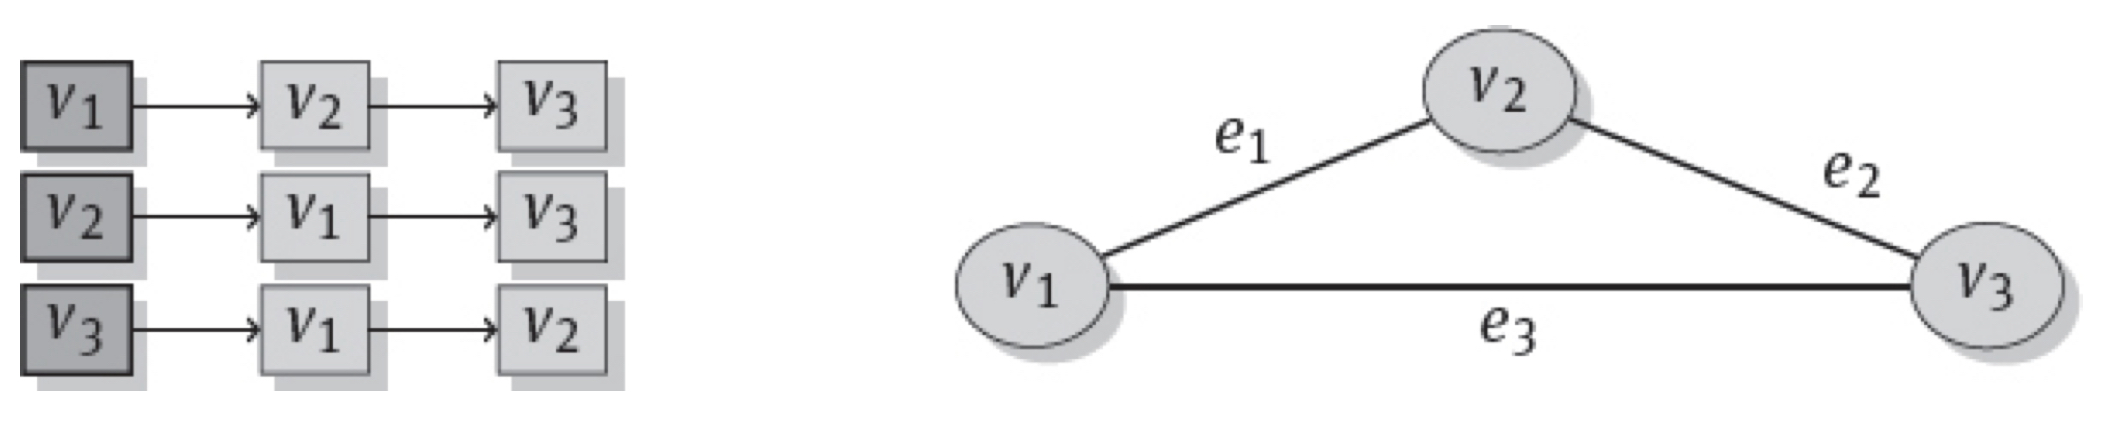
\includegraphics[width=0.7\linewidth]{images/AdvancedDataManagment/graph_databases/adj_list_simple_undirected.jpeg}
        \end{figure}
    \newpage
    \item \textbf{Simple directed graph:} it stores only outgoing edges
    \begin{figure}[!h]
        \centering
        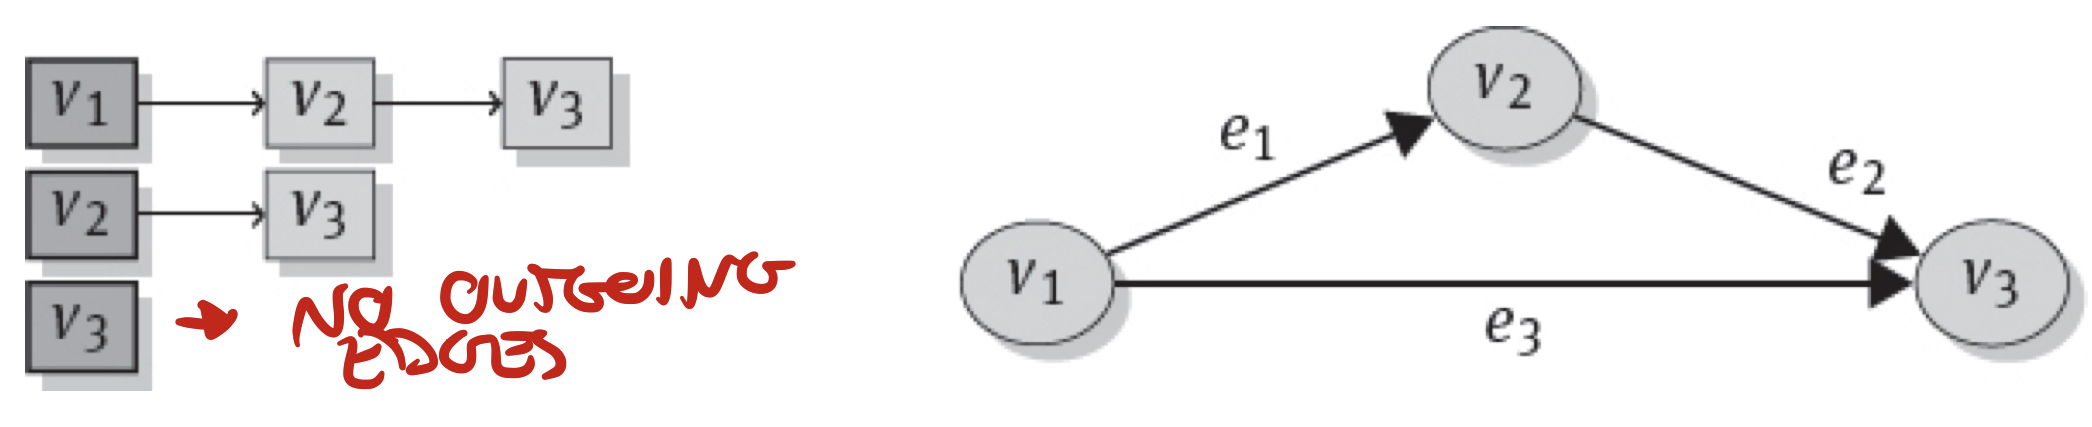
\includegraphics[width=0.7\linewidth]{images/AdvancedDataManagment/graph_databases/adj_list_simple_directed.jpeg}
        \end{figure}
    
    
    \item \textbf{Multigraphs:} in both the directed as well as the undirected case, nodes can occur multiple times in an adjacency list
    \begin{figure}[!h]
        \centering
        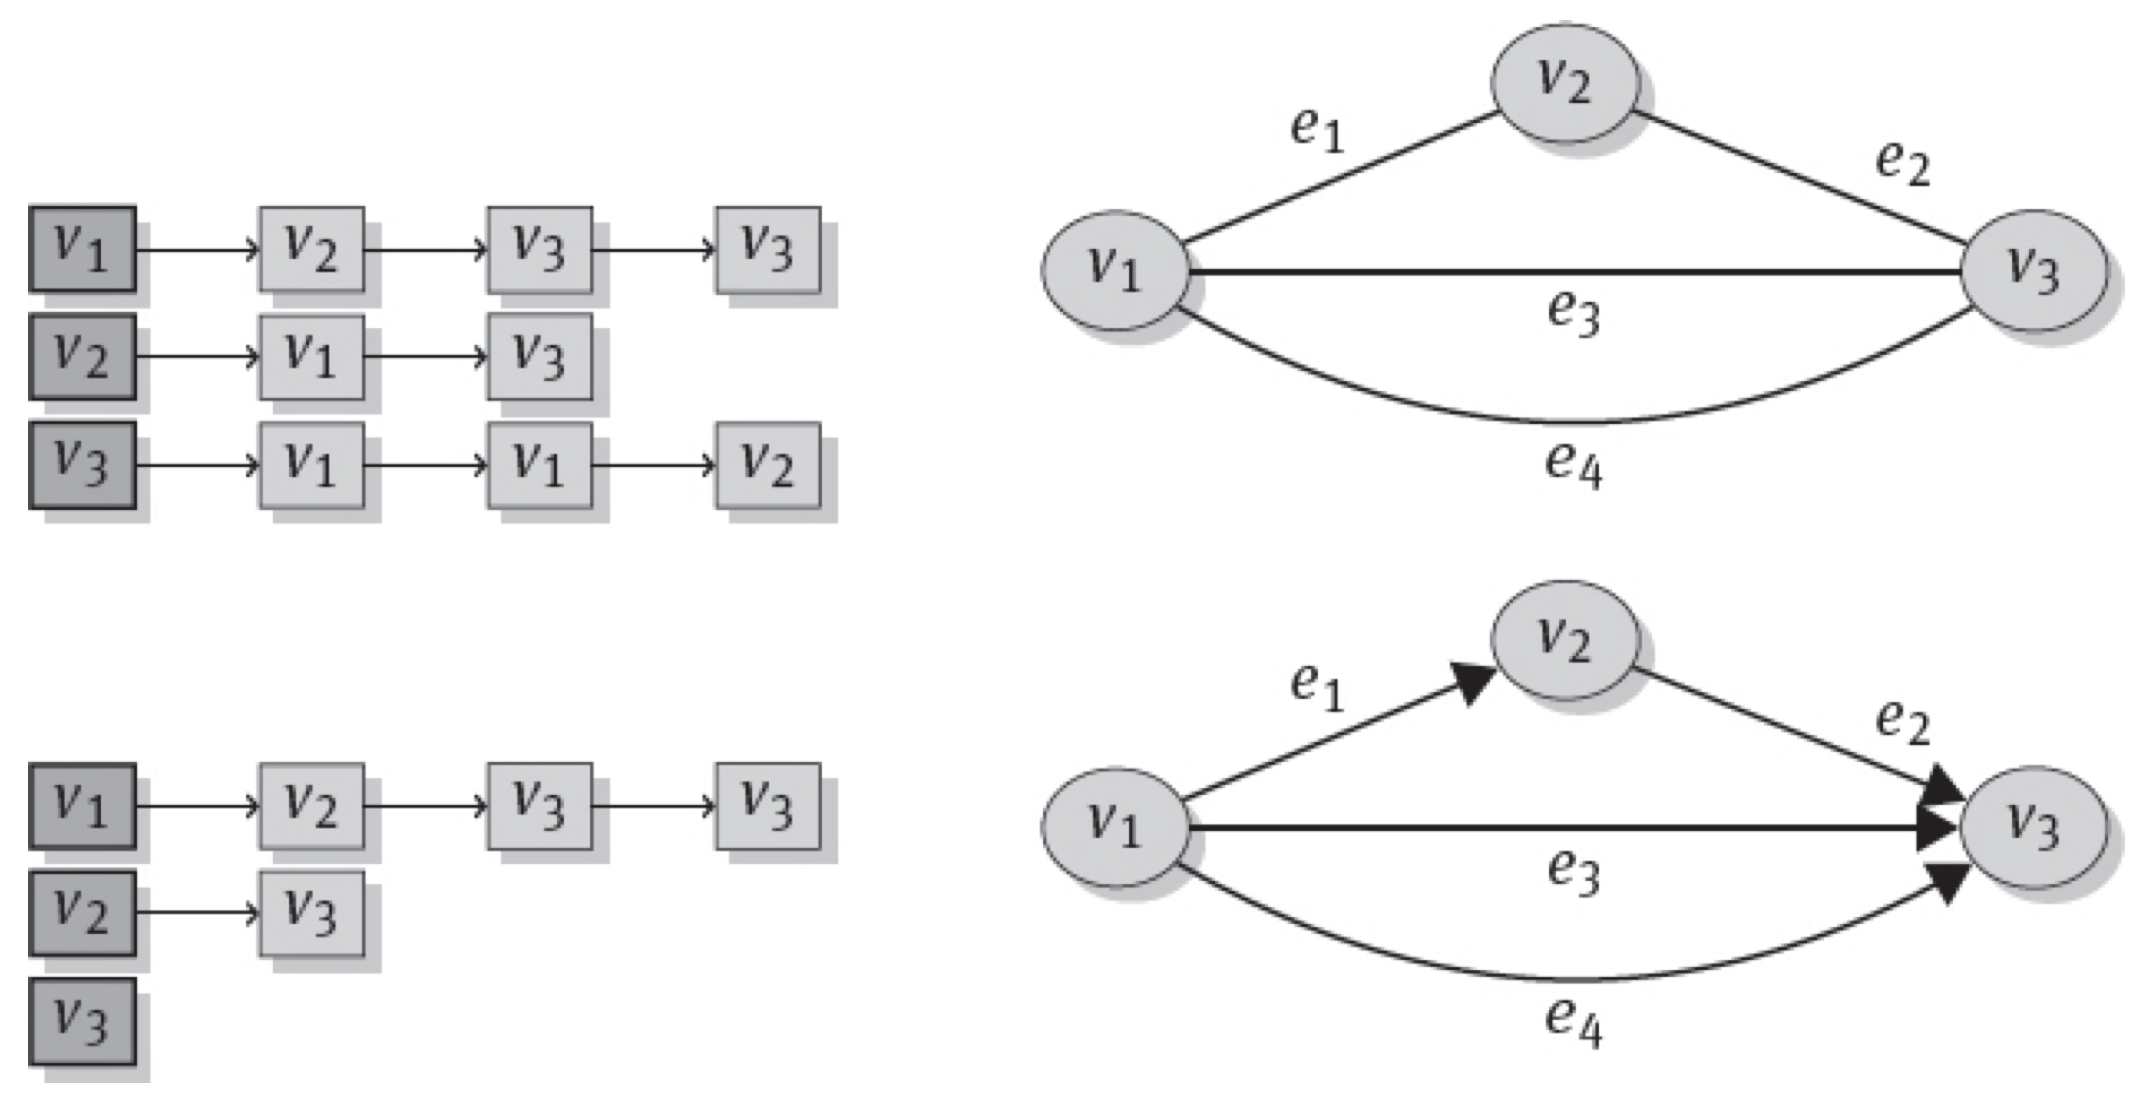
\includegraphics[width=0.7\linewidth]{images/AdvancedDataManagment/graph_databases/adj_list_multi.jpeg}
        \end{figure}
    
\end{itemize}
\subsubsection{Advantages}
\begin{itemize}
    \item Quick insertion of new vertices and edges
    \item Quick lookup of all neighboring vertices
    \item No storage overhead occurs
    \item Hyperedges can be stored
\end{itemize}

\subsubsection{Disadvantages}
\begin{itemize}
    \item Checking existence of a single edge requires a full scan of the adjacency list of the source node
\end{itemize}

\subsection{Incidence List}
With an incidence list, you store the \textbf{vertex set} \(V\) and for each vertex you store a \textbf{linked list of incident edges}
\begin{itemize}
    \item When the edge is \textit{directed} the edge object contains information on its \textbf{source} node and its \textbf{target node}
    \item When the edge is \textit{undirected} no difference is made between source and target nodes
\end{itemize}
\begin{itemize}
    \item \textbf{Simple undirected graph:} each undirected edge is contained in the incidence lists of its two connected nodes
    \begin{figure}[!h]
        \centering
        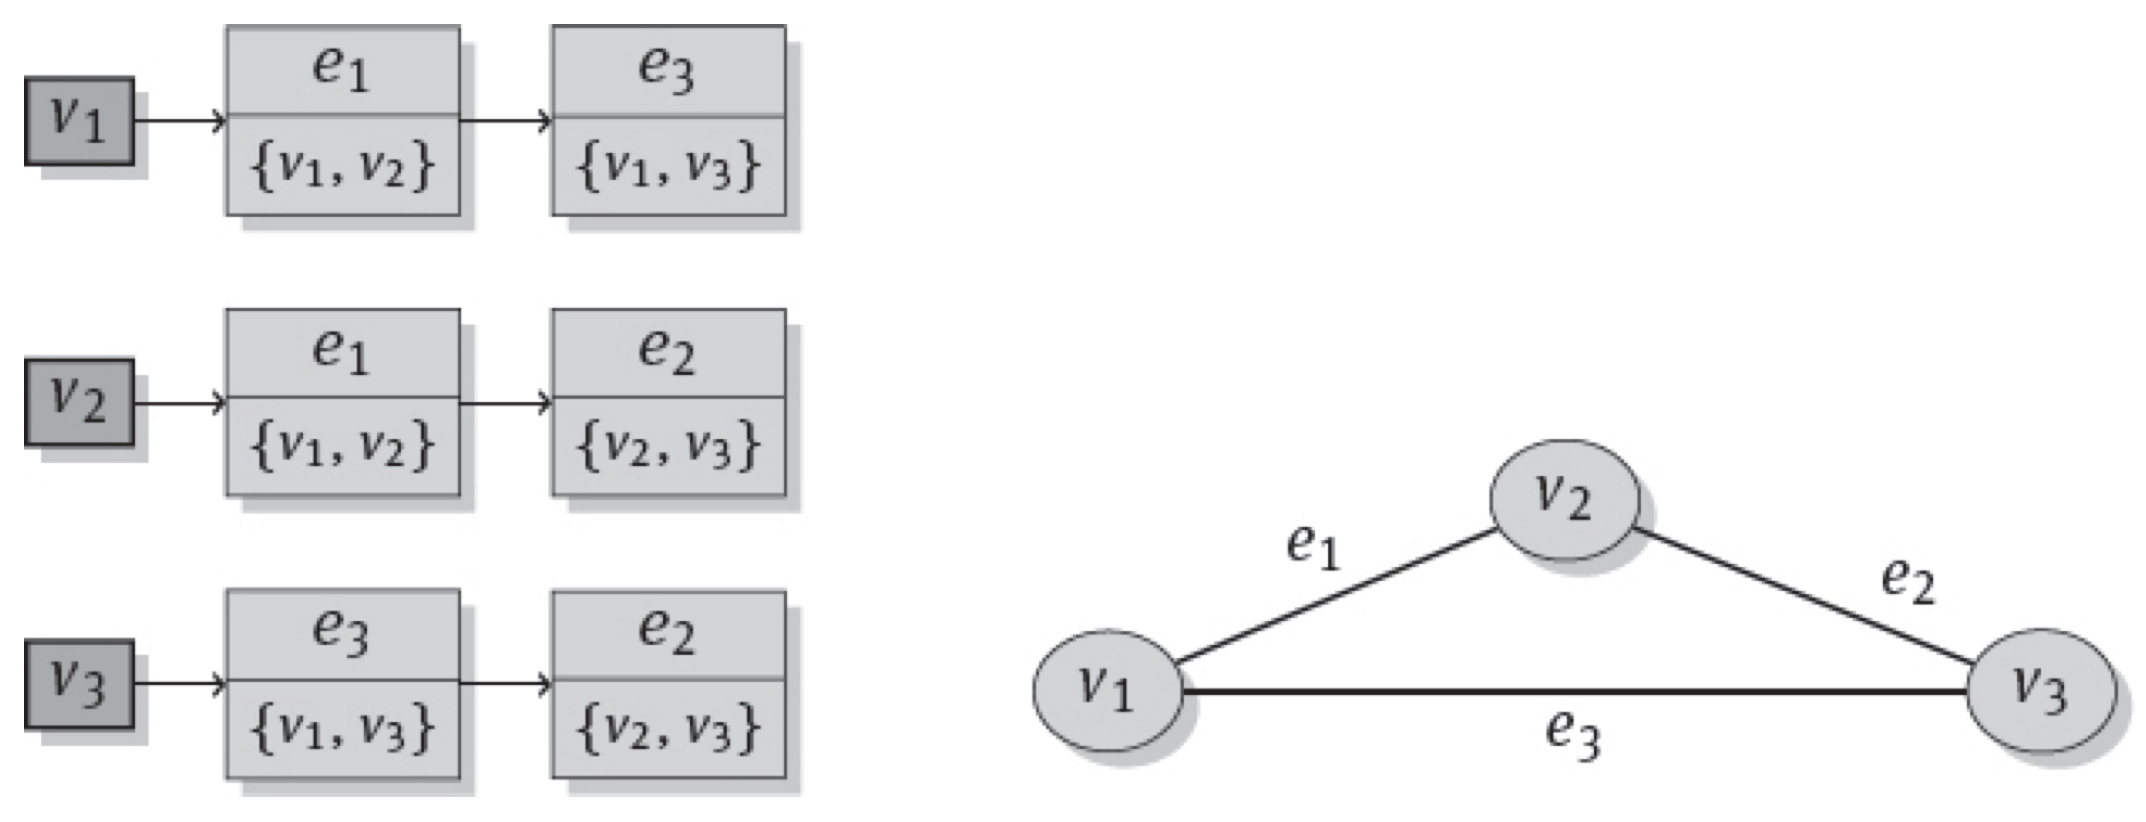
\includegraphics[width=0.7\linewidth]{images/AdvancedDataManagment/graph_databases/inc_list_simple_undirected.jpeg}
        \end{figure}
    
    \item \textbf{Simple directed graph:} it suffices to store only outgoing edges in the incidence list as long as only a forward traversal of the edges is needed. In this case, it is advantageous to store all incident edges in a node’s incidence list to allow for both forward traversal of the outgoing edges and backward traversal of the incoming edges. We could have two incidence list>
    \begin{itemize}
        \item One for the \textbf{outgoing} edges for the forward traversal
        \item One for the \textbf{incoming} edges for the backword traversal
    \end{itemize}
    \begin{figure}[!h]
        \centering
        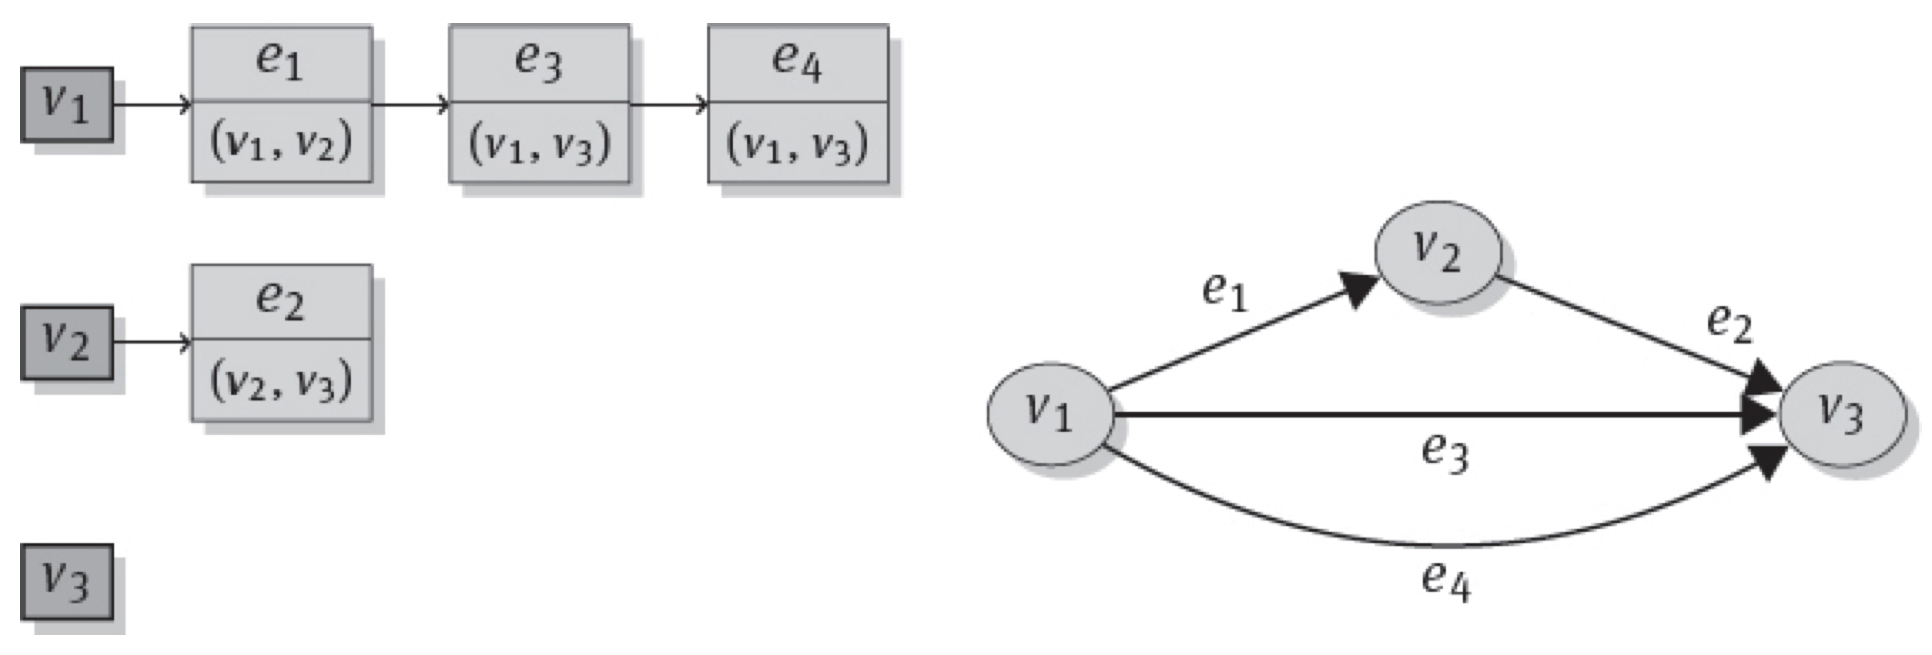
\includegraphics[width=0.7\linewidth]{images/AdvancedDataManagment/graph_databases/inc_list_simple_directed.jpeg}
        \end{figure}
    
    \item \textbf{Multigraphs:} in both directed as well as the undirected case, each edge has its own identity and hence is stored separately.
    \begin{itemize}
        \item For the \textbf{undirected} case each edge contains pointer to the incident nodes
        \begin{figure}[!h]
        \centering
        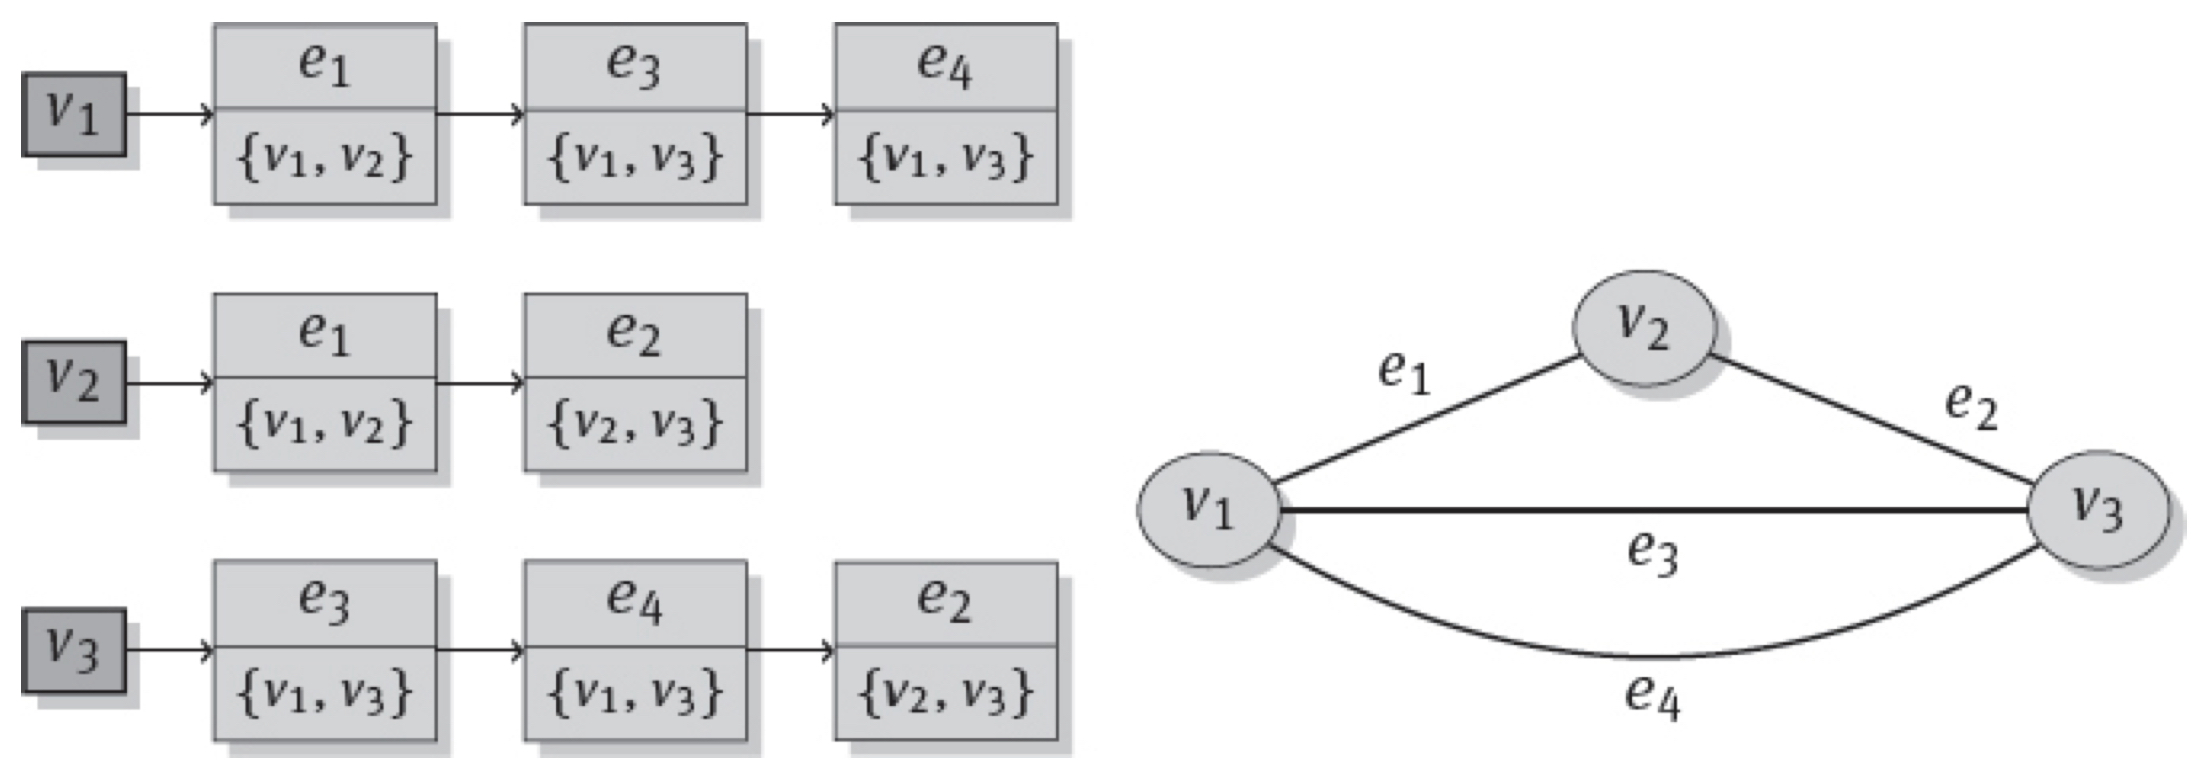
\includegraphics[width=0.7\linewidth]{images/AdvancedDataManagment/graph_databases/inc_list_multi_undirected.jpeg}
        \end{figure}
        \newpage
        \item For the \textbf{directed} case each edge would have a pointer to its source node as well as one pointer to its target node
        \begin{figure}[!h]
        \centering
        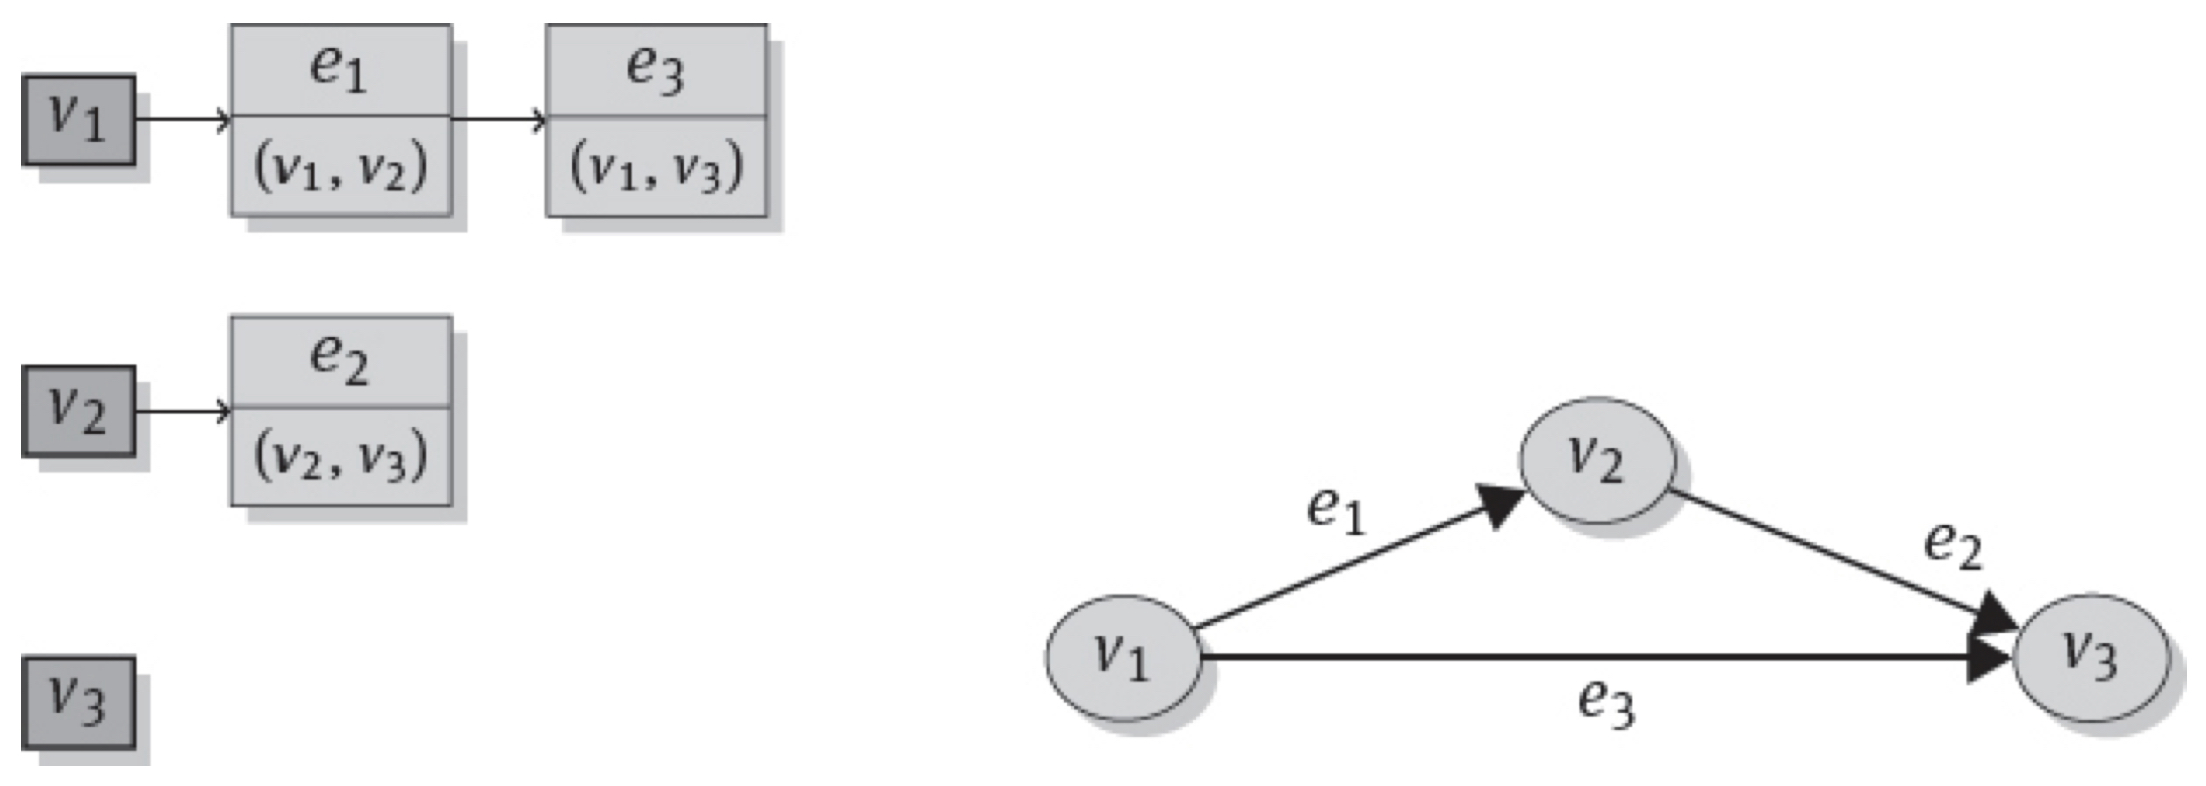
\includegraphics[width=0.7\linewidth]{images/AdvancedDataManagment/graph_databases/inc_list_multi_directed.jpeg}
        \end{figure}
    \end{itemize}
\end{itemize}
In practical implementations, the incidence list would be \textbf{stored inside a node object} as a \textbf{collection of pointers} to incident edge objects – potentially – in the directed case – one collection for incoming and one collection for outgoing edges to allow for both forward and backward traversal.

\section{The Property Graph Model}
\begin{itemize}
    \item The basic storage structure usually is a directed multigraph
    \item We must be able to \textbf{store information} inside the \textit{node} as well as along the \textit{edges}
    \item We must be able to distinguish different kind of nodes and edges. Point achieved by the \textbf{multi-relational} graph where \textbf{types} are introduced for nodes and edges.
    \begin{itemize}
        \item Each node is labeled with the \textbf{node label} that correspond to the node type
        \item Each edge is labeled with the \textbf{edge label} that correspond to the edge type
    \end{itemize}
    \item A type defines \textbf{attributes} for the corresponding nodes and edges. So an attribute definition must contain a name for the attribute and it mus specify a domain of values
    \item Like \textit{name:value} pairs describe \textbf{proprieties} of a node or edge
    \item \textbf{Edge labels} between any two nodes should be \textbf{unique}
    \item Each node has a system-defined \textbf{unique identifier}
\end{itemize}
A propriety graph \(G\) can be defined as \(G = (V, E, L_V, L_E, ID)\):
\begin{itemize}
    \item \(V\) set of \textbf{nodes}
    \item \(E\) set of \textbf{edges}
    \item \(L_V\) set of \textbf{node labels} st to each label \(l \in L_E\) we can assign a set of attribute definitions
    \item \(L_E\) set of \textbf{edge labels} st to each label \(l \in L_E\) we can assign a set of attribute definitions
    \item \(ID\) set of identifiers that can uniquely be assigned to nodes and edges
\end{itemize}
A specific node \(v \in V\) has the following definition: \(v = (id, l, P)\):
\begin{itemize}
    \item \(id \in ID\)
    \item \(l \in L_V\)
    \item \(P\) is a set of proprieties, st each \textbf{propriety} \(p \in P\) is a \textit{name:value}-pair st:
    \begin{itemize}
        \item The \textit{name} correspond to an attribute name defined by the node type
        \item The \textit{value} is a valid value taken from the teh attribute domain
    \end{itemize}
\end{itemize}
Similarly an edge \(e \in E\) is defined like so \(e = (id, l', P, source, target)\):
\begin{itemize}
    \item \(l'\) is an edge label from \(L_E\)
    \item The proprieties in \(P\) correspond to an attribute definitions of this edge type
\end{itemize}

\subsubsection{Example}
\begin{figure}[!h]
        \centering
        \includegraphics[width=0.7\linewidth]{images/AdvancedDataManagment/graph_databases/propriety_graph_example.jpeg}
        \caption{A property graph for a social network}
        \end{figure}
\begin{itemize}
    \item The node set is \(V = \{v_1, v_2, v_3\}\)
    \item The edge set is \(E = \{e_1, e_2, e_3\}\)
    \item The node labels are \(L_V = \{Person\}\)
    \item The node type definitions are \(t_{Person} = \{Person, A_{Person}\}\) where the attribute definitions are \textit{APerson} = \textit{\{(Name, String), (Age, Integer)\}}
    \item The edge labels are \(L_E = \{knows, dislikes\}\)
    \item The edge type definitions are \(t_{knows} = \{knows, A_{knows}, \{Person\}, \{Person\}\}\) and \(t_{dislikes} = \{dislikes, \emptyset, \{Person\}, \{Person\}\}\), where \textit{Aknows = \{(since, Date)\}}
\end{itemize}
The specification of nodes and edges are the following:
\begin{itemize}
    \item \(v_1 =\) \textit{\{1, Person, \{Name: Alice, Age: 34\}\}}
    \item \(v_2 =\) \textit{\{2, Person, \{Name: Bob, Age: 27\}\}}
    \item \(v_3 =\) \textit{\{3, Person, \{Name: Charlene, Age: 29\}\}}
    \item \(e_1 =\) \textit{\{4, knows, \{since: 31-21-2009\}, 1, 2\}}
    \item \(e_2 =\) \textit{\{5, knows, \{since: 10-04-2011\}, 2, 3\}}
    \item \(e_3 =\) \textit{\{6, dislikes, ;, 1, 3\}}
\end{itemize}

In addition we specify an additional requirement: \textbf{there may never be two edges with the same label between two nodes.} Like the following example
\begin{figure}[!h]
    \centering
    \includegraphics[width=0.7\linewidth]{images/AdvancedDataManagment/graph_databases/violation_example.jpeg}
    \caption{Violation of uniqueness of edge labels}
\end{figure}

\chapter{Distributed Databases}
For several decades, centralized database management systems running on a single database server have been predominant, for these four main reasons:
\begin{itemize}
    \item \textit{Complexity} of a single-server system was lower and administration easier
    \item \textit{Evaluate short queries} and \textit{infrequent data modification}
    \item \textit{Slow network} so sending large amount of data was too costly
    \item \textit{Parallelization} required rewriting a query into subqueries and recombining the results, overhead diminished the positive effects of a parallel execution of subqueries
\end{itemize}
Whenever there were more demanding requirements:
\begin{itemize}
    \item \textbf{Scaling up} or \textbf{Vertical scaling} equip the single database server with higher hardware capacity
    \begin{itemize}
        \item Amount of data and queries a single database server can handle is limited
        \item A single server is always a single point of failure
    \end{itemize}
    \item \textbf{Scaling out} or \textbf{Horizontal scaling} connecting several cheaper servers in a network
    \begin{itemize}
        \item The only option to improve the throughput and latency of a database system
        \item Disadvantage of cost of coordination and synchronization of the database servers
        \item However this last one pays off for large scale systems or global enterprises with several data centers
    \end{itemize}
\end{itemize}

\section{Scaling Horizontally}
\begin{itemize}
    \item The ability of a database system to \textit{flexibly scale out by distributing data in a server network} is called \textbf{horizontal scalability}
    \item Servers can work independently
    \item Also called \textbf{shared-nothing architecture}
    \item The most common use case today is a distributed database on a shared-nothing architecture
    \begin{itemize}
        \item A distributed database management system (DDBMS) that runs on a network of independent servers
        \item The servers need not be large
        \item They consist of cheaper commodity hardware so that each server can easily be replaced by a new one
    \end{itemize}
\end{itemize}
DBMS are benefical also when aiming for improved availability and reliability in smaller scaled systems:
\begin{itemize}
    \item \textbf{Load balancing:} user queries and other processes should be assigned to the servers in the network such that all servers have approximately the same load
    \item \textbf{Flexible scalability:} servers may flexibly leave and join the network at any time
    \item \textbf{Heterogeneous nodes:} servers may flexibly leave and join the network at any time
    \item \textbf{Symmetric configuration:} every node is configured identically to the others;
    \item \textbf{Decentralized control:} peer-to-peer algorithms for data management improve failure tolerance of a DDBMS
\end{itemize}

\section{Distribution Transparency}
For a user it must basically be transparent how the DBMS internally handles data storage and query processing in a distributed manner.
\begin{itemize}
    \item \textbf{Access transparency:} uniform query and management interface to users independent of the structure of the network
    \item \textbf{Location transparency:} the distribution of data in the database system is hidden from the user
    \item \textbf{Replication transparency:} if several copies of a data item are stored on different servers the user should not be aware of this
    \item \textbf{Fragmentation transparency:} if a large data set has to be split into several data items and the distributed database system does this splitting internally and the user can query the database as if it contained the entire unfragmented data set
    \item \textbf{Migration transparency:} if data items have to be moved from one server to another, this should not affect how a user accesses the data
    \item \textbf{Concurrency transparency:} when multiple users access the database system, their operation must not interfere or lead to incorrect data in the database system
    \item \textbf{Failure transparency:} as a distributed database system is more complex than a centralized one
\end{itemize}

\section{Failures in Distributed Systems}
\begin{itemize}
    \item \textbf{Server failure:} a DBS may fail to process messages due to notwork component crash or a self crash
    \begin{figure}[!h]
        \centering
        \includegraphics[width=0.2\linewidth]{images/AdvancedDataManagment/distributed_databases/server_failure.jpeg}
    \end{figure}
    
    \item \textbf{Message failures:} message through the network links may be delayed or lost during times of high congestion
    \item \textbf{Link failure:} a communication link between two servers may be unable to transmit messages. Note that a \textit{link failure} \textbf{can cause} a \textit{message failure}
    \begin{figure}[!h]
        \centering
        \includegraphics[width=0.2\linewidth]{images/AdvancedDataManagment/distributed_databases/link_failure.jpeg}
    \end{figure}
    \item \textbf{Network partition:} when the network is splitted into two or more subnetworks that are unable to communicate
    \begin{figure}[!h]
        \centering
        \includegraphics[width=0.2\linewidth]{images/AdvancedDataManagment/distributed_databases/network_partition.jpeg}
    \end{figure}
\end{itemize}

\textbf{Node Failure} can be categorized into:
\begin{itemize}
    \item \textbf{Crash failures:} is a permanent failure of a server and corresponds to aborting a communication protocol. Once the server crashed, it will never resume operation
    \item \textbf{Omission failures:} an omission failure corresponds to not taking some action
    \item \textbf{Commission failures:} corresponds to taking an action that is not correct according to  a communication protocol
\end{itemize}
Moreover we note that:
\begin{itemize}
    \item Crash failures are a special case of omission failures.
    \item The union of omission and commission failures is called \textbf{Byzantine failures}
    \item The term \textbf{non-Byzantine failures} usually refers to omission failures but in addition explicitly also covers duplication and reordering of messages
\end{itemize}

Distributed DBMSs have to provide a high level of \textbf{fault tolerance}, indeed, a distributed system may in general be design based on a certain \textbf{failure model} which describes the set of failures that the system can tolerate.
\begin{itemize}
    \item \textbf{Fail-stop model:} all server failures are crash failures that permanently render the server unavailable 
    \item \textbf{Fail-recover model:} a server may halt but it may later resume execution. The resumption could be:
    \begin{itemize}
        \item In the state before it was halted
        \item From scratch
    \end{itemize}
\end{itemize}

\section{Epidemic Protocols and Gossip Communication}
Due to the many properties  the propagation of information in the network is difficult to manage. In the \textit{simplest scenario} 
\begin{itemize}
    \item Whenever new information is received by one server, the server sends a notification to all the other servers he know
    \item But the initiating server might not be aware of all servers currently in the network
    \item Some of his messages might be lost due to network failures
\end{itemize}
\begin{tcolorbox}
An alternative is when the DBS can be seen as participants in a \textit{peer-to-peer network} where there is \textit{no central coordinator}. \textbf{Epidemic protocols} are a category of peer-to-peer algorithms, where information is spread like an infection all over the network
\end{tcolorbox}
An other application is \textbf{membership} of peers n the network:
\begin{itemize}
    \item Each server has to maintain a list of names
    \item This list can be kept up-to-date by an epidemic algorithm
    \item Servers exchange their membership lists in a peer-to-peer fashion so that the information which servers are part of the network slowly spreads over the entire network
\end{itemize}
With an epidemic algorithm, servers in the network pass on a message \textbf{like an infection}. A \textbf{message} notification that some new server has joined the network, so the servers that receive this message update their membership list.
We have three types of nodes:
\begin{itemize}
    \item \textbf{Infected nodes:} are servers that have received a new message that they want to pass on to others
    \item \textbf{Susceptible nodes:} are nodes that so far have not received the new message
    \item \textbf{Removed nodes:} are nodes that already have received the message but are no longer willing to pass it
\end{itemize}

There are three different communication modes that can be applied in epidemic algorithms:
\begin{itemize}
    \item \textbf{push-only:} an infected server contacts another server and passes on all the new messages it has received. Infected server \(\rightarrow\) susceptible server
    \item \textbf{pull-only:} a susceptible server contacts another server and asks for new messages. Susceptible server \(\rightarrow\) infected server
    \item \textbf{push-pull:} one server contacts another server and both
exchange their new messages. Both servers have the same state
\end{itemize}

A synonym for epidemic message exchange is \textbf{gossiping:} the term expresses that messages spread in a server network like rumors in human communication.

Two variants of epidemic algorithms for database updates are:
\begin{itemize}
    \item \textbf{Anti-entropy} is a periodic task that is scheduled for a fixed time span, for example every minute. It is called also \textit{simple epidemic} since any server is either susceptible or infective and the infection process \textit{does not degrade} over time or due to some probabilistic decision.
    \item \textbf{Rumor spreading} is an infection that can be triggered by the \textit{arrival of a new message} or it can be run periodically. Here the infection have several rounds, in each one a server chooses a set of communication partners (called \textit{fanout}). It is a \textit{complex epidemic} because infection of other servers is a dynamic process: amount of server decreases every round.
\end{itemize}
This decrease of infections can be varied as follows:
\begin{itemize}
        \item \textit{Probabilistic:} after each exchange with another server, the server stops being infective with a certain probability
        \item \textit{Counter-based:} After a certain number k of exchanges, the server stops being infective. Therer are two cases:
        \begin{itemize}
            \item \textit{Infect-and-die} the number k is equal to the fan-out
            \item \textit{Infect-forever} the number k is infinite and the server never stops
        \end{itemize}
        \item \textit{Blind:} the server becomes removed without taking the feedback of communication partners is into account
        \item \textit{Feedback-based:} the server becomes removed if it notices that the communication partners already have received the new message
    \end{itemize}
    
\subsection{Hash Trees}
A major issue with epidemic protocols is how two servers can identify those messages in which they differ. For example a complete comparison of all messages is not feasible as this would slow down the epidemic process tremendously.

A simple improvement is to use a \textbf{list of hash values}
\begin{itemize}
    \item Comparison of hash values is faster
    \item The downside, the hash values have to be computed and still the list of hash values has to be compared sequentially
\end{itemize}
A step further could be take using a \textbf{hash tree}:
\begin{itemize}
    \item It starts with a hash of each message in a leave node, and then iteratively concatenates hashes
    \item For \textit{inner node}, closer a hash value is to the root, the more leave it covers
    \item The last hash value at the root of the tree is called the \textbf{top hash}
\end{itemize}

\begin{figure}[!h]
        \centering
        \includegraphics[width=0.85\linewidth]{images/AdvancedDataManagment/distributed_databases/hash_tree.jpeg}
        \caption{A hash tree for four messages}
    \end{figure}
Now, with a hash tree, message list comparison is improved:
\begin{itemize}
    \item When the two top hashes are identical, the two message lists are identical
    \item If the top hashes differ, we go the the next level of the tree and compare the hash values there identical
    \item Whenever we encounter an inner node that has identical hash values in the two hash trees under comparison, then we know that the messages below this inner node are identical
    \item As long as hash values differ for an inner node, we have to go one level deeper and compare the hash values of the child nodes
    \item When we reach a leaf node with different hash values, we have identified a message on which the two message lists differ
\end{itemize}
\newpage
In order to avoid unnecessary hash comparisons, we have to ensure identical root hashes for identical message list. And could be done by:
\begin{itemize}
    \item Let the two servers agree on a sorting order, sort all messages according to this order and then compute the hash tree just before the comparison
    \item Or make each server precompute hash trees for any possible sorting order of the messages. And for comparison the servers then just have to find those two trees with the same sorting order
\end{itemize}

\chapter{Data Fragmentation}
In a distributed database system, two major questions are:
\begin{itemize}
    \item How the entire set of data items in the database can be split into subsets \(\rightarrow\) \textbf{ data fragmentation (sharding / partitioning)}
    \item How the subsets can be distributed among the database servers in the network \(\rightarrow\) \textbf{data allocation}
\end{itemize}

\section{Properties and Types of Fragmentation}
The query behavior of users plays an important role for the quality of fragmentation and allocation, like the:
\begin{itemize}
    \item Type of access
    \item Access patterns
    \item Affinity of records
    \item Frequency of accesses 
    \item Accesses duration
\end{itemize}
Once a good fragmentation and allocation have been established, a distributed database can take \textbf{advantage} of:
\begin{itemize}
    \item Data locality
    \item Minimization of communication costs
    \item Improved efficiency of data management
    \item Load balancing 
\end{itemize}
However on average a fragmented database system has to live with several \textbf{disadvantages}:
\begin{itemize}
    \item Queries that involve subqueries over different fragments are costly because the global query has to be split into subqueries
    \item Distributed transactions are extremely difficult to manage
\end{itemize}
Several criteria are important when designing a distributed database with fragmented data sets. The most important is that a given data fragmentation must be correct, in the sense that the original data must be \textit{entirely reconstructed}. When the data set is recombined from the fragments, the following two \textbf{correctness properties} are required:
\begin{itemize}
    \item \textbf{Completeness:} none of the original data records is lost during fragmentation and hence no data is missing in the reconstructed data set
    \item \textbf{Soundness:} no additional data are introduced in the reconstructed data set
\end{itemize}

\section{Data Allocation}
For fragmented data a major problem is how to \textit{distribute the fragments} over the database servers. A \textbf{data allocation mechanism} has to decide which fragment should be stored on which server, thus \textbf{load balancing} has to be taken into account. There are several forms of data allocation:
\begin{itemize}
    \item \textbf{Range-based allocation} relies on range-based fragmentation. When a range-based fragmentation is obtained the identified ranges have to be assigned to the available servers
    \item \textbf{Hash-based allocation} uses a hash function on the input fragments to determine which server each fragment is assigned to. With hash-based allocation the distribution of the records among the servers is usually more balanced because the hash function distributes its input values well over its entire output hash values
    \item \textbf{Cost-based allocation} describes the data allocation task as an optimization problem
\end{itemize}

\subsection{Consistent Hashing}
Consistent hashing is an hash-based allocation schema which provides a better and more flexible distribution of the records among a set of servers.
\begin{itemize}
    \item A hash function is computed on each input fragment
    \item The hash values are now seen as a ring that wraps around: when we have reached the highest hash value we start again from 0
    \item A hash value is computed not only for each fragment but also for each database server
\end{itemize}
By computing a hash value for a database server, \textbf{each server} has a \textit{fixed position on the ring}; the advantage of these hash values is that they presumably distribute the servers uniformly on the ring.
\newpage
\begin{tcolorbox}
A widely used allocation policy is then to store data on the next server on the ring when looking in clockwise direction.
\end{tcolorbox}
\begin{figure}[!h]
        \centering
        \includegraphics[width=0.4\linewidth]{images/AdvancedDataManagment/data_fragmentation/data_allocation.jpeg}
        \caption{Data allocation with consistent hashing}
    \end{figure}
A major advantage of consistent hashing is its \textit{flexible support} of \textbf{additions} or \textbf{removals} of servers.
\begin{itemize}
    \item Whenever a server \textbf{leaves} the ring: all the data that it stores have to be moved to the next server in clockwise direction
    \begin{figure}[!h]
        \centering
        \includegraphics[width=0.4\linewidth]{images/AdvancedDataManagment/data_fragmentation/server_removal.jpeg}
        \caption{Server removal with consistent hashing}
    \end{figure}
    \newpage
    \item Whenever a server \textbf{joins} the ring: the data with a hash value less than the hash value of the new server have to be moved to the new server
    \begin{figure}[!h]
        \centering
        \includegraphics[width=0.4\linewidth]{images/AdvancedDataManagment/data_fragmentation/server_addition.jpeg}
        \caption{Server addition with consistent hashing}
    \end{figure}
\end{itemize}
An important tool to make consistent hashing \textit{more flexible} is to have not only one location on the ring for each physical server but instead to have \textit{multiple locations}: these locations are then called \textbf{virtual servers}. Virtual servers improve consistent hashing in the following cases:
\begin{itemize}
    \item The virtual servers (of each physical server) are spread along the ring in an arbitrary way. So, all servers have a better spread on the ring which leads to a better data distribution
    \item Heterogeneous servers are supported. So a server with less capacity can be represented by less virtual servers than a server with more capacity
    \item New servers can be gradually added to the ring: instead of shifting its entire data load onto a new server at once, virtual servers for the new server can be added one at a time. In this way the new server has tie to start up slowly and take in its full load step by step until its full capacity is reached.
\end{itemize}
\begin{figure}[!h]
        \centering
        \includegraphics[width=0.4\linewidth]{images/AdvancedDataManagment/data_fragmentation/virtual_servers.jpeg}
        \caption{Virtual server with consistent hashing}
    \end{figure}

\chapter{Replication And Synchronization}
Replication refers to the concept of storing several copies of a data record at different database servers. These \textit{copies} are called \textbf{replicas} and the \textit{number of copies} is called the \textbf{replication factor}. 
When applying replication to large data sets:
\begin{itemize}
    \item First a fragmentation of the data set is obtained
    \item Fragments are replicated among a distributed database system
    \item Replication improves reliability and availability of a distributed system because replicas can serve as backup copies whenever one of the servers fails and becomes unavailable
    \item It enables load balancing or data locality
    \item This kind of concurrent accesses to different replicas lead to consistency problems
\end{itemize}

\section{Replication Models}
Replication has several \textbf{advantages:}
\begin{itemize}
    \item It improves the \textbf{reliability} by offering higher data availability
    \item It offers \textbf{lower latency} by enabling load balancing, data locality and parallelization
\end{itemize}
These two advantages implies respectively two a major \textbf{disadvantages}:
\begin{itemize}
    \item \textbf{Consistency problems}: because when a user updates a data record at one server, network delays or even network failures may prevent the database system from updating all other replicas of the data record quickly
    \item \textbf{Concurrency problem:} where two or more users might concurrently update the same data record on different replicas
\end{itemize}

\begin{tcolorbox}
The two basic models of replication are \textbf{master-slave} and \textbf{multi-master} replication. While the \textit{consistency problem} exists for both, the \textit{concurrency problem} is \textbf{avoided} in the \textbf{master-slave} case but at the cost of higher latency for write requests
\end{tcolorbox}

\subsection{Master-Slave Replication}
\begin{itemize}
    \item In master-slave replication, \textit{write} requests are handled only by a \textit{single server} that is called the \textbf{master}.
    \item After a write, the master is responsible for \textit{updating} all other servers that hold a replica, called \textbf{slaves}
    \item Read requests can be accepted by both the master and the slaves
\end{itemize}
\begin{figure}[!h]
        \centering
        \includegraphics[width=0.8\linewidth]{images/AdvancedDataManagment/replication_and_synchronization/master_slave_replication.jpeg}
        \caption{A Master-slave replication}
    \end{figure}

Master-slave replication offers enough \textbf{redundancy} in case of a \textbf{master failure}: when the master fails, \textit{one of the slaves} can be \textbf{elected} to be the \textbf{new master} and all write request are redirected to it.

Having a \textit{single master server} for all write requests in the database system is a \textbf{bottleneck} that slows down the processing of writes tremendously.
\begin{itemize}
    \item A solution is to \textit{partition} the set of all data records into \textbf{disjoint subsets} and to each such \textit{subset} assign \textit{one server} as the \textbf{master server}
    \item In combination with data partitioning, data records in the same partition are copied to the same replication servers and one of the servers is designated master for the entire partition while the others act as slaves
\end{itemize}
\begin{figure}[!h]
        \centering
        \includegraphics[width=0.8\linewidth]{images/AdvancedDataManagment/replication_and_synchronization/ms_rep_mul_records.jpeg}
        \caption{Master-slave replication with multiple records}
    \end{figure}


\subsection{Multi-Master Replication}
\begin{itemize}
    \item When all servers holding a replica of a data record can process write request, they all act as masters for the data record, this is the case of \textbf{multi-master replication} or \textbf{peer-to-peer replication} (based on the fact that the masters are peers with identical capabilities and they have to synchronize one with the other)
    \item Higher write availability than master-slave replication, because clients can contact any replica server with a write request, parallel requests
    %IMAGE
    \item All servers accept write and read requests for a data item
    \item The servers have to regularly synchronize their state among themselves
    \item Due to the \textbf{consistency problem:}
    \begin{itemize}
        \item Clients may retrieve \textit{outdated data} whenever the replica answering the client’s read request has \textit{not finished the synchronization process}
    \end{itemize}
    \item Due to the \textbf{concurrency problem:}
    \begin{itemize}
        \item Replicas may be in conflict when different clients wrote to different replicas without a synchronization
    \end{itemize}
\end{itemize}
\begin{figure}[!h]
        \centering
        \includegraphics[width=0.8\linewidth]{images/AdvancedDataManagment/replication_and_synchronization/multi_master_replication.jpeg}
        \caption{Multi-master replication}
    \end{figure}

\chapter{Polyglot DB Arch}
When designing the data management layer for an application, several of the identified database requirements may be contradictory. Regarding the data model, some data might be of a different structure than other data.

\section{Polyglot Persistence}
Instead of choosing \textit{just one single DBMS} to store the entire data, so-called \textbf{polyglot persistence} could be a viable option to satisfy all requirements towards a modern data management infrastructure.
\begin{itemize}
    \item It denotes that one can choose as many databases as needed so that all requirements are satisfied
    \item Optimal solution when backward-compatibility with a \textbf{legacy application} must be ensured
\end{itemize}
Polyglot persistence however comes with severe \textbf{disadvantages:}
\begin{itemize}
    \item There is no unique query interface or query language, thus there is not a unique database access method
    \item Cross-database consistency is a major challenge, and in case data are duplicated the duplicates have to be updated or deleted in unison
\end{itemize}
It should obviously be avoided to push the burden of all of these query handling and database synchronization task to the application level. Thus the \textit{integration layer} is introduces to take
care of processing queries.
\begin{itemize}
    \item Decomposing queries in to several subqueries
    \item Redirecting queries to the appropriate databases
    \item Recombining the results obtained from the accessed databases
\end{itemize}
Finally the \textit{integration layer} should ensure \textbf{cross-database consistency}: it must synchronize data in the different databases by propagating additions, modifications or deletions among them.
\begin{figure}[!h]
        \centering
        \includegraphics[width=0.7\linewidth]{images/AdvancedDataManagment/polyglot_database_architectures/polygot_pers.jpeg}
        \caption{Polyglot persistence with integration layer}
    \end{figure}


\section{Lambda Architecture}
When real-time (stream) data processing is a requirement, the combination of the following two features might be appropiate:
\begin{itemize}
    \item A slower batch processing layer
    \item A quiker stream processing layer
\end{itemize}
This architecture has been recently termed \textbf{lambda architecture}, it major feature is that it processes a continuous flow of data in the following three layers:
\begin{itemize}
    \item \textbf{Speed Layer} collects only the most recent data and as soon as data ave been included in the other two layers, it can be discarded from the speed layer. Moreover it computes results over its dataset and delivers teh results in several \textbf{real-time views}
    \item \textbf{Batch Layer} stores all data in an append-only and immutable way in a so-called \textit{master dataset}. It evaluates functions over the entire dataset; the results are delivered in so-called \textbf{batch views}
    \item \textbf{Serving Layer} makes batch views accessible to user queries
\end{itemize}
\begin{figure}[!h]
        \centering
        \includegraphics[width=0.7\linewidth]{images/AdvancedDataManagment/polyglot_database_architectures/lambda_arc.jpeg}
        \caption{Lambda architecture}
    \end{figure}


\newpage
\section{Multi-Model Databases}
Relying on different storage backends increases the overall complexity of the system and raises different problems, so it might be advantageous to use a database system that stores data in a single store but provides access to the data with different APIs. 
\begin{tcolorbox}
Databases offering this feature have been termed \textbf{multi-model} databases. They either support different data models directly inside the database engine or they offer layers for additional data models on top of a single-model engine
\end{tcolorbox}
\begin{figure}[!h]
        \centering
        \includegraphics[width=0.7\linewidth]{images/AdvancedDataManagment/polyglot_database_architectures/multimodel_db.jpeg}
        \caption{A multi-model database}
    \end{figure}

Several advantages come along with this single-database multi-model approach:
\begin{itemize}
    \item \textit{Reduced database administration:} maintaining a single database is easier
    \item \textit{Reduced user administration:} only one level of user management is necessary
    \item \textit{Integrated low-level components:} low-level database components can be shared between the different data models in a multi-model database
    \item \textit{Improved consistency:} it is a lot easier to ensure
    \item \textit{Reliability and fault tolerance:} backup just has to be set up for a single database
    \item \textit{Scalability:} data partitioning and data locality can best be configured in a single database system
    \item \textit{Easier application development:} programming efforts regarding database administration  data models and query languages can focus on a single database system
\end{itemize}

\part{Document Databases}

\chapter{MongoDB}
\section{Document}
MongoDB stores data records as BSON documents. BSON is a binary representation of JSON documents, though it contains more data types than JSON. 

\subsection{Document Structure}
The value of a field can be any of the BSON data types, including other documents, arrays, and arrays of documents. Field names are strings. Documents have the following restrictions on field names:
\begin{itemize}
    \item The field name \(\_id\) is reserved for use as a primary key; its value must be unique in the collection, is immutable, and may be of any type other than an array. If the \(\_id\) contains subfields, the subfield names cannot begin with a (\$) symbol.
    \item Field names cannot contain the null character.
    \item The server permits storage of field names that contain dots (.) and dollar signs (\$)
    \item 
\end{itemize}

\subsection{Dot Notation}
MongoDB uses the dot notation to access the elements of an array and to access the fields of an embedded document.
To specify or access a field of an embedded document with dot notation, concatenate the embedded document name with the dot (.) and the field name, and enclose in quotes

\subsection{Document Limitations}
Documents have the following attributes:
\begin{itemize}
    \item \textbf{Document Size Limit:} The maximum BSON document size is 16 megabytes.
    \item \textbf{Document Field Order:} Unlike JavaScript objects, the fields in a BSON document are ordered.
    \item \textbf{The \(\_id\) Field:} In MongoDB, each document stored in a collection requires a unique \_id field that acts as a primary key. If an inserted document omits the \_id field, the MongoDB driver automatically generates an ObjectId for the \_id field.
\end{itemize}

\subsection{Other Uses of the Document Structure}
\begin{itemize}
    \item \textbf{Query Filter Documents:} Query filter documents specify the conditions that determine which records to select for read, update, and delete operations. You can use \(<field>:<value>\) expressions to specify the equality condition and query operator expressions
    \item \textbf{Update Specification Documents:} Update specification documents use update operators to specify the data modifications to perform on specific fields during an update operation.
    \item \textbf{Index Specification Documents:} Index specification documents define the field to index and the index type
\end{itemize}

\section{Databases and Collections}
MongoDB stores data records as documents (specifically BSON documents) which are gathered together in collections. A database stores one or more collections of documents.

\subsection{Database}
In MongoDB, databases hold one or more collections of documents. If a database does not exist, MongoDB creates the database when you first store data for that database.

\subsection{Collections}
MongoDB stores documents in collections. Collections are analogous to tables in relational databases.
\begin{itemize}
    \item \textbf{Create a Collection:} If a collection does not exist, MongoDB creates the collection when you first store data for that collection.
    \item \textbf{Explicit Creation:} MongoDB provides the db.createCollection() method to explicitly create a collection with various options, such as setting the maximum size or the documentation validation rules.
    \item \textbf{Document Validation:} By default, a collection does not require its documents to have the same schema; i.e. the documents in a single collection do not need to have the same set of fields and the data type for a field can differ across documents within a collection.
    \item \textbf{Modifying Document Structure:} To change the structure of the documents in a collection, such as add new fields, remove existing fields, or change the field values to a new type, update the documents to the new structure.
    \item \textbf{Unique Identifiers:} Collections are assigned an immutable UUID. The collection UUID remains the same across all members of a replica set and shards in a sharded cluster.
\end{itemize}

\section{MongoDB Query API}
A document in MongoDB is a data structure composed of field and value pairs. Documents are stored as BSON which is the binary representation of JSON. This low level of abstraction helps you develop quicker and reduces the efforts around querying and data modeling. The document model provides several advantages, including:
\begin{itemize}
    \item Documents correspond to native data types in many programming languages.
    \item Embedded documents and arrays reduce need for expensive joins.
    \item Flexible schema. Documents do not need to have the same set of fields and the data type for a field can differ across documents within a collection.
\end{itemize}

\section{MongoDB CRUD Operations}
https://www.mongodb.com/docs/manual/crud/

\section{Aggregation Pipeline}
An aggregation pipeline consists of one or more stages that process documents:
\begin{itemize}
    \item Each stage performs an operation on the input documents. For example, a stage can filter documents, group documents, and calculate values.
    \item The documents that are output from a stage are passed to the next stage.
    \item An aggregation pipeline can return results for groups of documents. For example, return the total, average, maximum, and minimum values.
    \item The same stage can appear multiple times in the pipeline with these stage exceptions: \(\$out\), \(\$merge\), and \(\$geoNear\)
    \item To calculate averages and perform other calculations in a stage, use aggregation expressions that specify aggregation operators. You will learn more about aggregation expressions in the next section.
\end{itemize}

\subsection{Aggregation Pipeline Expressions}
Some aggregation pipeline stages accept an aggregation expression, which:
\begin{itemize}
    \item Specifies the transformation to apply to the current stage's input documents.
    \item Transform the documents in memory.
    \item Can specify aggregation expression operators to calculate values.
    \item Can contain additional nested aggregation expressions.
\end{itemize}

\section{Replication}
A replica set in MongoDB is a group of mongod processes that maintain the same data set. Replica sets provide redundancy and high availability, and are the basis for all production deployments.

\subsection{Redundancy and Data Availability}
Replication provides redundancy and increases data availability. With multiple copies of data on different database servers, replication provides a level of fault tolerance against the loss of a single database server.

In some cases, replication can provide increased read capacity as clients can send read operations to different servers. Maintaining copies of data in different data centers can increase data locality and availability for distributed applications. You can also maintain additional copies for dedicated purposes, such as disaster recovery, reporting, or backup.

\subsection{Replication in MongoDB}
\begin{itemize}
    \item A replica set is a group of mongod instances that maintain the same data set.
    \item  A replica set contains several data bearing nodes and optionally one arbiter node.
    \item Of the data bearing nodes, one and only one member is deemed the primary node, while the other nodes are deemed secondary nodes.
    \begin{itemize}
        \item The \textbf{primary node} receives all write operations.
        \item The \textbf{secondaries} replicate the primary's oplog and apply the operations to their data sets such that the secondaries' data sets reflect the primary's data set. If the primary is unavailable, an eligible secondary will hold an election to elect itself the new primary. 
    \end{itemize}
\end{itemize}

\subsection{Asynchronous Replication}
Secondaries replicate the primary's oplog and apply the operations to their data sets asynchronously. By having the secondaries' data sets reflect the primary's data set, the replica set can continue to function despite the failure of one or more members.

\subsubsection{Replication Lag and Flow Control}
Replication lag refers to the amount of time that it takes to copy (i.e. replicate) a write operation on the primary to a secondary. Some small delay period may be acceptable, but significant problems emerge as replication lag grows, including building cache pressure on the primary.

\subsection{Automatic Failover}
When a primary does not communicate with the other members of the set for more than the configured electionTimeoutMillis period, an eligible secondary calls for an election to nominate itself as the new primary. The cluster attempts to complete the election of a new primary and resume normal operations.

The replica set cannot process write operations until the election completes successfully. The replica set can continue to serve read queries if such queries are configured to run on secondaries while the primary is offline.

Lowering the electionTimeoutMillis replication configuration option from the default 10000 (10 seconds) can result in faster detection of primary failure. However, the cluster may call elections more frequently due to factors such as temporary network latency even if the primary is otherwise healthy.

\section{Read Operations}
By default, clients read from the primary [1]; however, clients can specify a read preference to send read operations to secondaries.
\begin{itemize}
    \item \textbf{Asynchronous replication:} to secondaries means that reads from secondaries may return data that does not reflect the state of the data on the primary.
    \item \textbf{Multi-document transactions:} hat contain read operations must use read preference primary. All operations in a given transaction must route to the same member.
\end{itemize}

\subsection{Data Visibility}
\begin{itemize}
    \item Depending on the read concern, clients can see the results of writes before the writes are durable.
    \item For operations in a multi-document transaction, when a transaction commits, all data changes made in the transaction are saved and visible outside the transaction. That is, a transaction will not commit some of its changes while rolling back others.
    \item Until a transaction commits, the data changes made in the transaction are not visible outside the transaction.
\end{itemize}

\subsection{Mirrored Reads}
Mirrored reads reduce the impact of primary elections following an outage or planned maintenance. After a failover in a replica set, the secondary that takes over as the new primary updates its cache as new queries come in.

\subsection{Transactions}
Multi-document transactions that contain read operations must use read preference primary. All operations in a given transaction must route to the same member.

\section{Sharding}
Sharding is a method for distributing data across multiple machines. MongoDB uses sharding to support deployments with very large data sets and high throughput operations. There are two methods for addressing system growth: vertical and horizontal scaling.
\begin{itemize}
    \item \textbf{Vertical Scaling:} involves increasing the capacity of a single server, such as using a more powerful CPU, adding more RAM, or increasing the amount of storage space.
    \item \textbf{Horizontal Scaling:} involves dividing the system dataset and load over multiple servers, adding additional servers to increase capacity as required.
    \begin{itemize}
        \item Better efficiency than a single high-speed high-capacity server
        \item Expanding the capacity of the deployment only requires adding additional servers, so lower cost
    \end{itemize}
\end{itemize}

\subsection{Sharded Cluster}
A MongoDB sharded cluster consists of the following components:
\begin{itemize}
    \item \textbf{shard:} Each shard contains a subset of the sharded data. Each shard can be deployed as a replica set.
    \item \textbf{mongos:} The mongos acts as a query router, providing an interface between client applications and the sharded cluster.
    \item \textbf{config servers:} Config servers store metadata and configuration settings for the cluster.
\end{itemize}

\subsection{Shard Keys}
MongoDB uses the shard key to distribute the collection's documents across shards. The shard key consists of a field or multiple fields in the documents.
\begin{itemize}
    \item You select the shard key when sharding a collection.
    \item A document's shard key value determines its distribution across the shards.
\end{itemize}
\subsubsection{Shard Key Index}
To shard a populated collection, the collection must have an index that starts with the shard key.

\subsubsection{Shard Key Strategy}
The choice of shard key affects the performance, efficiency, and scalability of a sharded cluster. A cluster with the best possible hardware and infrastructure can be bottlenecked by the choice of shard key.

\subsection{Advantages of Sharding}
\begin{itemize}
    \item \textbf{Reads / Writes}: MongoDB distributes the read and write workload across the shards in the sharded cluster, allowing each shard to process a subset of cluster operations.
    \item \textbf{Storage Capacity:} Sharding distributes data across the shards in the cluster, allowing each shard to contain a subset of the total cluster data. 
    \item \textbf{High Availability:} The deployment of config servers and shards as replica sets provide increased availability.
\end{itemize}

\subsection{Considerations Before Sharding}
\begin{itemize}
    \item Sharded cluster infrastructure requirements and complexity require careful planning, execution, and maintenance.
    \item Once a collection has been sharded, MongoDB provides no method to unshard a sharded collection.
    \item While you can reshard your collection later, it is important to carefully consider your shard key choice to avoid scalability and perfomance issues.
\end{itemize}

\subsection{Sharded and Non-Sharded Collections}
A database can have a mixture of sharded and unsharded collections. Sharded collections are partitioned and distributed across the shards in the cluster. Unsharded collections are stored on a primary shard. Each database has its own primary shard.

\subsection{Connecting to a Sharded Cluster}
You must connect to a mongos router to interact with any collection in the sharded cluster. This includes sharded and unsharded collections.

\subsection{Sharding Strategy}
\begin{itemize}
    \item \textbf{Hashed Sharding:} involves computing a hash of the shard key field's value. Each chunk is then assigned a range based on the hashed shard key values.
    \item \textbf{Ranged Sharding:} involves dividing data into ranges based on the shard key values. Each chunk is then assigned a range based on the shard key values.
\end{itemize}

\subsection{Zones in Sharded Clusters}
Zones can help improve the locality of data for sharded clusters that span multiple data centers.
\begin{itemize}
    \item In sharded clusters, you can create zones of sharded data based on the shard key.
    \item You can associate each zone with one or more shards in the cluster.
    \item Each zone covers one or more ranges of shard key values.
    \item You must use fields contained in the shard key when defining a new range for a zone to cover.
\end{itemize}

\subsection{Transactions}
Starting in MongoDB 4.2, with the introduction of distributed transactions, multi-document transactions are available on sharded clusters.
\begin{itemize}
    \item Until a transaction commits, the data changes made in the transaction are not visible outside the transaction.
    \item However, when a transaction writes to multiple shards, not all outside read operations need to wait for the result of the committed transaction to be visible across the shards.
\end{itemize}

\chapter{Cypher}
\section{Cypher path matching}
Neo4j Cypher makes use of relationship isomorphism for path matching and is a very effective way of reducing the result set size and preventing infinite traversals.

\part{DBMS Internals}

\chapter{DBMS Functionalities and Architecture}
\section{Overview of a DBMS}
A database (DB) is a collection of homogeneous sets of data, with relationships defined among them, stored in a permanent memory and used by means of a  Data Base Management System (DBMS), a piece of software that provides the following key features:
\begin{itemize}
    \item A language for the database \textit{schema} definition. A collection of definitions which describe the data structure, the restrictions on allowable values of the data, and the relationships among data sets
    \item The data structures for the storage and efficient retrieval of large amounts of data in permanent memory
    \item The data structures for the storage and efficient retrieval of large amounts of data in permanent memory. Or to rapidly retrieve interesting subsets of the data from a specification of their features
    \item A transactions mechanism to protect data from hardware and software malfunctions and unwanted interference during concurrent access by multiple users
\end{itemize}

\newpage
\section{DBMS Architecture}
\begin{figure}[!h]
        \centering
        \includegraphics[width=0.7\linewidth]{images/DBMS_Internals/DBMS_architecture.jpeg}
        \caption{Architecture of a DBMS}
    \end{figure}

\begin{itemize}
    \item The \textbf{Storage Engine} which includes:
    \begin{itemize}
        \item The \textit{Permanent Memory Manager} which manages the page allocation and de-allocation on disk storage
        \item The \textit{Buffer Manager} which manages the transfer of data pages between the permanent memory and the main memory
        \item The \textit{Storage Structure Manager} which manages the data structures to store and retrieve data efficiently
        \item The \textit{Access Methods Manager} which provides the storage engine operators to create and destroy databases, files, indexes, and the data access methods for table scan, and index scan
        \item The \textit{Transaction and Recovery Manager} which ensures that the database’s consistency is maintained despite transaction and system failures
        \item The \textit{Concurrency Manager} which ensures that there is no conflict between concurrent access to the database.
    \end{itemize}
    \item The \textbf{Relational Engine} which includes:
    \begin{itemize}
        \item The \textit{Data Definition Language (DLL) Manager} which processes a user’s database schema definition 
        \item The \textit{Query Manager} which processes a user’s query by transforming it in to an equivalent but more efficient form
        \item The \textit{Catalog Manager} which manages special data, called metadata, about the schemas of the existing databases, and security and authorization
    \end{itemize}
\end{itemize}
Let us briefly examine the modules that will be considered in the following chapters:
\begin{itemize}
    \item The \textbf{Permanent Memory Manager} provides a vision of the memory as a set of databases each consisting of a set of files of physical pages of fixed size
    \item The \textbf{Buffer Manager} the execution cost of some queries can be reduced using a buffer capable of containing many pages, so that, while executing the queries, if there are repeated accesses to the same page, the likelihood that the desired page is already in memory increases
    \item The \textbf{Storage Structure Manager} provides the other system levels with a view of the permanent data organized into collections of records and indexes
    \item The \textbf{Access Methods Manager} provides a vision of permanent data organized in collections of records accessible one after the other in the order in which are stored, or through indexes, abstracting from their physical organization
    \item The \textbf{Transaction and Recovery Manager} provides the other system levels with a vision of the permanent memory as a set of pages in temporary memory without regard to failures 
    \item The \textbf{Concurrency Manager} provides the other system levels with a vision of permanent memory as a set pages in memory without regard to concurrent access, thus ensuring that the concurrent execution of several transactions takes place as if they were executed one after the other
    \item The \textbf{Query Manager} provides a vision of permanent data as a set of relational tables on which a user operates with SQL commands
\end{itemize}

\section{The JRS System}
The implementation of the relational DBMS modules will be discussed first in general and then with respect to the solutions adopted for the system JRS (Java Relational System), developed in Java at the Department of Computer Science, University of Pisa.

It is a simple system with all the most important components of a RDBMS, and its Java code can explored to learn about how such a system works.

\chapter{Permanent Memory and Buffer Management}
The first problem to be solved in implementing a DBMS is to \textbf{provide a level of abstraction} of the permanent memory that makes the \textit{other modules of the system} \textbf{independent} of its characteristics and of those of the storage system. All of this is achieved with the \textbf{Permanent Memory Manager} and \textbf{Buffer Manager}.

\section{Permanent Memory}
The memory managed by a DBMS is usually organized in a two-level hierarchy: the \textbf{temporary memory} (or main) and the \textbf{permanent memory} (or secondary).
\begin{itemize}
    \item \textbf{Main/Temporary memory}
    \begin{itemize}
        \item Electronic
        \item Fast access to data
        \item Small capacity
        \item Volatile
        \item Expensive
    \end{itemize}
    \item \textbf{Permanent memory with magnetic disks}
    \begin{itemize}
        \item Slow access to data
        \item Large capacity
        \item Non volatile
        \item Cheap
    \end{itemize}
    \item \textbf{Permanent memory with NAND flash memory}
    \begin{itemize}
        \item Relatively fast access to data 
        \item Medium capacity
        \item Non volatile (Persistent)
        \item Relatively expensive
    \end{itemize}
\end{itemize}
The flash memory, with the decrease in the cost and the increase in their capacity, is destined to establish itself for personal computers as an alternative to magnetic disks. However they poses new challenges to the implementation of DBMSs, due to timing characteristics.
\begin{figure}[!h]
        \centering
        \includegraphics[width=0.5\linewidth]{images/DBMS_Internals/memory_types.jpeg}
        \caption{Characteristics of the three types of memory}
    \end{figure}
\begin{itemize}
    \item The reading and writing of data are faster than those of magnetic disks, but the rewriting of data is problematic because the data must be deleted first
    \item The erasing of data concerns several blocks called \textbf{memory unit} which should all be read to be deleted
    \item This type of memory becomes unreliable after 100 000 cycles of cancellations/rewrites
\end{itemize}

\subsection{Parentheses on Magnetic Disk}

\begin{itemize}
    \item A magnetic disk is composed of a pile of \(p\) \textbf{platters} with concentric rings called \textbf{tracks} used to store data
    \item A \textbf{track} is the part of the disk that can be used without moving the read head and it is divided in \textit{sectors} of the same size, which are the smallest unit of transfer allowed by the hardware and cannot be changed
    \item A \textbf{track} is logically divided in \textit{blocks} of fixed with a multiple of sector size
    \item The disk driver has an array of \textbf{disk heads}, one per recorded surface. Each head is fixed on a movable arm that displaces the head horizontally on the entire surface of a disk
    \item A \textbf{cylinder} is the set of tracks of the surfaces of the disks that can be used without moving the heads
\end{itemize}
The time to read or write a block, called the \textbf{access time}, has the following components:
\begin{itemize}
    \item The \textbf{seek time \(t_s\):} time needed to position the disk heads over the cylinder containing the desired block
    \item The \textbf{rotational latency \(t_r\):} the time spent waiting for the desired block to appear under the read/write head
    \item The \textbf{transfer time \(t_b\):} the time to read or write the data in the block once the head is positioned
\end{itemize}
The transfer time fora single block in the temporary memory is then \((t_s + t_r + t_b)\), while the transfer time for k contiguous blocks is \((t_s + t_r + k \times t_b)\).

Moreover since \textit{seek time} + \textit{latency} is much greater than \textit{transfer time}, it is important: 
\begin{itemize}
    \item To transfer greater blocks rather than small ones
    \item Makes consecutive reads on consecutive blocks on the  same cylinder
\end{itemize}

\section{Permanent Memory Manager}
\begin{itemize}
    \item The Permanent Memory Manager takes care of the \textit{allocation} and \textit{de-allocation} of pages within a database, and performs \textit{reads} and \textit{writes} of pages to and from the disk
    \item It provides an \textbf{abstraction of the permanent memory} in terms of a set of databases each made of a set of files with page-sized blocks of bytes, called \textbf{physical pages}
    \begin{itemize}
        \item The physical pages of a file are numbered consecutively starting from zero
        \item Can grow dynamically, limited to the permanent memory available space
        \item When it is transferred to the main memory it is called a \textbf{page}
    \end{itemize}
\end{itemize}

\newpage
\section{Buffer Manager}
\begin{itemize}
    \item Its role is to make pages from the permanent memory available to transactions in the main memory
    \item It is responsible to to allow transactions to get the pages they need, while minimizing disk access operations, by implementing a page replacement strategy
\end{itemize}
The performance of operations on a database depends on the number of pages transferred to temporary memory. The cost of some operations may be reduced by using a buffer capable of containing many pages.


The buffer manager uses the following structures to carry out its tasks:
\begin{figure}[!h]
        \centering
        \includegraphics[width=0.7\linewidth]{images/DBMS_Internals/bufgfer_managment.jpeg}
        \caption{The Buffer Manager}
    \end{figure}
    
\begin{itemize}
    \item The \textbf{buffer pool:}
    \begin{itemize}
        \item It is an array of frames each one containing a copy of a permanent memory page
        \item It has a fixed size, so when there are no free frames, in order to copy a new page from the permanent memory an appropriate algorithm is used in order to free a frame
        \item To manage it in a frame are also stored two variables:
        \begin{itemize}
            \item \textit{pin count:} initially \textit{false} and it stores the number of times that the page currently in the frame has been requested but not released
            \item \textit{dirty bit:} initially \(0\) and it indicate whether the page has been modified
        \end{itemize}
    \end{itemize}
    \item A hash \textbf{resident pages} tables, called \textbf{directory:}  used to know if a permanent memory page, with a given page identifier PID, is in the buffer pool, and which frame contains it
\end{itemize}
    
The buffer manager provides the following primitives to use the pages in the buffer pool:\begin{itemize}
    \item \textit{getAndPinPage(P):} iff a frame contains the requested page, it increments the pin count of that frame and returns the page identifier to the requester. And if the requested page is not in the buffer pool, it is brought in as follows:
    \begin{enumerate}
        \item A free frame is chosen according to the buffer management’s replacement policy, most often \textit{Least Recently Used (LRU)}. If the frame chosen for replacement is dirty, the buffer manager flush it. If there are no free frames an exception is raised
        \item The requested page is read into the frame chosen for replacement and \textit{pinned}
        \item The resident pages table is updated, to delete the entry for the old page and insert an entry for the new page
    \end{enumerate}
    \item \textit{setDirty(P):} if the requestor modifies a page, it asks the buffer manager to set the dirty bit of the frame
    \item \textit{unpinPage(P):}w hen the requestor of a page releases the page no longer needed, it asks the buffer manager to unpin it
    \item \textit{flushPage(P)} the requestor of a page asks the buffer manager to write the page to the permanent memory if it is dirty
\end{itemize}

\chapter{Heap and Sequential Organizations}

\section{Storing Collections of Records}
\begin{itemize}
    \item A database is primarily made of \textbf{tables of records}, each one implemented by the \textit{Storage Structures Manager} as a \textbf{file of pages} provided by the \textit{Permanent Memory Manager}
    \item Pages are assumed to be of a fixed size and to contain several records
    \item The \textbf{unit of cost} for data access is a \textit{page access}
    \item The most important \textit{type of file} is the \textbf{heap file}, which stores records in no particular order, and provides a record at a time interface for accessing, inserting and deleting records
\end{itemize}

\subsection{Record Structure}
\begin{itemize}
    \item Each record consists of one or more \textit{attributes} and contains several additional bytes, called \textit{record header} useful for record management
    \item \textit{Record header} generally contain:
    \begin{itemize}
        \item Information on the length of the record
        \item The number of attributes
        \item Whether the record has been deleted
        \item The name of the file to which it belongs
    \end{itemize}
\end{itemize}
We will assume that records are not larger than a page and that the values of the attributes are stored according to one of the strategies shown:
\begin{figure}[!h]
        \centering
        \includegraphics[width=0.7\linewidth]{images/DBMS_Internals/attribute_values.jpeg}
        \caption{Representation of attribute values}
    \end{figure}

\newpage
\subsection{Page Structure}
\begin{itemize}
    \item When a record is stored in the database, it is identified by a \textbf{record identifier} or \textbf{tuple identifier (RID)}, used like a pointer to record
\end{itemize}
\begin{figure}[!h]
        \centering
        \includegraphics[width=0.7\linewidth]{images/DBMS_Internals/pointers_to_records.jpeg}
        \caption{Pointers to records}
\end{figure}
The exact nature of a RID can vary from one system to another:
\begin{itemize}
    \item We could take its \textbf{address (a)}. But this solution is not satisfactory because a record that contains variable-length attributes of type \textit{varchar} are themselves variable-length strings within a page
    \item RID formed by \textbf{two parts (b)} \textit{(Page number, Slot number)}. Where the slot number is an index into an array stored at the end of the page, called \textbf{slot array}.
\end{itemize}
If an updated record moves within its page, the local address in the array only must change, while the RID does not change. If an updated record cannot be stored in the same page because of lack of space, then it will be stored in another page, and the original record will be replaced by a forwarding pointer.

Each page has a \textbf{page header} that contains administrative information like:
\begin{itemize}
    \item The number of free bytes in the page
    \item The reference at the beginning of the free space
    \item The reference to the next not empty page of the file
\end{itemize}

\subsection{File Pages Management}
When a record is inserted into a collection, assuming that the records have size smaller than a page, the file manager proceeds as follows:
\begin{itemize}
    \item A file page is selected that contains free space for the new record; if the page does not exist, the file is extended with a new page. Let Let \(P\) be the address of the page where the record will be stored
    \item A reference to the beginning of the record is stored in the first free location \(j\) of the directory of slots of the page \(P\)
    \item The RID\((P, j)\) is assigned to the record
\end{itemize}

To implement insertion, the system uses a \textit{table} stored on disk, containing pairs of \textit{(fileName, headerPage)}, where the header page is the first page of the file, and the following alternatives are usually considered:
\begin{itemize}
    \item The heap file pages are organized as \textit{two double linked list} of pages, those full and those with free space
    \item In the header is stored a directory of pages and each entry contains the pair (page identifier, the amount of free space on the page). If the directory grows and cannot be stored in the header page, it is organized as a linked list. The information about the amount of free space on a page is used to select a page with enough space to store a record to be inserted
\end{itemize}
Finally, for reasons of efficiency, the free space existing in different pages is not compacted in one page by moving records. Therefore, it may happen that, due to a lack of available pages, it is not possible to assign a new free page despite the fact that the overall free space in different pages is greater than the total capacity of a page.

\newpage
\section{Cost Model}
The most important criteria to evaluate a file organization are the \textbf{amount of memory occupied} and the \textbf{cost of the basic operations}.
\begin{tcolorbox}
The most important operation is the search, because the first step for all operations is to check whether a record exists.
\end{tcolorbox}
We will estimate the value of the following parameters:
\begin{itemize}
    \item \(N_{rec}(R)\): number of record stored in file \(R\)
    \item \(L_r\): record length
    \item \(N_{pag}(R)\): number of pages where the record is stored
    \item \(D_{pag}\): page size
\end{itemize}
The operations cost will be estimated by considering only the operations to read and write a file page. The cost of the operations will be expressed in terms of the number of permanent memory accesses.

When, in some instances, we want to emphasize the magnitude of the execution time, we will make the simplifying assumption that the time to perform an operation is a simple function of the number of access operations:
\[ExecutionTime = NoAccesses \times OneAccessAverageTime\]

\section{Heap Organization}
\begin{tcolorbox}
The simplest way to organize data is to store it in file pages in the insertion order rather than sorted by a key value. The heap organization is the default solution used by DBMSs, and it is adequate for:
\begin{itemize}
    \item Small collection of records
    \item Infrequent key search 
\end{itemize}
\end{tcolorbox}

\subsection{Performance Evaluation - (NOT REQUIRED)}
\begin{itemize}
    \item \textbf{Memory Requirements:} the \textit{memory occupied} by a heap organization is only that required by the in stored records:
    \[N_{pag}(R) = N_{rec}(R) \times L_r / D_{pag}\]
    \item \textbf{Equality Search}: assuming that the distribution of the key values is uniform, the \textit{average search} cost is:
    \[
    C_s = \begin{cases}  \lceil \frac{N_{pag}(R)}{2} \rceil, & \mbox{if the key exists in the file} \\ N_{pag}(R), & \mbox{if the key does not exist in the file} \end{cases}
    \]
    \item \textbf{Range Search}: all file pages must be read so it is:
    \[N_{pag}(R)\]
    \item \textbf{Insert}: record is inserted at the end of the file, and the cost is \(2\)
    \item \textbf{Delete and Update}: The cost is that of a key search plus the cost of writing back a page:
    \[C_s + 1\]
\end{itemize}

\section{Sequential Organization}
\begin{itemize}
    \item  sequential organization is used for efficient processing of records stored in sequential order, according to the value of a search-key k for each record.
    \item \textbf{Disadvantage:} t it is costly to maintain the sequential order when new records are inserted in full pages.
\end{itemize}

\subsection{Performance Evaluation - (NOT REQUIRED)}
\begin{figure}[!h]
    \centering
    \includegraphics[width=0.7\linewidth]{images/DBMS_Internals/comparison_cost_table.jpeg}
\end{figure}

\begin{itemize}
    \item \textbf{Memory Requirements:} If record insertions are not allowed, the organization requires the same memory as a heap organization.
    \item \textbf{Equality Search}: The cost of a search by a key value both when the value exists in the file and when the value does not exist, is:
    \[\lceil N_{pag}(R) \rceil\]
    If the data is stored in \textit{consecutive pages}, then a binary search has the cost:
    \[\lceil lg N_{pag}(R) \rceil\]
    
    \item \textbf{Range Search}:
    \begin{itemize}
        \item A search by the \textit{key} \(k\) in the range \((k_1 \leq k \leq k_2)\)
        \item Assuming keys numerical uniformly distributed in the range \((k_{min}, k_{max})\)
        \item The \textit{ratio} \(s_f = (k_2 - k_1) / (k_{max} - k_{min})\) called \textbf{selectivity factor} is an estimator of the fraction of pages occupied by the records
        \item And the cost of this operation is:
        \[C_s = \rceil lg N_{pag}(R) \lceil + \rceil s_f \times N_{pag}(R) \lceil - 1\]
    \end{itemize}
    
    \item \textbf{Insert}:
    \begin{itemize}
        \item If the record must be inserted in a page not full
        \[C_s + 1\]
        \item If all the pages are full, the cost is estimated by assuming that the record must be inserted in the \textit{middle of the file}, so we have to move half of pages \(N_{pag(R)}\) thus the total cost is:
        \[C_s + N_{pag}(R) + 1\]
    \end{itemize}
    \item \textbf{Delete and Update}: \(C_s + 1\) if the update does not change the key on which data is sorted.
\end{itemize}

\section{Comparison of Costs}
%TABLE
This table compares costs for heap and sequential organizations in consecutive pages, with \(C_s\) as the search cost of a key value present in the file.
\begin{itemize}
    \item \textbf{Heap organization}
    \begin{itemize}
        \item \textit{Advantage:} good performance for insertion operations
        \item \textit{Disadvantage:} bad performances for range queries and for equality search
    \end{itemize}
    \item \textbf{Sequential organization}
    \begin{itemize}
        \item \textit{Advantage:} good performance for search operations
        \item \textit{Disadvantage:} bad performances for insertion operations
    \end{itemize}
\end{itemize}

\section{External Sorting}
A frequent operation in a database system is sorting a collection of records. Sorting a file is a different process from sorting a table in the temporary memory, because the number of record is usually too large to be completely stored in the memory available. For this reason, the classic algorithms for sorting tables are not applicable to this problem and an external sorting algorithm is used.

Let \(N_{pag}(R)\) be the number of file pages, and \(B\) the buffer pages available, the classical \textit{external sorting algorithm}, called \textbf{merge-sort} consist in two phases:
\begin{itemize}
    \item The \textbf{sort phase:}
    \begin{itemize}
        \item \(B\) file pages are read into the \textit{buffer}, sorted, and written to the disk
        \item This creates \(n = N_{pag}(R) / B\) sorted subset of records called \textit{runs}, numbered from 1 to \(n\) 
    \end{itemize}
    \item The \textbf{merge phase:}
    \begin{itemize}
        \item It consists of \textit{multiple merge passes}
        \item In each, \(Z = B - 1\) runs are merged using the remaining buffer page for output.
        \item At the end the number of runs are \(n = \lceil n / Z \rceil\)
    \end{itemize}
\end{itemize}
The parameter \(Z\) is called the \textbf{merge order} and \(Z + 1\) buffer pages are needed to proceed with a \textbf{Z-Merge}

\begin{figure}[!h]
    \centering
    \includegraphics[width=0.7\linewidth]{images/DBMS_Internals/sort_merge.jpeg}
    \caption{Sort-Merge}
\end{figure}


\subsubsection{Example}
Let us show how to sort the file \(A_0\) containing 12 pages, with file and buffer pages capacity of 2 records, \(B = 3\) and 2-merge passes:
\begin{figure}[!h]
    \centering
    \includegraphics[width=0.7\linewidth]{images/DBMS_Internals/example_sort_merge.jpeg}
    \caption{Example of Sort-Merge}
\end{figure}

\subsection{Performance Evaluation - (NOT REQUIRED)}
\begin{itemize}
    \item Suppose that \(B\) buffer pages are available
    \item The external sorting cost is evaluated in term of number of passes, thus \(N_{pag}(R)\) are read in and written out
    \item The number of passes is the \textit{initial one} to produce the sorted runs, plus the number of the \textit{merge passes}
    \item The \textbf{total cost of the merge-sort algorithm in terms of number of pages:}
    \[C_{sort}(R) = SortPhaseCost + MergePhaseCost\]
    \[C_{sort}(R) = 2 \times N_{pag}(R) + 2 \times N_{pag}(R) \times NoMergePasses\]
    \item If \(N_{pag}(R) \leq B \times (B - 1)\) the data can be sorted with a singe pass, thus the cost becomes:
    \[C_{sort}(R) = 4 \times N_{pag}(R)\]
    \item In general, the number of passes required in the merge phase is a function of the number of file pages \(N_{pag}(R)\), the number \(S\) of initial runs, and the merge order \(Z = B -1\)
    \item After each merge pass, the maximum length of the runs increases of a factor Z, and so their number becomes:
    \[\lceil S/Z \rceil, \lceil S/Z^2 \rceil, \lceil S/Z^3 \rceil...\]
    \item The algorithm terminates when a single run is generated, therefore the number of passes required in the merge phase is:
    \[k = \lceil \log_Z S \rceil\]
    \item Therefore, \textbf{the total cost of the merge-sort is:}
    \[C_{sort}(R) = 2 \times N_{pag}(R) + 2 \times N_{pag}(R) \times \lceil \log_Z S \rceil\]
    \[C_{sort}(R) = 2 \times N_{pag}(R) \times (1 + \lceil \log_Z S \rceil)\]
\end{itemize}

\chapter{Hashing Organization}

\section{Table Organizations Based on a Key}
The \textbf{goal} of a table organization based on a key is to allow the retrieval of a record with a specified key value in as few accesses as possible, 1 being the optimum. To
this end, a mapping from the set of keys to the set of records is defined, and can be implemented in two ways:
\begin{enumerate}
    \item \textbf{Primary Organization:} if the file organization determines the way the records are physically stored, and thus retrieved. The mapping from a \textit{key} to the \textit{record} can be implemented as a \textbf{hashing technique} or via a \textbf{tree structure}
    \begin{itemize}
        \item The \textbf{hash function} \(h\) is used to map the key value \(k\) to the value \(h(k)\) which is used as the address pf the page in which the record is stored
        \item The \textbf{tree structure} is used to store the record in the leaf nodes
    \end{itemize}
    We have an other distinction in primary memory:
    \begin{itemize}
        \item \textbf{PO is static} if once created \textit{for a known table size,} its performance \textbf{degrades} as the table grows
        \item \textbf{PO is dynamic} if once created \textit{for a known table size,}, it gradually \textbf{evolves} as records are added or deleted
    \end{itemize}
    \item Otherwise is defined as \textbf{secondary organization}. Here the mapping from a \textit{key} to the \textit{record} is implemented with the \textit{tabular method}. It is implemented as an index like follow:
    \begin{itemize}
        \item An index \(I\) on a key \(K\) of a set of records \(R\) is a sorted table \(I(K, RID)\) on \(K\)
        \item An element of the index is a pair \((k_i, r_i)\)
        \begin{itemize}
            \item \(k_i\) value for a record
            \item \(r_i\) is a reference (RID) to the corresponding record
        \end{itemize}
    \end{itemize}
\end{enumerate}

\section{Static Hashing Organization}
\begin{itemize}
    \item This is the oldest and simplest method for a primary table organization based on a key
    \item We assume that the records have the same and fixed size, and that the key k has a type integer
    \item The \(N\) records of a table \(R\) are stored in an area, called \textit{primary area}, divided into \(M\) \textit{buckets}, that consist of one page with a capacity of \(c\) records
    \item A record is inserted in a page whose address is obtained by applying a hashing function \(H\)
    \item Different keys can be mapped to the same address and when a page is full and there is another key mapped to it, we have an “overflow” 
    \item In general the possible keys are much more than the records
    \begin{figure}[!h]
    \centering
    \includegraphics[width=0.7\linewidth]{images/DBMS_Internals/HashingOrganization/static_hashing.jpeg}
    \caption{Static hashing organization}
\end{figure}
\end{itemize}



The design of a static hashing organization requires the specification of the following parameters:
\begin{itemize}
    \item \textbf{Hash Functions}
    \begin{itemize}
        \item The hash function \(H\) is uniform if all the addresses produced are \textbf{uniformly distributed}  in the interval \((0, M-1)\)
        \item Two keys \(k_1\) and \(k_2\) are synonyms if \(H(k_1) = H(k_2)\), that is if they produce a \textbf{collision}
        \item If the number of collisions is greater than the page capacity, there is an \textbf{overflow}. The overflows, during the search, increases the cost of the operation
        \item When it is well designed (80\% page occupancy), we can assume that there are no  overflows and so a record is retrieved with 1 page access.
        \item The typical hash function is the “division method” (Mp is a prime number):
        \[H(k) = k \text{ mod } M_p\]
    \end{itemize}
    \item \textbf{Overflow Manager}
    \begin{itemize}
        \item \textit{Open Overflow} performs a primary area linear search to find the first available page to insert the overflow record. When the last page has been searched, the process starts back
        \item \textit{Chained overflow} inserts the overflow record in another page of a different overflow area
    \end{itemize}
    \item \textbf{Loading Factor} computed as \(d = N/(M \times c)\)
    \begin{itemize}
        \item High loading factor reduces memory size and increases the cost of operation 
        \item Influence of loading factor on average search cost
    \end{itemize}
    \item \textbf{Page Capacity}
    \begin{itemize}
        \item Describe the point in which we start to have overflow, thus it is better to have large capacity
        \item If page capacity increases ,the percentage of overflows decreases 
    \end{itemize}
\end{itemize}

\subsection{Performance Evaluation}
A static hashing organization has excellent performance as long as there are no overflows to manage. Overflows quickly degrade performance and so a reorganization must be performed of the hash structure.
\begin{itemize}
    \item \textbf{Search for single key:} 1 page access
    \item \textbf{Range search:} cannot be performed
    \item \textbf{Insertion:} usually cost 1 page access in case of overflow it will cost 2
    \item \textbf{Deletion} Cost of searching plus writing the page , it costs 2 page access
\end{itemize}
To reduce the cost of data loading, and to improve then performance, the operation proceeds as follow:
\begin{enumerate}
    \item Build a temporary file of pairs: (Record with key \(K_i, H(K_i)\))
    \item  Sort the file on \(H(K)\) 
    \item Load the records in the hash files, in two passes:
    \begin{enumerate}
        \item Load the records which do not overflow
        \item Then load the records which do overflow
    \end{enumerate}
\end{enumerate}
The \textbf{reorganization} of the hash file is obtained by copying the records in an auxiliary file and then doing a loading. It is needed when:
\begin{itemize}
    \item When the overflow percentage is high
    \item When the file has a high volatility, to reuse the space of logical deletions
\end{itemize}

\section{Dynamic Hashing Organizations}
Several dynamic hashing organizations have been proposed to avoid the reorganization which is necessary in static hashing organizations. Dynamic hashing can be summarize with two groups:
\begin{itemize}
    \item \textbf{With auxiliary data structures:} \textit{virtual hash, extensible hash, dynamic hash}
    \item \textbf{Without auxiliary data structures:} \textit{linear hash, spiral hash}
\end{itemize}

\subsection{Virtual hashing}
Virtual hashing works as follow:
\begin{itemize}
    \item The data area contains initially \(M\) contiguous pages with a capacity of \(c\) records. A page is identified by its address, a number between \(0\) and \(M - 1\).
    \item A bit vector \(\beta\) is used to indicate with a 1 which page of the data area contains at least a record.
    \item  Initially a hashing function \(H_0\) is used in order to map each key value \(k\) to an address \(m = H_0(k)\), between \(0\) and \(M - 1\) where the record with the key \(k\) should be stored. If an overflow is generated then:
    \begin{itemize}
        \item The data area is doubled
        \item The hashing function \(H_0\) is replaced by the new hashing function \(H_1\) that produces page addresses between \(0\) and \(2M - 1\)
        \item The hashing function \(H_1\) is applied to \(k\) and all the records of the original overflowing page \(m\) to distribute the records between \(m\) and a new page \(m'\) in the new half of the table.
    \end{itemize}
\end{itemize}

This method requires the use of a hashing functions series \(H0, H1, H2, ..., Hr\); in general, Hr produces a page address between \(0\) and \(2^rM - 1\). The index of the hashing function H is the number of times that the data area has been doubled.

The function suggested by Litwin is:
\[H_r(k) = k\text{ mod }(2^r \times M)\]
Where
\begin{itemize}
    \item \(k\) is the key of a record to be retrieved
    \item \(r\) is the number of doubling of the data area.
\end{itemize}

\begin{figure}[!h]
    \centering
    \includegraphics[width=0.8\linewidth]{images/DBMS_Internals/HashingOrganization/virtual_hashing.jpeg}
    \caption{Example of Virtual Hashing}
\end{figure}

\begin{figure}[!h]
    \centering
    \includegraphics[width=0.5\linewidth]{images/DBMS_Internals/HashingOrganization/search_operation.jpeg}
    \caption{Search operation}
\end{figure}






\subsection{Linear Hashing}
\begin{itemize}
    \item The idea of this method is again to increase the number of data pages as soon as a page overflows
    \item The page which is split is not the one that flows over, but the page pointed by the current pointer \(p\), initialized to the first page \((p = 0)\) and incremented by 1 each time a page is split.
\end{itemize}
The process is like so:
\begin{enumerate}
    \item \(M\) pages are allocated and the hash function is \(H_0(k) = k \text{ mod } M\)
    \item When there is an overflow from a page with address \(m \geq p\) an overflow chain is maintained for the page \(m\), but a new page is added
    \item The records in page \(p\), and possible overflows from this page, are distributed between the page \(p\) and the new page using the hash function \(H_1(k) = k \text{ mod } 2M\) which generates addresses between \(0\) and \((2M - 1)\) 
    \begin{figure}[!h]
    \centering
    \includegraphics[width=0.8\linewidth]{images/DBMS_Internals/HashingOrganization/linear_hashing.jpeg}
    \caption{Example of Linear Hashng}
\end{figure}

\end{enumerate}


\chapter{Dynamic Tree-Structure Organizations}
\section{B-trees}
\begin{tcolorbox}
A \textit{B-tree} of order \(m\) \((m \geq 3)\) is an \textit{m}-way search tree that is either empty or of height \(h \geq 1\) and it satisfy the following proprieties:
\begin{enumerate}
    \item Each node contains at most \(m - 1\) keys
    \item Each node, except the root, contains at least \( \lceil m/2 \rceil -1\) keys
    \item A node is either a leaf node or has \(j + 1\) children, where j is the number of keys of the node
    \item All leaves appear on same level
    \item Each node has the following structure:
    \[[p_0, k_1*,p_1, k_2*,p_2,...,k_j*,p_j]\]
    where:
    \begin{itemize}
        \item The keys are sorted: \(k_1 < ... < k_j\)
        \item \(p_i\) is a pointer to another node of the tree structure, and is undefined in the leaves
    \end{itemize}
\end{enumerate}
\end{tcolorbox}

\begin{figure}[!h]
    \centering
    \includegraphics[width=0.99\linewidth]{images/DBMS_Internals/DynamicTreeStructureOrganizations/btree.jpeg}
    \caption{B-tree example}
\end{figure}



\subsection{Operations}

\subsubsection{Search}
The search start at the root node and if the key is not in the root and \(h > 1\) the search continue deeply in the tree like so:
\begin{enumerate}
    \item If \(k_i < k < k_{i+1} \quad 1 \leq i \leq m\) then the search continues in the subtree \(p_i\)
    \item If \(k_m < k\), then the search continues in the subtree \(p_m\)
    \item If \(k < k_1\) the search continues in the subtree \(p_0\)
\end{enumerate}

\subsubsection{Insertion}
\begin{itemize}
    \item First, a search is made for the leaf node which should contain the key \(k\).
    \item An unsuccessful search determines the leaf node \(Q_1\) where \(k\) should be inserted
    \begin{itemize}
        \item If the node \(Q_1\) contains less than \(m - 1\) keys, then \(k\) is inserted and the operation terminates
        \item  Otherwise, if \(Q_1\) is \textbf{full}, it will be split into two nodes, with the \textit{first half} of the \(m\) keys that remain in the old node \(Q_1\), the \textit{second half} of the keys that go into a new adjacent node \(Q_2\), and the median key, together with the pointer to \(Q_2\), that is inserted into the father node \(Q\) of \(Q1\)
    \end{itemize}
\begin{figure}[!h]
    \centering
    \includegraphics[width=0.5\linewidth]{images/DBMS_Internals/DynamicTreeStructureOrganizations/btree_insertion1.jpeg}
    \caption{Insertion key 70 - Step 1}
\end{figure}

\begin{figure}[!h]
    \centering
    \includegraphics[width=0.5\linewidth]{images/DBMS_Internals/DynamicTreeStructureOrganizations/btree_insertion2.jpeg}
    \caption{Insertion key 70 - Step 2}
\end{figure}

    
\end{itemize}

%%IMAGE

\subsubsection{Deletion}
The deletion is always effected on the leaf nodes. Furthermore, after a deletion if the leaf node \(p\) has less than \(\lceil m/2 \rceil - 1\) keys, it has to be regrouped with an adjacent brother node using one of the following techniques:
\begin{itemize}
    \item \textbf{Merging:} the node \(p\) is \textit{merged} with one of its adjacent brother nodes which contains \(\lceil m/2 \rceil - 1\) elements 
    \item \textbf{Rotation:} when the merging of the node \(p\) with one of its adjacent brothers is not possible, then the \textit{rotation} technique is applied
    \begin{figure}[!h]
    \centering
    \includegraphics[width=0.6\linewidth]{images/DBMS_Internals/DynamicTreeStructureOrganizations/rotation_example.jpeg}
    \caption{A rotation example}
\end{figure}
\end{itemize}


\section{Performance Evaluation}
Let us evaluate the costs of the operations expressed in terms of the number of nodes to read and write.

\subsection{Search}
The height determines the cost of simple key search since \(1 \leq C \leq h\), and this relation holds:
\[log_m(N +1) \leq h \leq 1 + log_{\lceil m / 2 \rceil} \Bigg(\frac{N + 1}{2} \Bigg)\]

\subsection{Range Search}
B–trees are very good for equality searches, but not to retrieve data sequentially or for range searches, because they require multiple tree traversals.

\subsection{Insertion}
An insertion is made in a leaf node. If the node is not full, the new key is inserted keeping the node’s keys sorted. The cost is h reads and 1 write

\subsection{Deletion}
The cost of the operation is estimated by considering three cases;
\begin{enumerate}
    \item If the key is \textbf{in a leaf} and the \textbf{merging and rotation is not required}, the cost is \(h\) and \(1\) write
    \item If the key is \textbf{in a node} and the \textbf{merging and rotation is not required}, the cost is \(h\) and \(2\) write
    \item The worst case is when for all the nodes of the path from the root to the node, except for the first two, the \textbf{merging} operation is required, and for the child of the root a \textbf{rotation} operation is required, The cost is \(2h - 1\) reads and \(h + 1\) writes
\end{enumerate}


\section{\(B^{+}\)-trees}
A \(B^+\)–tree is a well known B–tree variant to enhance search performance especially for range queries. In a \(B^+\)–tree all the records, denoted as \(k*\), are stored sorted in the leaf nodes, organized int a doubly linked list.

\begin{figure}[!h]
    \centering
    \includegraphics[width=0.99\linewidth]{images/DBMS_Internals/DynamicTreeStructureOrganizations/b+tree.jpeg}
    \caption{B+tree Example}
\end{figure}

\(B^+\)–tree are different from the previous B-tree for the following reasons:
\begin{enumerate}
    \item A key search requires always the same number of accesses equal to the \(B^+\)–tree height
    \item Key search is faster, because the records are stored in the leaf nodes, and only the keys are stored in the non-leaf nodes of the tree
    \item When a leaf node \(F\) is split into \(F_1\) and \(F_2\), a copy of the highest key in \(F_1\) is inserted in the father node of \(F\), while when an internal node \(I\) is split the median key in \(I\) is moved in the father node, as in a B–tree.
    \item When a record with the key \(k_i\) is deleted, the \(k_i*\) is deleted in the leaf \(F\), and if \(k_i\) is used in a father node because it was the highest key in \(F\), it is not necessary to replace it with the new highest key in \(F\)
\end{enumerate}


\section{Index Organization}

\begin{figure}[!h]
    \centering
    \includegraphics[width=0.7\linewidth]{images/DBMS_Internals/DynamicTreeStructureOrganizations/indexes_types.jpeg}
    \caption{Types of indexes}
\end{figure}

To support fast retrieval of records in a table using different keys, two types of indexes can be used:
\begin{itemize}
    \item If the table is stored with a \textit{heap organization}, an index is defined for each key, and the elements of the indexes are pairs \((k_i,rid_i)\) where \(k_i\) is a \textit{key value} for a record and \(rid_i\) is the record identifier
    \begin{tcolorbox}
    A \textbf{clustered index} on a key \(K\) of a table is created by first sorting the table on the values of the index key \(K\). If new records are inserted into the table after the clustered index is created, the efficiency of the index decreases. To overcome this problem we specify that a small fraction of each data page is left empty for future insertions.
    \end{tcolorbox}
    A clustered index is particularly useful for a range key search.
    \item If the table is stored with a \textit{dynamic primary organization} using the “primary key”, indexes are defined for the other keys, and the element of the indexes are pairs \((k_i, pk_i)\) where \(k_i\) is the value for a record and \(pk_i\) is the primary key value of the corresponding value
\end{itemize}

There are two additional types of indexes:
\begin{enumerate}
    \item An index on a key is called \textbf{dense} if the number of its entries is equal to the number of records stored into a separated data file
    \begin{figure}[!h]
    \centering
    \includegraphics[width=0.5\linewidth]{images/DBMS_Internals/DynamicTreeStructureOrganizations/dense_index.jpeg}
    \caption{Dense index}
\end{figure}
    \item The term \textbf{sparse index} is used for the part of the tree structure used to locate the data records stored sorted in the leaves of a B+-tree. It is called sparse because the number of its entries is less than the number of data records
    \begin{figure}[!h]
    \centering
    \includegraphics[width=0.5\linewidth]{images/DBMS_Internals/DynamicTreeStructureOrganizations/sparse_index.jpeg}
    \caption{Sparse index}
\end{figure}
\end{enumerate}


\subsection{Performance Evaluation - (NOT REQUIRED)}

\subsubsection{Unclustered Index}
\begin{itemize}
    \item \textbf{Search Cost:} \(C = C_i \times C_d\) = cost for index access plus cost for data access. Equal to 1 since the upper part of the index can fit in primary memory
    \item \textbf{Equality Search Cost:} \(C = 1 + 1\)
    \item \textbf{Range Search Cost:} in order to explain this we have to introduce additional measures:
    \begin{itemize}
        \item \textit{Selectivity factor:} \(sf(p)\) with \(p = v_1 < k < v_2\) is an estimate of the fraction of records which will satisfy the condition:
        \[sf(p) = \frac{v_2 - v_1}{k_{max} - k_{min}}\]
        \item \textbf{Visited leafs:} so how many pairs we can fit on the pages
        \[N_{leaf}(idx) = \Bigg\lceil \frac{L_k + L_{RID} \times N_{REC}(R)}{D_{pag} \times f_r} \Bigg\rceil\]
        \item Let us assume that the cost of an index access is estimated with the number of leaves to visit \(\lceil sf(p) \times N_{leaf}(idx) \rceil\) and the number of RID of the records that satisfy the condition is
        \[E_{rec} = \lceil sf(p) \times N_{rec}(R)\]
        \item Since the records are not sorted on the index key values, the number of pages to read is \(E_{rec}\), and therefore the search cost using the index is:
        \[\lceil sf(p) \times (N_{leaf}(idx) + N_{rec}(R))\]
    \end{itemize}
\end{itemize}

\subsubsection{Clustered Index}
\begin{itemize}
    \item \textbf{Search Cost:} \(C = Ci  Cd\) 
    \item \textbf{Equality Search Cost:} \(C = 1 + 1\)
    \item \textbf{Range Search Cost:} The records are always retrieved using the index since, although it has been constructed from sorted records, in the case of subsequent insertions it is not certain that the records are still sorted. The number of data pages to visit to find \(E_{rec}\) records is:
    \[\lceil sf(p) \times N_{pag}(R) \rceil\]
    And the overall cost of the search with the use of the index becomes:
    \[\lceil sf(p) \times (N_{leaf}(idx) + N_{pag}(R)) \rceil\]
\end{itemize}

\chapter{Non-Key Attribute Organizations}
Other important organizations are the ones to retrieve records of a table that satisfy a query which involves nonkey attributes, i.e. attributes that do not uniquely identify a record.

\section{Non-Key Attribute Search}
The records to retrieve are specified with search conditions of the following types:
\begin{itemize}
    \item An \textit{equality search} which specifies a value \(v\) for an attribute \(Ai (Ai = vi)\)
    \item A \textit{range search}, which specifies a range of values for an attribute \(A_i (v_1 \leq A_i \leq v_2)\)
    \item A \textit{boolean search}, which consists of the previous search types combined with the operators AND, OR and NOT
\end{itemize}

\begin{figure}[!h]
    \centering
    \includegraphics[width=0.7\linewidth]{images/DBMS_Internals/NonKeyAttributeOrganizations/index_on_quantity.jpeg}
    \caption{An Index on Quantity}
\end{figure}

New have the following proprieties:
\begin{itemize}
    \item With a primary organization, queries on non-key attributes can only be answered with a scan of the data. With large collections of records and queries satisfied by small subsets, if the response time is an important requirement, this approach is not worthwhile.
    \item Indexes are non-exclusive. Therefore they can be created for any non-key attributes, regardless of the primary organization used to store the table records.
    \item An excessive number of indexes can be harmful to the overall performance
    \item A typical implementation of an index is the inverted index organization
\end{itemize}


\section{Inverted Indexes}
\begin{tcolorbox}
An inverted index \(I\) on a non-key attribute \(K\) of a table \(R\) is a sorted collection of entries of the form \((k_i,n,p_1,p_2,...,p_n)\) where:
\begin{itemize}
    \item \(k_i\) is a specific value if \(K\)
    \item \(n\) is the number of records containing that value
    \item \(p_1,p_2,...,p_n\) is the \textit{sorted} RID list of these records
\end{itemize}
\end{tcolorbox}

\begin{figure}[!h]
    \centering
    \includegraphics[width=0.7\linewidth]{images/DBMS_Internals/NonKeyAttributeOrganizations/inverted_index.jpeg}
    \caption{An \textit{inverted index} on Quantity}
\end{figure}

The advantage of using an \textbf{inverted index} are the following:
\begin{itemize}
    \item The data file is accessed only to find the records that match the query
    \item The result of “count” with conditions, or selection of index attributes can be satisfied with the use of only the index
    \item The organization of the file is independent from the organization of the index
\end{itemize}

\subsection{Performance Evaluation - (NOT REQUIRED)}
The performance is evaluated in terms of:
\begin{itemize}
    \item The amount of extra memory needed, not counting the memory needed to store the data file
    \item Cost of the search for records with specified values for the indexed attributes, and of the update operations
\end{itemize}

\subsubsection{Memory requirements}
\[
M = \text{Index memory}\]\[
\quad = \sum_{i=1}^{N_i(R)} N_{key}(I_i)(L_{I_i} + L_R) + N_I(R) \times N_{rec}(R) \times L_{RID}\]\[
\quad \approx N_I(R) \times N_{rec}(R) \times L_{RID}
\]

\subsection{Equality Search - (NOT REQUIRED)}
\[C_s = C_I + C_D\]
Where:
\begin{itemize}
    \item \(C_s\) is the cost of accessing the index pages
    \item \(C_D\) is the cost of accessing the data pages containing the records
\end{itemize}
The \textbf{selectivity factor} is determined by the multiplicity of keys
\[sf(cond) = sf(A_i = v_i) = \frac{1}{N_{key}(A_i)}\]
\(C_I\) is usually approximated to the cost of accessing the leaf nodes, ignoring the cost of the visit of the path from the root to a leaf node
\[C_I = \lceil sf(p) \times N_{leaf}(I)\rceil = \Bigg\lceil \frac{N_{leaf}(I)}{N_{key}(I)} \Bigg\rceil\]

\subsubsection{Unclustered Index}
If the index is \textbf{unclustered} it is necessary to have an estimate of the number of records \(E_{rec}\) satisfying the query condition \((A_i = v_i)\)
\[E_{rec} = \lceil sf(p) \times N_{rec}(R)\rceil = \Bigg\lceil \frac{N_{rec}(R)}{N_{key}(I)} \Bigg\rceil\]
The following formula is used to estimate \(C_D\):
\[C_D = \lceil \Phi(E_{rec}, N_{pag}(R) \rceil\]
\begin{tcolorbox}
Where the \(\Phi(k, n)\) is an estimate of the number of pages, in a file of n pages, that contain at least one of the k records to be retrieved using a \textit{sorted} rid-list. The following approximation is proposed by Cardenas:
\[
\Phi(k, n) = n \Bigg(1-\Bigg(1-\frac{1}{n}\Bigg)^k\Bigg)
\]
\[\Phi(k, n) \leq \min(k, n)\]
\end{tcolorbox}

\begin{figure}[!h]
    \centering
    \includegraphics[width=0.5\linewidth]{images/DBMS_Internals/NonKeyAttributeOrganizations/phi_function.jpeg}
    \caption{Shape of \(\Phi\) function}
\end{figure}

\subsubsection{Clustered Index}
If the index is \textbf{clustered}, otherwise we have:
\[C_D = \lceil sf(p) \times N_{pag}(R)\rceil = \Bigg\lceil \frac{N_{pag}(R)}{N_{key}(I)} \Bigg\rceil\]


\subsection{Range Search - (NOT REQUIRED)}
Let us assume that to retrieve the records that satisfy the condition \(v_1 \leq A_i \leq v_2\), an equality search operation is performed for each \(Ai\) value in the range. The cost is:
\[C_s = C_I + C_D\]
Where
\begin{itemize}
    \item \(C_I = \lceil sf(p) \times N_{leaf}(I) \rceil\)
    \item \[sf(p) = \frac{v_2 - v_1}{\max(A_i) - \min(A_i)} \quad v_1 \leq A_i \leq v_2\]
    \item \(C_D = NoIndexKeyValues \times NoPageAccessesForRidList\)
    \item \(NoIndexKeyValues = \lceil sf(p) \times N_{key}(I) \rceil\)
    \item \(NoPageAccessesForRidList\) depends on the index type:
    \begin{itemize}
        \item \textbf{Clustered} \[C_D = \lceil sf(p) \times N_{pag}(R)\rceil = \Bigg\lceil \frac{N_{pag}(R)}{N_{key}(I)} \Bigg\rceil\]
        \item \textbf{Unclustered with ordered lists of RID} \[C_D = \Bigg\lceil \Phi\Bigg( \frac{N_{rec}(R)}{N_{key}(A_i)}, N_{pag}(R) \Bigg) \Bigg\rceil\]
    \end{itemize}
\end{itemize}

\section{Bitmap indexes}
\begin{tcolorbox}
A bitmap index \(I\) on a non-key attribute \(K\) of a table \(R\), with \(N\) records, is a sorted collection of entries of the form \((k_i, B)\), where each values \(k_i\) of \(K\) is followed by a sequence of N bits, where the \(j\)-th bit is set to 1 if the record \(j\)-th has the value \(k_i\) for the attribute \(K\). All other bits of the bitmap B are set to 0.
\end{tcolorbox}

The advantages of Bitmap Index are the following one:
\begin{itemize}
    \item Useful when the attribute has a low selectivity 
    \item Efficient bit operations for set-oriented operators 
    \item Optimal for queries which count the data
\end{itemize}

\begin{figure}[!h]
    \centering
    \includegraphics[width=0.5\linewidth]{images/DBMS_Internals/NonKeyAttributeOrganizations/bitmap_index.jpeg}
    \caption{A \textit{bitmap index} on Quantity}
\end{figure}

\subsection{Comparison with traditional indexes - (NOT REQUIRED)}
The number of \textbf{leaves} of an \textbf{inverted index} is:
\[N_{leaf} = \frac{(N_{key}) \times L_k + N_{rec} \times L_{RID}}{D_{pag}} \approx \frac{N_{rec} \times L_{RID}}{D_{pag}}\]
The number of \textbf{leaves} of a \textbf{bitmap index} is:
\[N_{leaf} = \frac{(N_{key}) \times L_k + N_{key} \times \frac{N_{rec}}{8}}{D_{pag}} \approx N_{key} \times \frac{N_{rec}}{D_{pag} \times 8}\]

\begin{figure}[!h]
    \centering
    \includegraphics[width=0.45\linewidth]{images/DBMS_Internals/NonKeyAttributeOrganizations/indexes_comparison.jpeg}
\end{figure}

\section{Multi-attribute Index}
Let us see how to use inverted indexes to speed up the search of records that satisfy a conjunction of equality or range conditions on a subset of k attributes \(A_1, A_2,..., A_k\).

A query with a condition that uses all the k attributes is called \textit{exact match query}, otherwise is called \textit{partial match query}.

Let \(R(A_1, A_2, A_3)\) be a relation with \(N_{rec}(R)\) records. The attributes \(A_1, A_2, A_3\) have \(n_1, n_2\) and \(n_3\) distinct values. Three inverted indexes on each attribute have \((n_1+n_2+n_3)\) elements, and the total number of RIDs is \(3 \times N_{rec}(R)\).

An alternative solution to speed up the search consists in building a \textbf{multi-attribute (composite) index} on \(A_1, A_2, A_3\), with \((n1 \times n2 \times n3)\) elements, one for each combination of the values of the attributes \(A_i\), with the rid-lists of the records that have those three values in the three attributes. The total number of RIDs is now \(N_{rec}(R)\).

\chapter{Multidimensional Data Organizations}


Let us consider multidimensional data representing points or regions in a \textit{k}-dimensional space.
For example, the \textit{k} attributes of the records of a relation can be interpreted as coordinates of a \textit{k}-dimensional space and a table of $N_{rec}$ record as $N_{rec}$ spatial points.

Consider a set of 8 records with two attributes $A_1$ as latitude and $A_2$ as longitude of cities, both normalized in the range 0 to 100.

\begin{figure}[!htb]
    \begin{minipage}{0.48\textwidth} 
     \centering
     \includegraphics[width=0.5\textwidth]{images/DBMS_Internals/MultiDimensionalDataOrganizations/mutidimdata2.jpeg}
     \caption{Multidimensional representation of data on cities}
   \end{minipage}\hfill
   \begin{minipage}{0.48\textwidth}
     \centering
     \includegraphics[width=\textwidth]{images/DBMS_Internals/MultiDimensionalDataOrganizations/multidimdata.jpeg}
     \caption{Data on cities locations}
   \end{minipage}
\end{figure}


The problems that will be considered are:
\begin{enumerate}
    \item \textbf{(Primary organization)} How to divide stored data across pages?
    \item \textbf{(Secondary organization)} How to divide index entries across index levels?
\end{enumerate}

The two questions depends on the type of queries supported:
\begin{itemize}
    \item \textit{Point / region search:} check if point/region is present
    \item \textit{Spatial range search:} points/regions in a (hyper)rectangle or (hyper)ball
    \item \textit{k-Nearest neighbors (k-NN):} k points/regions that are the closest ones with respect to a selected point/region
\end{itemize}
 
We have multiple choice in order to split our data in a multidimensional organizations, like:
\begin{itemize}
    \item \textbf{Linear} order based organizations, traditional indexes to map the position
    \begin{itemize}
        \item How to build a total order on multidimensional data?
    \end{itemize}
    \item Space \textbf{partitioning} organizations, referred to the hash approach 
    \begin{itemize}
        \item How to partition the space in regions that contain records that can be stored in a page?
        \item How to quickly find the region containing the points in a specified rectangular area?
    \end{itemize}
    \item \textbf{Generalized search tree} based organizations, forget about the space and it focus on the data, it divide the point s to build something that is easy to search
    \begin{itemize}
        \item How to choose (overlapping) regions that contain record to be stored in a page?
        \item How to quickly find region(s) containing the points for a specific query?
    \end{itemize}
\end{itemize}


\section{Linearization- B$^+$-tree}
\begin{itemize}
    \item \textbf{Multi-attribute lexicographic order}
    \begin{itemize}
        \item The dotted lines indicate the linear order in which points are stored in a B+–tree
        \item The boxes how points are stored in a multidimensional index
        \item Good for point search
        \item Almost useless for range search and k-NN. Because depending on the key we are not even able to find a single interesting page
    \end{itemize}
    \begin{figure}[h]
         \centering
         \includegraphics[width=.5\linewidth]{images/DBMS_Internals/MultiDimensionalDataOrganizations/multi-att-lexigo.jpeg}
    \end{figure}
    
    \newpage
    \item \textbf{Diagonal order (sum of coordinates)}
    \begin{figure}[h]
         \centering
         \includegraphics[width=.4\linewidth]{images/DBMS_Internals/MultiDimensionalDataOrganizations/diagonal_order.jpeg}
    \end{figure}

    
    \item \textbf{Morton space filling curve, Z-order}
    \begin{figure}[h]
         \centering
         \includegraphics[width=.4\linewidth]{images/DBMS_Internals/MultiDimensionalDataOrganizations/z_order.jpeg}
    \end{figure}

    
    \item \textbf{Peano space filling curve}
    \begin{figure}[h]
         \centering
         \includegraphics[width=.4\linewidth]{images/DBMS_Internals/MultiDimensionalDataOrganizations/peano.jpeg}
    \end{figure}

    
    \item \textbf{Hilbert space filling curve}
    \begin{figure}[h]
         \centering
         \includegraphics[width=.4\linewidth]{images/DBMS_Internals/MultiDimensionalDataOrganizations/hilbert.jpeg}
    \end{figure}

    
\end{itemize}

\subsection{Space partitioning}
\begin{itemize}
    \item \textbf{Classical}
    \begin{itemize}
        \item Suppose that pages have a capacity 2 and we want to load the data on cities. After the insertion of “C1” and “C2”, the insertion of “C3” requires distributing the data into two pages. 
        \item To proceed let us divide the data space into non-overlapping partitions according to the first coordinate by choosing a value of separation $d$ for $A_1$: points with coordinate $A_1 \leq d$ are inserted into a page, those with a higher value are inserted into another one.
        \item When there is a new overflow from a page during data loading, we proceed with another split of the partition, but changing the reference coordinate, with the logic that the splitting dimension alternates.
        
        \begin{figure}[h]
         \centering
         \includegraphics[width=.5\linewidth]{images/DBMS_Internals/MultiDimensionalDataOrganizations/partitioning.jpeg}
        \end{figure}
        
        \end{itemize}

    \newpage
    \item \textbf{Point region quadtrees}
    \begin{itemize}
        \item Used to organize bidimensional data, evolution of the binary tree to 2D
        \item 2 thresholds splits the domain in 4 parts, reason of the name
        
        \begin{figure}[h]
         \centering
         \includegraphics[width=.5\linewidth]{images/DBMS_Internals/MultiDimensionalDataOrganizations/quadtrees.jpeg}
        \end{figure}
        
    \end{itemize}
    
    \item \textbf{Octrees}
    \begin{itemize}
        \item Create regions that are not new
        \item Higher is the dimension, higher will be the number of nodes that we have to generate 
        \item Splitting in the middle could be not the best choice 
        
        \begin{figure}[h]
         \centering
         \includegraphics[width=.5\linewidth]{images/DBMS_Internals/MultiDimensionalDataOrganizations/octrees.jpeg}
    \end{figure}
        
    \end{itemize}

    \newpage
    \item \textbf{KDB-trees}
    \begin{itemize}
        \item Inherit the idea to have a threshold to split the domain, but it uses a coordinate at time and we circle the order of splitting strategy
        \item Every part is splitted when needed
        \item How do we find which is the right position? 
        \begin{itemize}
            \item Start from the root is easy
            \item Start from bottom $\rightarrow$ additional tree to take care on the partition volume: \textbf{G-trees}
        \end{itemize}
    \end{itemize}

    \begin{figure}[h]
         \centering
         \includegraphics[width=.7\linewidth]{images/DBMS_Internals/MultiDimensionalDataOrganizations/kdb-tree.jpeg}
    \end{figure}
\end{itemize}

\section{G-trees}
The data space is divided into non-overlapping partitions of variable size identified by an appropriate \textbf{code}, then a total ordering is defined for partition codes, and they are stored in a B+–tree. A partition code is a binary string constructed as follows:
\begin{itemize}
    \item The initial region is identified by the empty string
    \item Splitting along side X, the two partition are identified by "0" and "1". 
    \begin{itemize}
        \item The points $0 < x \leq 50$ belong to partition "0"
        \item The points $50 < x \leq 100$ belong to partition "1"
    \end{itemize}
    \item In general a partition $R$ with the code $S$ is split, the sub-partition with values \textbf{less} than the half interval has the code $S“0”$ and that with values \textbf{greater} has the code $S“1”$.

    \newpage
    \begin{figure}[h]
         \centering
         \includegraphics[width=.5\linewidth]{images/DBMS_Internals/MultiDimensionalDataOrganizations/G-tree1.jpeg}
    \end{figure}

    \begin{figure}[h]
         \centering
         \includegraphics[width=.8\linewidth]{images/DBMS_Internals/MultiDimensionalDataOrganizations/G-tree2.jpeg}
    \end{figure}
    
\end{itemize}

Some important properties of the partition coding:
\begin{itemize}
    \item If a partition $R$ has the code $S$, the code of the partition from which $R$ has been created with one split is $S$ without the last bit
    \item The length of the code of a partition $R$ is the number of split made to get $R$ from the initial space
    \item Let \textit{RegionOf(S)} be a function that maps the code $S$ of a partition $R$ in the coordinates of the lower left and upper right vertices of the partition
\end{itemize}

\subsection{Point Search}
The search of a point $P$ with coordinates $(x, y)$ proceeds as follows:
\begin{enumerate}
    \item The partition tree is searched for the code $S_P$ of the partition that contains $P$, if it is present.
    \item The G–tree is searched for the partition code $S_P$ to check if $P$ is in the associated page
\end{enumerate}

\subsection{Spatial Range Search}
A spatial range search looks for the points $P_i$ with coordinates $(x_i, y_i)$ such that $x_1 \leq x_i \leq x_2$ and $y_1 \leq y_i \leq y_2$. The query result is found as follows:
\begin{enumerate}
    \item The G–tree is searched for the leaf node $F_h$ of the partition containing the \textbf{lower left} vertex $(x_1, y_1)$ of $R$
    \item The G–tree is searched for the leaf node $F_k$ of the partition containing the \textbf{upper right} vertex $(x_2, y_2)$ of $R$
    \item For each leaf from $F_h$ to $F_k$ the element's code $S$ are searched such that $R_S$ = \textit{RegionOf(S)} overlaps with the query region $R$
\end{enumerate}

\subsection{Point Insertion}
The insertion of a point $P$ with coordinates $(x, y)$ proceeds as follows:
\begin{enumerate}
    \item The G–tree is searched for the leaf node $F$ of the partition $R_P$ that should contain it. Let $S_P$ be the code of $R_P$
    \item If $R_P$ is not full, insert $P$, otherwise $R_P$ is split in $R_{P_1}$ and $R_{P_2}$, with codes $S_{P_1} = S_P$“0” and $S_{P_2} = S_P$“1”. If the new strings have a length greater than $M$, $M$ takes the value $M + 1$
    \item The points in $R_P$ and $P$ are distributed in $R_{P_1}$ and $R_{P_2}$
    \item The element $(S_P, p_{R_P})$ in the leaf $F$ is replaced by $(S_{P_1}, p_{R_{P_1}})$ and $(S_{P_2}, p_{R_{P_2}})$
\end{enumerate}

\subsection{Point Deletion}
The deletion of a point $P$ proceeds as follows:
\begin{enumerate}
    \item Let $F$ be the leaf node with the partition $R_P$ containing $P$, $S_P$ the partition code of $S_P$, and $S'$ the partition code of $R'$ obtained from $R_P$ with a split and therefore different from $S_P$ for the last bit only
    \item $P$ is deleted from $R_P$ and then two cases are considered:
    \begin{enumerate}
        \item \textit{$R'$ has been split:} 
        \begin{itemize}
            \item If the partition $R_P$ becomes empty, then $S_P$ is deleted
            \item Otherwise the operation terminates
        \end{itemize}
        \item \textit{$R'$ has not been split:}
        \begin{itemize}
            \item If the two partition cannot be merged, the operation terminates
            \item Otherwise the two partition are merged
        \end{itemize}
    \end{enumerate}
\end{enumerate}


\newpage
\section{R$^*$-trees}
\begin{figure}[h]
\centering
\includegraphics[width=.4\linewidth]{images/DBMS_Internals/MultiDimensionalDataOrganizations/r+tree1.jpeg}
\end{figure}
\begin{figure}[h]
\centering
\includegraphics[width=.8\linewidth]{images/DBMS_Internals/MultiDimensionalDataOrganizations/r+tree.jpeg}
\end{figure}
\begin{itemize}
    \item Variant of R-tree, is a s a dynamic tree structure perfectly balanced as a B+–tree
    \item Rectangles described by the coordinates of the bottom left and the top right vertices
    \item Terminal nodes of a R*–tree contain elements of the form $(R_i, O_i)$
    \begin{itemize}
        \item $R_i$ is the rectangular data
        \item $O_i$ is a reference to the data nodes
    \end{itemize}
    \item The non-terminal nodes contain elements of type $(R_i, p_i)$
    \begin{itemize}
        \item $p_i$ is a reference to the root of a subtree
        \item $R_i$ is the minimum bounding rectangle containing all rectangles associated with the child nodes
    \end{itemize}
\end{itemize}



\subsection{Search Overlapping Data Regions}
The search of the data regions overlapping with $R$ proceeds as follows:
\begin{itemize}
    \item The root is visited in order to look for the elements $(R_i, p_i)$ with $R_i$ that overlaps with $R$
    \item For each element $(R_i, p_i)$ found, the search proceeds in a similar way in the subtrees rooted at $p_i$
    \item When a leaf node is reached, the data regions $R_i$ in the search result are those with $R_i$ that overlaps with $R$
\end{itemize}
\begin{figure}[h]
\centering
\includegraphics[width=.5\linewidth]{images/DBMS_Internals/MultiDimensionalDataOrganizations/r+tree2.jpeg}
\end{figure}

\subsection{Insertion}
Let $S$ be a new data region to insert in the tree. The operation is similar to inserting a key in a B+–tree since $S$ is stored into a leaf node, and if there is an overflow, the node will be split into two nodes. In the worst case the division can propagate to the parent node up to the root. The choice of the region in an internal node can be made according to the degree of overlap with S. After having selected the leaf node N where to insert S, if an overflow does not occur, the region is recalculated and its value propagates in the parent node. Otherwise, two cases are considered:
\begin{itemize}
    \item \textbf{Forced Reinsert:} If this is the first overflow from a leaf node, it is not split  instead $p$ of the $(M + 1)$ entries are removed from the node and reinserted in the tree
    \item \textbf{Node Splitting:} After the first overflow, the (M + 1) elements are divided between two nodes, and two new elements are inserted in the parent node, and the process goes on to propagate the effects
\end{itemize}
\begin{figure}[h]
\centering
\includegraphics[width=.5\linewidth]{images/DBMS_Internals/MultiDimensionalDataOrganizations/r+tree3.jpeg}
\end{figure}

\chapter{Access Methods Management}
The \textit{Access Methods Manager} provides to the \textit{Relational Engine} the operators used by its modules to execute the commands for the definition and use of databases.

\section{The Storage Engine}
An abstract database machine is normally divided into two parts:
\begin{itemize}
    \item An abstract machine for the logical data model, \textbf{Relational Engine}
    \item An abstract machine for the physical data model, \textbf{Storage Engine}
\end{itemize}
The Relational Engine includes modules to support the execution of SQL commands, by interacting with the Storage Engine.

While the interface of the relational engine depends on the data model features, the interface of the storage engine depends on the data structures used in permanent memory.

The operators on data exported by the storage engine are procedural and can be grouped into the following categories:
\begin{itemize}
    \item Operators to \textit{create} databases
    \item Operators to \textit{start} and to \textit{end} a transaction
    \begin{itemize}
        \item \textit{beginTransaction}
        \item \textit{commit}
        \item \textit{abort}
    \end{itemize}
    \item Operators on \textit{heap files} and \textit{indexes}
    \item Operators about \textit{access methods} available for each relation
\end{itemize}

\section{Access Method Operators}
\begin{tcolorbox}
The Access Methods Manager provides the operators to transfer data between permanent memory and main memory in order to answer a query on a database.
\end{tcolorbox}

Permanent data are organized as collections of records, stored in \textbf{heap files}, and indexes are optional auxiliary data structures associated with a collection of records.

An \textbf{index} consists of a collection of records of the form \textit{(key value RID)}, where
\begin{itemize}
    \item \textit{key value} is a value for the search key of the index
    \item \textit{RID} is the identifier of a record in the relation being indexed
\end{itemize}
The operators provided by the Access Methods Manager are used to implement the operators of physical query plans generated by the query optimizer.

The records of a heap file can be retrieved by a serial scan or directly using their RID obtained by an index scan with a search condition.

A heap file or index scan operation is implemented as an iterator, also called cursor, which is an object with methods that allow a consumer of the operation to get the result one record at a time.

When a heap file iterator is created, it is possible to specify the RID of the first record to return. Instead, when an index iterator is created a key range is specified.

\chapter{Implementation of Relational Operator}
\section{Assumption and Notation}

\subsection{Physical Data Organization}
\begin{itemize}
    \item Let us assume that each relation has attributes \textit{without null value}s, and it is stored in a heap file, or with the primary organization \textit{index sequential}.
    \item The indexes are organized as a B+–tree and those for non-key attributes are inverted indexes
    \item We also distinguish two types of indexes:
    \begin{itemize}
        \item A \textbf{clustered index} is built on one or more attributes of a relation sorted on the index key
        \item An \textbf{unclustered index} is built on one or more attributes which are not used to sort a relation
    \end{itemize}
\end{itemize}

\subsection{Physical Query Plan Operators}
\begin{tcolorbox}
The query optimizer has the task of determining how to execute a query in an “optimal” way, by considering the physical parameters involved. Each relational algebra operator can be implemented in different ways and the query optimizer must use appropriate strategies to estimate the costs of the alternatives and choose the one with lowest cost.
\end{tcolorbox}

\subsection{Physical Query Plan Execution}
Physical operators are implemented as \textit{iterators} that produce the records of the result one at a time on request. An iterator behaves as an \textit{object with state}, has a certain \textit{type}, can return the records in a certain order and has the following methods:
\begin{itemize}
    \item \textbf{open:} Initializes the process of getting records
    \item \textbf{isDone:} Tests if the iterator has more data to return
    \item \textbf{next:} Returns the next result record
    \item \textbf{reset:} Re-initializes the iterator already open
    \item \textbf{close:} Performs some clean-up operations and ends the iterator
\end{itemize}

Physical operators are either \textit{blocking} or \textit{non-blocking}. A blocking operator, when is opened, must call next exhaustively on its operands before returning its first (or next) record (e.g. the sort operator)

\section{Physical Operators for Relation $R$}
The records of a relation can be retrieved with any of the following operators, which have a relation R as an argument.
\begin{itemize}
    \item \textbf{TableScan($R$)} The operator returns the records of R, in the order that they are stored
    $$C=N_{pag}(R)$$
    \item \textbf{SortScan($R,\{A_i\}$)} 
    \begin{itemize}
        \item The operator returns the records of R sorted in ascending order on the set of attributes {Ai} values
        \item Sorting is done with the \textbf{merge sort} algorithm
        \item The operator’s cost depends on the $N_{pag}(R)$ value, the number of pages $B$ available in the buffer and the implementation of the \textit{merge sort}
        \item If the merge sort is implemented so that it returns the final result of the merge without first writing it to a temporary file, the cost will be more or less:
    \end{itemize}
    $$N_{pag}(R) = B \times (B-1)$$
    \item \textbf{IndexScan(R, $I$)}
    \begin{itemize}
        \item The operator returns the records of R sorted in ascending order on the set of attributes \{$A_i$\}
        \item Cost that depends on the type of index and the type of attribute on which it is defined.
        \[
        C = 
        \begin{cases}
        N_{leaf}(I) + N_{pag}(R) & \mbox{if } I\mbox{ is clustered} \\
        N_{leaf}(I) + N_{rec}(R) & \mbox{if } I\mbox{ is unclustered} \\
        N_{leaf}(I) + \lceil N_{key}(I) \times \Phi (\lceil N_{rec}(R)/N_{key}(I)\rceil, N_{pag}(R))\rceil & \mbox{if } I\mbox{ is an inverted index} 
        \end{cases}
        \]
        \end{itemize}
    \item \textbf{IndexSequentialScan(R,$I$)}
    \begin{itemize}
        \item The operator returns the records of $R$, stored with the primary organization \textit{index sequential} $I$
        \item Sorted in ascending order on the primary key values
        $$C = N_{leaf}(I)$$
    \end{itemize}
\end{itemize}

\section{Physical Operator for Projection $\pi^b$}
The physical operator that implements \textbf{projection}, without duplicate elimination, has as first argument the records returned by $O$, another physical operator.
\begin{itemize}
    \item \textbf{Project($O,\{A_I\}$)}
    \begin{itemize}
        \item The operator returns the records of the projection of the records of O over the set of attributes $\{A_i\}$
        \item No cost a part of the computational cost that can be ignored
        $$C = C(O)$$
    \end{itemize}
    \item \textbf{IndexOnlyScan($R,I,\{A_i\}$)}
    \begin{itemize}
        \item Return the sorted record over the projection to only a specific set of attributes using sorted index $I$ of the relative attributes $\{A_i\}$
        \item Usage of index since they are less heavy than records
        $$C = N_{leaf}(I)$$
    \end{itemize}
\end{itemize}

\section{Physical Operators for Duplicate Elimination $\delta$}
The  physical operators for \textbf{duplicate elimination} have as argument the records returned by $O$, another physical operator.
\begin{itemize}
    \item \textbf{Distinc($O$)}
    \begin{itemize}
        \item The records of $O$ must be \textit{sorted} so that duplicates will be next to each other
        \item Returns the records of O sorted, without duplicates
        $$C = C(O)$$
    \end{itemize}
    \item \textbf{HashDistinc($O$)}
    \begin{itemize}
        \item Returns the records of $O$ without duplicates using a hash technique
        \item We have $B + 1$ pages in the buffer to perform the duplicate elimination. Composed in two phases each one has a specific hash function
        \begin{itemize}
            \item $h_1$ - \textit{partitioning phase:} for each record of $O$ the hash function $h_1$ is used to distribute all the records uniformly in the $B$ pages. When a page is full it is written in the respective partition file. At the end we have a partition of the records of $O$ in $B$ files, each containing a collection of records that share a common hash value
            \item $h_2$ - \textit{duplicate elimination phase:} each partition is read page-by-page to eliminate duplicates with the hash function $h_2$ applied to all record attributes. A record $r$ is discarded only when it collides with another record $r'$ with respect $h_2$
        \end{itemize}
        $$C = C(O) + 2 \times N_{pag}(O)$$
        \item Same cost of distinct with the sorting of the operand records
        \item Disadvantage of not producing a sorted result
    \end{itemize}
\end{itemize}

\section{Physical Operators for Selection $\sigma$}
\begin{itemize}
    \item \textbf{Filter($O, \psi$)}
    \begin{itemize}
        \item Returns the records of $O$ satisfying the condition $\psi$ without indexes
        $$C = C(O)$$
    \end{itemize}
    \item \textbf{IndexFilter($R,I,\psi$)}
    \begin{itemize}
        \item Returns the records of $R$ satisfying the condition $\psi$ with the use of the index $I$
        \item The result will be sorted
        \item The operator is composed on two phases:
        \begin{itemize}
            \item It uses the index to find the sorted set of RIDs of the records satisfying the condition: RIDIndexFilter($I, \psi$)
            \item Retrieves the records of R: TableAccess($O, R$)
        \end{itemize}
        $$C = C_I + C_D$$
    \end{itemize}
    \item \textbf{IndexSequentialFilter($R,I, \psi$)}
    \begin{itemize}
        \item Returns the sorted records of R, stored with an \textbf{index sequential I} satisfying the condition $\psi$
        $$C = \lceil s_f(\psi) \times N_{leaf}(I)$$
    \end{itemize}
    \item \textbf{IndexOnlyFilter($R,I\{A_i\}, \psi$)}
    \begin{itemize}
        \item Return the sorted records of a selection with projection using only the index $I$
        $$C = \lceil s_f(\psi) \times N_{leaf}(I)$$
    \end{itemize}
    \item \textbf{OrIndexFilter($R, \{I_i, \psi_i\}$)}
    \begin{itemize}
        \item returns the records of R satisfying the \textit{disjunctive} condition: $\psi = \psi_1 \lor \psi_2 \lor ... \lor \psi_n$ using all the indexes $I_i$ one for each term $\psi_i$
        \begin{enumerate}
            \item Uses the indexes to find a sorted union of the RID list matching each terms $\psi_i$
            \item Return the records of $R$
        \end{enumerate}
        $$C_I = \Bigg \lceil \sum_{k=1}^n C_I^k \Bigg \rceil$$
        $$E_{rec} = \lceil s_f(\psi)\times N_{rec}(R)$$
        $$C_D= \lceil \Phi(E_{rec}, N_{pag(R)})\rceil$$
    \end{itemize}
    \item \textbf{AndIndexFilter($R, \{I_i, \psi_i\}$)}
    \begin{itemize}
        \item returns the records of R satisfying the \textit{conjunctive} condition: $\psi = \psi_1 \land \psi_2 \land ... \land \psi_n$ using all the indexes $I_i$ one for each term $\psi_i$
        \begin{enumerate}
            \item Uses the indexes to find a sorted intersection of the RID list matching each terms $\psi_i$
            \item Return the records of $R$
        \end{enumerate}
        $$C_I = \Bigg \lceil \sum_{k=1}^n C_I^k \Bigg \rceil$$
        $$E_{rec} = \lceil s_f(\psi)\times N_{rec}(R)$$
        $$C_D= \lceil \Phi(E_{rec}, N_{pag(R)})\rceil$$
    \end{itemize}
\end{itemize}

\section{Physical Operators for Grouping $\gamma$}
The records of R are partitioned according to their values in one set of attributes $\{A_i\}$ called \textit{grouping attributes}. Then, for each group, the values in certain other attributes are aggregated with the functions $\{f_i\}$.

\begin{itemize}
    \item \textbf{GroupBy($O,\{A_i\}, \{f_i\}$)}
    \begin{itemize}
        \item To group the records of $O$ on the set of attributes $\{A_i\}$ using the aggregation function in $\{f_i\}$
        \item In the set $\{f_i\}$ there are the aggregation function present in the SELECT and HAVING clauses
        \item The records of $O$ are sorted on the $\{A_i\}$
        $$C = C(O)$$
    \end{itemize}
    
    \item \textbf{HashGroupBy($O, \{A_i\}, \{f_i\}$)}
    \begin{itemize}
        \item The records of $O$ are partitioned using a hash function on the attributes $\{A_i\}$
        \item Two phases:
        \begin{enumerate}
            \item \textit{partitioning phase:} a partition is created using the hash function $h_1$
            \item \textit{grouping phase:} the records of each partition are grouped with the hash function $h_2$
        \end{enumerate}
        $$C = C(O) + 2 \times N_{pag}(O)$$
    \end{itemize}
\end{itemize}

\section{Physical Operators for Join $\bowtie$}
The cartesian product plus the filter create all possible tuple and remove all pairs that doesn't match the foreign key, but this is not efficient.

We will consider the equijion computed with one of the following physical operators, where:
\begin{itemize}
    \item $O_E$ is the external operand
    \item $O_I$ is the internal operand
    \item $\psi_I$ is the join condition
\end{itemize}
\begin{itemize}
    \item \textbf{NestedLoop($O_E, O_I, \psi_J$)}
    \begin{figure}[h]
        \centering
        \includegraphics[width=.5\linewidth]{images/DBMS_Internals/ImplementationOfRelationalOperator/NestedLoop.jpeg}
        \end{figure}
    \begin{itemize}
        \item It verify if every possible pair satisfy the predicate $\psi$
    \end{itemize}
    $$C_{NL} = C(O_E) + E_{rec(O_E) \times C(O_I)}$$
    \item \textbf{PageNestedLoop($O_E, O_I, \psi_J$)}
    \begin{itemize}
        \item The cost of the nested loop join can be reduced considerably if, instead of scanning the result of $O_I$ once per record of $O_E$, we scan it once per page of $O_E$
        \item The inner relation is scanned only once for page of the puter relation
        
        $$C_{PNL} = C(O_E) + N_{pag}(O_E) \times C(O_I)$$
        $$C_{PNL} = N_{pag}(S) + N_{pag}(S) \times N_{pag}(R)$$
        \item This method is better than the NestedLoop since $N_{pag}(R) < N_{rec}(R)$, but it has the defect of producing an unsorted result

        \begin{figure}[h]
        \centering
        \includegraphics[width=.5\linewidth]{images/DBMS_Internals/ImplementationOfRelationalOperator/PageNestedLoop.jpeg}
        \end{figure}
    \end{itemize}
    
    
    \item \textbf{IndexNestedLoop($O_E, O_I, \psi_J$)}
    \begin{itemize}
        \item Only with \textit{equi-join}
        \item In case there is an index on the join column of one relation, we can exploit it
        \item Still goes through the external operator
        \item Use the index to restrict the search, no need to check the condition since it is already satisfied
        \begin{figure}[h]
        \centering
        \includegraphics[width=.5\linewidth]{images/DBMS_Internals/ImplementationOfRelationalOperator/IndexNestedLoop.jpeg}
        \end{figure}
        $$C_{INL} = C(O_E) + E_{rec}(O_E) \times (C_I + C_D)$$
        \item $(C_I + C_D)$ is the cost to retrieve the matching records of S with a record of $O_E$ that depends on the index type
    \end{itemize}

    \item \textbf{MegeJoin($O_E, O_I, \psi_J$)}
    \begin{itemize}
        \item Only with \textit{equi-join} plus sort-merge
        \item $O_E$ and $O_I$ records are \textit{sorted} on the join attributes columns
        \item The $O_E$ join attribute is a key
        \item Join attribute is a key
        $$C_{MJ} = C(O_E) + C(O_I)$$
    \end{itemize}
    
    \item \textbf{HashJoin($O_E,O_I,\psi_J$)}
    \begin{itemize}
        \item In case we do not have sorted data we can use two distinct hash functions in two phases in order to compute the join
        \begin{enumerate}
            \item \textit{partitioning phase:} the records of $O_E$ and $O_I$ are partitioned using the function $h_1$
            $$C(O_E) + C(O_I) + N_{pag}(O_E) + N_{pag}(O_I)$$
            \item \textit{probing phase:}
            \begin{itemize}
                \item For each partition the records of $O_E$ are read and inserted into the buffer hash table with B pages using the function $B$
                \item The records of $O_I$ are read one page at a time and the one joining with $O_E$ are checked with $h_2$
                \item And added to the result
            \end{itemize}
            $$N_{pag}(O_E) + N_{pag}(O_I)$$
        \end{enumerate}
        \item The total cost is:
        $$C_{HJ} = C(O_E) + C(O_I) + 2 \times (N_{pag}(O_E) + N_{pag}(O_I))$$
    \end{itemize}
\end{itemize}

\section{Physical Operators for Set and Multiset Union, Intersection and Difference}
\textbf{Union($O_E, O_I$), Except($O_E, O_I$), Intersect($O_E, O_I$)}:
\begin{itemize}
    \item Require that the records of the operands are sorted and without duplicates
    \item The variants with \textbf{All} do note require to eliminate the duplicates
    \item The \textbf{UnionAll} is simple and powerful
    \item They all have cost equal to:
    $$C = C(O_E) + C(O_I)$$
\end{itemize} 


\chapter{Query Optimization}
\begin{itemize}
    \item \textbf{Goal of optimization:} to find an efficient plan to execute a query
    \item \textbf{Access plan:} tree of physical operator
    \item \textbf{Query optimization:} important task in a DBMS, and it is divided into 4 phases:
    \begin{enumerate}
        \item \textit{Query analysis:} the correctness of the SQL query is checked
        \item \textit{Query transformation:} where the initial logical plan is transformed into an equivalent one that provides a better query performance
        \item \textit{Physical plan generation:} alternative algorithms for the query execution are considered
        \item \textit{Query evaluation:} the physical plan is executed
    \end{enumerate}
\end{itemize}

\section{Query Analysis Phase}
\begin{enumerate}
    \item Lexical and syntactic query analysis. Like type checking and user's access rights
    \item Simplification of conditions (where) with:
    \begin{itemize}
        \item The equivalence rules of boolean expression
        \item Conversion into conjunctive normal form
        \item Elimination of contradiction
        \item Usage of Dde Morgan rules to eliminate NOT before simple expression
    \end{itemize}
    \item Transformation into tree of relational algebraic operators
\end{enumerate}

\section{Query Transformation Phase}
\begin{itemize}
    \item Selections are pushed below projections
    \item Selections are grouped
    \item Selections and projections are pushed below an inner join
    \item Unnecessary projections are eliminated
    \item Projections are grouped
\end{itemize}

\subsection{DISTINCT Elimination}
\begin{itemize}
    \item DISTINCT require SORT, which is a costly operation
    \item We use the functional dependency theory in order to discover if an interesting functional dependency can be inferred into the result of a query
\end{itemize}

\subsection{GROUP BY Elimination}
\begin{itemize}
    \item GROUP BY require SORT, which is a costly operation
    \item It can be eliminated in the following two cases:
    \begin{itemize}
        \item If there is only a single group
        \item Each group is composed by a single tuple
    \end{itemize}
\end{itemize}

\subsection{WHERE-Subquery Elimination}
Subqueries can occur in the WHERE clause through operators =, $<$, $>$, ...; through the quantifiers ANY, or ALL; or through the operators EXISTS and IN, and their negations. All these cases can be rewritten using EXISTS and NOT EXISTS. In which in a certain cases can be eliminated with the introduction of JOIN.

\subsubsection{View Merging}
\begin{itemize}
    \item Complex queries are much easier to write and understand if views are used
    \item  Instead, the use of the WITH clause provides a way of defining temporary views available only to the query in which the clause occurs
    \item the optimizer generates a physical sub-plan for the SELECT that defines the view, and optimizes the query considering the scan as the only access method available for the result of the view
\end{itemize}

\section{Physical Plan Generation Phase}
The goal is to find a plan to execute a query, among the possible ones, which has the minimum cost on the basis of the available information.

The two main steps are:
\begin{itemize}
    \item Generation of alternative physical plans
    \item Estimation of the costs and the choice of the lowest cost plan. To estimate the cost of a physical query plan it is necessary to estimate, for each node in the physical tree, the following parameters:
    \begin{itemize}
        \item The cost of the physical operator
        \item The size of the result and if the result is sorted
    \end{itemize}
\end{itemize}

\subsection{Single-Relation Queries}
If the query uses just one relation, the operations involved are the projection and selection, like:

SELECT bs

FROM S

WHERE FkR $>$ 100 AND cS = 2000

If there are no useful indexes, the solution is to perform a \textbf{Scan + Projection}. Otherwise if there are useful index we can:
\begin{itemize}
    \item \textbf{If there are no useful indexes:} If there are different indexes usable for one of the simple conditions, the one of minimal cost is used. Test if the record satisfy the conditions and projection is applied
    \item \textbf{Use of Multiple-Indexes:} the operation is completed by testing whether the retrieved records satisfy the remaining conditions and the projection is applied
    \item \textbf{Use of Index-Only:} If all the attributes of the condition of the SELECT are included in the prefix of the key of an index, the query can be evaluated using only the index with the query plan of minimum cost
\end{itemize}

\chapter{Transaction And Recovery Management}
\section{Transaction}
A DBMS provides a programming abstraction called a \textbf{transaction}, which groups together a set of instructions that read and write data. And it has the following properties:
\begin{itemize}
    \item \textbf{Atomicity} only transactions terminated normally change the database, otherwise the database remains unchanged
    \item \textbf{Isolation} when a transaction is executed concurrently with others, the final effect must be the same as if it was executed alone
    \item \textbf{Durability} commitment is an irrevocable act
\end{itemize}

The acronym ACID is frequently used to refer to the following four properties of transactions: \textit{Atomicity}, \textit{Consistency}, \textit{Isolation}, and \textit{Durability}. \textbf{Consistency} cannot be ensured by the system when the integrity constraints are not declared in the schema. However, assuming that each transaction program maintains the consistency of the database, the concurrent execution of the transactions by a DBMS also maintain consistency due to the isolation property.

\begin{itemize}
    \item \textit{Isolation} when a action is executed concurrently with others, the final effect must be the same as a serial execution of committed transactions
\end{itemize}

The DBMS provide modules that guaranteed the previous properties:
\begin{itemize}
    \item \textbf{Atomicity} $\rightarrow$ \textbf{Transaction Manager}
    \item \textbf{Durability} $\rightarrow$ \textbf{Recovery Manager}
    \item \textbf{Isolation} $\rightarrow$ \textbf{Concurrency Manager}
\end{itemize}

\subsection{Tansactions from the DBMS’s Point of View}
\begin{tcolorbox}
DBMS only “sees” the read and write operations on its data. A write operation updates a page in the buffer, but does not cause an immediate transfer of the page to the permanent memory. So in case of failure the content of the buffer is lost, the updates might not have been written to the database.
\end{tcolorbox}

A transaction for the DBMS is a sequence of read and write operations which start and end with the following \textit{transaction operations}:
\begin{itemize}
    \item \textit{beginTransaction} beginning of the transaction
    \item \textit{commit} successful termination of the transaction, the system has to make its updates durable
    \item \textit{abort} abnormal termination, the system has to undo its updates
\end{itemize}

\begin{tcolorbox}
The execution of the \textbf{commit} operation does not guarantee the successful termination of the transaction, because it is possible that the transaction updates cannot be written to the permanent memory, and therefore it will be aborted,
\end{tcolorbox}

Then we list all the \textbf{Transaction States}:
\begin{itemize}
    \item \textit{active} immediately after it starts
    \item \textit{partially committed} when it ends, but no consistent update has been made at this point
    \item \textit{committed} if it has been processed successfully and all its updates on the database have been made durable
    \item \textit{failed} if it cannot be committed or it has been interrupted
    \item \textit{aborted} if it has been interrupted and all its updates on the database have been undone
\end{itemize}

\section{Types of Failures}
A centralized database can become inconsistent because of the following types of failures:
\begin{itemize}
    \item \textbf{Transaction Failure:} interruption of a transaction which \textit{does not damage} the content of the \textbf{buffer} and \textit{permanent memory}
    \item \textbf{System Failure:} system interruption, where the \textit{content of the buffer} is \textbf{lost}, but \textit{content of the permanent memory} remains \textbf{intact}
    \item \textbf{Media Failure:}  interruption of the DBMS in which the \textit{content of the permanent memory} is corrupted or \textbf{lost}
\end{itemize}

\section{Database System Model}
The permanent memory consists of three main components:
\begin{enumerate}
    \item The database
    \item \textit{Log}
    \item \textit{DB Backup}
\end{enumerate}
The last two are used by the recovery procedure in the case of failures. The database, log and backup are usually stored on distinct physical devices.

\section{Data Protection}
To protect a database the DBMS maintains some redundant information during normal execution of transactions so that in the case of a failure it can reconstruct the most recent database state before the occurrence of the failure.

\subsubsection{Database Backup}
DBMSs provide facilities for periodically making a backup copy of the database.

\subsubsection{Log}
\begin{itemize}
    \item The \textbf{history} of the operations performed on the database from the last backup is stored in the \textbf{log}. For each transaction we write in the log when the transaction: \textit{starts}, \textit{commits}, \textit{aborts}, \textit{modifies} a page
    \item Each log record is identified through the so called \textbf{LSN (Log Sequence Number)}, that is assigned in a strictly increasing order
    \item The LSN can be viewed as the serial number of the position of the first character of the record in the file.
    \item The exact content of the log depends on the algorithms
    \item In general a log is stored in a file buffered for efficiency reasons
    \item The log is not buffered and each record is immediately written to the permanent memory
\end{itemize}

\subsubsection{Undo and Redo Algorithms}
A database update changes a page in the buffer, and only after some time the page may be written back to the permanent memory. We say that a recovery algorithm requires
\begin{itemize}
    \item An \textit{undo} if an update of some uncommitted transaction is stored in the database, so the  recovery algorithm must undo the updates
    \item \textit{Redo} if a transaction is committed before all of its updates are stored in the database, so the recovery algorithm must redo the updates
\end{itemize}
A failure can happen also during the execution of a recovery procedure, and this requires the restart of the procedure.

\subsubsection{Chechpoint}
To reduce the work performed by a recovery procedure in the case of system failure, another information is written to the log, the so called \textbf{checkpoint (CKP) event}.

We specify only a single type of Checkpoint, the \textbf{Commit-consistent checkpoint}:
\begin{enumerate}
    \item The activation of new transactions is suspended
    \item The systems waits for the completion of all active transactions
    \item All modified pages present in the buffer are written to the permanent memory and the relevant records are written to the log. Here the permanent memory is forced so that all the transactions terminated before the checkpoint have their updates
    \item The CKP record is written to the log
    \item A pointer to the CKP record is stored in a special file, called \textit{restart file}.
    \item The system allows the activation of new transactions
\end{enumerate}
\textbf{Not efficient} by the first two steps.

The problem of finding the optimal checkpoint interval can be solved with a balance between the cost of the checkpoint and that of the recovery, but is very complex. Thus more efficient checkpoint method is preferred, called \textbf{buffer-consistent checkpoint – Version 1}.
\begin{itemize}
    \item This method does not need the waiting for the termination of active transactions
    \item Still presents the problem of the buffer flush operation
    \item Other methods have been studied, like the ARIES algorithm, that avoids
    \begin{itemize}
        \item The suspension of the activation of new transactions
        \item The execution of active transactions
        \item The buffer flush operation
    \end{itemize}
\end{itemize}


\section{Recovery Algorithms}
The Recovery managers for the transactions management differ in the way they combine the \textit{undo} and \textit{redo} algorithms:
\begin{itemize}
    \item \textbf{Undo-Redo}
    \item \textbf{Undo-NoRedo}
    \item \textbf{NoUndo-Redo}
    \item \textbf{NoUndo-NoRedo}
\end{itemize}

\subsection{Use of the Undo Algorithm}
Depends on the policy used to \textit{write pages} updated by an active transaction to the database: \textit{Deferred update} and \textit{Immediate update}. these two are called \textit{NoUndo-Undo} policies.

\begin{tcolorbox}
\textbf{Deferred update policy}  requires that updated pages cannot be written to the database before the transaction has committed
\end{tcolorbox}
\begin{itemize}
    \item To avoid the pages updated by a transaction are \textit{“pinned”} in the buffer until the end of the transaction
    \item \textit{NoUndo} type: it is not necessary to undo its updates since the database has not been changed
\end{itemize}


\begin{tcolorbox}
\textbf{Immediate update policy} allows that updated pages can be written to the database before the transaction has committed
\end{tcolorbox}
\begin{itemize}
    \item To allow this, the page is marked as \textit{“dirty”} and its pin is removed
    \item \textit{Undo} type: if a transaction or system failure occurs the updates on the database must be undone
\end{itemize}


\begin{tcolorbox}
If a database page is updated before the transaction has committed, its before-image must have been previously written to the log file in the permanent
memory.
\end{tcolorbox}

\subsection{Use of the Redo Algorithm}
Depends on the policy used to \textit{commit} a transaction. There are \textit{Deferred commit} and \textit{Immediate commit}. These two policies are called \textit{NoRedo-Redo}.

\begin{tcolorbox}
\textbf{Deferred commit policy} requires that all updated pages are written to the database before the commit record has been written to the log
\end{tcolorbox}
\begin{itemize}
    \item \textit{NoRedo} type: it is not necessary to redo all the updates on the database in the case of failure
    \item Buffer manager is forced to transfer to the permanent memory all the pages updated by the transaction before the commit operation
\end{itemize}

\begin{tcolorbox}
\textbf{Immediate commit policy} allows the commit record to be written to the log before all updated pages have been written to the database
\end{tcolorbox}
\begin{itemize}
    \item \textit{Redo} type: it is necessary to redo all the updates in the case of a system failure
    \item The buffer manager is free to transfer the unpinned pages to the permanent memory
\end{itemize}

\begin{tcolorbox}
\textbf{Redo Rule or Commit Rule} Before a transaction can commit, the after-images produced by the transaction must have been written to the log file in the permanent memory.
\end{tcolorbox}

\subsection{No use of the Undo and Redo Algorithms}
\begin{itemize}
    \item \textbf{NoUndo} algorithm requires that all the updates of a transaction must be in the database \textit{after} the transaction has committed
    \item \textbf{NoRedo} algorithm requires that all the updates of a transaction must be in the database \textit{before} the transaction has committed
\end{itemize}
\begin{tcolorbox}
Therefore, a NoUndo-NoRedo algorithm requires that all the
updates of a transaction must be in the database neither before nor after the transaction has committed.
\end{tcolorbox}
When a transaction updates for the first time a page:
\begin{enumerate}
    \item A new database page is created, the \textit{current page} with a certain address $p$, whereas the old page becomes a \textbf{shadow page}
    \item The \textit{New Page Table} is updated so that the first element contains the physical address $p$ of the current page
\end{enumerate}
When the transaction reaches the commit point, the system should substitute all
the shadow pages with an atomic action, otherwise if a failure happen the  database would be left in an incorrect
state.

This atomic action is implemented by executing the following steps:
\begin{enumerate}
    \item The pages updated in the buffer are written to the permanent memory
    \item The descriptor of the database is updated with an atomic operation
\end{enumerate}

\section{Recovery Manager Operations}
\subsection{Undo-NoRedo Algorithm}
\begin{itemize}
    \item Redoing a transaction to recover from a system failure is never necessary
    \item Only the \textit{before-image} must be written to the log
    \item This algorithm is generally used with pessimistic concurrency control algorithm that rarely aborts transactions
\end{itemize}

\subsection{NoUndo-Redo Algorithm}
\begin{itemize}
    \item Redoing a transaction to recover from a system failure is never necessary
    \item Only the \textit{after-image} must be written to the log
    \item The pages updated by a transaction are written to the database when the transaction has committed, but after the writing of the commit record to the log
    \item Optimistic concurrency control algorithm, which aborts transactions in case of conflict
\end{itemize}

\subsection{Undo-Redo Algorithm}
\begin{itemize}
    \item Require both undo and redo, and is the most complicated one
    \item Both the \textit{after-image} and the \textit{before-image} must be written to the log to deal with transaction and system failures
    \item The recovery algorithm is more costly, but it is preferred by the commercial DBMS, since it privileges the normal execution of transactions
\end{itemize}

\section{Recovery from System and Media Failures}
In the case of system failures, in order to recover the database, the \textbf{restart} operator is invoked to perform the following steps \textbf{(warm restart)}:
\begin{itemize}
    \item Bring the database in its committed state with respect to the execution up to the to the system failure
    \item Restart the normal system operations
\end{itemize}
And is described with two phases:
\begin{itemize}
    \item In the \textit{Rollback phase} the log is read from the end to the beginning
    \begin{itemize}
        \item To \textit{undo}, if necessary, the updates of the non terminated transactions
        \item To find the set of the identifiers of the transactions which are terminated successfully in order to redo their operations
    \end{itemize}
    \item In the \textit{rollforward phase} the log is read onward from the first record after the checkpoint to redo all the operations of the terminated transaction
\end{itemize}

In the case of media failure, that is of the loss of the database but not of the log, a \textbf{cold restart} is performed through the following steps:
\begin{itemize}
    \item The most recent database backup is reloaded
    \item A \textit{rollback phase} is performed on the log
    \item A \textit{rollforward phase} is performed to update the copy of the database,
\end{itemize}

\chapter{Concurrency Management}
The operations of a transaction may be performed between those of others. This can cause interference that leaves the database in an inconsistent state. The \textit{Concurrency Manager} is the system module that ensures the execution of concurrent transactions without interference during database access.

\section{Introduction}
We assume that each transaction is \textit{consistent}, i.e. when it executes in isolation, it is guaranteed to map consistent states of the database to consistent states.

\begin{tcolorbox}
\textbf{Serial Execution} An execution of a set of transactions $T = {T_1, ..., T_n}$ is \textit{serial} if, for every pair of transactions $T_i$ and $T_j$, all the operations of $T_i$ are executed before any of the operations of $T_j$ or vice versa.
\end{tcolorbox}

\begin{tcolorbox}
\textbf{Serializable Execution} An execution of a set of transactions is \textit{serializable} if it has the same effect on the database as some serial execution of the transactions that commit.
\end{tcolorbox}

The DBMS module that controls the concurrent execution of transactions is called the \textbf{Concurrency Manager or Scheduler}.

The \textbf{theory of serializability} a mathematical tool that allows us to prove whether a given scheduler is correct. The theory uses a structure called \textbf{history (or schedule)} to represent the chronological order in which the operations of a set of concurrent transactions are executed, and defines the properties that a history has to meet to be serializable.

\section{History}
From the point of view of a DBMS a transaction $T_i$ starts with a \textit{begin}, then continues with a partially ordered sequence of read $(ri[x])$ and write $(wi[x])$ operations on the database, and terminates either with an \textit{abort}$(a_i)$ or a \textit{commit}$(c_i)$ operation.

To simplify the presentation, we will make the following additional assumptions:
\begin{itemize}
    \item The database is a fixed set of independent records that can only be read or updated
    \item A transaction reads and updates a specific record at most once
\end{itemize}

To treat formally the concurrent execution of a set of transactions $\{T_1,T_2,...,T_n\}$ the concept of \textbf{history} is used.
\begin{tcolorbox}
\textbf{History.} Let $T = {T_1, T_2,...,T_n}$ a set of transaction. A \textbf{history} $H$ on $T$ is an ordered
set of operations such that:
\begin{enumerate}
    \item The operation of $H$ are those of $T_1, T_2,...,T_n$
    \item $H$ preserves the ordering between the operations belonging to the same transaction
\end{enumerate}
Intuitively, the history H represents the actual or potential execution order of the operations of the transactions $T_1, T_2,...,T_n$.
\end{tcolorbox}

\section{Serializable History}
For equivalent histories we could mean that they produce the same effects on the database. Since a DBMS knows nothing of the computations made by a transaction in temporary memory, a \textit{weaker notion of equivalence} which takes into account only the order of operations in \textit{conflict} made on the database is preferred.
\begin{tcolorbox}
\textbf{Operations in conflict.} Two operations of different transactions are in \textit{conflict} if they are on the same data item and at least one of them is a write operation.
\end{tcolorbox}
The concept of operations in conflict allows to characterize three types of abnormal situations:
\begin{itemize}
    \item \textit{Dirty Reads (Write-Read Conflict)} 
    \item \textit{Unrepeatable Read (Read-Write Conflict)}
    \item \textit{Lost Update (Write-Write Conflict)} 
\end{itemize}

\begin{tcolorbox}
\textbf{Histories c-equivalent.} Two histories $H_1$ and $H_2$ are \textit{c-equivalent (conflict-equivalent)}, that is equivalent with respect to operations in conflict, if:
\begin{itemize}
    \item They ($H_1$ and $H_2$) are defined on the same set of transactions and have the same operations
    \item They ($H_1$ and $H_2$) have the same order of operations in conflict of transactions terminated normally
\end{itemize}
\end{tcolorbox}
It is motivated by the fact that the result of concurrent execution of $T_1, T_2,...,T_n$ depends only on the order of execution of operations in conflict.

A history can be transformed into a c-equivalent one using the following property:
\begin{tcolorbox}
\textbf{Commutative Property.} Two database operations $o_i$ and $o_j$ commute if, for all initial database states, they:
\begin{enumerate}
    \item Return the same results
    \item Leave the database in the same final state
\end{enumerate}
\end{tcolorbox}

\begin{tcolorbox}
\textbf{Conflict Serializability.} A history $H$ on the transactions $T = {T_1, T_2,...,T_n}$ is \textit{c-serializable} if it is c-equivalent to a serial history on $T_1, T_2,...,T_n$.
\end{tcolorbox}
\textit{Each c-serializable history is serializable, but there are serializable histories that are not c-serializable.}

\subsubsection{Serialization Graph}
Although it is possible to examine a history $H$ and decide whether or not it is c-serializable using the commutativity and reordering of operations. The other way is to proceed based on the analysis of a particular graph derived from $H$, called \textit{serialization graph}.
\begin{tcolorbox}
\textbf{Serialization Graph.} Let $H$ a history of committed transactions $T = {T_1, T_2,...,T_n}$. The \textit{serialization graph} of $H$, denoted $SG(H)$, is a directed graph such as:
\begin{itemize}
    \item A \textbf{node} for every committed transaction in H
    \item \textbf{Directed arc} from $T_i \rightarrow T_j (i \neq j)$ if and only if in $H$ some operation $p_i$ in $T_i$ appears before and conflicts with some operation $p_j$ in $T_j$.
\end{itemize}
\end{tcolorbox}
We say that two transactions $T_i$ and $T_j$ conflicts if $Ti \rightarrow Tj$ appears in $SG(H)$.
\begin{tcolorbox}
\textbf{C-Serializability Theorem.} A history $H$ is c-serializable if and only if its serialization graph $GS(H)$ is \textit{acyclic}.
\end{tcolorbox}

\section{Serializability with Locking}
The c-serializability theorem is used to prove that the scheduling algorithm for the concurrency control used by a scheduler is correct.

\subsection{Strict Two-Phase Locking}
Each data item used by a transaction has a lock associated with it, a \textit{read} or a \textit{write} lock. The protocol follows two rules:
\begin{enumerate}
    \item If a transaction wants to \textit{read} a data item, it first request a \textit{shared} lock on the data item. If no other transaction holds the lock, then the data item is locked. If, however, another transaction $T_j$ holds a lock in conflict, then $T_i$ must wait until $T_j$ releases it
    \item All locks held by a transaction $T_i$ are released together when $T_i$ commits or aborts
\end{enumerate}

\begin{tcolorbox}
\begin{itemize}
    \item A Strict 2PL protocol ensures c-serializability.
    \item \textit{The set of Strict 2PL histories is a proper subset of the c-serializable histories}
\end{itemize}
\end{tcolorbox}

\subsection{Deadlocks}
Two-phase locking is simple, but the scheduler needs a strategy to detect deadlocks.

\subsubsection{Deadlock Detection}
\begin{itemize}
    \item A strategy to detect deadlocks uses a wait-for graph in which the nodes are active transactions and an arc from $T_i$ to $T_j$ indicates that $T_i$ is waiting for a resource held by $T_j$
    \item Then a cycle in the graph indicates that a deadlock has occurred, and one of the transactions of the cycle must abort
    \item The standard method to decide which transaction to abort is to choose the “youngest” transaction by some metric
    \item Linear complexity algorithm
    \item Instead of \textit{wait-for graph} we can use the \textit{timeout} strategy: if a transaction has been waiting too long for a lock, then the scheduler simply presumes that deadlock has occurred
\end{itemize}

\subsubsection{Deadlock Prevention}
Use a locking protocol that disallows the possibility of a deadlock occurring as follows. Each transaction $T_i$ receives a timestamp $t_s(T_i)$ when it starts: $T_i$ is older than $T_j$ if $t_s(T_i) < t_s(T_j)$. Each transaction is assigned a priority on the basis of its timestamp: the older a transaction is, the higher priority it has.

When a transaction $T_i$ requests a lock on a data item that conflicts with the lock currently held by another active transaction $T_j$, two algorithms are possible:
\begin{enumerate}
    \item \textit{Wait-die} (or non-preemptive technique):
    %IMAGE
    Therefore, an older transaction \textit{waits} only for a younger one, otherwise the younger \textit{dies}.
    \item \textit{Wound-wait} (or preemptive technique):
    %IMAGE
    Older transaction \textit{wounds} a younger one to take its lock, otherwise the younger waits for the older one.
\end{enumerate}

\textit{In both cases when an aborted transaction $T_i$ is restarted, it has the same priority it had originally.}

\begin{tcolorbox}
Both the \textit{Wait-Die} and \textit{Wound-Wait} methods do not create deadlocks.
\end{tcolorbox}

When the methods need to choose between two transactions which one to abort, it is always preferred the \textbf{younger one}, because it has probably \textit{done less work}, and therefore it is less costly to abort. Moreover, the aborted transaction is \textit{restarted} again with the \textit{same value} of the time stamp, and therefore it sooner or later will become the oldest transaction and will not be interrupted.

However, the behavior of the two methods is very different:
\begin{itemize}
    \item \textit{Wound-wait} a transaction $T$ can wait for data locked by an older transaction or restarts a younger one $T_y$. Most likely is the \textit{first} case followed by the waiting rather than restarting
    \item \textit{Wait-die} a transaction $T$ can wait for data locked by a younger transaction or it restarts due to an older one $T_0$. Most likely is the \textit{second} case and then the method favors the restarting rather than waiting
\end{itemize}

\section{Serializability without Locking}
The transactions can commit at any time without requesting permission. For this reason, the methods are called \textbf{pessimistic} because are based on the idea that a bad thing is likely to happen.

Other methods, called \textbf{optimistic}, have been studied for concurrency control which, instead, do not lock data because are based on the idea that bad things are not likely to happen.

\subsubsection{Snapshot Isolation}
\begin{itemize}
    \item A transaction can perform any database operation without requesting permission, and taking advantage of \textit{multiversions} of each data item
    \item The transactions must request permission to commit
    \item The method is called \textbf{optimistic}
\end{itemize}

\section{Multiple-Granularity Locking}
The concurrency control techniques seen so far, based on the idea of a single record lock, is not sufficiently general to treat transactions that operate on collections of records.

Other techniques based their idea on the data to lock can have different granularities and among them is defined an inclusion relationship.
\begin{itemize}
    \item The inclusion relation between data can be thought of as a tree of objects where each node contains all its children
    \item If a transaction gets an \textit{explicit} $S$ or $X$ lock on a node, then it has an implicit lock in the same lock mode on all the descendants of that node.
\end{itemize}

\begin{tcolorbox}
Multiple-granularity locking requires that before a node is explicitly locked, a transaction must first have a proper intention lock on all the ancestors of that node in the granularity hierarchy.
\end{tcolorbox}
The intention lock types are the following:
\begin{itemize}
    \item \textit{IS (intentional shared lock)} allows requestor to explicitly lock descendant nodes in S or IS mode
    \item \textit{IX (intentional exclusive lock)} allows requestor to explicitly lock descendants in \textit{S, IS, X, IX} or \textit{SIX} mode
    \item \textit{SIX (shared intentional exclusive lock)} implicitly locks all descendants of node in \textit{S} mode and allows requestor to explicitly lock descendant nodes in \textit{X, SIX}, or \textit{IX} mode
\end{itemize}

To deal with multiple granularity locks, it is necessary \textbf{extend} the \textit{Strict 2PL protocol} with new rules, obtaining the protocol called \textit{Multi-granularity Strict 2PL}:
\begin{enumerate}
    \item A node can be \textbf{locked} by a transaction $T_i$ in $S$ or $IS$ mode only if the parent is locked by $T_i$ in $IS$ or $IX$ mode
    \item A node can be \textbf{locked} by a transaction $T_i$ in $X$, $IX$ or $SIX$ mode only if the parent is locked by $T_i$ in $SIX$ or $IX$ mode
\end{enumerate}

\section{Locking for Dynamic Databases}
Transactions can also insert or delete records into tables with indexes. These possibilities raise new problems to be solved to ensure serializability during the concurrent execution of a set of transactions, while continuing to adopt the Strict 2PL protocol.

\subsubsection{Insertion and Deletion}
The inserted or deleted records are called \textit{phantoms} because they are records that appear or disappear from sets, that is are invisible only during a part of a transaction execution.

\subsubsection{Concurrency Control in B+–trees}
The concurrent use of a \textit{B+–tree} index by several transactions may be treated in a simple way with \textit{Strict 2PL protocol}, by considering each node as a granule to lock appropriately.

A better solution is obtained by exploiting the fact that the indexes are used in a particular way during the operation.

\chapter{Distribute Concurrency Control}

Distributed concurrency control ensures the correct execution of operations that affect data that are
stored in a distributed fashion on different database servers.

Specifications of concurrency control protocols use the term \textbf{agent} for each stakeholder participating to the protocol.
\begin{itemize}
    \item Each agent can furthermore have different \textbf{roles}
    \item The most important is the \textbf{coordinator} which is the database server that communicates with all other agents
    \item Concurrency protocols hence offer a solution to the \textbf{consensus problem}: the consensus problem requires a set of agents to agree on a single value.
\end{itemize}

\begin{tcolorbox}
\begin{itemize}
    \item The \textbf{two-phase commit}requires \textit{all participating} agents to agree to a proposed value in order to accept the value as the currently globally valid state among all agents
    \item In contrast, \textbf{quorum consensus} protocols only require a certain \textit{majority} of agents to agree on a proposed value
    \item The \textbf{Paxos algorithm} as a prominent and widely used quorum consensus protocol
    \item Lastly, \textbf{multi-version concurrency control} as a timestamp based concurrency mechanism that offers non-blocking reads
\end{itemize}
\end{tcolorbox}

\section{Two-Phase Commit}
\begin{itemize}
    \item The two-phase commit (2PC) addresses the execution of a \textit{distributed transaction} where all agents have to acknowledge a successful finalization of the transaction
    \item 2PC is initiated by the coordinator of the transaction who wants to reach a consensus
    \item In the simplest case, all agents try to agree on accepting a single value of an update request that has been received by the coordinator
\end{itemize}
\newpage
It has two phases: \textbf{voting phase} and a \textbf{decision phase}:
\begin{figure}[h!]
\centering
\includegraphics[width=.5\linewidth]{images/AdvancedDataManagment/distribute_concurrency_control/2pc-commit_case.jpeg}
\end{figure}

\begin{itemize}
    \item In each phase, the coordinator sends one message to all agents and receives a reply from each agent
    \item In case no timeouts and no restarts occur, the agents can either jointly agree to commit the value or the coordinator decides to abort the transaction
    \item \textbf{Voting phase:} the coordinator sends all agents a \textbf{prepare} message asking f they can commit the transaction. Each agent can:
    \begin{itemize}
        \item Replay \textit{ready}
        \item Replay \textit{failed}
        \item Do not replay, causing the time out protocol handling this case
    \end{itemize}
    \item \textbf{Decision phase}, the coordinator notifies the agents of a common decision resulting from the votes: 
    \begin{itemize}
        \item The transaction can only be \textbf{globally committed} if all agents voted \textit{ready} in which case the coordinator sends a commit message to all agents
        \item The \textbf{abort} case applies if at least one agent voted \textit{failed}. In order
        to abort the transaction globally, the coordinator has to send an \textit{abort message} to all agents that have voted \textit{ready}
    \end{itemize}
\end{itemize}

\begin{tcolorbox}
A major problem is that a failure of a single agent will lead to a global abort of the transaction. Moreover, the protocol highly depends on the central role of a single coordinator. In particular, the state between the two phases is called the \textbf{in-doubt state}:

\begin{itemize}
    \item In case the coordinator irrecoverably fails before sending his decision, the agents cannot proceed to either commit or abort the transaction
    \item It can only be solved by a complex recovery procedure that contacts all other agents and asks for their votes again
\end{itemize}
\end{tcolorbox}

\begin{figure}[h!]
\centering
\includegraphics[width=.5\linewidth]{images/AdvancedDataManagment/distribute_concurrency_control/2pc-abort_case.jpeg}
\end{figure}

A so-called three-phase commit protocol adds another phase (the pre-commit phase) to avoid this blocking behavior

\section{Pasox Algorithm}
The basic Paxos algorithm is meant to cope with non-Byzantine failures and it can be applied to keep a distributed DBMS in a consistent state.

A client can for example issue a read request for some database record; the database servers then have to come to a consensus on what the current state of the record is.

The following types of agents take part in a Paxos protocol:
\begin{itemize}
    \item \textbf{Proposer:} 
    \begin{itemize}
        \item A proposer is an agent that waits for a client request and then initiates the consensus process
        \item A proposer assigns a number to its request
        \item Depending on the answers received from the acceptors, the proposer chooses a response value
    \end{itemize}
    \item \textbf{Leader:} for handling a specific client request, one of the proposers is elected to be the leader
    \item \textbf{Acceptor:} 
    \begin{itemize}
        \item An acceptor can accept a proposal based on the proposed value and on the proposal number
        \item Correct acceptor only accepts proposals which are numbered higher than any proposal it has accepted before
        \item So acceptor has to always remember the highest proposal it accepted so far
    \end{itemize}
    \item \textbf{Learner:}
    \begin{itemize}
        \item Is any other agent that is interested in the value on which the acceptors agreed
        \item Learners will be informed of a response value by each of the acceptors
        \item Usually, the leader is also a learner so that he receives the notification that his chosen value was finally agreed to by a majority of acceptors
    \end{itemize}
\end{itemize}

\begin{figure}[h!]
\centering
\includegraphics[width=.7\linewidth]{images/AdvancedDataManagment/distribute_concurrency_control/pasox.jpeg}
\end{figure}

With the basic Paxos protocol the following safety properties are guaranteed to hold for each individual run of the protocol:
\begin{itemize}
    \item \textbf{Nontriviality:} Any value that a learner learns must have been proposed by a proposer
    \item \textbf{Stability:} A learner learns one single value or none at all
    \item \textbf{Consistency:} All learners learn the same value
    \item \textbf{Liveness:} If some value has been proposed, a learner will learn a value
\end{itemize}

The basic Paxos protocol can support non-Byzantine failures of the participating agents as follows:
\begin{itemize}
    \item \textbf{Failures of proposers:} The leader can fail as long as there is at least one backup proposer who can be the new leader and eventually gets his chosen value accepted
    \item \textbf{Failures of learners:} If all learners fail, the consensus value will not be sent to the client although a majority of acceptors accepted a chosen value. Hence, there must be at least one learner working correctly
    \item \textbf{Failures of acceptors:} The leader has to receive promise messages for the proposal number from a majority of acceptors and later on at least one learner has to receive accepted messages for the proposal number from a majority of acceptors
\end{itemize}
If however a majority of acceptors fails, a new run of Phase 1 has to be started with a higher proposal number and with a quorum containing other acceptors than the failed ones.

\section{Vector Clock}
The strong clock property is satisfied for \textbf{vector clocks}: a vector clock is a vector of counters with one counter for each client process. With vector clocks it is crucial to have a separate counter for each client processes as otherwise servers could not accept concurrent write requests from multiple users.

\section{Version Vectors}
\begin{tcolorbox}
While vector clocks are a mechanism for stepping forward the time in a messagepassing system, version vectors are a mechanism to consolidate and synchronize several replicas of a data record.
\end{tcolorbox}
\begin{itemize}
    \item In order to determine which view of the state of the database contents each user has, for every read request for a data record the answer contains the current version vector for that data record
    \item When subsequently the user writes that same data record, the most recently read version vector is sent with the write request as the so called \textbf{context}
    \item With this context, the database system can decide how to order or merge the writes
    \item Conflicting versions can for example occur with multi-master replication, this is the case of conflicting writes
    \item A \textbf{synchronization} process reconciles conflicting replicas
    \item A simple form of synchronization of two conflicting replicas is to take the \textit{union} of them
    \item The process of maintaining version vectors is slightly different from the one for maintaining vector clocks. The aim is to reconcile divergent replicas into one common version
\end{itemize}


We now describe version vector maintenance with \textbf{union semantics} for the synchronization process. In this setting, each data record consists of a set of values and the synchronization of the data record computes the set union; that is, the result of a merge is again a set of values. And it is composed by the following steps:
\begin{enumerate}
    \item \textbf{Initialization:}
    \begin{itemize}
        \item For \textbf{n} client processes, a version vector is a vector of \textbf{n} elements
        \item Each replica of a data record maintains one version vector
        \item Initially, for each process all elements are 0
    \end{itemize}
    \item \textbf{Update:}
    \begin{itemize}
        \item When a client process j sends a write request to overwrite a set of values at replica i, it sends the new set of values and the context
        \item Based on the context, it decide to overwrite its value set or take the union
        \item Then computes the maximum over the context and its own version vector
    \end{itemize}
    \item \textbf{Synchronization:}
    \begin{itemize}
        \item Whenever two replicas i and j have different version vectors
        \item The synchronization process reconciles the two versions by either overwriting one value set or by taking the union of the two value sets
    \end{itemize}
\end{enumerate}

\begin{figure}[h!]
\centering
\includegraphics[width=.7\linewidth]{images/AdvancedDataManagment/distribute_concurrency_control/version_vector-union_merge.jpeg}
\end{figure}



More advanced forms of merging usually involve a semantic decision that requires interaction of the user or a more intelligent application logic. If such a user interaction is needed, \textbf{sibling versions} for a data record have to be maintained until the user writes a merged version:
\begin{itemize}
    \item The database systems stores all concurrent versions together with their attached version vectors
    \item As soon as a user writes a merged version that is meant to replace the siblings, the version vector of the merged version is set to be larger than all the version vectors of the siblings
    \item And then the siblings can be deleted
\end{itemize}

More formally, version vector maintenance with sibling semantics works as follows:
\begin{enumerate}
    \item \textbf{Initialization:}
    \begin{itemize}
        \item For \textbf{n} client processes, a version vector is a vector of \textbf{n} elements
        \item Each replica of a data record maintains a set D of pairs of values and version vectors
    \end{itemize}
    \item \textbf{Update:}
    \begin{itemize}
        \item When a client process $j$ sends a write request to overwrite some or all values in the data set $D_i$ at replica $i$, it sends the new value $val_j$ and the context $C_j$
        \item The replica checks which siblings in $D_i$ are covered by $C_j$, then computes the maximum over the context
    \end{itemize}
    \item \textbf{Synchronization:}
    \begin{itemize}
        \item Whenever two replicas $i$ and $j$ have different data sets $D_i$ and $D_j$ for one data record, the synchronization process reconciles the two versions by only keeping the values with the highest version vectors
    \end{itemize}
\end{enumerate}


\begin{figure}[h!]
\centering
\includegraphics[width=.7\linewidth]{images/AdvancedDataManagment/distribute_concurrency_control/version_vector-siblings.jpeg}
\end{figure}

\section{Optimizations of Vector Clocks}
Distributed systems with vector clocks thus need some kind of \textbf{vector clock bounding} in order to support a large number of client processes over a long period of time.

\subsection{Client IDs versus replica IDs}
\begin{itemize}
    \item For version vectors, one way to reduce the size of the vectors is to use \textbf{replica IDs} instead of client IDs.
    \item This is based on the observation that synchronization takes place only between replicas and hence version vectors only need one element per replica for each data record
    \item However, with a simple counter for each of the replica IDs we run into the following problem of \textbf{lost updates}
    \item Two clients might concurrently write to the same replica based on an identical context
    \item With a version vector based on client IDs, the database could simply handle the stale write as concurrent
    \item However, with version vectors simply based on replica IDs, this concurrency cannot be expressed
\end{itemize}

%IMAGE

\chapter{Consistency}
\begin{itemize}
    \item \textbf{Consistency:}
    \begin{itemize}
        \item When a server modifies a value in one replica, the value must be immediately modified in all replicas
        \item Costly for great number of replicas
        \item Might block a read access until all replicas are updated 
    \end{itemize}
    \item \textbf{Availability:}
    \begin{itemize}
        \item High performance of query answering
        \item Very low response time
    \end{itemize}
    \item \textbf{Partition Tolerance:}
    \begin{itemize}
        \item Failures in distributed systems do not lead to failure of the entire system
    \end{itemize}
\end{itemize}

\begin{tcolorbox}[title=\textbf{CAP conjecture}]
\textbf{C}onsistency, \textbf{A}vailability, \textbf{P}artition Tolerance: \textit{Pick any two!}
\end{tcolorbox}

\section{Strong Consistency}
After update, any subsequent access returns the updated value. However we can observe \textbf{stale read} and \textbf{lost update}.

\section{Weak Consistency}
\begin{itemize}
    \item Ensuring strong consistency is usually costly
    \item Strong consistency requires a high amount of synchronization between replicas
    \item \textbf{Weak consistency} can improve performance of the overall system
    \item However, weak consistency can cause conflicts and inconsistencies of the data and may even lead to data loss
\end{itemize}

\subsubsection{Inconsistency window}
The duration from the acceptance of a write request by the first replica until the last successful write execution by all replicas is called the \textbf{inconsistency window}. Ideally, the inconsistency window is only very short in order to reduce the amount of stale reads.

\subsubsection{Eventual consistency}
\begin{itemize}
    \item Replicas may hold divergent versions of a data item due to concurrent updates and propagation delays
    \item Replicas agree on a version after some time of inconsistency and as long as no new updates are issued by users
    \item Eventual consistency requires the two properties:
    \begin{enumerate}
        \item Total propagation of writes to all replicas
        \item Convergence of all replicas towards a unique common value
    \end{enumerate}
\end{itemize}

\section{Write and Read Quorums}
A flexible mechanism to avoid stale reads and lost updates among a group of servers in a replicated database system is to use quorums when reading and writing data:
\begin{itemize}
    \item \textit{Read quorum} is a subset of replicas that have to be contacted when \textbf{reading data}
    \begin{itemize}
        \item For a \textbf{successful read}, all replicas in a read quorum have to return the \textit{same answer value}
    \end{itemize}
    \item \textit{Write quorum} is a subset of replicas that have to be contacted when \textbf{writing data}
    \begin{itemize}
        \item For a \textbf{successful write}, all replicas in the write quorum have to \textit{acknowledge the write request}
    \end{itemize}
\end{itemize}
A usual requirement for a quorum-based system is that any read and write \textbf{quorums overlap:} \textbf{the sum of read quorum size and write quorum size are larger than the replication factor}. In this way, it can be ensured that at least one replica has acknowledged all previous writes and hence is able to return the most recent value.

Quorum rules for $N$ \textbf{replicas}, \textbf{read} quorum size $R$, \textbf{write} quorum size $W$:
\begin{itemize}
    \item $R + W > N$ for \textit{consistent read}
    \item $2W > N$ for \textit{consistent write}
\end{itemize}

We typically have two typical variants of quorum-based systems:
\begin{itemize}
    \item \textbf{Read-one write-all (ROWA):} writes are acknowledged by all replicas, but for reads it suffices to contact one replica
    \item \textbf{Majority Quorum:} or both reads and writes requires that (for $N$ replicas) at least $\frac{N}{2} + 1$ replicas acknowledge the writes and at least $\frac{N}{2} + 1$ replicas are asked when reading a value
\end{itemize}
When all replicas in a read quorum return an identical value, the requesting client can be sure that this is the most recent value and hence the read value is strongly consistent.

We mention also that \textbf{Partial quorums} only ensure weak consistency (for example, during failures) or when strong consistency is not
required.

\end{document}
